%\chapter[Formulation du problème de propagation d'interfaces $\contgeom{1}$ \piecewise\ en \troisD]{Formulation mathématique du problème de propagation d'interfaces régulières \piecewise\ en trois dimensions}
\chapter[Formulation du problème de propagation d'interfaces $\contgeom{1}$ \piecewise]{Formulation mathématique du problème de propagation d'interfaces régulières \piecewise\ en trois dimensions}
\chaptermark{Formulation du problème de propagation d'interfaces $\contgeom{1}$ \piecewise}%\ en \troisD}
\label{chap:formulation_probleme_propagation}

Ce premier chapitre a pour objectif de formaliser le problème central de la thèse : la propagation d'interfaces régulières \piecewise\ en trois dimensions. 
Pour cela, on rappelle dans un premier temps les éléments de la géométrie différentielle des courbes et surfaces auxquels on aura recours tout au long du manuscrit.
On accorde un intérêt particulier aux surfaces de régularité $\contgeom{1}$ \piecewise, ainsi qu'à leur description par décomposition cellulaire via la représentation par les frontières.
On donne ensuite la formulation lagrangienne traditionnelle du problème de propagation d'interface et met en évidence ses limites dans le contexte de la thèse.
On conclut ce chapitre en introduisant une formulation plus adéquate du problème, basée sur le principe de Huygens.


\section{Géométrie différentielle des (courbes et) surfaces}
(annexe?) introduire notions : 
\begin{enumerate}
	\item plan tangent, continuité géométrique $\contgeom{1}$
	\item \textit{carreau paramétrique} : $(\uvdomain, \bs)$
	\begin{itemize}
		\item $\uvdomain \subset \reals^2$ est le \textit{domaine paramétrique}
		\item $\Sigma = \bs(\uvdomain)$ est le \textit{support} du carreau (surface)
		\item $\bs : \uvdomain \to \Sigma \subset \reals^3$ est une \textit{paramétrisation} de $\Sigma$
		\item vecteurs tangents $\bsu$ et $\bsv$
		\item vecteur normal $\unv = \unitized{\crossprod{\bsu}{\bsv}}$
		\item tenseur métrique, première forme fondamentale $\fff$, structure Riemannienne
		\item seconde forme fondamentale $\sff$, courbures normale, principales, moyenne et gaussienne
	\end{itemize}
	\item \textit{arc/courbe paramétrique} : $(\wdomain, \bg)$
	\begin{itemize}
		\item $\wdomain = \left[\lo{w}, \hi{w}\right]$ est l'\textit{intervalle paramétrique}
		\item $\Gamma = \bg(\wdomain)$ est le \textit{support} de l'arc (courbe)
		\item $\bg : \wdomain \to \Gamma \subset \reals^3$ est une \textit{paramétrisation} de $\Gamma$
		\item vecteur tangent $\bg'$
		\item courbure
		\item courbe sur un carreau de surface
		\begin{itemize}
			\item géométrie différentielle de l'intersection de deux carreaux
		\end{itemize}
	\end{itemize}
\end{enumerate}

\def\parampatchimagewidth{80mm}
\def\parampatchimageheight{60mm}
\def\uvsize{32mm}
\def\scaledpsi{0.8}
\def\fracaxeoffset{0.0}
\def\distanceaxe{0.1}
\def\scaletriedre{0.8}
\def\parampatchshadowtransparency{0.4}
\colorlet{uvbgcolor}{white!92!black}
\definecolor{ducolor}{RGB}{255,85,66}
\definecolor{dvcolor}{RGB}{40,139,226}
\definecolor{dscolor}{RGB}{46,194,75}
%
\DTLsetseparator{,}%
\DTLloaddb[noheader,keys={x,y}]{dbpointonsurf}{figures/data/differential_geometry/point_on_surface.dat}%
%
\DTLloaddb[noheader,keys={x,y}]{dbpointoncurv}{figures/data/differential_geometry/point_on_curve.dat}%
%
\begin{figure}
%\hrule\par
\centering
\begin{tikzpicture}[
	x = \parampatchimagewidth, y = \parampatchimagewidth,
	axe/.style={-stealth, line width=0.5pt},
	img/.style={anchor=south west, inner sep=0},
	axe/.style={-stealth, line width=0.5pt},
	label/.style={font=\small, inner sep=1.5pt},
	vector/.style={-latex', very thick},
	curv/.style={thick, line cap=round},
	map/.style={-{Classical TikZ Rightarrow[length=4pt,width=4pt]}}]
	%
	% XYZ-space
	\begin{scope}[shift={(0.3,0)}, 
		x = \parampatchimagewidth, y = \parampatchimageheight]
		%
		{\transparent{\parampatchshadowtransparency}%
			\node[img] at (0,0) {
\includegraphics[width=\parampatchimagewidth]{differential_geometry/parametric_patch_shadow}};
		}%
		\node[img] at (0,0) {
\includegraphics[width=\parampatchimagewidth]{differential_geometry/parametric_patch_surface}};
		{\transparent{0.05}%
			\node[img] at (0,0) 	{
\includegraphics[width=\parampatchimagewidth]{differential_geometry/parametric_patch_checkerboard6}};
		}%
		\node[img] at (0,0) {
\includegraphics[width=\parampatchimagewidth]{differential_geometry/parametric_patch_border}};
		% vecteurs
		\def\scalevectors{1}
		\DTLassign{dbpointonsurf}{2}{\sxco=x,\syco=y}% 
		\DTLassign{dbpointonsurf}{4}{\suxco=x,\suyco=y}% 
		\DTLassign{dbpointonsurf}{5}{\svxco=x,\svyco=y}% 
		\DTLassign{dbpointonsurf}{6}{\nxco=x,\nyco=y}% 
		\DTLassign{dbpointonsurf}{7}{\dsxco=x,\dsyco=y}% 
		\coordinate (s) at (\sxco,\syco);
		\coordinate (su) at (\suxco,\suyco);
		\coordinate (sv) at (\svxco,\svyco);
		\coordinate (n) at (\nxco,\nyco);
		\coordinate (ds) at (\dsxco,\dsyco);
		\draw[dash pattern = on 2pt off 2pt] 
			(su) -- (ds)
			(sv) -- (ds);
		\draw[vector, ducolor] (s) -- (su);% node[label, anchor=north west] {$\bsu$};
		\draw[vector, dvcolor] (s) -- (sv);% node[label, anchor=south] {$\bsv$};
		\draw[vector, black] (s) -- (n) node[label, anchor=south] {$\unv$};
		\draw[vector, dscolor] (s) -- (ds) node[label, anchor=west] {$\dx{\bs}$};
		\fill[black] (s) circle (1.5pt);
		\node [label, anchor=east] at (s) {$\bs(\bu)$};
		%
		\draw[curv] plot file {figures/data/differential_geometry/curve_xy.dat}
			node[label, anchor=east] {$\Gamma$};
		\DTLassign{dbpointoncurv}{4}{\gxco=x,\gyco=y}% 
		\DTLassign{dbpointoncurv}{5}{\dgxco=x,\dgyco=y}% 
		\coordinate (g) at (\gxco,\gyco);
		\coordinate (dg) at (\dgxco,\dgyco);
		\draw[vector] (g) -- ($(g)!\scaledpsi!(dg)$) node[label, anchor=south west] {$\bgw$};
		\fill[black] (g) circle (1.5pt);
		\node [label, anchor=south west, inner sep=0] at (g) {$\bg(w)$};
		%
		% trièdre
		\coordinate (o) at (0.7950445413589478 , 0.19190990924835205);
		\coordinate (x) at (0.6856110692024231 , 0.06267590075731277);
		\coordinate (y) at (0.9558377265930176 , 0.05519538000226021);
		\coordinate (z) at (0.822303831577301 , 0.36832109093666077);
		\draw[axe] (o) -- ($(o)!\scaletriedre!(x)$) node[label, anchor=east] {$x$};
		\draw[axe] (o) -- ($(o)!\scaletriedre!(y)$) node[label, anchor=west] {$y$};
		\draw[axe] (o) -- ($(o)!\scaletriedre!(z)$) node[label, anchor=south] {$z$};
	\end{scope}
	%
	%
	% UV-space
	\def\nuvcells{6}
	\pgfmathsetmacro\uvcellsize{2.0/\nuvcells}
	\begin{scope}[shift={(0,0.375)}, x={0.5*\uvsize}, y={0.5*\uvsize}]
		% UV-domain
		\fill[uvbgcolor] (-1,-1) -- (1,-1) -- (1,1) -- (-1,1) -- cycle;
		\foreach \locj in {1,2,...,\nuvcells}{%
			\pgfmathsetmacro\locy{-1.+(\locj-1)*\uvcellsize}
			\foreach \loci in {1,2,...,\nuvcells}{%
				\pgfmathsetmacro\locx{-1.+(\loci-1)*\uvcellsize}
				\pgfmathsetmacro\modij{int(mod(\loci + \locj,2))}
				\ifnum \modij = 0
					\fill[black!5!uvbgcolor] 
						(\locx,\locy) rectangle ++ (\uvcellsize,\uvcellsize);
				\fi
			}%
		}%
		\draw[semithick] (-1,-1) -- (1,-1) -- (1,1) -- (-1,1) -- cycle;
		% Axes
		\coordinate (o) at ({-1-\distanceaxe},{-1-\distanceaxe});
		\draw[axe] (o) -- ++ ({\fracaxeoffset+\distanceaxe+0.5},0) node [label, anchor=north west] {$u$};
		\draw[axe] (o) -- ++ (0,{\fracaxeoffset+\distanceaxe+0.5}) node [label, anchor=south east] {$v$};
		%
		\DTLassign{dbpointonsurf}{1}{\uvxco=x,\uvyco=y}% 
		\DTLassign{dbpointonsurf}{3}{\duvxco=x,\duvyco=y}% 
		\coordinate (uv) at (\uvxco,\uvyco);
		\coordinate (du) at ([shift={(\duvxco,0)}]uv);
		\coordinate (dv) at ([shift={(0,\duvyco)}]uv);
		\coordinate (duv) at ([shift={(\duvxco,\duvyco)}]uv);
		\draw[dash pattern = on 2pt off 2pt] 
			(du) -- (duv)
			(dv) -- (duv);
		\draw[vector, ducolor] (uv) -- (du);% node[label, anchor=north west] {$\dx{u}$};
		\draw[vector, dvcolor] (uv) -- (dv);% node[label, anchor=south] {$\dx{v}$};
		\draw[vector, dscolor] (uv) -- (duv) node[label, anchor=west] {$\dx{\bu}$};
		\fill[black] (uv) circle (1.5pt);
		\node [label, anchor=north, inner sep=4pt] at (uv) {$\bu$};
		%
		\draw[curv] plot file {figures/data/differential_geometry/curve_uv.dat}
			node[label, anchor=west] {$\Psi$};
		\DTLassign{dbpointoncurv}{2}{\uvxco=x,\uvyco=y}% 
		\DTLassign{dbpointoncurv}{3}{\duvxco=x,\duvyco=y}% 
		\coordinate (psi) at (\uvxco,\uvyco);
		\draw[vector] (psi) -- ++ 
		({\scaledpsi*\duvxco,\scaledpsi*\duvyco}) 
		node[label, anchor=south, shift={(2pt,4.5pt)}] {$\bpw$};
		\fill[black] (psi) circle (1.5pt);
		\node [label, anchor=north west, inner sep=0] at (psi) {$\bp(w)$};
		%
	\end{scope}
	%
%	\draw [dotted] (current bounding box.south west) rectangle 
%		(current bounding box.north east);
	%
	% Mappings
	\draw [draw=none] (uv) 
		to [bend left=30] 
		coordinate[pos=0.2] (c)
		coordinate[pos=0.7] (d)
		(s);
	\draw [map] (c) 
		to [bend left=20] 
		node [label, anchor=south west] {$\bs$} 
		(d);
\end{tikzpicture}
%\par\hrule
\caption{Géométrie différentielle d'une courbe sur un carreau paramétrique.}
\end{figure}
\DTLgdeletedb{dbpointonsurf}%
\DTLgdeletedb{dbpointoncurv}%


\section{Description et représentation des surfaces régulières \piecewise}
%[décomposition en nappes régulières ($\contgeom{1}$), courbes singulières (crêtes?) et points irréguliers (coins?) (\cf notes Huygens)]
%\par\bigskip
%(Inspiré par \cite[p.65]{rossignac1985} et \cite[Section 2.6]{rossignac1986}.)\par

%[courbes et surfaces paramétriques : vocabulaire (arc, carreau, espace et domaine paramétriques, carreau restreint, courbes de restriction), vecteur(s) et plan tangents, vecteur (pseudo-)normal, notion de continuités paramétrique/géométrique, tenseur métrique, première et seconde formes fondamentales, courbures principales, gaussienne et moyenne]
%\par\bigskip
%Dans ce manuscrit, on appelle \textit{carreau de surface paramétrique} de classe $\contdiff{k}$ tout couple $(\uvdomain, \bs)$ où $\uvdomain \subset \reals^2$, $\bs : \uvdomain \to \reals^3$ est une fonction de classe $\contdiff{k}$ sur $\uvdomain$, et $k \in \integers$. 
%On appelle $\uvdomain$ le \textit{domaine paramétrique} d'un tel carreau et on dit que $\bs$ en est une \textit{paramétrisation}. 
%Par commodité, on désignera parfois le carreau simplement par $\bs$.
%\par
%Le support $\bs(\uvdomain)$ 
introduire notions \cite{rossignac1985} : 
\begin{enumerate}
	\item \textit{nappe régulière} : variété de dimension 2, connexe, de continuité $\contgeom{1}$ (direction normale continue)
	\item \textit{courbe singulière} : variété de dimension 1, connexe, de continuité $\contgeom{1}$ (direction tangente continue)
	\item \textit{point singulier} : point qui n'est à l'intérieur d'aucune nappe régulière ou courbe singulière
\end{enumerate}

\begin{itemize}
	\item la frontière d'une nappe régulière est composée de courbes et de points singuliers (si elle n'est pas vide)
	\item la frontière d'une courbe singulière (ses extrémités) est composée de points singuliers (si elle n'est pas vide)
	\item tout point d'une surface $\contgeom{1}$ \piecewise\ est
	\begin{itemize}
		\item soit situé à l'intérieur d'une nappe régulière ;
		\item soit situé à l'intérieur d'une courbe singulière ;
		\item soit un point singulier.
	\end{itemize}
\end{itemize}

\begin{figure}
	\centering
	\setlength{\imagewidth}{80mm}%
\setlength{\imageheight}{\imagewidth}%
\DTLsetseparator{,}%
\DTLloaddb[noheader,keys={x,y,a}]{dbcorners}{figures/data/piecewise_smooth_surface/corners_xya.dat}%
\DTLloaddb[noheader,keys={x,y,a}]{dbedgemidp}{figures/data/piecewise_smooth_surface/edge_midpoints_xya.dat}%
\begin{tikzpicture}[%
		x=\imagewidth, y=\imageheight,
		img/.style={anchor=south west, inner sep=0},
		anot/.style={-{Latex[length=4pt]}, shorten >=2pt},
		anotpoint/.style={anot, shorten >=5pt},
	]
	%%% SURFACE
	\node[img] at (0,0) {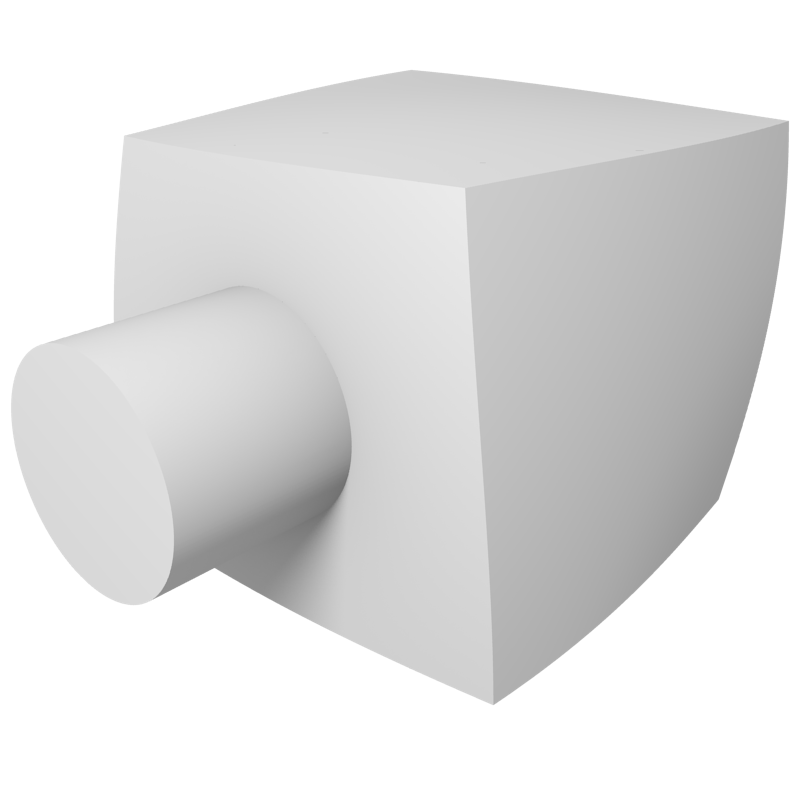
\includegraphics[width=\imagewidth]{piecewise_smooth_surface/surface}};
	%%% HIDDEN EDGES
	\node[img] at (0,0) {
\includegraphics[width=\imagewidth]{piecewise_smooth_surface/edges_hidden}};
	%%% HIDDEN CORNERS
	\DTLforeach*{dbcorners}{\locx=x, \locy=y, \loca=a}{%
		\ifnum \loca = 0
			\fill[black] (\locx,\locy) circle (1.0pt);
		\fi
	}%
	%%% SURFACE (semi-transparent to mask hidden edges & corners)
	{\transparent{0.75}
		\node[img] at (0,0) {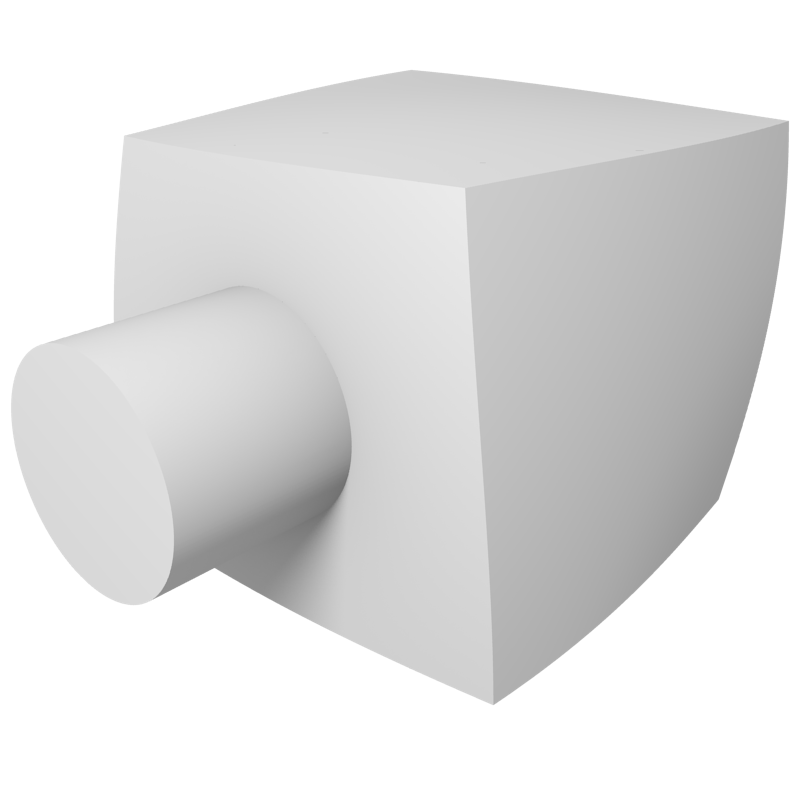
\includegraphics[width=\imagewidth]{piecewise_smooth_surface/surface}};
	}%
	%%% VISIBLE EDGES
	\node[img] at (0,0) {
\includegraphics[width=\imagewidth]{piecewise_smooth_surface/edges_visible}};
	%%% VISIBLE CORNERS
	\DTLforeach*{dbcorners}{\locx=x, \locy=y, \loca=a}{%
		\ifnum \loca = 1
			\fill[black] (\locx,\locy) circle (1.2pt);
		\fi
	}%
	%
	%%% ANOTATIONS
	\DTLassign{dbcorners}{6}{\locxa=x,\locya=y,\loca=a}% 	
	\DTLassign{dbcorners}{4}{\locxb=x,\locyb=y,\loca=a}% 
	\DTLassign{dbcorners}{1}{\locxc=x,\locyc=y,\loca=a}% 
	%\node[anchor=west] (anotSingPts) at (\locxb,{0.5*(\locya + \locyb)}) {points singuliers};
	\node[anchor=east] (anotSingPts) at (1.2,0.2) {coins};
	\draw[anot] (anotSingPts) to [bend left=10] (\locxa, \locya);
	\draw[anot] (anotSingPts) to [bend right=20] (\locxb, \locyb);
	\draw[anot] (anotSingPts) to [bend right=10] (\locxc, \locyc);
	%
	\DTLassign{dbedgemidp}{19}{\locxa=x,\locya=y,\loca=a}% 	
	\DTLassign{dbedgemidp}{7}{\locxb=x,\locyb=y,\loca=a}% 
	\DTLassign{dbedgemidp}{14}{\locxc=x,\locyc=y,\loca=a}% 
	\node[anchor=west] (anotSingCurv) at (-0.2,0.9) {crêtes};
	\draw[anot] (anotSingCurv) to [bend right=10] (\locxa, \locya);
	\draw[anot] (anotSingCurv) to [bend right=40] (\locxb, \locyb);
	\draw[anot] (anotSingCurv.east) to [bend left=10] (\locxc, \locyc);
\end{tikzpicture}
\DTLgdeletedb{dbcorners}%
\DTLgdeletedb{dbedgemidp}%

	\caption{Surface régulière \piecewise\ dont les courbes et points singuliers sont mis en évidence.}
	\label{fig:piecewise_smooth_surface_decomposition}
\end{figure}

%La frontière $\boundary{\Omega}$ du solide $\Omega$ est une surface de continuité $\contgeom{1}$ (\ie possède une direction normale continue) \piecewise. 
%Les singularités géométriques de $\boundary{\Omega}$ peuvent être de dimension 1 (courbes) ou 0 (points).
%Les courbes singulières de $\boundary{\Omega}$ sont elle-mêmes des variétés différentielles de continuité $\contgeom{1}$ (\ie possède une direction tangente continue) excepté aux points singuliers.

\subsection{Représentation par les frontières (\brep)}
%Origine, utilisation, concept, définitions formelles des entités, lien avec la décomposition d'une surface $\contgeom{1}$ \piecewise, (géométrie différentielle des courbes et surfaces paramétriques), structures de données (DCEL)
La \textit{représentation par les frontières} (ou \brep\ pour \anglais{Boundary Representation}) est un formalisme très répandu dans le domaine de la Conception Assistée par Ordinateur (CAO) \textit{(développer \ldots)}.
Elle consiste à décrire un solide $\Omega$ à l'aide d'une décomposition cellulaire de la surface $\Sigma$ qui matérialise sa frontière. 
Cette décomposition --- illustrée sur la \autoref{fig:BRep} --- est constituée de \textit{faces}, d'\textit{arêtes} et de \textit{sommets} dont on donne une définition dans les paragraphes suivants. 

\begin{figure}
	\centering
	\setlength{\imagewidth}{80mm}%
\setlength{\imageheight}{\imagewidth}%
\DTLsetseparator{,}%
\DTLloaddb[noheader,keys={x,y,a}]{dbverts}{figures/data/BRep/verts_xya.dat}%
\begin{tikzpicture}[%
	x=\imagewidth, y=\imageheight,
	img/.style={anchor=south west, inner sep=0}]
	%%%%%%%%%%%%%%%% SHELL %%%%%%%%%%%%%%%%
	%%% FACES
	\node[img] at (0,0) {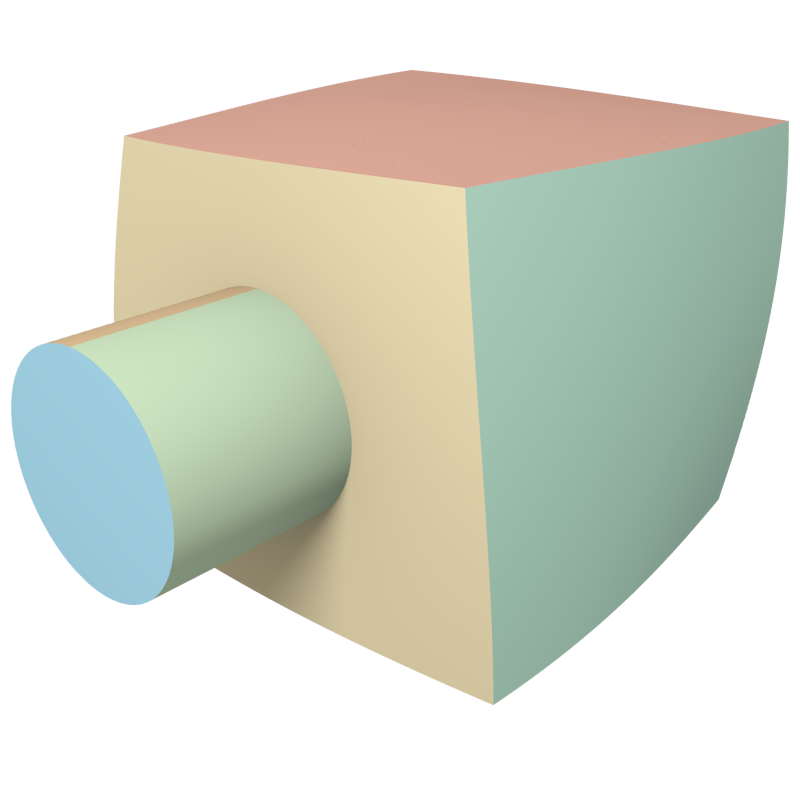
\includegraphics[width=\imagewidth]{BRep/shell}};
	%%% HIDDEN EDGES
	\node[img] at (0,0) {
\includegraphics[width=\imagewidth]{BRep/edges_hidden}};
	%%% HIDDEN VERTICES
	\DTLforeach*{dbverts}{\locx=x, \locy=y, \loca=a}{%
		\ifnum \loca = 0
			\fill[black] (\locx,\locy) circle (1.0pt);
		\fi
	}%
	%%% FACES (semi-transparent to mask hidden edges & verts)
	{\transparent{0.75}
		\node[img] at (0,0) {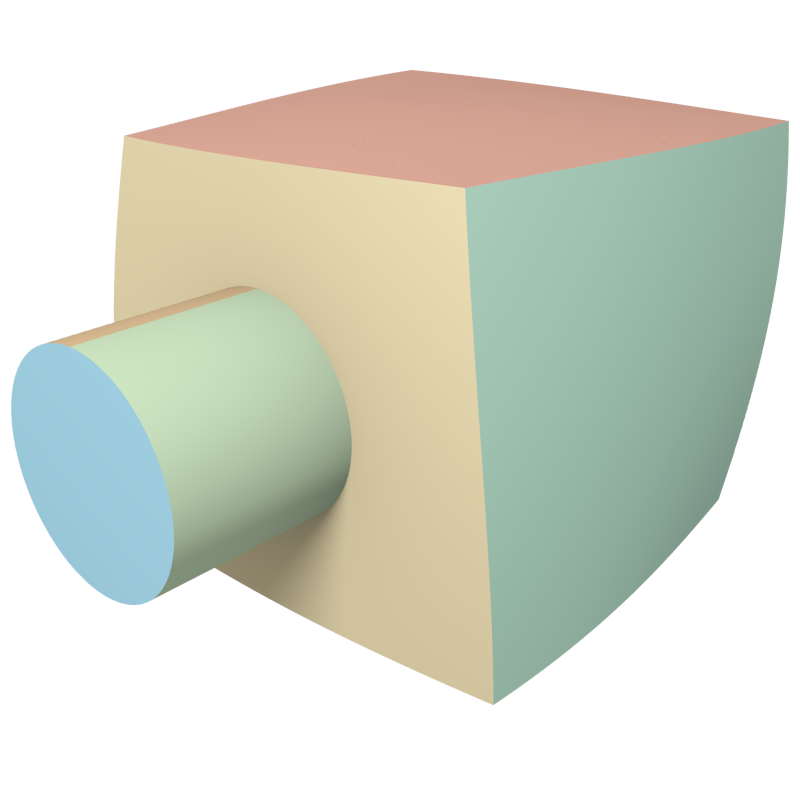
\includegraphics[width=\imagewidth]{BRep/shell}};
	}%
	%%% VISIBLE EDGES
	\node[img] at (0,0) {
\includegraphics[width=\imagewidth]{BRep/edges_visible}};
	%%% VISIBLE VERTICES
	\DTLforeach*{dbverts}{\locx=x, \locy=y, \loca=a}{%
		\ifnum \loca = 1
			\fill[black] (\locx,\locy) circle (1.0pt);
		\fi
	}%
\end{tikzpicture}
\DTLgdeletedb{dbverts}%
%%%%%%%%%%%%%%%%%%%%%%%%%%%%%%%%%%%%%%
%
%%%%%%%%%%%%%%%% FACES %%%%%%%%%%%%%%%%
\def\imfacew{44mm}
\def\ngriduv{6}
\def\vertsep{0.05}
\def\edglabsepuv{0.17}
\def\wirlabsepuv{0.18}
\def\edglabsepxyz{0.06}
\def\iniwclr{0.3}
\def\decwclr{0.3}%{0.2}
\def\uvscale{0.34}
\def\uvyshift{-0.7}
\pgfmathsetmacro\sepyshift{0.5 * (\uvyshift+\uvscale)}%
%
\begin{tikzpicture}[%
	x = \imfacew, y = \imfacew,
	gridtick/.style={red, fill=white, font=\tiny, inner sep=0.5pt},
	img/.style={anchor=south west, inner sep=0},
	label/.style={inner sep=1pt, font=\scriptsize},
	uvgrid/.style={black!10!white},
	curv/.style={line width=0.8pt, line cap=round},
	spacelabel/.style={anchor=north, rotate=90, inner sep=0, font=\bfseries},
	]
	\foreach \jfa/\ifa in {-1/007, 0/008, 1/002}{%
		\figbrepface{\ifa}{{1.05*\jfa - 0.5}}{{-\sepyshift}}%\hfill
	}%
	\draw[very thick, gray, dashed] 
	({-0.5*\textwidth},0) -- ++ 
	(\textwidth,0);
	\node[spacelabel] (xyzspace) at 
	({-0.5*\textwidth},{-\sepyshift+0.5}) {Espace euclidien\vphantom{Espace paramétrique}};
	\node[spacelabel] (uvspace) at 
	({-0.5*\textwidth},{\sepyshift-\uvscale}) {Espace paramétrique\vphantom{Espace euclidien}};
\end{tikzpicture}

	\caption{Modèle \brep\ d'une surface régulière par morceaux.}
	\label{fig:BRep}
\end{figure}

\subsubsection{Faces}
\label{section:def_brep_faces}
Une face du modèle \brep\ est une variété de dimension 2 connexe délimitée par des arêtes et des sommets. 
Géométriquement, une face $\brepface$ est décrite par un carreau paramétrique restreint.
La topologie des courbes de restriction du domaine paramétrique est décrite à l'aide de \textit{contours} (un par composante connexe du bord de $\brepface$). 
Une face possède ainsi un contour extérieur $\brepwire^{\mathrm{ext}}$ et, éventuellement un ou plusieurs contours intérieurs $\brepwire^{\mathrm{int},i}$ si celle-ci comporte des \guillemets{trous}.
Les faces, qui sont quasi-disjointes deux-à-deux (\ie ne s'intersectent qu'en des arêtes ou des sommets du modèle \brep), sont regroupées en \textit{coquilles}, qui représentent chacune une composante connexe de $\Sigma$. 


\subsubsection{Arêtes}
\label{section:def_brep_edges}
Une arête du modèle \brep\ est une variété de dimension 1 connexe délimitée par des sommets.
Puisque $\Sigma$ est une variété sans bord, chaque arête du modèle \brep\ est incidente à exactement deux faces $\brepface_1$ et $\brepface_2$. 
Géométriquement, l'arête $\brepedge$ est représentée par une branche de la courbe d'intersection entre les carreaux $\Sigma_1$ et $\Sigma_2$ qui décrivent respectivement $\brepface_1$ et $\brepface_2$. 
Cette courbe peut également être représentée par sa trace dans l'espace paramétrique de chaque carreau. 
On peut donc la représenter à l'aide des trois courbes paramétriques $\bg$, $\bp_1$ et $\bp_2$ telles que
\begin{equation}
	\bg = \bs_1 \circ \bp_1 = \bs_2 \circ \bp_2.
\end{equation}

\begin{figure}
	\centering
	\setlength{\imagewidth}{67.5mm}
\setlength{\imageheight}{\imagewidth * \real{0.75}}
%
\def\uvscale{0.28}
\def\fracaxeoffset{0.0}
\def\distanceaxe{0.1}
\def\psisep{-0.42}
%
\DTLsetseparator{,}%
\DTLloaddb[noheader,keys={x,y}]{dbpoint}{figures/data/simple_intersection/point.dat}%
\DTLassign{dbpoint}{1}{\xloc=x, \yloc=y}% 
%
\begin{tikzpicture}[
	x=\imagewidth, y=\imageheight, 
	axe/.style={-stealth, line width=0.5pt},
	uvdomain/.style={thin}, 
	image/.style={anchor=south west, inner sep=0},
	curve/.style={thick, line cap=round},
	label/.style={font=\normalsize},
	axelabel/.style={font=\small},
	axeuvlabel/.style={axelabel, inner sep=0},
	point/.style={fill=black, circle, scale=0.3},
	map/.style={-{Classical TikZ Rightarrow[length=4pt,width=4pt]}}]
	%
	\node[image] (img) at (0,0) {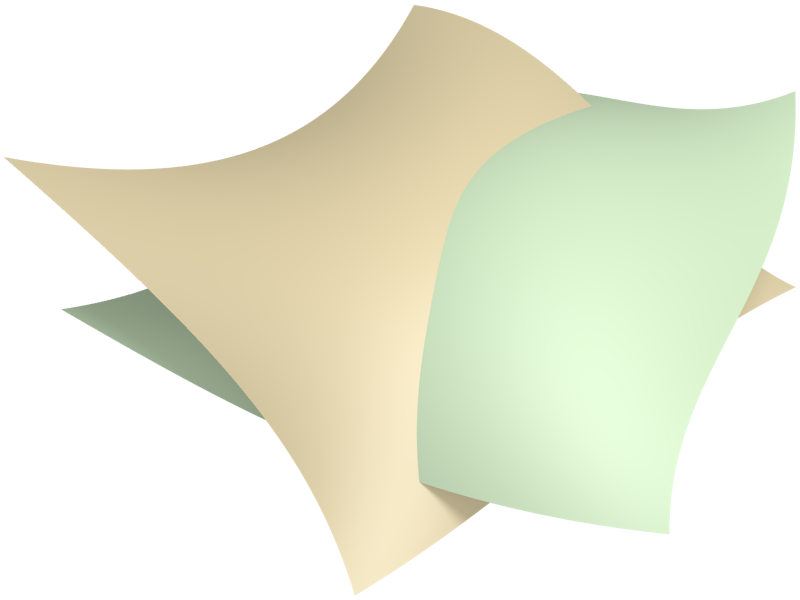
\includegraphics[width=\imagewidth]{figures/images/simple_intersection/surfaces}};
	\node[image] (img) at (0,0) {
\includegraphics[width=\imagewidth]{figures/images/simple_intersection/borders_hidden}};
	{\transparent{0.75}%
		\node[image] (img) at (0,0) {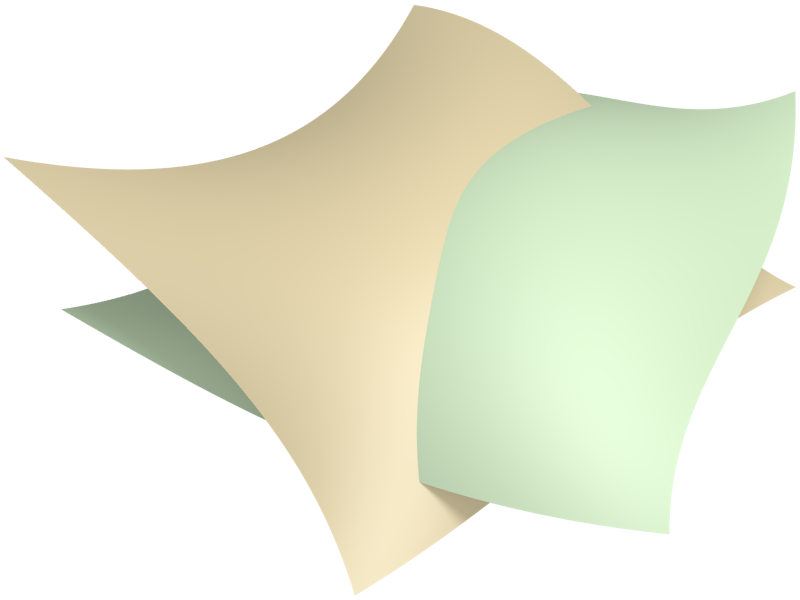
\includegraphics[width=\imagewidth]{figures/images/simple_intersection/surfaces}};
	}%
	\node[image] (img) at (0,0) {
\includegraphics[width=\imagewidth]{figures/images/simple_intersection/borders_visible}};
	\draw[curve] plot file {figures/data/simple_intersection/curve_xy.dat};
	\node[point] (xyz) at (\xloc, \yloc) {};
	\node[label, anchor=east] at (\xloc, \yloc) {$\bg(w)$};
	%
	\node[label] at (0.56, 0.91) {$\Sigma_1$};
	\node[label] at (0.93, 0.75) {$\Sigma_2$};
	%
%	\foreach \igrid in  {0,0.1,...,1.01}{
%		\draw[red, thin] (0,\igrid) -- (1,\igrid)
%		                 (\igrid,0) -- (\igrid,1);
%	}
	% 
	% trièdre
	\def\scaletriedre{0.8}
	\coordinate (o) at (0.13209545612335205 , 0.14773482084274292);
	\coordinate (x) at (0.23464959859848022 , 0.02938912808895111);
	\coordinate (y) at (0.26169726252555847 , 0.2535654902458191);
	\coordinate (z) at (0.1061694324016571 , 0.31903284788131714);
	\draw[axe] (o) -- ($(o)!\scaletriedre!(x)$) node[axelabel, anchor=west] {$x$};
	\draw[axe] (o) -- ($(o)!\scaletriedre!(y)$) node[axelabel, anchor=west] {$y$};
	\draw[axe] (o) -- ($(o)!\scaletriedre!(z)$) node[axelabel, anchor=south] {$z$};
	%
	\begin{scope}[scale=\uvscale, x=\imageheight, y=\imageheight, shift={(img.west)}]
		\begin{scope}[shift={(-1.5,0.7)}]
			\DTLloaddb[noheader,keys={r,g,b}]{dbsurfacecolor}{figures/data/BRep/faces/facecolor_002.dat}%
			\DTLassign{dbsurfacecolor}{1}{\rfai=r,\gfai=g,\bfai=b}% 
			\definecolor{surfacecolor}{RGB}{\rfai,\gfai,\bfai}
			\draw[uvdomain, fill=surfacecolor] (-1,-1) -- (1,-1) -- (1,1) -- (-1,1) -- cycle;
			\DTLgdeletedb{dbsurfacecolor}
			%
			\draw[curve] plot file {/d/bandrieu/GitHub/FFTsurf/test/demo_intersection/simple/curve_uv1.dat};
			%
			\DTLassign{dbpoint}{2}{\uloc=x, \vloc=y}% 
			\DTLassign{dbpoint}{3}{\duloc=x, \dvloc=y}% 
			\node[point] (uv1) at (\uloc, \vloc) {};
			%\node[label] at ({\uloc + \psisep*\duloc}, {\vloc + \psisep*\dvloc}) {$\bp_1(w)$};
			\node[label, anchor=north east, inner sep=0] at (\uloc, \vloc) {$\bp_1(w)$};
			% Axes
			\coordinate (o) at ({-1-\distanceaxe},{-1-\distanceaxe});
			\draw[axe] (o) -- ++ ({\fracaxeoffset+\distanceaxe+0.5},0) node [axeuvlabel, anchor=north west] {$u_1$};
			\draw[axe] (o) -- ++ (0,{\fracaxeoffset+\distanceaxe+0.5}) node [axeuvlabel, anchor=south east] {$v_1$};
		\end{scope}
	\end{scope}
	%
	\begin{scope}[scale=\uvscale, x=\imageheight, y=\imageheight, shift={(img.east)}]
		\begin{scope}[shift={(1.6,-0.9)}]
			\DTLloaddb[noheader,keys={r,g,b}]{dbsurfacecolor}{figures/data/BRep/faces/facecolor_008.dat}%
			\DTLassign{dbsurfacecolor}{1}{\rfai=r,\gfai=g,\bfai=b}% 
			\definecolor{surfacecolor}{RGB}{\rfai,\gfai,\bfai}
			\draw[uvdomain, fill=surfacecolor] (-1,-1) -- (1,-1) -- (1,1) -- (-1,1) -- cycle;
			\DTLgdeletedb{dbsurfacecolor}
			%
			\draw[curve] plot file {/d/bandrieu/GitHub/FFTsurf/test/demo_intersection/simple/curve_uv2.dat};
			%
			\DTLassign{dbpoint}{4}{\uloc=x, \vloc=y}% 
			\DTLassign{dbpoint}{5}{\duloc=x, \dvloc=y}% 
			\node[point] (uv2) at (\uloc, \vloc) {};
			%\node[label] at ({\uloc + \psisep*\duloc}, {\vloc + \psisep*\dvloc}) {$\bp_2(w)$};
			\node[label, anchor=north east, inner sep=0] at (\uloc, \vloc) {$\bp_2(w)$};
			% Axes
			\coordinate (o) at ({-1-\distanceaxe},{-1-\distanceaxe});
			\draw[axe] (o) -- ++ ({\fracaxeoffset+\distanceaxe+0.5},0) node [axeuvlabel, anchor=north west] {$u_2$};
			\draw[axe] (o) -- ++ (0,{\fracaxeoffset+\distanceaxe+0.5}) node [axeuvlabel, anchor=south east] {$v_2$};
		\end{scope}
	\end{scope}
	%
	% mappings
	\draw [map, shorten <= 5mm, shorten >= 5mm] (uv1) to [bend left =40] node [label, anchor=south west] {$\bs_1$} (xyz);
	\draw [map, shorten <= 5mm, shorten >= 5mm] (uv2) to [bend right=40] node [label, anchor=south west] {$\bs_2$} (xyz);
	%
%	\draw[red, thin, dashed] (current bounding box.south west) rectangle (current bounding box.north east);
\end{tikzpicture}
\DTLgdeletedb{dbpoint}
	\caption{Description géométrique d'une arête \brep.}
\end{figure}

Les arêtes, qui sont quasi-disjointes deux-à-deux (\ie ne s'intersectent qu'en des sommets du modèle \brep), sont regroupées pour former les contours des faces. 
Puisque ces derniers sont orientés, chaque arête $\brepedge$ est formée de deux \textit{co-arêtes} jumelles $\brepedge^1$ et $\brepedge^2$, chacune associée à une face incidente à $\brepedge$. 
Chaque co-arête possède une orientation, conforme à celle du contour qui la contient.


\subsubsection{Sommets}
\label{section:def_brep_vertices}
Un sommet du modèle \brep\ matérialise l'intersection de deux arêtes et a pour support géométrique un point de $\reals^3$.

\subsubsection{Structure de données}
\begin{enumerate}
	\item séparation entre topologie (structure) / géométrie (forme)
	\item connectivité entre les entités capturée à l'aide d'une structure de graphe (homéomorphe à un polyèdre)
	\item structure de données adaptée $\to$ \anglais{Doubly Connected Edge List} (DCEL) (\anglais{Halfedges}) \textit{(donner réfs.)}
\end{enumerate}

La \autoref{fig:BRep_hierarchy} présente un diagramme de la hiérarchie des entités qui constituent le modèle \brep.
\begin{figure}
	\centering
	\colorlet{topo_color}{mycolor_5}
\colorlet{orient_color}{topo_color!60!mycolor_2}
\colorlet{group_color}{topo_color!40!mycolor_3}
\colorlet{geom_color}{mycolor_1}%{mycolor_3}
\def\bigsep{5mm}
\def\smallsep{2.5mm}
\pgfdeclarelayer{bg}    % declare background layer
\pgfsetlayers{bg,main}  % set the order of the layers (main is the standard layer)
\begin{tikzpicture}[
	x = 30mm,
	y = 9.75mm,
	arrow/.style={thick, -stealth', shorten <= 2pt, shorten >= 2pt},
	bounded/.style={arrow, dash pattern=on 4pt off 2pt},
	described/.style={arrow},
	composed/.style={arrow, dash pattern=on 1.5pt off 1.5pt},
	box/.style={rectangle, rounded corners=0.8ex},
	number/.style={font=\footnotesize},
	topo/.style={fill=topo_color!33!white},
	geom/.style={fill=geom_color!33!white},
	orient/.style={fill=orient_color!33!white},
	group/.style={fill=group_color!33!white},
	type/.style={font=\bfseries},%, anchor=east},
	label/.style={anchor=west, inner sep=2pt, font=\scriptsize},
	class/.style={dotted, thick, line cap=round},
	bigclass/.style={class, rounded corners=\bigsep, dash pattern=on 0.8pt off 3.2pt},
	smallclass/.style={class, rounded corners=\smallsep, dash pattern=on 0.3pt off 2.8pt},
	]
	% entités topologiques
	\node[box, topo] at (-1,1) (volume) {Solide};
	\node[box, topo] at (0,1) (face) {Face};
	\node[box, topo] at (1,1) (edge) {Arête};
	\node[box, topo] at (2,1) (vertex) {Sommet};
	% entités de groupement
	\node[box, group] at (-1,3) (shell) {Coquille};
	\node[box, group] at (0,3) (wire) {Contour};
	% entités d'orientation
	\node[box, orient] at (1,3) (halfedge) {Co-arête};
	% entités géométriques
	\node[box, geom] at (0,-1) (surface) {Surface};
	\node[box, geom] at (1,-1) (curve) {Courbe};
	\node[box, geom] at (2,-1) (point) {Point};
	%
	% relations "décrit par"
	\draw[described] (face) -- (surface);
	\draw[described] (edge) -- (curve);
	\draw[described] (vertex) -- (point);
	% relations "délimité par"
	\draw[bounded] (volume) -- 
		node[number,left]{$1+n_{\mathrm{s}}^{\mathrm{int}}$} 
		(shell);
	\draw[bounded] (face) -- 
		node[number,right]{$1+n_{\mathrm{w}}^{\mathrm{int}}$} 
		(wire);
	\draw[bounded] (edge) -- node[number,above]{$2$} (vertex);
	% relations "composé de"
	\draw[composed] (shell) -- node[number,above right]{$n$} (face);
	\draw[composed] (wire) -- node[number,above]{$n$} (halfedge);
	\draw[composed] (edge) -- node[number,right]{$2$} (halfedge);
	%
	% noms de classes
	\gettikzxy{(current bounding box.east)}{\xbbE}{\ybbE}%
	\node[type, geom_color!90!gray] (geomet) at (-1,-1) {Géométrie};
	\node[type, anchor=east, orient_color!90!gray] (orientation) at ({\xbbE-0.5*\smallsep},3) {Orientation};
	\gettikzxy{(halfedge.east)}{\xhE}{\yhE}%
	\gettikzxy{(orientation.west)}{\xoW}{\yoW}%
	\gettikzxy{(shell.west)}{\xsW}{\ysW}%
	\node[type, anchor=east, group_color!90!gray] (grouping) at ({\xsW-\xoW+\xhE},3) {Groupement};
	\gettikzxy{(grouping.west)}{\xgrW}{\ygrW}%
	\gettikzxy{(grouping.south)}{\xgrS}{\ygrS}%
	\gettikzxy{(volume.south)}{\xvS}{\yvS}%
	\node[type, anchor=west, topo_color!90!gray] (topology) at (\xgrW,{0.5*(\ygrS-\smallsep + \yvS-\bigsep)}) {Topologie};
	%
	% classes
	\gettikzxy{(vertex.south east)}{\xtSE}{\ytSE}%
	\gettikzxy{(shell.north)}{\xtN}{\ytN}%
	\gettikzxy{(grouping.west)}{\xtW}{\ytW}%
	\gettikzxy{(geomet.west)}{\xgeW}{\ygeW}%
	\gettikzxy{(topology.north)}{\xtM}{\tmp}%
	\gettikzxy{(grouping.south)}{\tmp}{\ytM}%
	\gettikzxy{(halfedge.south west)}{\xoSW}{\yoSW}%
	\gettikzxy{(halfedge.north)}{\xoN}{\yoN}%
	\gettikzxy{(orientation.north east)}{\xoNE}{\yoNE}%
	\gettikzxy{(grouping.south west)}{\xgrSW}{\ygrSW}%
	\gettikzxy{(wire.south)}{\xgrS}{\ygrS}%
	\gettikzxy{(wire.north east)}{\xgrNE}{\ygrNE}%
	\gettikzxy{(surface.south)}{\xgeS}{\ygeS}%
	\gettikzxy{(surface.north)}{\xgeN}{\ygeN}%
	\begin{pgfonlayer}{bg}    % select the background layer
		\draw[bigclass, topo_color, fill=topo_color!8!white] 
		({\xtSE+\bigsep},{\ytSE-\bigsep}) --
		({\xtSE+\bigsep},{\ytN+\bigsep}) --
		({\xtW-\bigsep},{\ytN+\bigsep}) --
		({\xtW-\bigsep},{\ytSE-\bigsep}) -- cycle;
		%
		\draw[smallclass, orient_color, fill=orient_color!8!white] 
		({\xoSW-\smallsep},{\yoSW-\smallsep}) -- 
		({\xoNE+\smallsep},{\yoSW-\smallsep}) -- 
		({\xoNE+\smallsep},{\yoN+\smallsep}) -- 
		({\xoSW -\smallsep},{\yoN+\smallsep}) -- cycle;
		%
		\draw[smallclass, group_color, fill=group_color!8!white] 
		({\xgrSW-\smallsep},{\ygrS-\smallsep}) -- 
		({\xgrNE+\smallsep},{\ygrS-\smallsep}) -- 
		({\xgrNE+\smallsep},{\ygrNE+\smallsep}) -- 
		({\xgrSW -\smallsep},{\ygrNE+\smallsep}) -- cycle;
		%
		\draw[bigclass, geom_color, fill=geom_color!8!white]
		({\xgeW-\bigsep},{\ygeS-\bigsep}) -- 
		({\xtSE+\bigsep},{\ygeS-\bigsep}) -- 
		({\xtSE+\bigsep},{\ygeN+\bigsep}) -- 
		({\xgeW-\bigsep},{\ygeN+\bigsep}) -- cycle;
	\end{pgfonlayer}
	% légende des relations
	\coordinate (lgd) at ({\xtW-\bigsep+2pt},{0.5*(\ygeS+\ygeN)});
	\foreach \i in {0,1,2}{
		\coordinate (L\i) at ([yshift={-(\i-1)*2.8ex}]lgd);
		\coordinate (R\i) at ([xshift=7.5mm]L\i);
	}
	\draw[described] (L0) -- (R0) node[label] (lbl0) {décrit par};
	\draw[bounded]   (L1) -- (R1) node[label] (lbl1) {délimité par};
	\draw[composed]  (L2) -- (R2) node[label] (lbl2) {composé de};
	\node[draw=black!25,
	inner sep=2pt,
	rounded corners=\smallsep,
	fit={(L0) (lbl0) (lbl1) (lbl2)}] {};
\end{tikzpicture}
	\caption{Hiérarchie des éléments constituant un modèle \brep.}
	\label{fig:BRep_hierarchy}
\end{figure}


\subsubsection{Représentation de surfaces régulières par morceaux}
Le formalisme de la représentation par les frontières est particulièrement adapté pour décrire des surfaces régulières par morceaux. 
En effet, 
\begin{itemize}
	\item l'ensemble des points singuliers de $\Sigma$ est un sous-ensemble des sommets de son modèle \brep\ ;
	\item l'ensemble des courbes singulières de $\Sigma$ est un sous-ensemble des arêtes de son modèle \brep\ ;
	\item les nappes régulières de $\Sigma$ sont formées par la réunion des faces de son modèle \brep.
%	\item chaque arête \brep\ vive est contenue dans une courbe singulière
\end{itemize}











\section{Formulation lagrangienne du problème de propagation d'interface}
On considère une interface $\Sigma$ entre deux milieux distincts (\eg un solide et un fluide).
Dans cette thèse, on se concentre sur des problèmes en trois dimensions. 
$\Sigma$ représente donc une surface (\ie une variété de dimension 2) que l’on supposera orientable et fermée (\ie sans bord).
De cette manière, l'interface sépare un domaine \textit{intérieur} $\Omega$ --- que l'on supposera ouvert --- et un domaine \textit{extérieur} $\complement{\Omega} = \reals^3 \setminus \Omega$ (voir \autoref{fig:schema_interface_2d}). 
$\Sigma$ est alors la frontière commune de ces domaines
\begin{equation}
	\Sigma = \boundary{\Omega} = \boundary{(\complement{\Omega})}.
\end{equation}
\par
%[EDP avec vecteur vitesse ou vitesse normale, problème de définition au niveau des courbes singulières et points irréguliers]
%\par\bigskip
Le problème que l'on cherche à résoudre consiste à déterminer l’évolution au cours du temps de l'interface $\Sigma$ étant données sa position actuelle ainsi que sa vitesse de propagation.
Dans la formulation lagrangienne traditionnelle, ce problème est exprimé sous la forme d'une équation aux dérivées partielles (EDP) pour le vecteur position $\bx$ d'un point de l'interface.
L'équation décrivant la propagation suivant un champ de vecteur vitesse $\vrm{u} : \Sigma \times \reals \to \reals^3$ est
\begin{equation}
	\frac{\partial \bx}{\partial t} = \vrm{u}(\bx,t).
	\label{eq:lagrange_vecteur_vitesse}
\end{equation}
On peut également considérer que chaque point de $\Sigma$ se déplace le long de la direction normale à l'interface suivant un champ de vitesse normale $\nu : \Sigma \times \reals \to \reals$. 
L'équation décrivant la propagation est alors
\begin{equation}
	\frac{\partial \bx}{\partial t} = \nu(\bx,t) \unv(\bx,t),
	\label{eq:lagrange_vitesse_normale}
\end{equation}
où $\unv(\bx,t)$ désigne la direction normale à $\Sigma$ en $\bx$ à l'instant $t$, pointant vers l'extérieur de $\Omega$.
\par\bigskip
En principe, les formulations \eqref{eq:lagrange_vecteur_vitesse} et \eqref{eq:lagrange_vitesse_normale} sont équivalentes puisque la composante tangentielle du vecteur vitesse n'affecte pas la forme de l'interface. 
\par\bigskip
La formulation lagrangienne ne permet d'obtenir une solution au problème de propagation d'interface que dans le cas où cette dernière est \textit{globalement} régulière et le reste tout au long de sa propagation. 
En effet, puisque la direction normale $\unv$ n'est pas définie au niveau des courbes et points singuliers de $\Sigma$, le déplacement de ces points est ambigu. 
On peut notamment distinguer deux cas \cite{jiao2007}.
\par
Premièrement, si l'interface subit un mouvement d'advection (comme le transport d'un fluide ou encore la déformation d'un solide sous l'effet de contraintes mécaniques) alors ses singularités géométriques sont préservées au cours de la propagation.
\par
En revanche, si l'interface se propage à la manière d'un front d'onde (comme la progression d'une flamme, d'un dépôt de matière ou encore l'ablation d'un solide) alors les singularités sont soit préservées soit régularisées, suivant la convexité locale de l'interface.
C'est essentiellement sur ce deuxième type de propagation que l'on se concentre dans cette thèse.
\par\bigskip
Puisque l'on s'intéresse ici à la propagation d'interfaces régulières seulement \piecewise, il est nécessaire d'obtenir une meilleure formulation du problème qui s'affranchisse des ambiguïtés ainsi mises en évidence. 
Plutôt que de poser le problème sous la forme d'une équation différentielle, cette nouvelle formulation se présente comme une construction géométrique.

\section{Principe de Huygens avec condition d'entropie}
\label{section:principe_huygens}
\def\p{\vit{p}}
\def\q{\vit{q}}
%
%[Histoire, formulation, notion d'enveloppe de sphères/boules, construction géométrique au lieu de EDP, équations définissant l'EdS propre à 1/2 paramètre(s), différence d'ordre 2 avec transport suivant la normale, définitions implicites (\cf notes Huygens)]
%\par\bigskip
Alors qu'il développait un modèle ondulatoire de la propagation de la lumière, Christiaan Huygens proposa le principe suivant : chaque point de l'espace atteint par une onde lumineuse se comporte comme la source d'une ondelette secondaire émise dans toutes les directions. 
Si le milieu de propagation est homogène et isotrope alors les ondelettes sont sphériques. 
Le front d'onde, qui se propage ainsi de proche en proche, est formé par l'\textit{enveloppe} de ces ondelettes, \ie la surface qui est tangente à chacune d'elles et dont chaque point est un point de tangence avec une ondelette.
\par
Le principe de Huygens permet de décrire de nombreux phénomènes analogues à la propagation d'une onde dans un milieu tels que la progression d'une flamme. 
\textit{(développer \ldots)}

\par\bigskip
\begin{enumerate}
	\item distinguer propagation d'une onde et d'une interface entre deux milieux matériels (l'une peut s'auto-intersecter, l'autre non) $\to$ condition d'entropie
	%\item formaliser la notion d'enveloppe des sphères $\EdS{\Sigma}{\rho}$ (surface tangente à toutes les sphères et en tout point tangente à une sphère) $\to$ système d'équations avec $\implicitsphere_{\rho} : (\bx,\p) \mapsto \normtwo{\bx - \p}^2 - \rho^2(\p)$
	%\item formaliser la notion d'enveloppe des boules $\EdB{\Sigma}{\rho} := \boundary{\left\{\Omega \cup \sphere[\Sigma][\rho]\right\}}$
	\item formaliser la notion d'enveloppe des sphères (EdS) $\EdS{H \subseteq \Sigma}{\rho}$ (surface tangente à toutes les sphères et en tout point tangente à une sphère)
	%\item formaliser la notion d'enveloppe des boules $\EdB{\Sigma}{\rho} := \boundary{\left\{\Omega \cup \sphere[\Sigma][\rho]\right\}}$
	\item formaliser la notion d'enveloppe des boules (EdB) $\EdB{H \subseteq \Sigma}{\rho} := \boundary{ \left( \ball{H}{\rho} \right) }$
	\item si $H \subseteq \Sigma$ est une variété sans bord alors $\EdB{H}{\rho}  = \EdBplus{H}{\rho} \cup \EdBmoins{H}{\rho}$ où $\EdBplus{H}{\rho} \subset \complement{\Omega}$ et $\EdBmoins{H}{\rho} \subset \Omega$ (car $\rho > 0$) \textit{(illustrer)}\\
	$\Rightarrow$ en particulier, $\EdB{\Sigma}{\rho}  = \EdBplus{\Sigma}{\rho} \cup \EdBmoins{\Sigma}{\rho}$
	
	
	\item donner définition implicite de l'EdB :\\
	on pose 
	\[
		\implicitsphere(\bx, \p) := \normtwo{\bx - \p}^2 - \rho(\p)^2,
	\]
	et, pour $H \subseteq \Sigma$, 
	\[
		\implicitEdB{H}(\bx) := \min_{\p \in H} \implicitsphere(\bx, \p).
	\]
	Alors,
	\[ 
		\EdB{H}{\rho} 
		= \implicitEdB{H}^{-1}(0)
		= 
		\left\{
			\bx \in \reals^3 \mid \forall \p \in H, \implicitsphere(\bx, \p) \geq 0
			\text{ et } \exists \q \in H \mid \implicitsphere(\bx, \p) = 0
		\right\}.
	\]
	\item après une propagation à vitesse normale $\nu$ constante pendant un intervalle de temps $\tau$ tel que $\nu \tau = \rho$, la nouvelle interface est $\EdBplus{\Sigma}{\rho}$
	\item à condition que $\rho$ soit suffisamment régulière (continuité à déterminer), $\EdB{\Sigma}{\rho} \subseteq \EdS{\Sigma}{\rho}$
	\item si $\EdS{\Sigma}{\rho}$ ne présente pas d'auto-intersections alors $\EdB{\Sigma}{\rho} = \EdS{\Sigma}{\rho}$
\end{enumerate}


%%%%%%%%%%%%%%%%%%%%%%%%%%%%%%%%%%%%%%%%%%%
%%%%%%%%%%%%%%%%%%%%%%%%%%%%%%%%%%%%%%%%%%%
\def\pathSigma{(-0.06745414982903328, -0.48958657133975747) .. controls (0.37550512900217586,-0.48958657133975747) and (0.39881877525645004,-0.46627292508548335) .. (0.39881877525645004,-0.44295927883120917) --
(0.39881877525645004, -0.44295927883120917) .. controls (0.39881877525645004,-0.4243202171683753) and (0.49816391583257014,-0.3758776133327055) .. (0.5380030090663426,-0.2857176282303145) --
(0.5380030090668455, -0.2857176282306956) .. controls (0.8699520768979537,-0.1856533318838257) and (0.6967963209781135,0.1474709569716339) .. (0.95834628535903,0.2564501087970158) --
(0.95834628535903, 0.2564501087970158) .. controls (0.9863226608641589,0.2681069319241529) and (0.9993783027665525,0.27603357165060616) .. (0.9999999999999999,0.2791109729561704) --
(0.9999999999999999, 0.2791109729561704) .. controls (0.8340068386695678,0.27976375505129003) and (0.8029219769972022,0.27976375505129003) .. (0.7718371153248368,0.2564501087970158) --
(0.7718371153248368, 0.2564501087970158) .. controls (0.6581503320934389,0.1711850213734677) and (0.7263704078262674,-0.011530169066630227) .. (0.5250514731877045,-0.04221221894306825) --
(0.525051473207803, -0.04221221895613872) .. controls (0.49540859687413463,0.05361148339987804) and (0.4471136860652924,0.15503079609844692) .. (0.39881877525645004,0.2564501087970158) --
(0.39881877525645004, 0.2564501087970158) .. controls (0.3891047559838358,0.2768495492695058) and (0.37647653092943734,0.2870492695057507) .. (0.3687053155113459,0.2870492695057507) --
(0.3687053155113459, 0.2870492695057507) .. controls (0.3392257446993408,0.28704926950434584) and (0.3097461738873358,0.28704926950294096) .. (0.28026660307533063,0.2870492695015359) --
(0.28026660307533063, 0.2870492695015359) .. controls (0.19519421128589576,0.306844207600626) and (0.03921493352678685,0.31633017380579564) .. (-0.005284426484302166,0.34970469381411257) --
(-0.005284426484302166, 0.34970469381411257) .. controls (-0.06745414982903328,0.39633198632266087) and (0.18122474354989118,0.48958657133975747) .. (-0.06745414982903328,0.48958657133975747) --
(-0.06745414982903328, 0.48958657133975747) .. controls (-0.3161330432079577,0.48958657133975747) and (-0.06745414982903328,0.39633198632266087) .. (-0.1296238731737644,0.34970469381411257) --
(-0.1296238731737644, 0.34970469381411257) .. controls (-0.1741232331848534,0.31633017380579564) and (-0.33010251094396226,0.306844207600626) .. (-0.4151749027333972,0.2870492695015359) --
(-0.4151749027333972, 0.2870492695015359) .. controls (-0.44465447354540233,0.28704926950294096) and (-0.47413404435740736,0.28704926950434584) .. (-0.5036136151694125,0.2870492695057507) --
(-0.5036136151694125, 0.2870492695057507) .. controls (-0.5113848305875038,0.2870492695057507) and (-0.5240130556419024,0.2768495492695058) .. (-0.5337270749145167,0.2564501087970158) --
(-0.5337270749145167, 0.2564501087970158) .. controls (-0.5411317420051683,0.240900307906647) and (-0.54853640909582,0.22535050701627826) .. (-0.5558738499625876,0.20982087399307478) --
(-0.5558738257524533, 0.20982087345806888) .. controls (-0.8519579419174843,0.20974199165489985) and (-0.9999999999999999,0.20646039134599314) .. (-0.9999999999999999,0.06994093876282252) --
(-0.9999999999999999, 0.06994093876282252) .. controls (-0.9999999999999999,-0.06828571804650066) and (-0.8937625382099367,-0.19512978966403147) .. (-0.6662904210477201,-0.29934338090320184) --
(-0.66629042098975, -0.29934338083854817) .. controls (-0.6230838887209378,-0.38079774574522973) and (-0.5337270749145167,-0.4252820343591826) .. (-0.5337270749145167,-0.44295927883120917) --
(-0.5337270749145167, -0.44295927883120917) .. controls (-0.5337270749145167,-0.46627292508548335) and (-0.5104134286602424,-0.48958657133975747) .. (-0.06745414982903328,-0.48958657133975747) --
cycle (-0.588330877270558, 0.13987844696398508) .. controls (-0.6441171041265075,0.01665754175696133) and (-0.6891513832763444,-0.1033377791382286) .. (-0.6891513832763444,-0.20982281628846747) --
(-0.6891513832763444, -0.20982281628846747) .. controls (-0.8445756916381721,-0.139881877525645) and (-0.9067454149829033,0.0) .. (-0.9067454149829033,0.06994093876282252) --
(-0.9067454149829033, 0.06994093876282252) .. controls (-0.9067454149829033,0.1373216629971834) and (-0.7913423441785001,0.13978815990406745) .. (-0.5883308770022139,0.13987844695664525) --
cycle}
\def\pathEdSplus{(-0.06957787148578239, -0.5304982349142947) -- (-0.05625729027974507, -0.5311801914104046) -- (-0.04317770697493112, -0.5318288771980217) -- (-0.03033684263301526, -0.5324420903836042) -- (-0.017732542228013553, -0.533017985749606) -- (-0.005362760790061074, -0.5335550618168393) -- (0.006774451871234943, -0.5340521449176762) -- (0.01868096729078475, -0.5345083708827423) -- (0.03035859479235303, -0.5349231648956592) -- (0.041809097786652705, -0.5352962200224056) -- (0.05303420952586474, -0.5356274748741706) -- (0.0640356479906066, -0.5359170908153119) -- (0.07481512965885956, -0.5361654290813992) -- (0.0853743819768484, -0.5363730281265332) -- (0.09571515441701366, -0.536540581474504) -- (0.10583922806642895, -0.536668916305214) -- (0.11574842373933504, -0.5367589729665272) -- (0.1254446086494932, -0.5368117855626668) -- (0.1349297017118258, -0.5368284637338222) -- (0.14420567756869687, -0.5368101757080178) -- (0.15327456945479542, -0.5367581326757705) -- (0.16213847102671144, -0.5366735745107514) -- (0.17079953728979547, -0.5365577568356582) -- (0.17925998475667373, -0.5364119394117611) -- (0.18752209096974598, -0.5362373758130404) -- (0.19558819351494908, -0.5360353043313403) -- (0.20346068864681127, -0.5358069400473202) -- (0.21114202963603057, -0.5355534679929629) -- (0.2186347249410782, -0.5352760373247234) -- (0.22594133629515858, -0.5349757564218103) -- (0.23306447678965872, -0.5346536888212687) -- (0.24000680902531724, -0.534310849900217) -- (0.2467710433929811, -0.5339482042154737) -- (0.25335993653717076, -0.5335666634116382) -- (0.2597762900478653, -0.5331670846101977) -- (0.2660229494190021, -0.5327502691941801) -- (0.2721028033061967, -0.5323169619050363) -- (0.27801878311108885, -0.5318678501706076) -- (0.28377386291549944, -0.5314035635850226) -- (0.2893710597851309, -0.5309246734629826) -- (0.2948134344597969, -0.5304316923919774) -- (0.300104092444992, -0.5299250737063589) -- (0.3052461855178814, -0.5294052108067052) -- (0.31024291365932954, -0.5288724362464106) -- (0.3150975274222153, -0.5283270205047355) -- (0.3198133307447588, -0.5277691703615066) -- (0.32439368421562526, -0.5271990267830673) -- (0.3288420087948465, -0.526616662221788) -- (0.3331617899906514, -0.5260220772222389) -- (0.3373565824866085, -0.5254151962158297) -- (0.34143001520534216, -0.5247958623721468) -- (0.34538579678363013, -0.5241638313592143) -- (0.3492277214178073, -0.5235187638463631) -- (0.3529596750166542, -0.5228602165623278) -- (0.35658564156955114, -0.5221876316977354) -- (0.3601097095983272, -0.5215003244157367) -- (0.3635360785090631, -0.5207974682079666) -- (0.3668690645915204, -0.5200780778066907) -- (0.37011310632444067, -0.5193409893401945) -- (0.3732727685293114, -0.5185848374007199) -- (0.37635274476690744, -0.5178080286878824) -- (0.3793578571825885, -0.5170087119033645) -- (0.3822930527697325, -0.5161847436160782) -- (0.38516339472730177, -0.5153336499069094) -- (0.3879740472296102, -0.5144525837607518) -- (0.39073025149871876, -0.5135382784308489) -- (0.39343729057311044, -0.512586997396181) -- (0.3961004396116473, -0.511594482117597) -- (0.39872489798869726, -0.5105558996349421) -- (0.4013156988830597, -0.509465793207444) -- (0.40387759164158216, -0.5083180407579297) -- (0.40641489207115605, -0.5071058279014514) -- (0.40893129622396196, -0.5058216448458567) -- (0.41142965453091596, -0.5044573193885334) -- (0.413911705745986, -0.5030041013938307) -- (0.4163777745955518, -0.5014528170755432) -- (0.418826443765862, -0.4997941133459996) -- (0.4212542201885396, -0.4980188122263388) -- (0.4236552272819832, -0.4961183912240221) -- (0.42602096776416637, -0.4940855958264364) -- (0.42834021345704876, -0.49191517324567374) -- (0.43059908523622553, -0.4896046918170379) -- (0.4327813828562274, -0.4871553798260265) -- (0.43486920578866056, -0.4845728861919694) -- (0.43684386975222306, -0.4818678421325919) -- (0.43868707165428616, -0.4790560985286889) -- (0.4403821975208256, -0.47615853750572285) -- (0.44191561920193284, -0.4732004114965823) -- (0.44327780351126217, -0.47021024092360864) -- (0.4444640738925026, -0.46721838421326495) -- (0.44547491968454295, -0.4642554576025672) -- (0.44631582786368207, -0.4613508077453423) -- (0.44699669417856835, -0.4585312206049455) -- (0.4475309325791201, -0.45581999380352184) -- (0.4479344303750888, -0.4532364255172109) -- (0.4482244907187335, -0.45079570239827166) -- (0.4484188730351869, -0.4485091174556036) -- (0.44853499958814835, -0.446384522582685) -- (0.4485893548845262, -0.4444269172858629) -- (0.4485970720016363, -0.4426390880383195) -- (0.44839784610737254, -0.4471277381917063) -- (0.4478354730833897, -0.45107912866059224) -- (0.44704876768282825, -0.45445942684625557) -- (0.4461551653842206, -0.4572853560201992) -- (0.44524371269109975, -0.45960270548852) -- (0.44437645628116795, -0.46146965044317906) -- (0.4435934830566478, -0.4629460921421922) -- (0.4429186074723583, -0.4640879022211928) -- (0.4423643198052469, -0.46494443011272957) -- (0.4419355967961733, -0.4655579015463236) -- (0.4416326369465809, -0.46596378057831617) -- (0.4414527369405023, -0.46619154191481466) -- (0.44139153788803304, -0.46626555408501186) -- (0.4414438314888516, -0.4662059271699297) -- (0.4416040683777017, -0.46602926403600864) -- (0.4418666692569744, -0.4657492981666813) -- (0.4422262076122917, -0.4653774221346473) -- (0.44267751006724887, -0.46492311933326347) -- (0.44321570477260275, -0.4643943139328684) -- (0.44383623767853464, -0.46379765348019886) -- (0.4445348695346683, -0.4631387368485073) -- (0.4453076618532801, -0.4624222982281133) -- (0.44615095705709684, -0.4616523559132797) -- (0.44706135607221575, -0.46083233294559417) -- (0.4480356953573977, -0.459965155254942) -- (0.44907102454431247, -0.45905333178298174) -- (0.4501645853420645, -0.45809902014700554) -- (0.4513137920304955, -0.4571040806657695) -- (0.45251621366288736, -0.45607012098718197) -- (0.4537695579756173, -0.4549985330993527) -- (0.4550716569311977, -0.453890524145548) -- (0.4564204537831059, -0.45274714217916623) -- (0.45781399153354635, -0.4515692977703723) -- (0.4592504026508143, -0.45035778219848466) -- (0.46072789991604934, -0.44911328282338786) -- (0.4622447682765422, -0.44783639611722836) -- (0.46379935759229546, -0.4465276387482529) -- (0.465390076172899, -0.4451874570370588) -- (0.46701538501217044, -0.44381623504800227) -- (0.4686737926379608, -0.442414301532124) -- (0.4703638505037803, -0.4409819359004146) -- (0.4720841488573577, -0.4395193733757624) -- (0.4738333130288535, -0.4380268094470932) -- (0.4756100000882405, -0.43650440372890537) -- (0.47741289582739316, -0.43495228331275193) -- (0.4792407120277332, -0.433370545683519) -- (0.4810921839789518, -0.43175926126204156) -- (0.4829660682184232, -0.43011847562623684) -- (0.48486114046451617, -0.4284482114551689) -- (0.486776193720141, -0.426748470233993) -- (0.4887100365256217, -0.4250192337523387) -- (0.4906614913423878, -0.4232604654241851) -- (0.4926293930510731, -0.42147211145350943) -- (0.49461258754946985, -0.41965410186682783) -- (0.4966099304373901, -0.41780635143109185) -- (0.4986202857769275, -0.4159287604731726) -- (0.500642524917858, -0.4140212156152936) -- (0.5026755253790448, -0.41208359043919396) -- (0.5047181697776977, -0.4101157460904887) -- (0.5067693447992273, -0.40811753183358174) -- (0.50882794020124, -0.40608878556656314) -- (0.5108928478459359, -0.40402933430475557) -- (0.5129629607558488, -0.40193899464093197) -- (0.5150371721884759, -0.3998175731897034) -- (0.5171143747259287, -0.3976648670231426) -- (0.5191934593762791, -0.39548066410435995) -- (0.5212733146838102, -0.39326474372546427) -- (0.5233528258458896, -0.3910168769561123) -- (0.5254308738346969, -0.3887368271086721) -- (0.5275063345225466, -0.38642435022587396) -- (0.5295780778100628, -0.3840791955967077) -- (0.531644966756997, -0.3817011063062157) -- (0.5337058567160221, -0.37928981982473936) -- (0.5357595944704082, -0.3768450686420791) -- (0.5378050173770793, -0.37436658095191716) -- (0.5398409525171698, -0.37185408139173076) -- (0.5418662158568536, -0.3693072918432604) -- (0.5438796114219016, -0.36672593229840306) -- (0.5458799304901336, -0.36410972179515105) -- (0.5478659508066761, -0.3614583794278841) -- (0.5498364358277027, -0.35877162543594143) -- (0.5517901339991257, -0.3560491823739245) -- (0.5537257780775086, -0.3532907763666195) -- (0.5556420845012794, -0.3504961384507469) -- (0.5575377528211286, -0.347665006004955) -- (0.5594114651992586, -0.34479712426854114) -- (0.5612618859878994, -0.34189224794832457) -- (0.5630876613982029, -0.33895014291188014) -- (0.5648874192712384, -0.3359705879639779) -- (0.5666597689633345, -0.33295337670155856) -- (0.5684033013583942, -0.32989831944090364) -- (0.570116589020047, -0.32680524520884696) -- (0.5717981864965347, -0.32367400378792166) -- (0.5734466307910578, -0.32050446780327213) -- (0.575060442009869, -0.31729653483699577) -- (0.5766381241996926, -0.31405012955335465) -- (0.5781781663850073, -0.3107652058160436) -- (0.5796790438143717, -0.307441748776467) -- (0.581139219423227, -0.3040797769098145) -- (0.5805687440726386, -0.3053660213314435) -- (0.5799599255566913, -0.30663456650306303) -- (0.579313312298407, -0.3078842697206348) -- (0.5786294867662684, -0.3091140052529312) -- (0.5779090649495321, -0.31032266535559283) -- (0.5771526958033457, -0.31150916126898287) -- (0.57636106066417, -0.31267242419894115) -- (0.5755348726360323, -0.3138114062795521) -- (0.5746748759481621, -0.3149250815170616) -- (0.5737818452845913, -0.3160124467140908) -- (0.5728565850863193, -0.317072522373315) -- (0.5718999288266732, -0.3181043535797944) -- (0.5709127382605166, -0.31910701086115933) -- (0.569895902647981, -0.3200795910248787) -- (0.568850337953422, -0.3210212179718547) -- (0.5677769860203196, -0.3219310434856115) -- (0.5666768137228659, -0.322808247996368) -- (0.565550812095007, -0.32365204131930525) -- (0.5643999954377202, -0.32446166336636406) -- (0.5632254004053325, -0.32523638483093137) -- (0.5620280850717044, -0.32597550784479884) -- (0.5608091279771178, -0.32667836660680194) -- (0.5595696271567275, -0.3273443279825725) -- (0.5583106991514538, -0.32797279207486574) -- (0.5570334780022019, -0.3285631927639468) -- (0.5557391142283213, -0.329114998217551) -- (0.5544287737912174, -0.32962771136995744) -- (0.5531036370440554, -0.3301008703697455) -- (0.5517648976685002, -0.3305340489958299) -- (0.5625769687042461, -0.32709255417570804) -- (0.5731095400605026, -0.323495453178199) -- (0.5833680976741739, -0.3197429695977744) -- (0.5933577212851442, -0.3158352866099234) -- (0.6030830703865324, -0.31177261287632135) -- (0.612548376827046, -0.3075552493764186) -- (0.6217574451325664, -0.30318365646120227) -- (0.6307136615652843, -0.29865852014100935) -- (0.6394200127916981, -0.2939808163277728) -- (0.6478791147785057, -0.28915187148125476) -- (0.6560932521790821, -0.2841734178906727) -- (0.6640644280245735, -0.2790476416905606) -- (0.6717944230158736, -0.2737772216928965) -- (0.679284863160679, -0.26836535723953653) -- (0.6865372939574242, -0.26281578355155416) -- (0.6935532588446931, -0.25713277347204794) -- (0.7003343792600996, -0.25132112504651644) -- (0.7068824334295845, -0.24538613502385315) -- (0.7131994309669517, -0.23933355904186915) -- (0.7192876805169662, -0.23316955992649993) -- (0.7251498480160868, -0.22690064612486677) -- (0.7307890036455456, -0.22053360275698933) -- (0.7362086561680667, -0.21407541807010144) -- (0.741412774017323, -0.20753320819200136) -- (0.7464057931896276, -0.20091414300436117) -- (0.7511926126155279, -0.19422537571096826) -- (0.755778578219674, -0.1874739782924121) -- (0.7601694572795876, -0.1806668845606312) -- (0.7643714049524912, -0.1738108420007937) -- (0.7683909249543412, -0.16691237305912132) -- (0.77223482635964, -0.15997774604193066) -- (0.7759101783667504, -0.15301295536237755) -- (0.7794242646686983, -0.1460237105254543) -- (0.7827845388126625, -0.13901543298664745) -- (0.7859985816494826, -0.13199325985430196) -- (0.7890740616906585, -0.12496205332232577) -- (0.7920186989224274, -0.11792641470607798) -- (0.7948402323870744, -0.1108907019955251) -- (0.7975463916380358, -0.10385904992098056) -- (0.8001448720106175, -0.09683539163389834) -- (0.8026433135238463, -0.08982348122597818) -- (0.8050492831383409, -0.08282691643430565) -- (0.8073702600357908, -0.07584916100077907) -- (0.809613623552682, -0.06889356626531866) -- (0.8117866433891487, -0.061963391670916766) -- (0.8138964717183877, -0.05506182394270655) -- (0.8159501368386066, -0.048191994772309114) -- (0.817954538034391, -0.04135699689314934) -- (0.8199164413446801, -0.0345598984730995) -- (0.8218424759681003, -0.027803755779042608) -- (0.8237391310716013, -0.02109162408518698) -- (0.8256127528042635, -0.014426566804737204) -- (0.8274695413542316, -0.007811662824361578) -- (0.829315547922982, -0.0012500120141917615) -- (0.8311566715277586, 0.005255261125715503) -- (0.8329986555805351, 0.01170100573712482) -- (0.8348470842310122, 0.01808404486625294) -- (0.8367073785027294, 0.02440117780897875) -- (0.8385847922962775, 0.03064918464877805) -- (0.8404844083826742, 0.0368248331136774) -- (0.8424111345639472, 0.04292488789029456) -- (0.8443697002373353, 0.048946122538056455) -- (0.8463646536643544, 0.05488533414213903) -- (0.8484003603157634, 0.06073936082634614) -- (0.8504810027369293, 0.06650510221341417) -- (0.852610582452814, 0.0721795428661988) -- (0.8547929245041492, 0.07775977866489019) -- (0.8570316852710212, 0.0832430459690973) -- (0.8593303642899836, 0.08862675327635773) -- (0.8616923207970422, 0.09390851491885419) -- (0.8641207957206569, 0.0990861861385404) -- (0.8666189397941942, 0.10415789865151491) -- (0.8691898483433761, 0.10912209556357168) -- (0.8718366031192404, 0.1139775642439348) -- (0.8745623212815106, 0.11872346552266493) -- (0.8773702112864873, 0.12335935737447241) -- (0.8802636350005585, 0.12788521111824977) -- (0.8832461748582522, 0.13230141813119634) -- (0.886321704337843, 0.1366087851824168) -- (0.8894944594767046, 0.14080851676177847) -- (0.8927691086440784, 0.1449021832333574) -- (0.896150817391265, 0.1488916742799409) -- (0.8996453049719624, 0.15277913790485015) -- (0.9032588891267771, 0.15656690617389202) -- (0.9069985159983517, 0.16025740984343206) -- (0.91087177260421, 0.16385308494101836) -- (0.9148868801270691, 0.16735627514387078) -- (0.9190526673343401, 0.17076913434289084) -- (0.9233785246233148, 0.17409353400942318) -- (0.9278743403950119, 0.17733097985480892) -- (0.9325504225667022, 0.18048254178630513) -- (0.9374174089271031, 0.1835488003585846) -- (0.9424861706297876, 0.1865298118781109) -- (0.9477677133576817, 0.18942509314545208) -- (0.9532730805665259, 0.19223362563610116) -- (0.9590132627624415, 0.19495387783505472) -- (0.9649991160573569, 0.19758384354422945) -- (0.9712412923668038, 0.2001210933332679) -- (0.9777501826651714, 0.2025628359267134) -- (0.9786954912923576, 0.20290408371340585) -- (0.9796325798845049, 0.20324408214369258) -- (0.9805614880586931, 0.20358283714634345) -- (0.98148225645705, 0.2039203552688037) -- (0.9823949267936303, 0.2042566437124909) -- (0.9832995419039802, 0.2045917103702173) -- (0.9841961457975646, 0.20492556386589736) -- (0.9850847837132619, 0.20525821359671745) -- (0.9859655021781205, 0.20558966977795123) -- (0.9868383490696188, 0.2059199434906348) -- (0.9877033736816541, 0.2062490467323186) -- (0.9885606267945376, 0.20657699247114403) -- (0.98941016074927, 0.20690379470350853) -- (0.9902520295264021, 0.2072294685156079) -- (0.9910862888298205, 0.20755403014917811) -- (0.9919129961758026, 0.2078774970717739) -- (0.9927322109877383, 0.20819988805196757) -- (0.9935439946969342, 0.20852122323987998) -- (0.9943484108499557, 0.20884152425349997) -- (0.9951455252229994, 0.20916081427128264) -- (0.9959354059438326, 0.20947911813158102) -- (0.9967181236218859, 0.20979646243950512) -- (0.9974937514871248, 0.21011287568187018) -- (0.9982623655383964, 0.21042838835096112) -- (0.9990240447020013, 0.2107430330779149) -- (0.9997788710013095, 0.2110568447766066) -- (1.0005269297383066, 0.21136986079901113) -- (1.0012683096880626, 0.21168212110313075) -- (1.0020031033071692, 0.2119936684346789) -- (1.002731406957328, 0.21230454852385022) -- (1.0034533211453551, 0.21261481029865392) -- (1.0041689507810059, 0.2129245061164457) -- (1.0048784054541529, 0.21323369201548678) -- (1.0055817997329914, 0.21354242798855924) -- (1.0062792534851317, 0.21385077828091215) -- (1.0069708922236005, 0.2141588117150727) -- (1.0076568474799865, 0.21446660204535892) -- (1.008337257207189, 0.21477422834528195) -- (1.0090122662144851, 0.21508177543140278) -- (1.0096820266378967, 0.21538933432766408) -- (1.010346698449159, 0.21569700277471068) -- (1.0110064500069358, 0.21600488578930357) -- (1.0116614586543131, 0.21631309627957906) -- (1.0123119113670143, 0.2166217557226662) -- (1.012958005457286, 0.21693099491204665) -- (1.0135999493389154, 0.21724095478303357) -- (1.0142379633594312, 0.2175517873258987) -- (1.0148722807062178, 0.2178636565975021) -- (1.0155031483939987, 0.218176739843818) -- (1.01613082834197, 0.2184912287475223) -- (1.0167555985497752, 0.21880733081688145) -- (1.017377754382546, 0.2191252709345756) -- (1.0179976099763512, 0.21944529308790342) -- (1.0186154997766574, 0.2197676623050838) -- (1.019231780223802, 0.2200926668262087) -- (1.0198468316009988, 0.22042062054190822) -- (1.0204610600621047, 0.2207518657380859) -- (1.0210748998581938, 0.2210867761913322) -- (1.021688815784006, 0.2214257606670147) -- (1.0223033058674837, 0.22176926688079268) -- (1.0229189043278863, 0.22211778599469997) -- (1.0235361848303786, 0.222471857731327) -- (1.0241557640674024, 0.2228320762043841) -- (1.0247783056995357, 0.22319909658162035) -- (1.0254045246907446, 0.22357364271724062) -- (1.0260351920747488, 0.2239565159164442) -- (1.0266711401903417, 0.2243486050253715) -- (1.0273132684235107, 0.22475089807679505) -- (1.0279625494924491, 0.22516449576667424) -- (1.0286200363071343, 0.2255906270910147) -- (1.0292868694268278, 0.22603066753837708) -- (1.029964285124783, 0.22648616031352964) -- (1.0306536240470714, 0.22695884116524584) -- (1.0313563404181771, 0.22745066750994278) -- (1.032074011694675, 0.2279638526873072) -- (1.03280834849274, 0.22850090635959894) -- (1.0335612045051707, 0.22906468227914098) -- (1.0343345859646285, 0.22965843490537202) -- (1.0351306599815469, 0.2302858866607699) -- (1.035951760758836, 0.23095130798025928) -- (1.0368003922206281, 0.2316596127352035) -- (1.0376792249319517, 0.23241647209885258) -- (1.0385910842507748, 0.2332284504516864) -- (1.0395389253329674, 0.2341031674674806) -- (1.0405257887528954, 0.23504949100061034) -- (1.041554727903691, 0.2360777656718029) -- (1.0426286957348618, 0.23720008186982572) -- (1.0437503734378129, 0.23843058880960633) -- (1.0449219170207484, 0.23978585256860618) -- (1.0461445889611036, 0.2412852544406279) -- (1.0474182311158906, 0.2429514145533923) -- (1.0487405222103912, 0.24481060751296255) -- (1.0501059502484729, 0.24689310655015154) -- (1.051504421558801, 0.2492333445534797) -- (1.0529194334327234, 0.25186970819954063) -- (1.0543257743358558, 0.254843681192154) -- (1.0556868142586178, 0.25819793007671427) -- (1.0569516496464013, 0.2619728111130477) -- (1.0580527141990375, 0.26620074650897385) -- (1.0584032628697706, 0.26789266386087895) -- (1.0587045123071541, 0.2695940507870972) -- (1.058956208221178, 0.2713034711166517) -- (1.0591581381508433, 0.2730194818974266) -- (1.0593101316435027, 0.2747406346141893) -- (1.059412060398745, 0.27646547641130736) -- (1.0594638383766943, 0.2781925513191298) -- (1.059465421870638, 0.27992040148299735) -- (1.059416809543921, 0.2816475683938435) -- (1.0593180424310729, 0.28337259411934734) -- (1.0591692039031713, 0.2850940225346009) -- (1.0589704195974654, 0.2868104005512497) -- (1.058721857311325, 0.28852027934407076) -- (1.0584237268605985, 0.2902222155739513) -- (1.0580762799025036, 0.2919147726062373) -- (1.0576798097232, 0.2935965217234226) -- (1.0572346509902202, 0.2952660433311541) -- (1.0567411794699715, 0.2969219281565372) -- (1.0561998117105444, 0.29856277843772777) -- (1.0556110046900973, 0.30018720910380814) -- (1.054975255431112, 0.30179384894394984) -- (1.0542931005808507, 0.30338134176487686) -- (1.0535651159583594, 0.30494834753565336) -- (1.0527919160684112, 0.3064935435188265) -- (1.0519741535827902, 0.30801562538697347) -- (1.0511125187893615, 0.3095133083237071) -- (1.0502077390093847, 0.3109853281082125) -- (1.0492605779835706, 0.3124304421823982) -- (1.0482718352273943, 0.3138474306997614) -- (1.0472423453562085, 0.31523509755508233) -- (1.0461729773807311, 0.31659227139407786) -- (1.0450646339734975, 0.31791780660216246) -- (1.043918250706898, 0.31921058427148197) -- (1.0427347952634454, 0.3204695131454034) -- (1.041515266618937, 0.3216935305396644) -- (1.0402606941992, 0.32288160323940374) -- (1.0389721370111367, 0.3240327283713163) -- (1.0376506827487963, 0.32514593425019644) -- (1.0362974468752348, 0.32622028119915475) -- (1.0349135716809301, 0.32725486234281576) -- (1.0335002253195575, 0.3282488043728282) -- (1.0320586008219277, 0.3292012682850391) -- (1.0305899150889302, 0.3301114500877134) -- (1.0290954078643237, 0.3309785814801967) -- (1.0275763406882488, 0.3318019305014517) -- (1.0260339958323366, 0.33258080214791996) -- (1.0244696752173232, 0.3333145389601863) -- (1.0228846993140734, 0.3340025215779522) -- (1.0212804060289484, 0.33464416926284885) -- (1.0196581495744552, 0.33523894038864865) -- (1.0180192993261312, 0.33578633289846166) -- (1.0163652386666315, 0.3362858847285307) -- (1.0146973638179888, 0.33673717419826743) -- (1.0130170826630391, 0.3371398203662008) -- (1.0113258135570025, 0.33749348335153634) -- (1.0096249841302236, 0.33779786462105527) -- (1.0079160300830847, 0.33805270724111225) -- (1.0062003939741038, 0.33825779609451734) -- (1.0044795240022464, 0.3384129580621202) -- (1.0027548727844753, 0.33851806216894326) -- (1.0010278961295698, 0.33857301969473985) -- (0.9993000518092521, 0.33857778424888446) -- (0.9975727983276562, 0.33853235180953234) -- (0.992553525163528, 0.33832565232928835) -- (0.9876165871769791, 0.3381190566483693) -- (0.9827609994377826, 0.3379126521196447) -- (0.9779857723779428, 0.3377065116104048) -- (0.9732899120974288, 0.33750069374529484) -- (0.9686724206225975, 0.33729524318079945) -- (0.9641322961187493, 0.33709019090583064) -- (0.9596685330584143, 0.33688555456329417) -- (0.955280122347111, 0.33668133878784534) -- (0.9509660514084448, 0.33647753555536053) -- (0.9467253042304737, 0.3362741245399454) -- (0.9425568613753711, 0.336071073474586) -- (0.9384596999544396, 0.33586833851180126) -- (0.9344327935705959, 0.33566586458091013) -- (0.9304751122304731, 0.33546358573873375) -- (0.9265856222283186, 0.3352614255107678) -- (0.9227632860039167, 0.33505929722003946) -- (0.919007061976789, 0.3348571043010192) -- (0.9153159043589941, 0.33465474059612355) -- (0.9116887629488968, 0.33445209063244263) -- (0.9081245829083769, 0.334249029876465) -- (0.9046223045260386, 0.3340454249646516) -- (0.9011808629691064, 0.3338411339077909) -- (0.8977991880268744, 0.33363600626714607) -- (0.8944762038487374, 0.3334298833004504) -- (0.8912108286800869, 0.3332225980758699) -- (0.888001974599607, 0.3330139755520849) -- (0.8848485472618403, 0.3328038326226968) -- (0.8817494456492516, 0.33259197812320984) -- (0.8787035618384442, 0.3323782127988857) -- (0.8757097807856715, 0.332162329231846) -- (0.8727669801373398, 0.33194411172587746) -- (0.8698740300718052, 0.33172333614751026) -- (0.867029793179472, 0.33149976972208656) -- (0.8642331243889573, 0.33127317078373886) -- (0.8614828709479376, 0.3310432884784429) -- (0.8587778724682091, 0.3308098624196343) -- (0.8561169610454963, 0.33057262229629375) -- (0.853498961465622, 0.33033128743391355) -- (0.8509226915097785, 0.33008556630938546) -- (0.8483869623728536, 0.32983515602164226) -- (0.8458905792099932, 0.3295797417208095) -- (0.8434323418278509, 0.32931899599976755) -- (0.8410110455382201, 0.32905257825335277) -- (0.838625482192971, 0.32878013401203515) -- (0.8362744414203244, 0.328501294258734) -- (0.8339567120834795, 0.3282156747395978) -- (0.831671083983372, 0.32792287528200137) -- (0.8294163498278034, 0.32762247913582215) -- (0.8271913074892415, 0.3273140523571387) -- (0.8249947625731238, 0.3269971432569489) -- (0.8228255313174039, 0.3266712819412629) -- (0.8206824438421475, 0.32633597997293123) -- (0.8185643477651124, 0.32599073018980856) -- (0.816470112195213, 0.32563500671818213) -- (0.8143986321104079, 0.3252682652247103) -- (0.8123488331196829, 0.32488994345422545) -- (0.810319676600243, 0.3244994621044437) -- (0.8083101651906412, 0.32409622609159305) -- (0.8063193486082842, 0.3236796262629206) -- (0.8043463297454677, 0.3232490416125404) -- (0.8023902709819416, 0.3228038420557345) -- (0.8004504006341036, 0.3223433918131302) -- (0.7985260194416018, 0.3218670534496706) -- (0.7966165069718982, 0.32137419260349087) -- (0.7947213278028727, 0.3208641834263011) -- (0.7928400373237208, 0.3203364147393197) -- (0.7909722869763366, 0.319790296887041) -- (0.7891178287443583, 0.3192252692452063) -- (0.7872765186865224, 0.31864080830959984) -- (0.7854483193064957, 0.3180364362593914) -- (0.7836333005544098, 0.3174117298537296) -- (0.7818316392673593, 0.3167663294846256) -- (0.7800436168782401, 0.3160999481746964) -- (0.7782696152551768, 0.3154123802772476) -- (0.7765101105775816, 0.3147035096109009) -- (0.7747656652088974, 0.3139733167440214) -- (0.7730369175889313, 0.31322188513796884) -- (0.7713245702380096, 0.3124494058647314) -- (0.7696293760379318, 0.3116561806352806) -- (0.7679521230269969, 0.31084262291061726) -- (0.7662936180140657, 0.31000925691762626) -- (0.7646546693752788, 0.3091567144549945) -- (0.7630360694425941, 0.30828572944801147) -- (0.7614385769222239, 0.30739713029140714) -- (0.7598628997908088, 0.3064918301021353) -- (0.7583096791065436, 0.30557081508432327) -- (0.7567794741416175, 0.3046351312816454) -- (0.7552727491928891, 0.3036858700536408) -- (0.7537898623626647, 0.302724152658313) -- (0.7523310565248115, 0.30175111435116303) -- (0.7508964526079763, 0.3007678884193692) -- (0.7494860452423893, 0.29977559055926994) -- (0.7480997007345516, 0.298775303977152) -- (0.7467371572592516, 0.297768065550109) -- (0.7453980270944189, 0.2967548533289195) -- (0.7440818006736241, 0.2957365756023223) -- (0.7427878521949296, 0.2947140616757958) -- (0.7415154465034478, 0.2936880544517914) -- (0.7372921099387834, 0.29015839735481264) -- (0.7332035721546006, 0.28656000260697556) -- (0.7292490291687983, 0.2828969299234951) -- (0.7254274366140154, 0.279173401579705) -- (0.7217374863985679, 0.27539376259008413) -- (0.718177590219993, 0.2715624387439914) -- (0.7147458702576995, 0.26768389396688264) -- (0.7114401570391697, 0.26376258845063666) -- (0.7082579941603782, 0.259802938889951) -- (0.7051966492669489, 0.25580928198624886) -- (0.7022531304841494, 0.25178584215387995) -- (0.6994242073309532, 0.24773670410617585) -- (0.6967064350691591, 0.24366579073180272) -- (0.694096181420014, 0.23957684641398788) -- (0.6915896546200639, 0.23547342571208332) -- (0.6891829318738919, 0.2313588871278692) -- (0.6868719873810418, 0.2272363915245813) -- (0.6846527192547137, 0.2231089046570384) -- (0.6825209747986332, 0.21897920320497571) -- (0.6804725737555603, 0.21484988367441635) -- (0.6785033292783365, 0.2107233735375129) -- (0.6766090664965113, 0.20660194401272836) -- (0.6747856386552853, 0.20248772393733977) -- (0.6730289408873644, 0.19838271424635703) -- (0.6713349217425898, 0.19428880264017287) -- (0.6696995926462711, 0.19020777809282668) -- (0.668119035487058, 0.1861413449199583) -- (0.6665894085513965, 0.18209113618772327) -- (0.6651069510267059, 0.17805872629944725) -- (0.663667986291823, 0.17404564264468428) -- (0.6622689242032479, 0.17005337623535524) -- (0.6609062625712229, 0.16608339128590313) -- (0.6595765880022633, 0.1621371337194227) -- (0.658276576265746, 0.15821603860015548) -- (0.6570029923224661, 0.15432153650539795) -- (0.65575269013339, 0.15045505885751576) -- (0.6545226123475969, 0.146618042240236) -- (0.6533097899498582, 0.14281193172343798) -- (0.6521113419305233, 0.13903818321795558) -- (0.6509244750232999, 0.1352982648771176) -- (0.6497464835400462, 0.13159365755542612) -- (0.6485747493155349, 0.127925854327459) -- (0.6474067417591425, 0.12429635906227184) -- (0.6462400179941817, 0.12070668404076486) -- (0.6450722230489518, 0.11715834659617272) -- (0.6439010900461514, 0.11365286475155066) -- (0.6427244403189523, 0.11019175182345911) -- (0.6415401833625486, 0.10677650995864045) -- (0.6403463165093375, 0.10340862257106259) -- (0.6391409241941246, 0.10008954565109872) -- (0.6379221766531369, 0.09682069792772978) -- (0.6366883278776558, 0.09360344987950726) -- (0.6354377126204972, 0.09043911161158193) -- (0.6341687422325178, 0.08732891964547203) -- (0.6328798990882697, 0.0842740227063035) -- (0.631569729346821, 0.08127546663975499) -- (0.6302368337879791, 0.07833417864826082) -- (0.6288798564685203, 0.07545095110300622) -- (0.6274974709606852, 0.07262642526398705) -- (0.6260883639695554, 0.06986107532301249) -- (0.6246512161802865, 0.06715519327089065) -- (0.6231846802635199, 0.06450887517564727) -- (0.6216873560697519, 0.06192200953744889) -- (0.6201577631717418, 0.05939426845038207) -- (0.6185943110669472, 0.05692510234259019) -- (0.6169952675256122, 0.05451373907484073) -- (0.6153587257575452, 0.05215918814374457) -- (0.61368257126142, 0.04986025065093038) -- (0.6119644494008862, 0.047615535557187796) -- (0.6102017349054178, 0.04542348253840249) -- (0.6083915046024504, 0.043282391500651406) -- (0.6065305147329196, 0.04119045850396756) -- (0.6046151841689263, 0.03914581750363285) -- (0.6026415847288328, 0.03714658696637807) -- (0.6006054395676308, 0.03519092008356436) -- (0.5985021303137937, 0.03327705701386465) -- (0.5963267132428073, 0.0314033773731825) -- (0.5940739443462817, 0.02956845107420046) -- (0.5917383127056463, 0.027771085618951613) -- (0.5893140811469152, 0.026010368071377778) -- (0.5867953327741068, 0.024285700177141507) -- (0.5841760216856329, 0.022596825437224594) -- (0.5814500259941568, 0.020943847352287232) -- (0.578611201208914, 0.019327238501971607) -- (0.5756534321007338, 0.017747840570447183) -- (0.5725706813426835, 0.016206855841680613) -- (0.569357033482247, 0.014705831036152939) -- (0.566006733126573, 0.013246634624671383) -- (0.5625142165800987, 0.01183142892403115) -- (0.5588741365341243, 0.010462638352940033) -- (0.5550813797448776, 0.00914291521260355) -- (0.5511310779304226, 0.007875104268780344) -- (0.5470186123544521, 0.006662207268809486) -- (0.542739612740516, 0.00550734834724297) -- (0.5382899512736089, 0.00441374107558758) -- (0.5336657325021036, 0.0033846577112915015) -- (0.5288632799599148, 0.002423401011196487) -- (0.523879120296417, 0.0015332788043365333) -- (0.51870996564051, 0.000717581373825544) -- (0.5199716140347763, 0.0008850838056355197) -- (0.5212376318545981, 0.0010155162222474409) -- (0.5225069301385596, 0.0011087664326109505) -- (0.5237784171035634, 0.001164754227838335) -- (0.5250509990839249, 0.001183431450196138) -- (0.5263235814720855, 0.0011647820345276937) -- (0.5275950696601354, 0.001108822022071868) -- (0.528864369981338, 0.0010155995466648168) -- (0.5301303906508438, 0.0008851947933380904) -- (0.5313920427047857, 0.0007177199293475887) -- (0.5326482409369483, 0.0005133190076934208) -- (0.5338979048322045, 0.0002721678432128031) -- (0.5351399594959171, -5.526138646189656e-06) -- (0.5363733365785072, -0.00031952408024108863) -- (0.5375969751943905, -0.000669555897187927) -- (0.538809822834496, -0.0010553205106732509) -- (0.5400108362715776, -0.001476486106426254) -- (0.5411989824575437, -0.001932690420127817) -- (0.5423732394120298, -0.002423541049011078) -- (0.5435325971014519, -0.0029486157893855924) -- (0.5446760583077842, -0.003507462999794283) -- (0.545802639486313, -0.0040996019894916965) -- (0.5469113716116296, -0.004724523431908862) -- (0.5480013010111346, -0.005381689802748543) -- (0.5490714901853369, -0.006070535842335592) -- (0.5501210186142401, -0.006790469041822994) -- (0.5511489835491264, -0.007540870152836968) -- (0.5521545007890521, -0.00832109372012118) -- (0.5531367054413908, -0.009130468636723418) -- (0.554094752665768, -0.00996829872124614) -- (0.5550278184007484, -0.01083386331666467) -- (0.5559351000726493, -0.011726417910198423) -- (0.5568158172858724, -0.012645194773701228) -- (0.5576692124941582, -0.013589403624020172) -- (0.5584945516521883, -0.014558232302755665) -- (0.5592911248469706, -0.0155508474748366) -- (0.5600582469084701, -0.01656639534531148) -- (0.560795257998955, -0.017604002393737155) -- (0.5615015241805554, -0.018662776125535126) -- (0.5621764379605413, -0.019741805839667798) -- (0.5628194188138572, -0.020840163411975313) -- (0.5634299136824579, -0.021956904093499027) -- (0.5640073974510204, -0.023091067323104005) -- (0.5645513733986197, -0.024241677553703208) -- (0.5650613736259826, -0.025407745091371097) -- (0.5655369594579489, -0.026588266946626127) -- (0.5659777218207973, -0.027782227697148866) -- (0.5663832815941084, -0.02898860036119462) -- (0.5654115330073873, -0.025967098760019968) -- (0.5644293678176712, -0.02294435367895285) -- (0.5634369217450539, -0.019920361405360673) -- (0.5624343298172939, -0.01689511861988553) -- (0.5614217263840239, -0.013868622407356042) -- (0.5603992451306381, -0.010840870267073366) -- (0.5593670190918614, -0.007811860122494233) -- (0.5583251806649964, -0.004781590330339891) -- (0.5572738616228524, -0.0017500596891542478) -- (0.5562131931263575, 0.0012827325526670508) -- (0.5551433057368571, 0.004316786689348981) -- (0.5540643294281019, 0.007352102550695216) -- (0.5529763935979283, 0.010388679495505197) -- (0.5518796270796367, 0.013426516405435568) -- (0.5507741581530744, 0.016465611679282514) -- (0.5496601145554223, 0.019505963227669315) -- (0.548537623491699, 0.022547568468121556) -- (0.547406811644979, 0.025590424320509775) -- (0.5462678051863421, 0.02863452720285134) -- (0.5451207297845486, 0.03167987302744705) -- (0.5439657106154566, 0.034726457197343616) -- (0.5428028723711836, 0.03777427460310991) -- (0.541632339269017, 0.04082331961990627) -- (0.5404542350600883, 0.043873586104842884) -- (0.5392686830378088, 0.04692506739460895) -- (0.5380758060460827, 0.04997775630336625) -- (0.5368757264872972, 0.053031645120890786) -- (0.5356685663301022, 0.05608672561095782) -- (0.5344544471169868, 0.05914298900995714) -- (0.5332334899716544, 0.06220042602572986) -- (0.5320058156062121, 0.06525902683661772) -- (0.5307715443281741, 0.06831878109071864) -- (0.5295307960472918, 0.07137967790533722) -- (0.5282836902822133, 0.07444170586662413) -- (0.5270303461669844, 0.07750485302939769) -- (0.5257708824573938, 0.08056910691714148) -- (0.5245054175371713, 0.08363445452216751) -- (0.5232340694240455, 0.08670088230594343) -- (0.5219569557756704, 0.08976837619957558) -- (0.5206741938954206, 0.09283692160444161) -- (0.5193859007380713, 0.09590650339296918) -- (0.5180921929153596, 0.09897710590955294) -- (0.516793186701443, 0.1020487129716098) -- (0.5154889980382518, 0.10512130787076011) -- (0.5141797425407485, 0.10819487337413773) -- (0.5128655355020987, 0.1112693917258216) -- (0.511546491898754, 0.11434484464838278) -- (0.5102227263954605, 0.11742121334454603) -- (0.5088943533501916, 0.12049847849896239) -- (0.5075614868190148, 0.12357662028008547) -- (0.5062242405608932, 0.1266556183421515) -- (0.5048827280424321, 0.1297354518272588) -- (0.5035370624425697, 0.1328160993675429) -- (0.5021873566572199, 0.13589753908744379) -- (0.5008337233038719, 0.13897974860606355) -- (0.49947627472614703, 0.14206270503961108) -- (0.49811512299832217, 0.14514638500392898) -- (0.49675037992981813, 0.14823076461710394) -- (0.4953821570696619, 0.15131581950215295) -- (0.494010565710921, 0.1544015247897865) -- (0.49263571689511837, 0.15748785512124583) -- (0.49125772141662544, 0.16057478465120706) -- (0.48987668982704274, 0.1636622870507573) -- (0.48849273243956404, 0.16675033551043417) -- (0.48710595933333184, 0.16983890274332747) -- (0.48571648035778436, 0.17292796098824398) -- (0.4843244051369954, 0.17601748201292877) -- (0.4829298430740115, 0.17910743711734184) -- (0.4815329033551868, 0.18219779713699014) -- (0.48013369495451674, 0.18528853244630938) -- (0.47873232663797344, 0.18837961296209554) -- (0.47732890696784325, 0.19147100814698279) -- (0.4759235443070685, 0.19456268701296603) -- (0.4745163468235933, 0.1976546181249645) -- (0.4731074224947143, 0.20074676960442817) -- (0.47169687911143937, 0.20383910913297767) -- (0.47028482428285057, 0.2069316039560834) -- (0.46887136544047664, 0.2100242208867762) -- (0.4674566098426701, 0.21311692630938825) -- (0.46604066457899374, 0.21620968618332498) -- (0.46462363657461236, 0.21930246604686102) -- (0.4632056325946934, 0.222395231020963) -- (0.46178675924881124, 0.225487945813131) -- (0.4603671229953598, 0.2285805747212647) -- (0.45894683014596893, 0.23167308163754205) -- (0.45752598686992485, 0.23476543005231762) -- (0.456104699198594, 0.23785758305803031) -- (0.4546830730298494, 0.24094950335312576) -- (0.45326121413249676, 0.2440411532459849) -- (0.45183922815070043, 0.24713249465885997) -- (0.4504172206084076, 0.2502234891318136) -- (0.44899529691376655, 0.2533140978266623) -- (0.447573562363542, 0.2564042815309178) -- (0.44615212214752065, 0.2594940006617263) -- (0.4447310813529077, 0.26258321526980327) -- (0.4433105449687111, 0.2656718850433607) -- (0.44189061789011247, 0.26875996931202706) -- (0.44047140492282083, 0.2718474270507533) -- (0.43905301078740716, 0.2749342168837072) -- (0.438650680372435, 0.27580285322880593) -- (0.4382444756219426, 0.2766657250919383) -- (0.4378344131579039, 0.27752283911295916) -- (0.4374205085127418, 0.2783742023548792) -- (0.4370027760781131, 0.2792198223110098) -- (0.43658122905133256, 0.2800597069118809) -- (0.4361558793793171, 0.28089386453190446) -- (0.4357267376999198, 0.28172230399573694) -- (0.4352938132805125, 0.28254503458430236) -- (0.43485711395367826, 0.2833620660404332) -- (0.4344166460498529, 0.284173408574067) -- (0.4339724143267586, 0.2849790728669508) -- (0.4335244218954514, 0.28577907007678227) -- (0.43307267014280426, 0.28657341184072105) -- (0.43261715865023237, 0.2873621102781921) -- (0.43215788510845055, 0.2881451779928889) -- (0.43169484522805446, 0.2889226280738894) -- (0.4312280326456896, 0.28969447409577004) -- (0.43075743882556994, 0.29046073011761014) -- (0.4302830529560851, 0.29122141068074664) -- (0.4298048618412308, 0.2919765308051454) -- (0.42932284978656915, 0.2927261059842291) -- (0.42883699847941925, 0.29347015217798006) -- (0.42834728686295687, 0.2942086858041392) -- (0.4278536910038815, 0.2949417237272743) -- (0.42735618395329694, 0.29566928324549174) -- (0.42685473560042386, 0.2963913820745295) -- (0.4263493125187477, 0.29710803832894356) -- (0.42583987780418175, 0.2978192705000754) -- (0.4253263909048002, 0.2985250974304454) -- (0.42480880744167776, 0.2992255382841914) -- (0.42428707902034485, 0.29992061251312596) -- (0.4237611530323417, 0.3006103398179402) -- (0.423230972446332, 0.3012947401040343) -- (0.42269647558821194, 0.3019738334314054) -- (0.42215759590961865, 0.30264763995795735) -- (0.42161426174422106, 0.3033161798755325) -- (0.4210663960511504, 0.3039794733378937) -- (0.42051391614489775, 0.3046375403798103) -- (0.41995673341098533, 0.30529040082629755) -- (0.41939475300669365, 0.3059380741909766) -- (0.4188278735461072, 0.30658057956241097) -- (0.41825598676871867, 0.30721793547714743) -- (0.4176789771908221, 0.3078501597780658) -- (0.41709672173891094, 0.30847726945649795) -- (0.4165090893642968, 0.30909928047641405) -- (0.4159159406381603, 0.3097162075787939) -- (0.41531712732626663, 0.31032806406411656) -- (0.41471249194259324, 0.3109348615506864) -- (0.41410186728115617, 0.3115366097062716) -- (0.4134850759253734, 0.3121333159502859) -- (0.4128619297343773, 0.31272498512345964) -- (0.4122322293057759, 0.3133116191216331) -- (0.4115957634144963, 0.31389321648997104) -- (0.41095230842748637, 0.3144697719735409) -- (0.4103016276942579, 0.31504127601977433) -- (0.4096434709134842, 0.31560771422791906) -- (0.40897757347616615, 0.3161690667401081) -- (0.4083036557862406, 0.31672530756815725) -- (0.40762142255993267, 0.3172764038496764) -- (0.4069305621056817, 0.3178223150264667) -- (0.4062307455870865, 0.31836299193757533) -- (0.40552162627206434, 0.31889837581870817) -- (0.4048028387722886, 0.31942839719900484) -- (0.40407399827801255, 0.31995297468546585) -- (0.40333469979460496, 0.32047201362457556) -- (0.40258451738854745, 0.3209854046299085) -- (0.4018230034523188, 0.3214930219637666) -- (0.4010496879995253, 0.3219947217601656) -- (0.4002640780038883, 0.32249034007581556) -- (0.39946565679830015, 0.3229796907551536) -- (0.398653883553142, 0.32346256309501203) -- (0.39782819285648235, 0.32393871929422435) -- (0.396987994422673, 0.32440789167341283) -- (0.3961326729602853, 0.32486977965048147) -- (0.39526158823531066, 0.3253240464580296) -- (0.3943740753711419, 0.3257703155901335) -- (0.3934694454330618, 0.3262081669678545) -- (0.39254698635181107, 0.3266371328155984) -- (0.39160596424828675, 0.32705669324425746) -- (0.39064562522947377, 0.3274662715421512) -- (0.38966519773426755, 0.3278652291814006) -- (0.3886638955167642, 0.3282528605558278) -- (0.38764092136366046, 0.3286283874770653) -- (0.3865954716513226, 0.32899095346866725) -- (0.3855267418564502, 0.3293396179139624) -- (0.3844339331415152, 0.3296733501325533) -- (0.38331626014161685, 0.32999102348306036) -- (0.38217296008214563, 0.3302914096161911) -- (0.38100330335563637, 0.33057317303263645) -- (0.3798066056800573, 0.330834866134634) -- (0.37858224194803414, 0.33107492499800245) -- (0.3773296618553705, 0.33129166613245115) -- (0.37604840736581796, 0.33148328454091813) -- (0.37473813202534967, 0.3316478534319757) -- (0.37339862208128216, 0.3317833259806507) -- (0.37202981928771883, 0.33188753956925743) -- (0.3706318451877329, 0.33195822296704425) -- (0.3692050265518559, 0.3319930069208596) -- (0.36830986530210696, 0.3320029405004824) -- (0.36741465659910283, 0.33201283528740694) -- (0.3665194004736091, 0.3320226903586477) -- (0.3656240969583981, 0.3320325047923874) -- (0.3647287460882582, 0.3320422776680099) -- (0.36383334790000127, 0.33205200806613006) -- (0.3629379024324708, 0.33206169506862576) -- (0.3620424097265501, 0.33207133775866926) -- (0.36114686982516897, 0.3320809352207566) -- (0.36025128277331286, 0.33209048654074036) -- (0.35935564861802816, 0.33209999080585967) -- (0.35845996740843206, 0.332109447104772) -- (0.3575642391957171, 0.33211885452758333) -- (0.35666846403315994, 0.33212821216587857) -- (0.3557726419761274, 0.33213751911275435) -- (0.35487677308208326, 0.33214677446284857) -- (0.3539808574105954, 0.33215597731237106) -- (0.35308489502334084, 0.33216512675913523) -- (0.3521888859841137, 0.33217422190258866) -- (0.35129283035882986, 0.3321832618438427) -- (0.3503967282155332, 0.3321922456857051) -- (0.3495005796244028, 0.33220117253270987) -- (0.348604384657756, 0.332210041491147) -- (0.3477081433900563, 0.33221885166909476) -- (0.3468118558979168, 0.33222760217644876) -- (0.34591552226010713, 0.332236292124954) -- (0.34501914255755656, 0.33224492062823424) -- (0.3441227168733602, 0.33225348680182226) -- (0.3432262452927832, 0.3322619897631919) -- (0.34232972790326516, 0.3322704286317867) -- (0.3414331647944244, 0.33227880252905156) -- (0.34053655605806243, 0.3322871105784617) -- (0.33963990178816783, 0.3322953519055547) -- (0.3387432020809198, 0.33230352563795884) -- (0.3378464570346917, 0.3323116309054242) -- (0.33694966675005544, 0.33231966683985337) -- (0.3360528313297836, 0.33232763257533054) -- (0.3351559508788532, 0.3323355272481511) -- (0.3342590255044488, 0.33234334999685333) -- (0.3333620553159648, 0.33235109996224754) -- (0.33246504042500824, 0.33235877628744454) -- (0.33156798094540074, 0.332366378117887) -- (0.33067087699318226, 0.33237390460137983) -- (0.32977372868661103, 0.33238135488811776) -- (0.3288765361461667, 0.3323887281307163) -- (0.327979299494552, 0.3323960234842409) -- (0.32708201885669413, 0.33240324010623756) -- (0.3261846943597453, 0.33241037715676025) -- (0.32528732613308503, 0.33241743379840144) -- (0.3243899143083207, 0.33242440919632277) -- (0.32349245901928764, 0.33243130251828074) -- (0.3225949604020504, 0.3324381129346594) -- (0.32169741859490303, 0.33244483961849797) -- (0.32079983373836923, 0.33245148174551986) -- (0.31990220597520236, 0.33245803849416167) -- (0.3190045354503847, 0.332464509045602) -- (0.3181068223111279, 0.33247089258379103) -- (0.31720906670687193, 0.3324771882954789) -- (0.3163112687892846, 0.33248339537024313) -- (0.3154134287122601, 0.33248951300051904) -- (0.31451554663191816, 0.3324955403816277) -- (0.3136176227066027, 0.33250147671180397) -- (0.31271965709688027, 0.33250732119222465) -- (0.3118216499655384, 0.33251307302703786) -- (0.3109236014775831, 0.3325187314233901) -- (0.31002551180023724, 0.33252429559145524) -- (0.30912738110293847, 0.3325297647444618) -- (0.3082292095573357, 0.3325351380987212) -- (0.3073309973372873, 0.33254041487365604) -- (0.3064327446188579, 0.3325455942918264) -- (0.3055344515803148, 0.3325506755789602) -- (0.3046361184021252, 0.33255565796397807) -- (0.3037377452669523, 0.33256054067902147) -- (0.302839332359652, 0.33256532295948127) -- (0.3019408798672684, 0.3325700040440244) -- (0.30104238797903005, 0.3325745831746205) -- (0.3001438568863453, 0.33257905959656947) -- (0.29924528678279805, 0.33258343255852874) -- (0.2983466778641428, 0.33258770131253923) -- (0.2974480303283001, 0.33259186511405364) -- (0.29654934437535063, 0.3325959232219616) -- (0.29565062020753063, 0.33259987489861775) -- (0.2947518580292258, 0.3326037194098664) -- (0.2938530580469659, 0.3326074560250699) -- (0.2929542204694186, 0.33261108401713313) -- (0.2920553455073834, 0.3326146026625315) -- (0.2911564333737853, 0.3326180112413349) -- (0.290257484283668, 0.3326213090372358) -- (0.28935849845418743, 0.33262449533757293) -- (0.2884594761046047, 0.33262756943335936) -- (0.2875604174562787, 0.3326305306193051) -- (0.28666132273265915, 0.3326333781938464) -- (0.2857621921592787, 0.33263611145916716) -- (0.28486302596374513, 0.33263872972122704) -- (0.2839638243757336, 0.3326412322897857) -- (0.2830645876269784, 0.3326436184784269) -- (0.28216531595126443, 0.3326458876045849) -- (0.28126600958441866, 0.33264803898956813) -- (0.2803666687643018, 0.3326500719585841) -- (0.28187188043640277, 0.33262191790452944) -- (0.2833753424629112, 0.3325440926937295) -- (0.2848754161701797, 0.33241668115048933) -- (0.28637046657760346, 0.33223982214491987) -- (0.28785886417964063, 0.33201370844157857) -- (0.28933898672186503, 0.33173858648936794) -- (0.29080922096911527, 0.331414756152924) -- (0.287932901397178, 0.33208860082663205) -- (0.2850281424188118, 0.33275035170387807) -- (0.2820952384009017, 0.33340060723179693) -- (0.27913455197362785, 0.3340399161550834) -- (0.2761465081068084, 0.3346687837572617) -- (0.27313158876632315, 0.33528767726701897) -- (0.2700903280938565, 0.3358970305552338) -- (0.2670233080577798, 0.336497248227968) -- (0.26393115452757915, 0.337088709203777) -- (0.26081453372867464, 0.3376717698496666) -- (0.2576741490386773, 0.3382467667383128) -- (0.2545107380900448, 0.33881401907941705) -- (0.25132507014770017, 0.3393738308699034) -- (0.24811794373347043, 0.33992649280083914) -- (0.24489018447219052, 0.340472283953214) -- (0.24164264313701403, 0.34101147330988607) -- (0.2383761938739089, 0.34154432110694694) -- (0.23509173258749344, 0.34207108004429193) -- (0.23179017547233305, 0.3425919963723049) -- (0.22847245767556446, 0.34310731086906743) -- (0.22513953207829432, 0.34361725972042306) -- (0.22179236818461937, 0.3441220753134347) -- (0.21843195110837532, 0.3446219869522436) -- (0.2150592806488572, 0.3451172215040526) -- (0.2116753704477568, 0.34560800398181624) -- (0.2082812472204823, 0.3460945580692935) -- (0.20487795005583523, 0.3465771065932702) -- (0.2014665297787633, 0.34705587194707327) -- (0.1980480483715698, 0.34753107646887504) -- (0.19462357844956232, 0.34800294277776284) -- (0.19119420278767263, 0.3484716940700945) -- (0.1877610138950767, 0.3489375543782592) -- (0.18432511363529502, 0.3494007487936131) -- (0.18088761288967434, 0.3498615036550571) -- (0.1774496312625358, 0.3503200467044514) -- (0.17401229682662722, 0.3507766072098189) -- (0.17057674590785074, 0.3512314160570625) -- (0.1671441229085493, 0.35168470581073663) -- (0.16371558016892804, 0.3521367107442049) -- (0.16029227786646508, 0.35258766683935094) -- (0.15687538395343983, 0.3530378117558239) -- (0.1534660741329653, 0.3534873847696393) -- (0.15006553187416993, 0.353936626680762) -- (0.1466749484674268, 0.3543857796891232) -- (0.14329552312078903, 0.3548350872383318) -- (0.13992846309904475, 0.35528479382611416) -- (0.13657498390707376, 0.3557351447802993) -- (0.13323630951946383, 0.3561863859988921) -- (0.12991367265863402, 0.35663876365251007) -- (0.12660831512401335, 0.3570925238471109) -- (0.12332148817514997, 0.35754791224457794) -- (0.12005445297196864, 0.35800517363831696) -- (0.11680848107576616, 0.3584645514805164) -- (0.11358485501493436, 0.35892628735718474) -- (0.11038486891983196, 0.359390620406434) -- (0.10720982923169554, 0.3598577866747515) -- (0.10406105549098861, 0.3603280184051468) -- (0.1009398812111363, 0.36080154325009406) -- (0.09784765484419179, 0.3612785834010547) -- (0.09478574084562252, 0.3617593546250608) -- (0.09175552084609688, 0.3622440651973224) -- (0.08875839493889479, 0.36273291471706304) -- (0.08579578309235047, 0.36322609279175255) -- (0.08286912669756824, 0.3637237775725203) -- (0.07997989026251023, 0.3642261341207766) -- (0.07712956326443936, 0.36473331258284497) -- (0.07431966217357626, 0.3652454461456486) -- (0.07155173266167292, 0.3657626487421048) -- (0.06882735200997508, 0.3662850124697598) -- (0.06614813173167045, 0.36681260468018523) -- (0.06351572042432625, 0.36734546468964924) -- (0.0609318068678829, 0.3678836000533534) -- (0.05839812338334198, 0.3684269823359024) -- (0.05591644946614797, 0.3689755422994122) -- (0.05348861570613605, 0.3695291644174869) -- (0.05111650800242591, 0.37008768060788005) -- (0.04880207207627252, 0.37065086305869627) -- (0.04654731827698496, 0.37121841600205085) -- (0.04435432666469563, 0.37178996626484334) -- (0.042225252337848816, 0.3723650523982655) -- (0.04016233095123922, 0.37294311215550985) -- (0.03816788434025397, 0.3735234680505839) -- (0.03624432612602632, 0.374105310690034) -- (0.034394167121069304, 0.37468767952400034) -- (0.032620020281194526, 0.37526944061405965) -- (0.030924604851449246, 0.3758492609644113) -- (0.02931074922418611, 0.3764255789130693) -- (0.02778139185713187, 0.3769965700358379) -- (0.026339579377223546, 0.37756010798606277) -- (0.024988460708513672, 0.3781137196900653) -- (0.023731275693885688, 0.37865453436092406) -- (0.022571336213359675, 0.3791792259103006) -- (0.021511997219125837, 0.37968394857072346) -- (0.020556614395166473, 0.38016426594798386) -- (0.01970848430286987, 0.38061507438687986) -- (0.018970761908750553, 0.3810305225636369) -- (0.01834634935852946, 0.3814039307576746) -- (0.017837748878801366, 0.3817277154785719) -- (0.01744687196984103, 0.38199332822628024) -- (0.017608256300159306, 0.38186976669401224) -- (0.01801926830396453, 0.3815136073174904) -- (0.018636534762712764, 0.3808976367367885) -- (0.019404076256283022, 0.3800045579619358) -- (0.02025503423020538, 0.37883277546489735) -- (0.021116324822629765, 0.37740160981639903) -- (0.02191618361574559, 0.3757541327389921) -- (0.022593365210911227, 0.37395589578343136) -- (0.023105656409932833, 0.37208885863303887) -- (0.023435117323388058, 0.3702415530900749) -- (0.023588468201316323, 0.36849805385116324) -- (0.023592836342094744, 0.3669287277029075) -- (0.023488638597273785, 0.3655847914090404) -- (0.023321915042640876, 0.3644970986019371) -- (0.023137934966322403, 0.3636782322142987) -- (0.02297692708882488, 0.36312640969408705) -- (0.022871926165333074, 0.3628298404065506) -- (0.022848250388600104, 0.36277064654651753) -- (0.02292400456325444, 0.3629279454655406) -- (0.023111093814513026, 0.363280034661786) -- (0.02341639258473954, 0.36380580115158867) -- (0.023842862963718625, 0.36448553823681) -- (0.02439052529178923, 0.36530134746560206) -- (0.02505725158227037, 0.3662372707767116) -- (0.025839388569075774, 0.3672792596643957) -- (0.02673223321613723, 0.3684150547383778) -- (0.027730388028168962, 0.369634023303045) -- (0.02882802222854142, 0.37092698426869336) -- (0.030019061210312444, 0.37228603738974086) -- (0.031297322427279485, 0.373704405902125) -- (0.032656611926228304, 0.37517629674724434) -- (0.03409079235608071, 0.37669677969862286) -- (0.03559383058532843, 0.37826168512796743) -- (0.037159830957986806, 0.3798675193733001) -- (0.03878305862037618, 0.3815113963868428) -- (0.04045795615151724, 0.3831909843445122) -- (0.04217915583458994, 0.38490446606994694) -- (0.04394148923669178, 0.38665051239220205) -- (0.045739995254564195, 0.3884282678783231) -- (0.047569927382331983, 0.3902373487413606) -- (0.04942676061909787, 0.3920778531155911) -- (0.051306198119168846, 0.39395038431669177) -- (0.0532041773555368, 0.3958560881733132) -- (0.05511687517311952, 0.3977967060383885) -- (0.05704071059703981, 0.3997746456736045) -- (0.058972343560307144, 0.40179307285421084) -- (0.060908666725327194, 0.4038560272576535) -- (0.06284678615627994, 0.40596856694826644) -- (0.06478398456132772, 0.4081369464755422) -- (0.06671765789794747, 0.410368834105642) -- (0.06864521196188385, 0.41267357369657437) -- (0.07056389969760488, 0.4150624956417523) -- (0.07247057182942125, 0.41754927814678067) -- (0.0743613024850791, 0.4201503531674823) -- (0.07623083752250383, 0.4228853378203909) -- (0.078071796955619, 0.4257774475778227) -- (0.079873547141247, 0.4288538056293083) -- (0.08162065092835959, 0.43214549506315353) -- (0.08329082139538407, 0.4356870987447322) -- (0.08485237822964468, 0.4395153345279095) -- (0.0862613848827378, 0.4436662421803788) -- (0.08745899005946474, 0.4481702872314844) -- (0.08837003983382326, 0.45304488109356966) -- (0.08890466533759983, 0.4582844421062466) -- (0.08896489492824743, 0.46384948810089327) -- (0.08845764635816429, 0.46965822805370716) -- (0.08731301363863522, 0.47558568562746084) -- (0.08550295198983336, 0.48147463300436927) -- (0.08305265933937812, 0.4871582261516414) -- (0.08003835959903957, 0.49248786542776063) -- (0.07657131129072343, 0.49735611552583436) -- (0.07277464277720738, 0.5017069516239474) -- (0.06876198921840138, 0.5055323361156402) -- (0.0646239422883658, 0.5088599368972293) -- (0.06042336993204665, 0.5117383993037691) -- (0.056197243843792044, 0.5142247429280498) -- (0.05196172499887573, 0.5163756959791145) -- (0.04771797983810777, 0.5182428146342368) -- (0.04345733346751866, 0.5198704002665551) -- (0.03916525626551213, 0.5212951512857256) -- (0.03482418400284115, 0.522546727888445) -- (0.030415379851498028, 0.5236486978369681) -- (0.0259200884624597, 0.524619561765433) -- (0.02132020156454063, 0.5254737089234162) -- (0.01659860320229782, 0.5262222437412379) -- (0.011739313881942824, 0.5268736710213463) -- (0.006727514085743359, 0.5274344498483166) -- (0.00154949945203777, 0.5279094348056823) -- (-0.003807399443387176, 0.5283022246258089) -- (-0.009354912606447779, 0.5286154368033001) -- (-0.015103929633444566, 0.5288509239760691) -- (-0.02106459562907148, 0.5290099449942929) -- (-0.027246400683698983, 0.5290933009773333) -- (-0.03365826150502079, 0.5291014444441582) -- (-0.04030859493166434, 0.5290345678038472) -- (-0.047205383682299214, 0.5288926760645847) -- (-0.054356235008612946, 0.5286756475002233) -- (-0.061768433047653636, 0.5283832851416708) -- (-0.06944898568541884, 0.5280153612819374) -- (-0.07712022289608146, 0.527586600533032) -- (-0.08450456811392185, 0.5271123793506479) -- (-0.0916091013270177, 0.5265932796726196) -- (-0.09844107138235847, 0.5260296537692045) -- (-0.10500792141438665, 0.5254216142038188) -- (-0.1113173184865048, 0.5247690170809094) -- (-0.11737718766545314, 0.5240714369783139) -- (-0.12319575068385877, 0.5233281315652926) -- (-0.12878156918913264, 0.5225379933897655) -- (-0.13414359227018988, 0.5216994856542334) -- (-0.13929120740910164, 0.5208105579651203) -- (-0.14423429308780375, 0.5198685370191036) -- (-0.1489832697858031, 0.5188699859903626) -- (-0.15354914372795347, 0.5178105250675981) -- (-0.15794353403544048, 0.5166846043343173) -- (-0.16217866826725755, 0.5154852193820088) -- (-0.16626732286898321, 0.5142035604822848) -- (-0.17022267274500635, 0.512828589305868) -- (-0.17405799703809346, 0.5113465457048324) -- (-0.1777861658632161, 0.5097404053927468) -- (-0.1814188068754932, 0.5079893443055582) -- (-0.18496502775245957, 0.5060683263151795) -- (-0.1884295674417667, 0.5039480274811006) -- (-0.19181029852824552, 0.5015954447015812) -- (-0.19509515956590626, 0.49897568694761163) -- (-0.1982589243056227, 0.4960555343936229) -- (-0.20126073845134074, 0.4928092072904342) -- (-0.20404394432920767, 0.48922617541788876) -- (-0.20653995524515376, 0.48531962276146523) -- (-0.20867718733694895, 0.4811326826764182) -- (-0.21039394954999752, 0.4767388314811193) -- (-0.21165150959500093, 0.47223417720299743) -- (-0.21244229920543165, 0.4677228994167258) -- (-0.21278997723858073, 0.46330070111748406) -- (-0.21274196673420506, 0.45904203802972643) -- (-0.21235827692582135, 0.45499446382578906) -- (-0.2117009227927998, 0.4511797990232576) -- (-0.2108265515481888, 0.44759949902394663) -- (-0.20978276178779917, 0.4442413108820387) -- (-0.20860728811206072, 0.44108526032639694) -- (-0.20732887377027454, 0.43810814506872237) -- (-0.20596886233461026, 0.43528648289057503) -- (-0.20454290216840154, 0.4325982149400779) -- (-0.20306246398913566, 0.4300235393266296) -- (-0.2015360678318296, 0.42754519691698184) -- (-0.1999702184260375, 0.42514844333413154) -- (-0.19837009094491095, 0.4228208608169963) -- (-0.19674001993012902, 0.4205521034281812) -- (-0.19508384048777755, 0.41833362860334955) -- (-0.19340512209579297, 0.41615844264920443) -- (-0.19170732605711327, 0.41402087275115207) -- (-0.18999390954855622, 0.41191636960770384) -- (-0.18826839281286814, 0.4098413403762145) -- (-0.18653440122299492, 0.4077930095212858) -- (-0.18479569043112254, 0.40576930437250575) -- (-0.18305616029716548, 0.4037687621095126) -- (-0.18131986150930485, 0.4017904551467977) -- (-0.17959099755530936, 0.3998339322920275) -- (-0.17787392382157946, 0.3978991734956298) -- (-0.1761731449726916, 0.39598655644438174) -- (-0.17449331131471027, 0.3940968336554502) -- (-0.1728392145103155, 0.3922311190931904) -- (-0.1712157827480749, 0.3903908836601722) -- (-0.16962807523729223, 0.38857795921065785) -- (-0.16808127567498288, 0.3867945510036988) -- (-0.16658068408636048, 0.38504325875685125) -- (-0.1651317061481053, 0.38332710667923064) -- (-0.16373983873510306, 0.3816495830468675) -- (-0.16241064995161886, 0.3800146900169792) -- (-0.1611497512751974, 0.3784270044283739) -- (-0.159962758605867, 0.3768917502469049) -- (-0.15885523791663278, 0.37541488299587406) -- (-0.1578326297827011, 0.37400318581592046) -- (-0.15690014527427695, 0.37266437550225023) -- (-0.15606262351504707, 0.3714072146315548) -- (-0.15532433870908147, 0.37024162222702944) -- (-0.15468874188456377, 0.36917876964046775) -- (-0.1541581206131538, 0.36823113958491444) -- (-0.1537331597871713, 0.3674125135489435) -- (-0.15341239043684532, 0.36673783536126464) -- (-0.15319152527995028, 0.3662228765222511) -- (-0.1530627047184132, 0.365883604411674) -- (-0.1530137221573528, 0.3657351345741219) -- (-0.15302736860376126, 0.3657901477314113) -- (-0.15308113220711222, 0.36605669609231184) -- (-0.1531475894044522, 0.36653544520982534) -- (-0.15319587992899958, 0.3672166241287503) -- (-0.15319458214071854, 0.3680772751136273) -- (-0.1531160054156158, 0.3690797062378089) -- (-0.1529413741736229, 0.3701721520396774) -- (-0.1526657529176289, 0.3712923069037232) -- (-0.1523012078432615, 0.3723735477924579) -- (-0.1518769781392429, 0.37335259918616964) -- (-0.15143637340872962, 0.3741766950177554) -- (-0.1510312785723493, 0.37480842833536077) -- (-0.15071588936428537, 0.3752273956009358) -- (-0.1505412716476893, 0.3754288895753321) -- (-0.1505517051452221, 0.37542067676662444) -- (-0.15078299388112995, 0.3752190749633339) -- (-0.15134698882411413, 0.37476583906924626) -- (-0.15201429377879927, 0.37426030900969426) -- (-0.15278373269126158, 0.3737091689873273) -- (-0.15365361154597484, 0.37311844679529876) -- (-0.1546218647767113, 0.3724935379082332) -- (-0.15568617107683655, 0.37183924478437735) -- (-0.1568440434098818, 0.3711598241860981) -- (-0.15809289782043398, 0.3704590375997476) -- (-0.15943010516779477, 0.36974020153093684) -- (-0.1608530293211895, 0.369006235673881) -- (-0.16235905476487433, 0.36825970780962525) -- (-0.16394560601658806, 0.36750287487005195) -- (-0.16561016078644325, 0.36673771998753135) -- (-0.1673502584014609, 0.3659659855919953) -- (-0.16916350469018246, 0.36518920276136346) -- (-0.17104757425444247, 0.3644087171092771) -- (-0.17300021084221479, 0.36362571152852846) -- (-0.1750192263672619, 0.36284122611512565) -- (-0.17710249898974498, 0.362056175587522) -- (-0.17924797056972452, 0.36127136449537295) -- (-0.1814536437265298, 0.3604875004872102) -- (-0.18371757867631536, 0.3597052058796389) -- (-0.18603788997374712, 0.35892502774408014) -- (-0.18841274324848384, 0.35814744670180776) -- (-0.19084035200041374, 0.35737288459465766) -- (-0.19331897449751345, 0.35660171117765727) -- (-0.19584691080517044, 0.35583424996089685) -- (-0.19842249996466452, 0.35507078331128344) -- (-0.2010441173303159, 0.35431155691013916) -- (-0.20371017206886782, 0.35355678364981996) -- (-0.20641910482043163, 0.35280664704140907) -- (-0.2091693855173686, 0.35206130419591997) -- (-0.21195951135548302, 0.35132088843309894) -- (-0.2147880049106252, 0.3505855115647516) -- (-0.217653412393051, 0.3498552658933066) -- (-0.22055430203152077, 0.3491302259610034) -- (-0.22348926257903456, 0.34841045008046856) -- (-0.22645690193221366, 0.3476959816735027) -- (-0.22945584585658746, 0.34698685044146177) -- (-0.23248473681038115, 0.34628307338767167) -- (-0.23554223285979742, 0.34558465570976454) -- (-0.23862700667920936, 0.3448915915776233) -- (-0.24173774463012465, 0.3442038648107109) -- (-0.24487314591321596, 0.34352144946689767) -- (-0.24803192178814853, 0.3428443103534812) -- (-0.25121279485634906, 0.3421724034698244) -- (-0.2544144984022563, 0.34150567638994955) -- (-0.25763577578897146, 0.34084406859248) -- (-0.26087537990457993, 0.34018751174447664) -- (-0.2641320726557445, 0.3395359299449814) -- (-0.2674046245054827, 0.3388892399334326) -- (-0.2706918140523276, 0.33824735126754196) -- (-0.27399242764834, 0.3376101664747106) -- (-0.2773052590536899, 0.3369775811806032) -- (-0.28062910912576183, 0.33634948421809485) -- (-0.2839627855409523, 0.3357257577194263) -- (-0.28730510254753805, 0.3351062771940768) -- (-0.29065488074818663, 0.3344909115945473) -- (-0.29401094691086244, 0.3338795233719707) -- (-0.29737213380706257, 0.3332719685231992) -- (-0.30073728007648354, 0.3326680966307757) -- (-0.3041052301173862, 0.33206775089696366) -- (-0.30747483400209114, 0.33147076817278853) -- (-0.31084494741719426, 0.3308769789828336) -- (-0.3142144316282592, 0.3302862075463272) -- (-0.3175821534689026, 0.3296982717948542) -- (-0.32094698535436206, 0.32911298338682515) -- (-0.3243078053198048, 0.3285301477186369) -- (-0.32766349708382336, 0.3279495639322528) -- (-0.3310129501377496, 0.3273710249187204) -- (-0.33435505986162856, 0.32679431731692926) -- (-0.33768872766790764, 0.32621922150668037) -- (-0.3410128611741317, 0.3256455115948999) -- (-0.3443263744061895, 0.3250729553935661) -- (-0.3476281880339347, 0.3245013143876409) -- (-0.35091722964130356, 0.32393034369098384) -- (-0.35419243403338935, 0.32335979198789255) -- (-0.35745274358329177, 0.3227894014575306) -- (-0.3606971086219725, 0.3222189076780793) -- (-0.3639244878747873, 0.32164803950697274) -- (-0.36713384894886875, 0.32107651893302414) -- (-0.370324168876083, 0.32050406089563455) -- (-0.37349443471690147, 0.31993037306554645) -- (-0.37664364423121405, 0.31935515558078365) -- (-0.3797708066228798, 0.3187781007304461) -- (-0.38287494336566624, 0.3181988925779092) -- (-0.38595508911918835, 0.31761720651365477) -- (-0.3890102927445257, 0.3170327087264208) -- (-0.3920396184303927, 0.3164450555795232) -- (-0.3950421469420685, 0.3158538928770637) -- (-0.3980169770067732, 0.3152588550021699) -- (-0.40096322685082064, 0.3146595639063812) -- (-0.4038800359056923, 0.31405562792568587) -- (-0.40676656670217104, 0.3134466403943768) -- (-0.40962200697384277, 0.31283217802272995) -- (-0.4124455719936191, 0.3122117989982893) -- (-0.41523650716942273, 0.31158504076307814) -- (-0.41799409092776924, 0.31095141741004284) -- (-0.4207176379166003, 0.3103104166311598) -- (-0.41994683030025115, 0.31048069255677996) -- (-0.4191708223416022, 0.3106254334300016) -- (-0.41839045971715516, 0.3107444815153865) -- (-0.41760659284903184, 0.31083770707693487) -- (-0.4168200759782017, 0.3109050085194684) -- (-0.41603176623354937, 0.31094631249934707) -- (-0.41524252269779427, 0.3109615740043968) -- (-0.4161321321000623, 0.3109591272886101) -- (-0.4170217562961351, 0.31095681809434994) -- (-0.41791139533874383, 0.31095464591439226) -- (-0.41880104928090095, 0.3109526102369943) -- (-0.41969071817590436, 0.31095071054591295) -- (-0.42058040207734004, 0.31094894632041936) -- (-0.4214701010390864, 0.3109473170353168) -- (-0.4223598151153172, 0.31094582216095845) -- (-0.4232495443605048, 0.31094446116326224) -- (-0.424139288829423, 0.31094323350373093) -- (-0.42502904857715024, 0.3109421386394666) -- (-0.42591882365907213, 0.310941176023191) -- (-0.4268086141308846, 0.31094034510326074) -- (-0.4276984200485952, 0.3109396453236864) -- (-0.4285882414685273, 0.3109390761241515) -- (-0.42947807844732033, 0.31093863694002777) -- (-0.43036793104193366, 0.31093832720239645) -- (-0.431257799309647, 0.31093814633806427) -- (-0.43214768330806375, 0.31093809376958415) -- (-0.43303758309511114, 0.3109381689152715) -- (-0.43392749872904274, 0.31093837118922507) -- (-0.43481743026843994, 0.3109387000013452) -- (-0.4357073777722126, 0.3109391547573519) -- (-0.4365973412996004, 0.31093973485880616) -- (-0.4374873209101743, 0.31094043970312735) -- (-0.4383773166638365, 0.3109412686836136) -- (-0.4392673286208219, 0.31094222118946124) -- (-0.4401573568416981, 0.31094329660578435) -- (-0.4410474013873665, 0.31094449431363563) -- (-0.4419374623190617, 0.3109458136900251) -- (-0.4428275396983522, 0.31094725410794083) -- (-0.44371763358714034, 0.310948814936369) -- (-0.44460774404766235, 0.3109504955403154) -- (-0.445497871142487, 0.3109522952808243) -- (-0.4463880149345165, 0.3109542135149995) -- (-0.4472781754869852, 0.3109562495960265) -- (-0.4481683528634591, 0.3109584028731921) -- (-0.4490585471278344, 0.31096067269190536) -- (-0.4499487583443374, 0.3109630583937189) -- (-0.45083898657752314, 0.31096555931635234) -- (-0.4517292318922731, 0.31096817479370953) -- (-0.4526194943537947, 0.3109709041559027) -- (-0.45350977402762027, 0.3109737467292758) -- (-0.45440007097960344, 0.31097670183642195) -- (-0.4552903852759191, 0.31097976879620876) -- (-0.4561807169830604, 0.310982946923799) -- (-0.45707106616783694, 0.3109862355306738) -- (-0.4579614328973723, 0.31098963392465284) -- (-0.4588518172391015, 0.3109931414099182) -- (-0.4597422192607691, 0.31099675728703785) -- (-0.46063263903042523, 0.3110004808529854) -- (-0.46152307661642394, 0.31100431140116547) -- (-0.4624135320874194, 0.31100824822143547) -- (-0.463304005512363, 0.31101229060012836) -- (-0.46419449696050025, 0.3110164378200759) -- (-0.4650850065013669, 0.31102068916063186) -- (-0.46597553420478566, 0.3110250438976955) -- (-0.46686608014086256, 0.3110295013037348) -- (-0.4677566443799829, 0.31103406064781025) -- (-0.468647226992807, 0.31103872119559683) -- (-0.4695378280502668, 0.3110434822094107) -- (-0.47042844762356073, 0.3110483429482306) -- (-0.47131908578415, 0.3110533026677222) -- (-0.47220974260375376, 0.3110583606202637) -- (-0.4731004181543441, 0.3110635160549676) -- (-0.47399111250814197, 0.3110687682177069) -- (-0.47488182573761123, 0.3110741163511382) -- (-0.4757725579154544, 0.31107955969472695) -- (-0.4766633091146075, 0.3110850974847719) -- (-0.4775540794082336, 0.31109072895442913) -- (-0.47844486886971843, 0.3110964533337374) -- (-0.4793356775726646, 0.31110226984964295) -- (-0.480226505590885, 0.31110817772602467) -- (-0.48111735299839786, 0.31111417618371795) -- (-0.4820082198694206, 0.3111202644405419) -- (-0.48289910627836286, 0.3111264417113225) -- (-0.48379001229982155, 0.3111327072079194) -- (-0.48468093800857304, 0.31113906013925097) -- (-0.48557188347956765, 0.31114549971131905) -- (-0.4864628487879224, 0.3111520251272357) -- (-0.487353834008915, 0.311158635587249) -- (-0.4882448392179758, 0.3111653302887671) -- (-0.4891358644906815, 0.31117210842638593) -- (-0.4900269099027481, 0.31117896919191523) -- (-0.4909179755300231, 0.31118591177440297) -- (-0.4918090614484784, 0.31119293536016324) -- (-0.49270016773420305, 0.31120003913280164) -- (-0.4935912944633949, 0.31120722227324144) -- (-0.4944824417123536, 0.3112144839597514) -- (-0.49537360955747217, 0.3112218233679695) -- (-0.49626479807522933, 0.3112292396709335) -- (-0.49715600734218157, 0.3112367320391038) -- (-0.4980472374349541, 0.3112442996403922) -- (-0.49893848843023364, 0.31125194164018877) -- (-0.4998297604047593, 0.3112596572013883) -- (-0.5007210534353139, 0.31126744548441687) -- (-0.5016123675987163, 0.31127530564726014) -- (-0.502503702971811, 0.31128323684549014) -- (-0.5033950596326293, 0.3112912382323009) -- (-0.5042734724455328, 0.3112875166768448) -- (-0.505138497491918, 0.3112612441157132) -- (-0.5059898814409187, 0.3112136647605971) -- (-0.5068274823656538, 0.31114597631162244) -- (-0.5076512565994185, 0.3110593236756872) -- (-0.5084612460952432, 0.31095479451256164) -- (-0.5092575664725221, 0.3108334163712153) -- (-0.5100403958767289, 0.3106961551821047) -- (-0.5108099647293185, 0.3105439148823061) -- (-0.5115665464046828, 0.3103775379669187) -- (-0.512310448839012, 0.31019780677987274) -- (-0.513042007051323, 0.31000544537861213) -- (-0.5137615765387957, 0.3098011218286399) -- (-0.5144695274959574, 0.3095854508048313) -- (-0.5151662397991708, 0.3093589963959971) -- (-0.5158520986934442, 0.30912227502709605) -- (-0.5165274911169846, 0.308875758429524) -- (-0.5171928025994568, 0.3086198766039789) -- (-0.5178484146720268, 0.3083550207325833) -- (-0.5184947027304562, 0.30808154600730225) -- (-0.5191320342964126, 0.3077997743504204) -- (-0.5197607676264507, 0.30750999701004483) -- (-0.520381250622574, 0.30721247701951776) -- (-0.5209938200027526, 0.30690745151437393) -- (-0.5215988006940846, 0.306595133904259) -- (-0.5221965054154231, 0.3062757159001754) -- (-0.5227872344201265, 0.3059493693996645) -- (-0.5233712753731579, 0.3056162482342256) -- (-0.523948903339997, 0.30527648978446326) -- (-0.5245203808677698, 0.3049302164692855) -- (-0.5250859581416367, 0.30457753711599295) -- (-0.5256458732018281, 0.30421854821837674) -- (-0.5262003522088016, 0.3038533350900276) -- (-0.526749609745824, 0.30348197292001144) -- (-0.5272938491499012, 0.30310452773790036) -- (-0.5278332628633755, 0.3027210572949112) -- (-0.5283680327997363, 0.3023316118676065) -- (-0.5288983307182502, 0.3019362349902835) -- (-0.5294243186029335, 0.3015349641218328) -- (-0.5299461490421701, 0.301127831252471) -- (-0.5304639656059608, 0.30071486345540765) -- (-0.5309779032183619, 0.30029608338813885) -- (-0.531488088523166, 0.29987150974771987) -- (-0.5319946402412874, 0.29944115768402896) -- (-0.5324976695186774, 0.2990050391747305) -- (-0.5329972802638829, 0.2985631633653377) -- (-0.5334935694746147, 0.29811553687749337) -- (-0.5339866275528955, 0.29766216408833296) -- (-0.5344765386085373, 0.29720304738354836) -- (-0.5349633807508293, 0.29673818738653246) -- (-0.5354472263684417, 0.29626758316579804) -- (-0.5359281423976427, 0.29579123242265337) -- (-0.5364061905789987, 0.2953091316609431) -- (-0.536881427702791, 0.29482127634051514) -- (-0.5373539058434279, 0.2943276610159022) -- (-0.5378236725831651, 0.29382827946158835) -- (-0.5382907712254748, 0.293323124785106) -- (-0.5387552409984209, 0.2928121895290799) -- (-0.5392171172484126, 0.2922954657632501) -- (-0.5396764316247088, 0.29177294516740343) -- (-0.5401332122550555, 0.29124461910605304) -- (-0.5405874839128315, 0.29071047869563715) -- (-0.5410392681760747, 0.29017051486492956) -- (-0.5414885835787574, 0.289624718409296) -- (-0.5419354457546653, 0.2890730800393662) -- (-0.5423798675742312, 0.2885155904246432) -- (-0.5428218592746591, 0.2879522402325227) -- (-0.5432614285836649, 0.28738302016314604) -- (-0.5436985808371485, 0.2868079209804822) -- (-0.544133319091098, 0.28622693353998346) -- (-0.544565644228015, 0.28564004881314004) -- (-0.5449955550581397, 0.2850472579092212) -- (-0.5454230484157379, 0.2844485520944666) -- (-0.5458481192507041, 0.28384392280896764) -- (-0.5462707607157209, 0.28323336168145236) -- (-0.5466909642492023, 0.28261686054217655) -- (-0.5471087196542407, 0.28199441143409215) -- (-0.547524015173763, 0.28136600662246053) -- (-0.5479368375620932, 0.28073163860305683) -- (-0.5483471721531064, 0.2800913001090951) -- (-0.5487550029251512, 0.2794449841170001) -- (-0.5491603125629118, 0.278792683851133) -- (-0.5495630825163597, 0.2781343927875701) -- (-0.5499632930569555, 0.27747010465702754) -- (-0.5503609233312354, 0.2767998134470128) -- (-0.5507559514119196, 0.27612351340327634) -- (-0.5511483543466701, 0.2754411990306327) -- (-0.5515381082046191, 0.27475286509321317) -- (-0.5519251881207775, 0.27405850661420206) -- (-0.5523095683384381, 0.273358118875112) -- (-0.5526912222496683, 0.2726516974146395) -- (-0.5530701224339927, 0.2719392380271467) -- (-0.5534462406953562, 0.2712207367608027) -- (-0.5538195480974516, 0.2704961899154211) -- (-0.5541900149974928, 0.269765594040028) -- (-0.5545576110785154, 0.2690289459301779) -- (-0.5549223053802693, 0.2682862426250586) -- (-0.5552840663287782, 0.2675374814043928) -- (-0.5556428617646285, 0.26678265978516946) -- (-0.5558651236627428, 0.2663112509603188) -- (-0.5560874056699108, 0.26583983550741447) -- (-0.5563097073757286, 0.26536841355504603) -- (-0.5565320283697145, 0.2648969852316563) -- (-0.5567543682413094, 0.2644255506655426) -- (-0.556976726579877, 0.26395410998485513) -- (-0.5571991029747024, 0.2634826633175976) -- (-0.5574214970149959, 0.2630112107916291) -- (-0.5576439082898885, 0.26253975253466044) -- (-0.5578663363884357, 0.2620682886742577) -- (-0.5580887808996157, 0.2615968193378401) -- (-0.5583112414123301, 0.2611253446526813) -- (-0.558533717515404, 0.26065386474590796) -- (-0.5587562087975863, 0.26018237974450115) -- (-0.5589787148475491, 0.2597108897752962) -- (-0.559201235253889, 0.25923939496498166) -- (-0.5594237696051262, 0.2587678954401009) -- (-0.5596463174897051, 0.25829639132705007) -- (-0.5598688784959945, 0.2578248827520808) -- (-0.5600914522122875, 0.25735336984129803) -- (-0.5603140382268013, 0.25688185272065994) -- (-0.5605366361276785, 0.25641033151598047) -- (-0.5607592455029856, 0.255938806352927) -- (-0.5609818659407149, 0.2554672773570203) -- (-0.5612044970287831, 0.2549957446536362) -- (-0.5614271383550321, 0.2545242083680047) -- (-0.5616497895072293, 0.2540526686252101) -- (-0.5618724500730674, 0.2535811255501895) -- (-0.5620951196401647, 0.25310957926773686) -- (-0.5623177977960648, 0.25263802990249856) -- (-0.5625404841282378, 0.25216647757897565) -- (-0.562763178224079, 0.2516949224215237) -- (-0.5629858796709105, 0.25122336455435346) -- (-0.5632085880559797, 0.25075180410152875) -- (-0.563431302966461, 0.2502802411869688) -- (-0.5636540239894554, 0.2498086759344471) -- (-0.5638767507119896, 0.24933710846759147) -- (-0.5640994827210177, 0.24886553890988428) -- (-0.5643222196034207, 0.248393967384663) -- (-0.5645449609460063, 0.24792239401511962) -- (-0.5647677063355093, 0.2474508189243001) -- (-0.5649904553585917, 0.24697924223510553) -- (-0.5652132076018431, 0.24650766407029212) -- (-0.5654359626517806, 0.24603608455247042) -- (-0.5656587200948484, 0.245564503804105) -- (-0.5658814795174192, 0.2450929219475168) -- (-0.5661042405057934, 0.24462133910488107) -- (-0.566327002646199, 0.24414975539822703) -- (-0.5665497655247923, 0.2436781709494399) -- (-0.5667725287276584, 0.24320658588025984) -- (-0.5669952918408103, 0.24273500031228065) -- (-0.5672180544501897, 0.24226341436695276) -- (-0.567440816141667, 0.24179182816558126) -- (-0.5676635765010412, 0.24132024182932552) -- (-0.5678863351140407, 0.24084865547920115) -- (-0.5681090915663227, 0.2403770692360781) -- (-0.5683318454434737, 0.23990548322068198) -- (-0.5685545963310091, 0.23943389755359318) -- (-0.5687773438143745, 0.23896231235524804) -- (-0.5690000874789448, 0.23849072774593763) -- (-0.5692228269100245, 0.2380191438458087) -- (-0.5694455616928479, 0.23754756077486305) -- (-0.5696682914125798, 0.23707597865295799) -- (-0.5698910156543147, 0.23660439759980684) -- (-0.5701137340030772, 0.23613281773497768) -- (-0.570336446043823, 0.2356612391778942) -- (-0.5705591513614376, 0.2351896620478365) -- (-0.5707818495407377, 0.23471808646393913) -- (-0.5710045401664705, 0.23424651254519294) -- (-0.571227222823314, 0.2337749404104445) -- (-0.5714498970958778, 0.23330337017839567) -- (-0.571672562568702, 0.23283180196760458) -- (-0.5718952188262587, 0.23236023589648475) -- (-0.5721178654529508, 0.23188867208330574) -- (-0.5723405020331134, 0.23141711064619302) -- (-0.5725631281510128, 0.2309455517031281) -- (-0.5727857433908475, 0.230473995371948) -- (-0.5730083473367479, 0.23000244177034623) -- (-0.5732309395727762, 0.22953089101587193) -- (-0.5734535196829273, 0.22905934322593066) -- (-0.5736760872511285, 0.22858779851778369) -- (-0.5738986418612392, 0.22811625700854932) -- (-0.5741211830970514, 0.22764471881520085) -- (-0.5743437105422904, 0.22717318405456852) -- (-0.574566223780614, 0.22670165284333885) -- (-0.5747887223956131, 0.22623012529805486) -- (-0.5750112059708118, 0.22575860153511523) -- (-0.5752336740896673, 0.22528708167077544) -- (-0.5754561263355708, 0.22481556582114787) -- (-0.5756785622918463, 0.2243440541022007) -- (-0.575900981541752, 0.22387254662975878) -- (-0.5761233836684797, 0.2234010435195037) -- (-0.5763457682551553, 0.22292954488697395) -- (-0.5765681348848383, 0.222458050847564) -- (-0.5767904831405231, 0.22198656151652552) -- (-0.5770128126051379, 0.221515077008967) -- (-0.5772351228615457, 0.22104359743985266) -- (-0.5774574134925438, 0.22057212292400555) -- (-0.5776796840808645, 0.2201006535761034) -- (-0.5773694091436387, 0.22073459036236182) -- (-0.5770407093608917, 0.22135917249371356) -- (-0.5766938664765254, 0.22197386461170665) -- (-0.5763291777857401, 0.22257813983508062) -- (-0.5759469558802077, 0.22317148021138072) -- (-0.5755475283801361, 0.22375337716091923) -- (-0.5751312376534501, 0.22432333191270298) -- (-0.5746984405223314, 0.22488085593195278) -- (-0.5742495079573706, 0.22542547133884966) -- (-0.5737848247595908, 0.22595671131814807) -- (-0.573304789230616, 0.22647412051930452) -- (-0.5728098128312689, 0.22697725544678024) -- (-0.5723003198288885, 0.22746568484018137) -- (-0.571776746933671, 0.227938990043913) -- (-0.5712395429243445, 0.22839676536602754) -- (-0.5706891682635007, 0.22883861842596326) -- (-0.57012609470291, 0.22926417049087067) -- (-0.5695508048791619, 0.22967305680024336) -- (-0.5689637918999744, 0.23006492687857036) -- (-0.5683655589215281, 0.23043944483574547) -- (-0.567756618717188, 0.23079628965497395) -- (-0.5671374932379815, 0.23113515546793165) -- (-0.5665087131652095, 0.23145575181693806) -- (-0.5658708174555751, 0.23175780390392187) -- (-0.5652243528792187, 0.23204105282596313) -- (-0.5645698735510555, 0.23230525579721034) -- (-0.563907940455818, 0.23255018635698457) -- (-0.5632391209672101, 0.23277563456388858) -- (-0.5625639883615838, 0.23298140717575783) -- (-0.5618831213265586, 0.23316732781529706) -- (-0.5611971034650001, 0.23333323712126172) -- (-0.5605065227947876, 0.23347899288505414) -- (-0.5598119712447965, 0.23360447017261626) -- (-0.5591140441475282, 0.23370956143151755) -- (-0.5584133397288226, 0.23379417658314233) -- (-0.5577104585950918, 0.23385824309990108) -- (-0.5570060032185116, 0.23390170606739652) -- (-0.5563005774206143, 0.23392452823149373) -- (-0.5555947858547264, 0.23392669003025227) -- (-0.564523906539401, 0.23402957136023506) -- (-0.5733673652182643, 0.23412932094004987) -- (-0.5821252345257839, 0.23422420486156598) -- (-0.590797579299357, 0.23431254232025267) -- (-0.599384455861202, 0.23439270673176626) -- (-0.6078859115027498, 0.2344631264621326) -- (-0.6163019841688162, 0.23452228519486337) -- (-0.6246327023352432, 0.23456872195845813) -- (-0.6328780850706477, 0.2346010308376494) -- (-0.6410381422703976, 0.23461786039153265) -- (-0.6491128750489316, 0.23461791280133396) -- (-0.6571022762750426, 0.23459994277011204) -- (-0.6650063312337019, 0.23456275619610614) -- (-0.6728250183973865, 0.23450520864080399) -- (-0.6805583102896438, 0.23442620361208485) -- (-0.6882061744237257, 0.23432469068201234) -- (-0.6957685742995232, 0.23419966345803528) -- (-0.7032454704426506, 0.23405015742545793) -- (-0.7106368214703627, 0.23387524767814338) -- (-0.7179425851699339, 0.2336740465534229) -- (-0.7251627195762128, 0.23344570118621036) -- (-0.7322971840361597, 0.23318939099627234) -- (-0.7393459402493312, 0.23290432512153963) -- (-0.7463089532743782, 0.2325897398092746) -- (-0.7531861924926895, 0.23224489577578375) -- (-0.7599776325212944, 0.23186907554426003) -- (-0.7666832540679943, 0.23146158076921114) -- (-0.7733030447224376, 0.23102172955481215) -- (-0.7798369996774, 0.2305488537734215) -- (-0.7862851223749445, 0.23004229638941778) -- (-0.7926474250723026, 0.22950140879249015) -- (-0.7989239293223058, 0.22892554814353336) -- (-0.8051146663629247, 0.2283140747354091) -- (-0.8112196774099624, 0.2276663493700373) -- (-0.8172390138461776, 0.22698173075262798) -- (-0.8231727372990559, 0.22625957290335502) -- (-0.8290209195981019, 0.2254992225864866) -- (-0.8347836426008847, 0.22470001675693788) -- (-0.840460997875127, 0.2238612800244743) -- (-0.8460530862218514, 0.22298232213642438) -- (-0.8515600170220524, 0.22206243548083734) -- (-0.8569819073865049, 0.2211008926136539) -- (-0.8623188810852124, 0.2200969438157055) -- (-0.8675710672296675, 0.21904981468839105) -- (-0.8727385986776668, 0.2179587038008024) -- (-0.8778216101269222, 0.216822780406028) -- (-0.8828202358603815, 0.21564118225052997) -- (-0.8877346071031634, 0.21441301350800454) -- (-0.8925648489486664, 0.21313734287818265) -- (-0.8973110768100184, 0.21181320190169178) -- (-0.901973392353179, 0.2104395835545377) -- (-0.9065518788701676, 0.20901544119994936) -- (-0.9110465960558747, 0.2075396879911925) -- (-0.9154575741605194, 0.2060111968362628) -- (-0.9197848075030597, 0.20442880105365097) -- (-0.9240282473498113, 0.2027912958668573) -- (-0.9281877941883101, 0.20109744090292175) -- (-0.932263289460213, 0.19934596387533238) -- (-0.9362545068596256, 0.19753556564213975) -- (-0.9401611433553438, 0.19566492683328227) -- (-0.9439828101569897, 0.19373271623367744) -- (-0.9477190239150363, 0.1917376010867917) -- (-0.9513691985209838, 0.1896782594430248) -- (-0.9549326379526881, 0.18755339461426337) -- (-0.9584085306851967, 0.1853617517068458) -- (-0.9617959462515228, 0.18310213608774778) -- (-0.9650938345805411, 0.18077343349311528) -- (-0.9683010287489767, 0.17837463131768863) -- (-0.9714162517488915, 0.1759048404358699) -- (-0.9744381277796396, 0.17336331671291483) -- (-0.9773651984152487, 0.1707494811859656) -- (-0.9801959437713295, 0.1680629377519534) -- (-0.9829288085043995, 0.16530348711803033) -- (-0.9855622321353308, 0.1624711357751114) -- (-0.9880946828224789, 0.15956609886671275) -- (-0.9905246933535719, 0.1565887960548419) -- (-0.9928508978198043, 0.153539839829987) -- (-0.9950720672230833, 0.15042001615473868) -- (-0.9971871421846548, 0.14723025783508903) -- (-0.999195260994345, 0.14397161153123) -- (-1.001095781469877, 0.14064519979443982) -- (-1.0028882954692864, 0.13725217989315258) -- (-1.0045726353802669, 0.13379370142443914) -- (-1.0061488724469274, 0.13027086476972807) -- (-1.0076173073283485, 0.1266846823410578) -- (-1.00897845375815, 0.12303604429481724) -- (-1.0102330165445714, 0.11932569000120478) -- (-1.011381865387761, 0.11555418609890598) -- (-1.0124260060860857, 0.11172191148861046) -- (-1.0133665506654703, 0.10782904917415283) -- (-1.0142046878184845, 0.10387558448371532) -- (-1.0149416548149341, 0.09986130891903784) -- (-1.0155787117775152, 0.0957858286968498) -- (-1.0161171189365015, 0.09164857696007214) -- (-1.0165581172125084, 0.08744882863382984) -- (-1.0169029122443791, 0.0831857169646312) -- (-1.017152661790792, 0.07885825089003369) -- (-1.0173084662929168, 0.07446533252145841) -- (-1.017371362289803, 0.07000577416809796) -- (-1.017355819827438, 0.06556877101121121) -- (-1.0172759409719099, 0.06113703556676312) -- (-1.0171315578583773, 0.056710588692317855) -- (-1.0169225015163978, 0.05228945523911959) -- (-1.0166486021078747, 0.047873664119202505) -- (-1.0163096891594956, 0.04346324835211314) -- (-1.0159055917876865, 0.03905824509162957) -- (-1.0154361389141386, 0.03465869563310548) -- (-1.0149011594700466, 0.030264645402314685) -- (-1.0143004825872817, 0.025876143926911493) -- (-1.0136339377748669, 0.021493244791844147) -- (-1.0129013550792776, 0.017116005580270526) -- (-1.0121025652272628, 0.01274448780170741) -- (-1.0112373997500996, 0.008378756809313388) -- (-1.0103056910884205, 0.004018881708332079) -- (-1.0093072726769692, -0.00033506474217093445) -- (-1.008241979008921, -0.004683006232070094) -- (-1.0071096456796278, -0.009024863005208621) -- (-1.0059101094099276, -0.013360551964440179) -- (-1.0046432080493861, -0.017689986774482528) -- (-1.003308780560107, -0.02201307796042651) -- (-1.0019066669819638, -0.0263297329998477) -- (-1.0004367083803167, -0.030639856406591073) -- (-0.9988987467775067, -0.03494334980443625) -- (-0.9972926250695574, -0.0392401119890363) -- (-0.9956181869297033, -0.04353003897669283) -- (-0.9938752767004775, -0.04781302403874753) -- (-0.9920637392762012, -0.052088957720576194) -- (-0.9901834199778011, -0.05635772784438972) -- (-0.9882341644219408, -0.06061921949527979) -- (-0.9862158183864747, -0.06487331499015976) -- (-0.9841282276742599, -0.0691198938294805) -- (-0.9819712379773404, -0.07335883263181286) -- (-0.9797446947434919, -0.07759000505160019) -- (-0.9774484430470758, -0.08181328168057422) -- (-0.9750823274660888, -0.08602852993352522) -- (-0.9726461919672166, -0.09023561391928374) -- (-0.9701398798006293, -0.09443439429793797) -- (-0.9675632334061613, -0.09862472812545524) -- (-0.9649160943324144, -0.10280646868701751) -- (-0.9621983031702406, -0.10697946532049869) -- (-0.9594096995019356, -0.11114356323162641) -- (-0.9565501218673923, -0.11529860330246675) -- (-0.9536194077483312, -0.11944442189496714) -- (-0.9506173935716455, -0.12358085065136515) -- (-0.9475439147327782, -0.12770771629334618) -- (-0.9443988056399449, -0.1318248404219023) -- (-0.9411818997799197, -0.1359320393198979) -- (-0.9378930298059972, -0.14002912375940252) -- (-0.9345320276486383, -0.14411589881590667) -- (-0.9310987246492071, -0.14819216369157703) -- (-0.9275929517171152, -0.15225771154975207) -- (-0.9240145395105619, -0.1563123293629251) -- (-0.9203633186409806, -0.16035579777649517) -- (-0.9166391199011735, -0.16438789099060622) -- (-0.9128417745170111, -0.16840837666243189) -- (-0.9089711144224604, -0.17241701583129032) -- (-0.9050269725575705, -0.17641356286901083) -- (-0.9010091831889321, -0.1803977654579946) -- (-0.8969175822519759, -0.18436936459943373) -- (-0.8927520077143447, -0.1883280946541751) -- (-0.8885122999594172, -0.19227368341871787) -- (-0.8841983021889017, -0.19620585223884052) -- (-0.8798098608432631, -0.20012431616334345) -- (-0.8753468260385571, -0.2040287841403785) -- (-0.8708090520180802, -0.2079189592587989) -- (-0.8661963976170505, -0.2117945390369266) -- (-0.8615087267383368, -0.21565521576106686) -- (-0.8567459088370756, -0.21950067687602137) -- (-0.8519078194117924, -0.22333060542975594) -- (-0.8469943404994641, -0.22714468057425136) -- (-0.8420053611717503, -0.23094257812442934) -- (-0.8369407780294279, -0.23472397117686844) -- (-0.8318004956918772, -0.23848853078983426) -- (-0.826584427278283, -0.24223592672591818) -- (-0.82129249487705, -0.2459658282583285) -- (-0.815924629999781, -0.24967790504158785) -- (-0.8104807740160199, -0.25337182804707553) -- (-0.8049608785648765, -0.25704727056350185) -- (-0.7993649059395345, -0.2607039092620188) -- (-0.7936928294406161, -0.2643414253252548) -- (-0.7879446336943459, -0.26795950563911164) -- (-0.782120314931474, -0.27155784404568417) -- (-0.7762198812229858, -0.27513614265514846) -- (-0.770243352668727, -0.2786941132139268) -- (-0.7641907615352305, -0.28223147852587044) -- (-0.7580621523392345, -0.28574797392261125) -- (-0.7518575818736436, -0.28924334877861935) -- (-0.7455771191729965, -0.29271736806587717) -- (-0.7392208454158746, -0.29616981394243735) -- (-0.7327888537621131, -0.2996004873684784) -- (-0.7262812491231535, -0.3030092097428192) -- (-0.7196981478644084, -0.306395824552198) -- (-0.7130396774390957, -0.30976019902497465) -- (-0.7063059759536182, -0.3131022257802798) -- (-0.699497191665235, -0.31642182446302103) -- (-0.6926134824134613, -0.31971894335456447) -- (-0.6856550149873522, -0.32299356094835063) -- (-0.678621964431557, -0.32624568747918614) -- (-0.679426712424338, -0.32586203301848754) -- (-0.6802195389234377, -0.325454312256687) -- (-0.680999724420143, -0.32502289520997435) -- (-0.6817665608777488, -0.3245681733994762) -- (-0.6825193523741162, -0.3240905594959406) -- (-0.6832574157332404, -0.32359048694522907) -- (-0.683980081145247, -0.32306840957495436) -- (-0.6846866927742618, -0.3225248011826207) -- (-0.685376609353596, -0.3219601551056419) -- (-0.6860492047677118, -0.32137498377362583) -- (-0.6867038686204366, -0.3207698182433325) -- (-0.6873400067889116, -0.32014520771672755) -- (-0.6879570419627732, -0.31950171904256874) -- (-0.6885544141680745, -0.3188399362019768) -- (-0.6891315812754756, -0.31816045977845947) -- (-0.6896880194922389, -0.3174639064128674) -- (-0.690223223837583, -0.3167509082437785) -- (-0.6907367086009646, -0.3160221123338165) -- (-0.6912280077828723, -0.3152781800824271) -- (-0.6916966755177321, -0.31451978662564256) -- (-0.6921422864785414, -0.3137476202233789) -- (-0.6925644362628626, -0.3129623816348247) -- (-0.6910859811724059, -0.3157700070222631) -- (-0.689577680444259, -0.31854738759852813) -- (-0.6880406375515902, -0.32129456882448043) -- (-0.6864759495139066, -0.3240116090418165) -- (-0.6848847065663513, -0.32669857864004126) -- (-0.6832679918970611, -0.3293555592284374) -- (-0.6816268814484201, -0.3319826428182776) -- (-0.6799624437778773, -0.3345799310198033) -- (-0.6782757399739074, -0.3371475342577917) -- (-0.6765678236226944, -0.3396855710088708) -- (-0.674839740821154, -0.3421941670631219) -- (-0.6730925302320412, -0.34467345481192857) -- (-0.6713272231770078, -0.34712357256350734) -- (-0.6695448437636964, -0.3495446638870666) -- (-0.6677464090431455, -0.35193687698611303) -- (-0.6659329291940351, -0.35430036410103444) -- (-0.6641054077305517, -0.3566352809407475) -- (-0.6622648417309088, -0.35894178614289846) -- (-0.6604122220838482, -0.3612200407618495) -- (-0.6585485337506918, -0.36347020778345457) -- (-0.6566747560408155, -0.36569245166544595) -- (-0.6547918628986611, -0.3678869379020856) -- (-0.6529008232006739, -0.3700538326116098) -- (-0.6510026010608142, -0.3721933021448743) -- (-0.6490981561435261, -0.3743055127135241) -- (-0.6471884439833, -0.37639063003592715) -- (-0.6452744163101852, -0.3784488189990491) -- (-0.6433570213808454, -0.3804802433343891) -- (-0.6414372043149529, -0.3824850653060424) -- (-0.6395159074369394, -0.3844634454089085) -- (-0.6375940706233232, -0.38641554207500883) -- (-0.6356726316560304, -0.38834151138582595) -- (-0.633752526582336, -0.3902415067885085) -- (-0.6318346900822458, -0.39211567881371606) -- (-0.6299200558443429, -0.3939641747927859) -- (-0.6280095569513338, -0.3957871385717973) -- (-0.6261041262767378, -0.3975847102199819) -- (-0.6242046968943931, -0.39935702572976917) -- (-0.6223122025026836, -0.4011042167055717) -- (-0.6204275778656532, -0.40282641003819136) -- (-0.6185517592734409, -0.40452372756145577) -- (-0.6166856850247724, -0.4061962856873834) -- (-0.614830295934574, -0.40784419501579156) -- (-0.6129865358701332, -0.4094675599138216) -- (-0.6111553523196422, -0.4110664780603253) -- (-0.6093376969974058, -0.41264103994943724) -- (-0.6075345264905047, -0.41419132834692307) -- (-0.6057468029522803, -0.41571741769203513) -- (-0.603975494848649, -0.4172193734365821) -- (-0.6022215777639846, -0.4186972513117228) -- (-0.6004860352741369, -0.4201510965115739) -- (-0.5987698598950969, -0.42158094278104125) -- (-0.5970740541168829, -0.42298681139329636) -- (-0.5953996315334406, -0.42436870999995957) -- (-0.5937476180807282, -0.4257266313342407) -- (-0.5921190533967298, -0.4270605517439434) -- (-0.5905149923189208, -0.4283704295272363) -- (-0.5889365065367312, -0.42965620303930135) -- (-0.5873846864188415, -0.43091778853221235) -- (-0.5858606430377241, -0.43215507768345723) -- (-0.5843655104167489, -0.43336793476013685) -- (-0.5829004480284055, -0.4345561933557143) -- (-0.5814666435757905, -0.4357196526238357) -- (-0.5800653160934408, -0.4368580729186887) -- (-0.5786977194078461, -0.4379711707329345) -- (-0.577365146002455, -0.4390586128016386) -- (-0.5760689313365643, -0.4401200092127816) -- (-0.5748104586718892, -0.4411549053305375) -- (-0.5735911644644487, -0.4421627722948884) -- (-0.5724125443820051, -0.4431429958081798) -- (-0.5712761600076424, -0.44409486285319094) -- (-0.570183646286601, -0.4450175459047889) -- (-0.5691367197638029, -0.44591008409386473) -- (-0.5681371876399894, -0.4467713606525363) -- (-0.5671869576396116, -0.4476000758066087) -- (-0.5662880486253519, -0.4483947140764122) -- (-0.5654426018001177, -0.4491535046898759) -- (-0.5646528921890486, -0.44987437348949855) -- (-0.5639213398638314, -0.4505548843134516) -- (-0.5632505200178849, -0.45119216733538864) -- (-0.5626431704616334, -0.45178283124442886) -- (-0.5621021942893907, -0.45232285543046863) -- (-0.561630654235544, -0.4528074575231687) -- (-0.5612317533848459, -0.4532309307683868) -- (-0.560908794134757, -0.45358644494613226) -- (-0.5606651032081116, -0.4538658041247737) -- (-0.5605039045094414, -0.45405915507495254) -- (-0.5604281129783556, -0.4541546427070296) -- (-0.5604400105129232, -0.4541380153983976) -- (-0.560540748936598, -0.4539921969465491) -- (-0.5607296053215006, -0.45369686877940063) -- (-0.5610028951089544, -0.45322815472525946) -- (-0.5613524384092549, -0.45255858300824225) -- (-0.561763498012385, -0.45165762830959105) -- (-0.5622122100940634, -0.4504933118129081) -- (-0.5626627851192584, -0.44903552067767) -- (-0.5630652518554381, -0.4472617686903836) -- (-0.5633552573592964, -0.4451657709350625) -- (-0.5634581395477243, -0.44276803859639174) -- (-0.5634519437888744, -0.44413541662709605) -- (-0.5634099757797923, -0.44560654763787094) -- (-0.5633218082673954, -0.4471796022331238) -- (-0.5631761760248949, -0.4488513506144311) -- (-0.5629612409555222, -0.4506167630601914) -- (-0.5626649760099556, -0.45246864424384375) -- (-0.562275671042488, -0.4543973558388839) -- (-0.5617825426753045, -0.45639068972599633) -- (-0.5611764036330116, -0.4584339516065769) -- (-0.5604503200463679, -0.4605102974760778) -- (-0.5596001659613862, -0.4626013319897607) -- (-0.5586249814756103, -0.46468793251282914) -- (-0.5575270602973463, -0.4667512157925248) -- (-0.5563117331397708, -0.46877352937997074) -- (-0.5549868662335068, -0.47073933913566224) -- (-0.5535621448420286, -0.4726359022010056) -- (-0.5520482455786988, -0.4744536567532008) -- (-0.5504560101474185, -0.47618631289655544) -- (-0.5487957173836274, -0.4778306780784404) -- (-0.5470765182315172, -0.4793862839688635) -- (-0.5453060608312034, -0.4808548952942132) -- (-0.543490300063265, -0.4822399768820304) -- (-0.5416334634019999, -0.48354617937613614) -- (-0.5397381339700383, -0.4847788837128127) -- (-0.5378054103078732, -0.4859438249992505) -- (-0.5358351072460837, -0.48704680103292436) -- (-0.5338259701250075, -0.4880934603362176) -- (-0.5317758829857577, -0.48908915883305204) -- (-0.5296820587843875, -0.4900388720796529) -- (-0.5275412055140165, -0.49094715007679307) -- (-0.5253496662703048, -0.49181810310900503) -- (-0.5231035339759753, -0.4926554090303663) -- (-0.5207987430164877, -0.4934623344708155) -- (-0.5184311407610712, -0.4942417643095877) -- (-0.5159965421310926, -0.49499623533850295) -- (-0.5134907702449606, -0.4957279712928619) -- (-0.5109096858664085, -0.4964389173853662) -- (-0.5082492080103891, -0.4971307731836966) -- (-0.5055053276788294, -0.49780502317514325) -- (-0.5026741163411066, -0.498462964708674) -- (-0.4997517304577258, -0.4991057332358076) -- (-0.49673441307574084, -0.4997343249186332) -- (-0.49361849330017793, -0.5003496167609733) -- (-0.49040038426304816, -0.5009523844655195) -- (-0.4870765800650351, -0.5015433182392851) -- (-0.4836436520489245, -0.5021230367715708) -- (-0.4800982446729161, -0.5026920995995531) -- (-0.47643707118136563, -0.5032510180612358) -- (-0.4726569092161298, -0.5038002650169168) -- (-0.46875459647015644, -0.5043402835005408) -- (-0.464727026453478, -0.5048714944425926) -- (-0.46057114441810576, -0.5053943035872633) -- (-0.4562839434706865, -0.5059091077089144) -- (-0.4518624608887837, -0.5064163002165144) -- (-0.4473037746471512, -0.5069162762197902) -- (-0.44260500015353355, -0.5074094371172363) -- (-0.4377632871886708, -0.5078961947537656) -- (-0.43277581704176826, -0.508376975184541) -- (-0.4276397998303352, -0.5088522220712492) -- (-0.42235247199164, -0.5093223997276486) -- (-0.4169110939318667, -0.5097879958225167) -- (-0.41131294781815925, -0.5102495237400343) -- (-0.4055553354979753, -0.5107075245900905) -- (-0.3996355765294139, -0.5111625688539004) -- (-0.3935510063053412, -0.5116152576436522) -- (-0.38729897425315174, -0.5120662235486086) -- (-0.3808768420908188, -0.5125161310341733) -- (-0.37428198211849006, -0.5129656763548993) -- (-0.36751177552326464, -0.5134155869373053) -- (-0.36056361067296905, -0.5138666201837093) -- (-0.353434881372781, -0.5143195616441819) -- (-0.34612298505650296, -0.5147752225002202) -- (-0.3386253208822868, -0.5152344363009954) -- (-0.3309392877007839, -0.5156980548911217) -- (-0.32306228186225916, -0.5161669434680093) -- (-0.3149916948283824, -0.5166419747071341) -- (-0.30672491055449025, -0.5171240218951885) -- (-0.29825930260943884, -0.5176139510142248) -- (-0.289592231003115, -0.518112611724807) -- (-0.2807210386966877, -0.5186208272030258) -- (-0.27164304777821546, -0.5191393827952406) -- (-0.26235555529676696, -0.5196690134658127) -- (-0.2528558287622566, -0.5202103900271013) -- (-0.2431411013361838, -0.5207641041578475) -- (-0.2332085667608108, -0.5213306522359976) -- (-0.22305537410128176, -0.5219104180352494) -- (-0.2126786224069052, -0.5225036543613815) -- (-0.20207535543419414, -0.5231104637349938) -- (-0.19124255661485326, -0.5237307782619053) -- (-0.18017714449597916, -0.524364338871361) -- (-0.16887596892603515, -0.5250106741456805) -- (-0.1573358083069627, -0.5256690790132466) -- (-0.14555336827774018, -0.5263385936300089) -- (-0.13352528223485188, -0.5270179828330585) -- (-0.12124811412689693, -0.5277057166133052) -- (-0.10871836397972179, -0.5283999521225857) -- (-0.09593247661030602, -0.5290985178030354) -- (-0.08288685396703933, -0.5297989003021921) -- cycle(-0.6103515891779894, 0.14994122237519902) -- (-0.612062927099654, 0.14619101564822493) -- (-0.6137687287160036, 0.14244218261496236) -- (-0.6154687765654467, 0.1386947701609447) -- (-0.6171628529823461, 0.13494882461181518) -- (-0.6188507400977373, 0.13120439173365347) -- (-0.6205322198397393, 0.12746151673319114) -- (-0.6222070739336482, 0.12372024425791374) -- (-0.6238750839016975, 0.1199806183960486) -- (-0.6255360310624671, 0.11624268267643273) -- (-0.6271896965299331, 0.11250648006826398) -- (-0.6288358612121331, 0.10877205298073019) -- (-0.6304743058094431, 0.10503944326252046) -- (-0.632104810812437, 0.10130869220121633) -- (-0.6337271564993252, 0.09757984052256556) -- (-0.635341122932946, 0.09385292838964084) -- (-0.6369464899572979, 0.09012799540188493) -- (-0.6385430371935945, 0.08640508059404939) -- (-0.6401305440358251, 0.08268422243502724) -- (-0.6417087896458017, 0.07896545882659103) -- (-0.6432775529476762, 0.07524882710203748) -- (-0.6448366126219081, 0.0715343640247508) -- (-0.6463857470986651, 0.06782210578669383) -- (-0.6479247345506366, 0.06411208800683424) -- (-0.6494533528852418, 0.06040434572952199) -- (-0.6509713797362108, 0.05669891342282705) -- (-0.6524785924545226, 0.05299582497685664) -- (-0.6539747680986762, 0.049295113702063305) -- (-0.6554596834242743, 0.045596812327565524) -- (-0.6569331148729048, 0.04190095299949894) -- (-0.6583948385602894, 0.03820756727941989) -- (-0.6598446302636861, 0.03451668614278272) -- (-0.661282265408524, 0.03082833997751988) -- (-0.662707519054243, 0.027142558582748697) -- (-0.664120165879322, 0.02345937116763463) -- (-0.6655199801654754, 0.019778806350445398) -- (-0.6669067357809907, 0.016100892157828683) -- (-0.6682802061631912, 0.012425656024347389) -- (-0.6696401642999983, 0.0087531247923165) -- (-0.6709863827105786, 0.005083324711981528) -- (-0.672318633425046, 0.0014162814420826217) -- (-0.6736366879632079, -0.0022479799491473703) -- (-0.6749403173123275, -0.0059094349824970575) -- (-0.6762292919038929, -0.009568059765752705) -- (-0.6775033815893625, -0.01322383099107511) -- (-0.6787623556148797, -0.016876725931719048) -- (-0.6800059825949367, -0.02052672243802508) -- (-0.681234030484972, -0.02417379893262263) -- (-0.6824462665528871, -0.02781793440476377) -- (-0.6836424573494756, -0.03145910840371576) -- (-0.6848223686777496, -0.03509730103112926) -- (-0.6859857655611571, -0.038732492932298274) -- (-0.6871324122106877, -0.0423646652862192) -- (-0.6882620719908602, -0.04599379979435846) -- (-0.6893745073845976, -0.04961987866802634) -- (-0.6904694799569873, -0.05324288461425483) -- (-0.6915467503179413, -0.05686280082007071) -- (-0.6926060780837625, -0.0604796109350497) -- (-0.6936472218376373, -0.06409329905203384) -- (-0.6946699390890752, -0.06770384968588909) -- (-0.6956739862323227, -0.07131124775017274) -- (-0.6966591185037838, -0.07491547853158115) -- (-0.6976250899384888, -0.07851652766203462) -- (-0.6985716533256575, -0.08211438108826256) -- (-0.6994985601634102, -0.08570902503873595) -- (-0.700405560612694, -0.08930044598779902) -- (-0.7012924034504897, -0.09288863061684294) -- (-0.7021588360223894, -0.09647356577236159) -- (-0.7030046041946293, -0.10005523842072664) -- (-0.7038294523056872, -0.10363363559951484) -- (-0.7046331231175571, -0.10720874436522045) -- (-0.7054153577668286, -0.11078055173717904) -- (-0.7061758957157155, -0.11434904463753398) -- (-0.7069144747031852, -0.11791420982707009) -- (-0.7076308306963635, -0.12147603383674414) -- (-0.7083246978423992, -0.1250345028947405) -- (-0.7089958084209916, -0.1285896028488828) -- (-0.7096438927978032, -0.13214131908423926) -- (-0.7102686793789925, -0.13568963643575818) -- (-0.7108698945671291, -0.13923453909578393) -- (-0.7114472627187626, -0.1427760105163055) -- (-0.7120005061039446, -0.14631403330580453) -- (-0.7125293448680213, -0.149848589120577) -- (-0.7130334969960305, -0.1533796585504212) -- (-0.713512678280065, -0.15690722099859752) -- (-0.7139666022899819, -0.16043125455598456) -- (-0.7143949803478533, -0.16395173586937778) -- (-0.7147975215065894, -0.16746864000390263) -- (-0.7151739325331627, -0.1709819402995339) -- (-0.7155239178969084, -0.17449160822175214) -- (-0.71584717976337, -0.17799761320639057) -- (-0.716143417994195, -0.18149992249877134) -- (-0.7164123301535902, -0.1849985009872588) -- (-0.7166536115218674, -0.18849331103141015) -- (-0.7168669551166176, -0.19198431228493984) -- (-0.7170520517220663, -0.19547146151377026) -- (-0.7172085899271619, -0.19895471240948964) -- (-0.7173362561729599, -0.2024340153985939) -- (-0.7174347348098612, -0.2059093174479495) -- (-0.7175037081652567, -0.20938056186697326) -- (-0.7174789149474335, -0.20855756334806017) -- (-0.7174302371394804, -0.2077356316375172) -- (-0.7173577157844895, -0.20691545975379189) -- (-0.7172614120294347, -0.20609773923151942) -- (-0.7171414070736151, -0.20528315953844947) -- (-0.7169978021001913, -0.20447240749411585) -- (-0.7168307181908715, -0.2036661666907391) -- (-0.7166402962238212, -0.20286511691684989) -- (-0.7164266967548802, -0.20206993358412007) -- (-0.7161900998821885, -0.20128128715788346) -- (-0.7159307050943354, -0.20049984259182785) -- (-0.7156487311021589, -0.19972625876733352) -- (-0.7153444156543379, -0.19896118793793233) -- (-0.7150180153369323, -0.1982052751793545) -- (-0.7146698053570407, -0.197459157845628) -- (-0.714300079310757, -0.19672346503168822) -- (-0.7139091489356225, -0.19599881704295133) -- (-0.7134973438477822, -0.1952858248722987) -- (-0.7130650112640652, -0.19458508968491342) -- (-0.7126125157092276, -0.19389720231140276) -- (-0.7121402387085991, -0.19322274274963458) -- (-0.7116485784663972, -0.19256227967570747) -- (-0.7111379495299787, -0.1919163699644667) -- (-0.7106087824403092, -0.19128555821997073) -- (-0.710061523368951, -0.19067037631630376) -- (-0.7094966337418679, -0.19007134294912192) -- (-0.7089145898503717, -0.1894889631983105) -- (-0.7083158824495323, -0.18892372810212196) -- (-0.7077010163443938, -0.18837611424315298) -- (-0.707070509964344, -0.18784658334650975) -- (-0.7064248949259967, -0.1873355818905009) -- (-0.7057647155849547, -0.18684354073018555) -- (-0.7050905285768313, -0.1863708747340944) -- (-0.7044029023479194, -0.18591798243442972) -- (-0.7037024166759006, -0.18548524569104) -- (-0.7029896621810011, -0.18507302936945147) -- (-0.702265239828006, -0.1846816810332288) -- (-0.7015297604195501, -0.18431153065092404) -- (-0.7007838440811146, -0.18396289031786098) -- (-0.7000281197381645, -0.18363605399298924) -- (-0.6992632245858632, -0.1833312972510307) -- (-0.6984898035518174, -0.18304887705012607) -- (-0.6977085087523012, -0.18278903151517878) -- (-0.6969199989424177, -0.18255197973707793) -- (-0.6961249389606656, -0.18233792158796996) -- (-0.6953239991683744, -0.18214703755273495) -- (-0.6945178548844838, -0.18197948857680918) -- (-0.6937071858161435, -0.18183541593048275) -- (-0.6928926754856122, -0.18171494108978625) -- (-0.6920750106539398, -0.1816181656340676) -- (-0.6912548807419204, -0.18154517116034408) -- (-0.6904329772488002, -0.18149601921450356) -- (-0.6896099931692349, -0.18147075123941137) -- (-0.6887866224089856, -0.1814693885399675) -- (-0.6879635591998464, -0.18149193226514307) -- (-0.6871414975142972, -0.18153836340701182) -- (-0.686321130480375, -0.1816086428167765) -- (-0.6855031497972573, -0.1817027112377776) -- (-0.6846882451520508, -0.1818204893554563) -- (-0.6838771036382753, -0.18196187786422888) -- (-0.6830704091765352, -0.18212675755121724) -- (-0.6822688419378676, -0.18231498939676402) -- (-0.6814730777702487, -0.1825264146916484) -- (-0.680683787628748, -0.18276085517090296) -- (-0.6799016370098072, -0.1830181131641192) -- (-0.6791272853901207, -0.183297971762115) -- (-0.6783613856705932, -0.18360019499982336) -- (-0.6776045836258406, -0.18392452805524848) -- (-0.6820024562495323, -0.1819339141804798) -- (-0.6863473327718175, -0.17990789202168864) -- (-0.6906395501780472, -0.17784718895604962) -- (-0.6948794380535449, -0.17575252273803743) -- (-0.699067318308214, -0.17362460224806558) -- (-0.7032035049335362, -0.1714641282375142) -- (-0.7072883037916347, -0.16927179406820841) -- (-0.7113220124360066, -0.16704828644450662) -- (-0.7153049199634468, -0.16479428613625394) -- (-0.7192373068966276, -0.16251046869094957) -- (-0.723119445096705, -0.1601975051335771) -- (-0.7269515977052734, -0.15785606265264146) -- (-0.7307340191148951, -0.15548680527105943) -- (-0.7344669549673811, -0.15309039450064826) -- (-0.7381506421789191, -0.15066748997906002) -- (-0.7417853089910877, -0.14821875008811417) -- (-0.7453711750467322, -0.145744832552583) -- (-0.7489084514896235, -0.14324639501859418) -- (-0.7523973410867684, -0.14072409561091387) -- (-0.7558380383721941, -0.13817859346849018) -- (-0.7592307298109947, -0.13561054925773341) -- (-0.7625755939823876, -0.1330206256631235) -- (-0.7658728017805029, -0.1304094878548353) -- (-0.7691225166316124, -0.12777780393317834) -- (-0.7723248947264862, -0.12512624534975028) -- (-0.7754800852665645, -0.12245548730530098) -- (-0.7785882307226228, -0.11976620912440565) -- (-0.7816494671046315, -0.11705909460713505) -- (-0.7846639242415084, -0.11433483235800541) -- (-0.7876317260694957, -0.11159411609257895) -- (-0.7905529909279102, -0.10883764492216508) -- (-0.7934278318610576, -0.10606612361715667) -- (-0.7962563569251297, -0.10328026284961024) -- (-0.7990386694989507, -0.1004807794157468) -- (-0.801774868597491, -0.0976683964391207) -- (-0.8044650491871065, -0.09484384355526378) -- (-0.8071093025015317, -0.09200785707867064) -- (-0.8097077163577003, -0.08916118015304336) -- (-0.8122603754705408, -0.08630456288576517) -- (-0.8147673617659479, -0.08343876246761645) -- (-0.8172287546912087, -0.08056454327879041) -- (-0.8196446315222222, -0.0776826769823015) -- (-0.8220150676669288, -0.07479394260591743) -- (-0.8243401369644292, -0.07189912661378045) -- (-0.8266199119793591, -0.06899902296890989) -- (-0.8288544642911462, -0.06609443318781014) -- (-0.8310438647778607, -0.06318616638843927) -- (-0.833188183894446, -0.06027503933281489) -- (-0.8352874919451911, -0.05736187646556644) -- (-0.8373418593503889, -0.05444750994976962) -- (-0.8393513569072018, -0.05153277970142933) -- (-0.8413160560448449, -0.0486185334240053) -- (-0.8432360290742738, -0.04570562664441385) -- (-0.8451113494326604, -0.042794922751972476) -- (-0.8469420919230229, -0.03988729304179798) -- (-0.8487283329494829, -0.03698361676421235) -- (-0.8504701507487102, -0.034084781181767) -- (-0.8521676256182357, -0.031191681635550722) -- (-0.8538208401424167, -0.028305221622516467) -- (-0.8554298794169761, -0.02542631288563492) -- (-0.8569948312731539, -0.02255587551876937) -- (-0.8585157865026734, -0.019694838088261796) -- (-0.8599928390848786, -0.016844137773326755) -- (-0.8614260864175837, -0.014004720527471457) -- (-0.8628156295533694, -0.011177541263296734) -- (-0.8641615734432997, -0.008363564063180085) -- (-0.8654640271902734, -0.00556376241851918) -- (-0.8667231043145266, -0.0027791195003899504) -- (-0.8679389230341148, -1.062846468750207e-05) -- (-0.8691116065635943, 0.0027407072049542578) -- (-0.8702412834345341, 0.005473873312923576) -- (-0.8713280878419869, 0.008187844522252012) -- (-0.8723721600216123, 0.010881583875981038) -- (-0.8733736466627855, 0.013554042264836502) -- (-0.8743327013637813, 0.016204157836424524) -- (-0.8752494851359774, 0.018830855340796968) -- (-0.8761241669650301, 0.0214330454068376) -- (-0.8769569244381239, 0.024009623743519615) -- (-0.8777479444477486, 0.026559470259659396) -- (-0.8784974239840098, 0.029081448095377813) -- (-0.8792055710292979, 0.03157440255806504) -- (-0.8798726055712468, 0.034037159955268216) -- (-0.880498760752369, 0.03646852631659557) -- (-0.8810842841776109, 0.038867285996488934) -- (-0.8816294394044017, 0.04123220014961701) -- (-0.8821345076436399, 0.04356200507072951) -- (-0.8825997897045755, 0.04585541039118234) -- (-0.8830256082217847, 0.04811109712509204) -- (-0.8834123102085206, 0.050327715559362364) -- (-0.8837602699877944, 0.0525038829838088) -- (-0.8840698925606866, 0.054638181260562114) -- (-0.8843416174808103, 0.05672915423614621) -- (-0.884575923314629, 0.05877530500553771) -- (-0.8847733327796455, 0.06077509304564223) -- (-0.8849344186663932, 0.062726931246664) -- (-0.8850598106657469, 0.0646291828846788) -- (-0.8851502032402511, 0.06648015859849213) -- (-0.8852063646967574, 0.06827811346000262) -- (-0.8852291476371456, 0.0700212442616144) -- (-0.8852114598807537, 0.07125384704196777) -- (-0.8851510752114415, 0.07242104622843969) -- (-0.8850511022272891, 0.07352549652212681) -- (-0.8849144521491726, 0.0745704613154725) -- (-0.8847437265072388, 0.0755598092393057) -- (-0.8845411011618647, 0.07649798180909594) -- (-0.8843082142200551, 0.07738992925221451) -- (-0.8840460665568713, 0.07824101407954977) -- (-0.8837549439232185, 0.07905688501804875) -- (-0.8834343687780672, 0.07984332717467) -- (-0.8830830879596608, 0.08060609726465721) -- (-0.8826990992678236, 0.08135075488773733) -- (-0.8822797163559553, 0.08208250174688303) -- (-0.8818216675764617, 0.08280604015347941) -- (-0.8813212211812683, 0.08352546020124475) -- (-0.8807743270513876, 0.08424416194010911) -- (-0.8801767642120943, 0.08496481525482684) -- (-0.8795242838180037, 0.08568935653472733) -- (-0.8788127388557355, 0.08641901813083139) -- (-0.8780381941323987, 0.08715438439113221) -- (-0.8771970127531127, 0.08789546689217671) -- (-0.8762859178327298, 0.08864179129692927) -- (-0.8753020303330271, 0.08939248887436907) -- (-0.8742428854977137, 0.09014638685254747) -- (-0.8731064313312352, 0.0909020931748919) -- (-0.8718910129876905, 0.09165807266118009) -- (-0.8705953469148473, 0.0924127128761533) -- (-0.8692184882683611, 0.09316437908494782) -- (-0.8677597946001562, 0.09391145848893694) -- (-0.8662188882382634, 0.09465239449465909) -- (-0.8645956191908093, 0.09538571210500606) -- (-0.8628900298742994, 0.09611003568058715) -- (-0.8611023225125867, 0.09682410034701616) -- (-0.8592328296872315, 0.09752675826322293) -- (-0.8572819882400065, 0.09821698085179835) -- (-0.8552503165249092, 0.09889385795159199) -- (-0.8531383948679193, 0.09955659470431202) -- (-0.8509468490049463, 0.1002045068432451) -- (-0.8486763362197324, 0.10083701492083874) -- (-0.8463275338834563, 0.10145363789648137) -- (-0.8439011300976768, 0.10205398640758381) -- (-0.8413978161552744, 0.1026377559655302) -- (-0.8388182805550305, 0.10320472025186896) -- (-0.8361632043306332, 0.10375472463740293) -- (-0.8334332574816219, 0.10428768000564435) -- (-0.8306290963202334, 0.10480355693047681) -- (-0.8277513615732447, 0.10530238023405983) -- (-0.8248006771010289, 0.10578422393347972) -- (-0.8217776491168325, 0.10624920657205056) -- (-0.8186828658076931, 0.10669748692242274) -- (-0.815516897274456, 0.1071292600428545) -- (-0.8122802957222074, 0.10754475366443267) -- (-0.8089735958442575, 0.10794422488510154) -- (-0.8055973153528719, 0.10832795714564876) -- (-0.8021519556183788, 0.10869625746294694) -- (-0.7986380023853903, 0.10904945389648148) -- (-0.795055926540759, 0.10938789322533815) -- (-0.7914061849127983, 0.1097119388142047) -- (-0.7876892210853341, 0.11002196864844685) -- (-0.7839054662134743, 0.11031837351991003) -- (-0.7800553398307185, 0.11060155534665145) -- (-0.7761392506392372, 0.11087192561136062) -- (-0.7721575972769669, 0.11112990390468958) -- (-0.7681107690566268, 0.11137591656111219) -- (-0.7639991466729467, 0.11161039537624523) -- (-0.7598231028753432, 0.11183377639577428) -- (-0.7555830031040529, 0.11204649876726988) -- (-0.7512792060883282, 0.11224900364721103) -- (-0.7469120644058131, 0.11244173315650204) -- (-0.7424819250025825, 0.11262512937864856) -- (-0.7379891296736666, 0.11279963339556721) -- (-0.7334340155041212, 0.11296568435675443) -- (-0.7288169152709209, 0.11312371857821236) -- (-0.72413815780612, 0.11327416866817017) -- (-0.7193980683218791, 0.11341746267720233) -- (-0.7145969686980764, 0.11355402327088515) -- (-0.7097351777333424, 0.11368426692361402) -- (-0.7048130113604612, 0.11380860313265831) -- (-0.699830782827188, 0.11392743365193722) -- (-0.6947888028436222, 0.11404115174538837) -- (-0.6896873796973887, 0.11415014146014862) -- (-0.6845268193379656, 0.11425477692008763) -- (-0.6793074254316085, 0.11435542164053616) -- (-0.6740294993884176, 0.11445242786532377) -- (-0.6686933403631963, 0.11454613592748299) -- (-0.6632992452318576, 0.11463687363521875) -- (-0.657847508545231, 0.11472495568493306) -- (-0.6523384224622198, 0.1148106831032938) -- (-0.6467722766643587, 0.11489434272049659) -- (-0.6411493582539007, 0.11497620667701605) -- (-0.6354699516376502, 0.11505653196627678) -- (-0.6297343383988123, 0.11513556001577928) -- (-0.6239427971592028, 0.11521351630930847) -- (-0.6180956034341789, 0.11529061005293044) -- (-0.612193029482694, 0.11536703388753596) -- (-0.6062353441548621, 0.11544296365072583) -- (-0.6002228127394053, 0.11551855819085899) -- (-0.5941556968133112, 0.11559395923608028) -- (-0.588034254095948, 0.11566929132113943) -- (-0.5887300111994697, 0.11567076442669229) -- (-0.5894254386844014, 0.11569222905949222) -- (-0.590119962243083, 0.11573366749331583) -- (-0.5908130083143475, 0.1157950455068955) -- (-0.5915040045571867, 0.11587631241218103) -- (-0.5921923803234108, 0.11597740109619897) -- (-0.5928775671289087, 0.1160982280764773) -- (-0.5935589991231214, 0.11623869356998785) -- (-0.5942361135563408, 0.11639868157555054) -- (-0.5949083512444472, 0.11657805996963104) -- (-0.5955751570307032, 0.11677668061545302) -- (-0.5962359802442202, 0.11699437948533452) -- (-0.596890275154722, 0.11723097679614733) -- (-0.5975375014232266, 0.1174862771577884) -- (-0.5981771245482771, 0.11776006973453938) -- (-0.5988086163073509, 0.11805212841918199) -- (-0.5994314551930839, 0.118362212019725) -- (-0.6000451268439488, 0.11869006445858886) -- (-0.6006491244690328, 0.1190354149840832) -- (-0.6012429492665625, 0.11939797839400276) -- (-0.601826110835831, 0.11977745527115732) -- (-0.6023981275821881, 0.12017353223064019) -- (-0.6029585271147574, 0.12058588217863234) -- (-0.6035068466365521, 0.1210141645825277) -- (-0.6040426333266695, 0.1214580257521563) -- (-0.6045654447142451, 0.12191709913187396) -- (-0.6050748490438606, 0.12239100560327591) -- (-0.6055704256321017, 0.12287935379828636) -- (-0.6060517652149734, 0.12338174042236295) -- (-0.6065184702858835, 0.12389775058755134) -- (-0.6069701554239171, 0.12442695815511372) -- (-0.6074064476121311, 0.12496892608744885) -- (-0.6078269865456033, 0.12552320680901227) -- (-0.6082314249289851, 0.12608934257593976) -- (-0.6086194287633091, 0.12666686585406747) -- (-0.6089906776218178, 0.1272552997050376) -- (-0.6093448649145818, 0.12785415818017046) -- (-0.6096816981416935, 0.12846294672177716) -- (-0.6100008991348218, 0.12908116257158256) -- (-0.6103022042869347, 0.1297082951859197) -- (-0.6105853647699937, 0.13034382665735442) -- (-0.610850146740445, 0.13098723214239077) -- (-0.6110963315323353, 0.13163798029490456) -- (-0.6113237158378937, 0.1322955337049474) -- (-0.6115321118754299, 0.13295934934255774) -- (-0.6117213475444112, 0.13362887900621367) -- (-0.6118912665675886, 0.13430356977555608) -- (-0.6120417286200556, 0.1349828644680096) -- (-0.612172609445134, 0.1356662020989224) -- (-0.6122838009569888, 0.13635301834484684) -- (-0.612375211329889, 0.13704274600957655) -- (-0.6124467650740412, 0.13773481549255667) -- (-0.6124984030979306, 0.1384286552592791) -- (-0.6125300827571214, 0.1391236923132754) -- (-0.6125417778894742, 0.13981935266931633) -- (-0.6125334788367509, 0.1405150618274288) -- (-0.6125051924525916, 0.1412102452473372) -- (-0.6124569420968538, 0.14190432882293877) -- (-0.6123887676163219, 0.14259673935641912) -- (-0.6123007253117995, 0.14328690503161903) -- (-0.6121928878916151, 0.1439742558862597) -- (-0.6120653444115765, 0.1446582242826369) -- (-0.6119182002014257, 0.14533824537639517) -- (-0.6117515767778542, 0.14601375758299584) -- (-0.6115656117441499, 0.14668420304149285) -- (-0.6113604586765602, 0.14734902807523248) -- (-0.611136286997463, 0.14800768364909928) -- (-0.6108932818354524, 0.1486596258229273) -- (-0.6106316438724528, 0.14930431620070458) -- cycle}
\def\pathEdSmoins{(-0.06957787148578239, -0.44867490776522023) -- (-0.05634701272166366, -0.44798334922689487) -- (-0.043362662825370546, -0.44729697615496955) -- (-0.03062262910045728, -0.44661821585332384) -- (-0.01812482849809145, -0.44594913816343884) -- (-0.0058672765373764205, -0.4452914695631962) -- (0.00615192516460914, -0.44464661016844104) -- (0.017934602217772565, -0.4440156530102169) -- (0.029482521143826095, -0.4433994050155057) -- (0.0407974029804969, -0.4427984091738746) -- (0.05188093642844361, -0.44221296742619576) -- (0.0627347902323527, -0.4416431638642069) -- (0.0733606245562911, -0.4410888878808457) -- (0.08376010117932947, -0.44054985696071136) -- (0.09393489239841474, -0.4400256388473946) -- (0.10388668857987787, -0.4395156728694778) -- (0.11361720434786833, -0.4390192902494239) -- (0.1231281834370124, -0.4385357332590939) -- (0.13242140226771623, -0.43806417312200846) -- (0.14149867232614569, -0.43760372659552677) -- (0.1503618414475922, -0.4371534711957404) -- (0.15901279411244496, -0.43671245905401607) -- (0.1674534508691455, -0.43627972941680354) -- (0.1756857669991825, -0.4358543198196351) -- (0.1837117305362265, -0.43543527598232484) -- (0.19153335974570426, -0.4350216604854408) -- (0.1991527001632066, -0.4346125602983889) -- (0.2065718212807469, -0.43420709323719897) -- (0.21379281295960165, -0.43380441343560705) -- (0.22081778163772697, -0.4334037159165955) -- (0.22764884638893831, -0.43300424035346163) -- (0.23428813488045494, -0.4326052741100371) -- (0.24073777926526888, -0.4322061546491468) -- (0.24699991203625876, -0.43180627139704625) -- (0.25307666186013267, -0.43140506714964943) -- (0.2589701494012153, -0.43100203910409685) -- (0.264682483137816, -0.430596739596818) -- (0.27021575516741486, -0.4301887766269191) -- (0.2755720369911918, -0.4297778142416487) -- (0.28075337526344235, -0.4293635728590477) -- (0.285761787487164, -0.42894582960182004) -- (0.29059925763353994, -0.42852441871614033) -- (0.2952677316601752, -0.4280992321496909) -- (0.29976911290078084, -0.42767022036485974) -- (0.30410525729760246, -0.42723739346588535) -- (0.3082779684473483, -0.4268008227229959) -- (0.31228899243182623, -0.42636064258241746) -- (0.31614001240620127, -0.4259170532587421) -- (0.3198326429210238, -0.4254703240157359) -- (0.3233684239594281, -0.42502079725346165) -- (0.326748814678732, -0.4245688935337932) -- (0.3299751868568965, -0.4241151176932168) -- (0.33304881805997644, -0.4236600662114058) -- (0.3359708845681642, -0.423204436026488) -- (0.3387424541270856, -0.4227490350131616) -- (0.34136447862991753, -0.4222947943675381) -- (0.34383778688754735, -0.4218427831721655) -- (0.34616307771203675, -0.4213942254448959) -- (0.3483409136276329, -0.42095052000406646) -- (0.3503717156390633, -0.4205132635066199) -- (0.3522557596355786, -0.42008427703028706) -- (0.3539931751990833, -0.41966563656831835) -- (0.3555839478246117, -0.4192597077745518) -- (0.35702792586093013, -0.4188691852222068) -- (0.35832483384732533, -0.4184971362997773) -- (0.359474294366792, -0.418147049631687) -- (0.3604758610578229, -0.41782288753972946) -- (0.36132906601884834, -0.4175291415015073) -- (0.3620334854755803, -0.41727088874893464) -- (0.3625888282081898, -0.41705384700654113) -- (0.3629950517549789, -0.4168844228128804) -- (0.36325251166190986, -0.41676974682312234) -- (0.3633621487885526, -0.4167176869141187) -- (0.3633257185625003, -0.41673682683900615) -- (0.3631460636375268, -0.41683639478536827) -- (0.36282742711127997, -0.4170261228954619) -- (0.36237579674925907, -0.4173160163729713) -- (0.3617992611713437, -0.4177160104368794) -- (0.36110834678879683, -0.41823549676375643) -- (0.3603162904322889, -0.41888271016629375) -- (0.35943918943507236, -0.4196639829073746) -- (0.3584959624102299, -0.42058289902634133) -- (0.35750805544338904, -0.4216394128736623) -- (0.3564988454558494, -0.4228290297537568) -- (0.35549272850740565, -0.4241421732981585) -- (0.35451393416205607, -0.4255638724742826) -- (0.3535851687588363, -0.4270738805635972) -- (0.35272624456736307, -0.4286472849316901) -- (0.35195287976412515, -0.4302555867842362) -- (0.3512758421923631, -0.4318681427271797) -- (0.35070055633380937, -0.4334537895135788) -- (0.3502272108891025, -0.43498244125093166) -- (0.3498513171507388, -0.43642646346540975) -- (0.3495646000016478, -0.4377616836509924) -- (0.3493560692617071, -0.4389679741081034) -- (0.3492131215301572, -0.4400294175933003) -- (0.34912255276262333, -0.4409341224348106) -- (0.349071405423413, -0.4416737838164875) -- (0.3490476178360229, -0.44224309346286006) -- (0.3490404785112638, -0.4426390880383195) -- (0.3493787624793698, -0.43688348423636963) -- (0.3502121751480185, -0.43165533327713657) -- (0.35139117844289236, -0.4269865393225094) -- (0.35279027925965334, -0.42285636063792376) -- (0.3543148760086327, -0.4192144000802071) -- (0.3558992599415227, -0.4159981728661125) -- (0.35750092343946854, -0.413144147091635) -- (0.3590943530704046, -0.41059357149358583) -- (0.3606657250790397, -0.40829489270881214) -- (0.3622088740004147, -0.4062042318669445) -- (0.36372243174010715, -0.40428489658696787) -- (0.36520788615817057, -0.40250650079056355) -- (0.3666683059181216, -0.40084399621868344) -- (0.3681075256378101, -0.3992767601387752) -- (0.369529639434371, -0.3977877964958619) -- (0.3709386966600795, -0.39636306350346123) -- (0.3723385279232635, -0.39499092029034094) -- (0.37373265369812425, -0.3936616773594831) -- (0.3751242443289321, -0.3923672339206448) -- (0.37651611124615036, -0.391100786232893) -- (0.377910716463382, -0.38985659320576693) -- (0.37931019215687306, -0.3886297878217835) -- (0.38071636519845575, -0.38741622509116985) -- (0.38213078349208657, -0.38621235909885177) -- (0.3835547422330825, -0.3850151432320568) -- (0.38498930901683115, -0.38382194891063337) -- (0.3864353472326113, -0.3826304991242924) -- (0.38789353749409733, -0.3814388138564192) -- (0.3893643970498884, -0.38024516508367057) -- (0.3908482972297398, -0.37904803951886445) -- (0.39234547904406303, -0.3778461076398749) -- (0.3938560670845369, -0.3766381978419121) -- (0.3953800818844592, -0.37542327478241044) -- (0.3969174508966249, -0.37420042117062324) -- (0.3984680182390277, -0.3729688223986944) -- (0.40003155334772156, -0.3717277535257931) -- (0.40160775866372367, -0.37047656821833574) -- (0.40319627646809536, -0.3692146893223849) -- (0.404796694966991, -0.36794160080292554) -- (0.4064085537169286, -0.3666568408318911) -- (0.40803134846996025, -0.36535999584492357) -- (0.4096645355089101, -0.3640506954177492) -- (0.4113075355343437, -0.3627286078381921) -- (0.4129597371574168, -0.36139343627036874) -- (0.4146205000461344, -0.36004491542442196) -- (0.41628915776673886, -0.35868280865896734) -- (0.41796502035686894, -0.35730690545481414) -- (0.41964737666269125, -0.35591701920794294) -- (0.4213354964683427, -0.35451298529752806) -- (0.42302863244263766, -0.3530946593912868) -- (0.4247260219250577, -0.35166191595584867) -- (0.42642688857047567, -0.35021464694435417) -- (0.42813044386981697, -0.34875276063727967) -- (0.4298358885619114, -0.3472761806156508) -- (0.43154241395006576, -0.3457848448484746) -- (0.4332492031353894, -0.3442787048784514) -- (0.43495543217757404, -0.34275772509191416) -- (0.43666027119266854, -0.3412218820605188) -- (0.43836288539634655, -0.33967116394354363) -- (0.44006243610024964, -0.3381055699407671) -- (0.44175808166815966, -0.33652510978682953) -- (0.443448978438012, -0.334929803278767) -- (0.44513428161508284, -0.33331967982905475) -- (0.44681314614106393, -0.3316947780370359) -- (0.44848472754316515, -0.3300551452720599) -- (0.4501481827668381, -0.3284008372620176) -- (0.451802670995207, -0.32673191768125626) -- (0.4534473544577938, -0.32504845773210583) -- (0.45508139923064256, -0.32335053571443545) -- (0.4567039760294691, -0.3216382365778245) -- (0.4583142609969817, -0.31991165145106065) -- (0.4599114364850343, -0.31817087714379255) -- (0.4614946918317762, -0.31641601561525884) -- (0.4630632241334493, -0.31464717340512266) -- (0.46461623900995314, -0.3128644610215341) -- (0.4661529513627447, -0.31106799228166543) -- (0.46767258612306417, -0.30925788360010253) -- (0.4691743789878706, -0.3074342532206426) -- (0.47065757714024886, -0.30559722038726467) -- (0.4721214399503899, -0.3037469044502966) -- (0.4735652396525732, -0.30188342390412803) -- (0.47498826199288063, -0.3000068953532093) -- (0.47638980684166377, -0.29811743240355143) -- (0.4777691887640611, -0.2962151444775072) -- (0.479125737541152, -0.2943001355502785) -- (0.48045879863361857, -0.29237250280737326) -- (0.48176773357911357, -0.29043233522312717) -- (0.4830519203138856, -0.2884797120614283) -- (0.4843107534086323, -0.2865147013009318) -- (0.4855436442080493, -0.28453735798833585) -- (0.4867500208631372, -0.2825477225247067) -- (0.4879293282450507, -0.28054581889138935) -- (0.48908102772915024, -0.2785316528237032) -- (0.49020459683796636, -0.27650520994240496) -- (0.4912995287320466, -0.2744664538547639) -- (0.4923653315381504, -0.27241532423903186) -- (0.49340152750500615, -0.2703517349280613) -- (0.4944076519778936, -0.2682755720097995) -- (0.49538325218464735, -0.2661866919643124) -- (0.4959764158466382, -0.264941040194121) -- (0.49660597662387823, -0.263713381980183) -- (0.4972713892854931, -0.2625047805354328) -- (0.4979720775510974, -0.26131628256869693) -- (0.49870743458988226, -0.2601489173781924) -- (0.499476823546161, -0.2590036959601034) -- (0.5002795780909174, -0.2578816101330082) -- (0.5011150029988799, -0.2567836316789153) -- (0.5019823747506212, -0.25571071150165187) -- (0.502880942159162, -0.2546637788033338) -- (0.5038099270205363, -0.2536437402796307) -- (0.5047685247877541, -0.25265147933452226) -- (0.5057559052675797, -0.2516878553152268) -- (0.5067712133395202, -0.2507537027679637) -- (0.5078135696964018, -0.24984983071519512) -- (0.5088820716058934, -0.24897702195497243) -- (0.5099757936923184, -0.24813603238299403) -- (0.5110937887380754, -0.24732759033796242) -- (0.5122350885039754, -0.24655239597080658) -- (0.5133987045677856, -0.24581112063831662) -- (0.5145836291802515, -0.2451044063217153) -- (0.5157888361378581, -0.2444328650706708) -- (0.5170132816715733, -0.24379707847323093) -- (0.5182559053508033, -0.24319759715213918) -- (0.519515631001778, -0.2426349402879683) -- (0.5207913676395713, -0.24210959516948374) -- (0.5220820104129479, -0.24162201677162787) -- (0.5233864415612194, -0.24117262736148865) -- (0.5247035313822803, -0.24076181613259567) -- (0.5335935122380343, -0.238021400972307) -- (0.5421583238478878, -0.23516110326617365) -- (0.550405468812654, -0.23218600371081943) -- (0.5583427085869916, -0.22910114305980975) -- (0.5659780750211795, -0.22591146207247711) -- (0.5733198750187939, -0.22262174213690786) -- (0.5803766874755533, -0.2192365474528958) -- (0.5871573518367524, -0.21576016986442517) -- (0.5936709478482209, -0.21219657761664482) -- (0.599926766379662, -0.20854936945577615) -- (0.6059342715629422, -0.20482173556771582) -- (0.6117030548961775, -0.20101642683999776) -- (0.6172427823932842, -0.19713573381519037) -- (0.622563136276935, -0.19318147647293904) -- (0.6276737530846588, -0.1891550056349202) -- (0.6325841603467868, -0.18505721634661446) -- (0.637303714168504, -0.18088857307908865) -- (0.6418415400826272, -0.17664914605039087) -- (0.6462064794236418, -0.17233865743381738) -- (0.6504070432106419, -0.16795653574490155) -- (0.6544513751360456, -0.1635019763219912) -- (0.6583472247703949, -0.15897400556883495) -- (0.662101931552545, -0.15437154653033214) -- (0.6657224195846279, -0.14969348342772626) -- (0.6692152027361001, -0.14493872297513866) -- (0.6725863991183816, -0.14010625061066675) -- (0.675841753647906, -0.13519518016879856) -- (0.6789866671857274, -0.13020479595889176) -- (0.6820262306285637, -0.12513458665986196) -- (0.6849652623211098, -0.11998427086138302) -- (0.6878083472462585, -0.1147538144514545) -- (0.6905598766072275, -0.10944344035232534) -- (0.6932240866203356, -0.10405363133328996) -- (0.6958050955669883, -0.0985851267792564) -- (0.6983069383887129, -0.09303891437376359) -- (0.7007335983341656, -0.08741621767395978) -- (0.703089035370658, -0.08171848052493459) -- (0.705377211247895, -0.07594734919438487) -- (0.7076021112449712, -0.07010465301800776) -- (0.709767762742985, -0.06419238424199028) -- (0.7118782508467576, -0.05821267764036363) -- (0.7139377313334224, -0.05216779037869994) -- (0.7159504412371259, -0.04606008249656849) -- (0.7179207073920585, -0.03989199829255157) -- (0.7198529532546655, -0.03366604881920493) -- (0.7217517043139093, -0.02738479563181641) -- (0.7236215923790963, -0.021050835883968735) -- (0.7254673590106769, -0.014666788824057397) -- (0.7272938583325903, -0.008235283718968945) -- (0.7291060594366792, -0.0017589492128834707) -- (0.7309090485614, 0.004759595880680206) -- (0.7327080311991563, 0.011317750358146405) -- (0.7345083342592108, 0.01791293697775978) -- (0.7363154083863486, 0.024542607377165362) -- (0.7381348305088846, 0.03120424553774082) -- (0.7399723066628293, 0.03789536976176651) -- (0.7418336751114136, 0.04461353311154476) -- (0.7437249097500587, 0.05135632224157722) -- (0.745652123755495, 0.05812135453688099) -- (0.7476215734033803, 0.06490627345367478) -- (0.7496396619407157, 0.07170874194434028) -- (0.7517129433571402, 0.07852643383842568) -- (0.7538481258524137, 0.0853570230474332) -- (0.7560520747462, 0.09219817046553902) -- (0.7583318145211476, 0.09904750845386572) -- (0.7606945296324855, 0.10590262282543317) -- (0.7631475636590294, 0.1127610322946199) -- (0.7656984163148316, 0.1196201654220617) -- (0.7683547377921365, 0.12647733517628748) -- (0.771124319870746, 0.1333297113492568) -- (0.7740150832135948, 0.14017429120520614) -- (0.7770350602818737, 0.1470078689097939) -- (0.7801923733548722, 0.15382700447562872) -- (0.7834952072394574, 0.16062799316348636) -- (0.7869517764104478, 0.16740683648425767) -- (0.790570286542378, 0.17415921613860688) -- (0.7943588906772955, 0.18088047238868268) -- (0.7983256406181293, 0.18756558845447951) -- (0.8024784345304432, 0.1942091825402678) -- (0.8068249621553011, 0.2008055089985127) -- (0.8113726494507877, 0.2073484699093337) -- (0.8161286048491828, 0.21383163798151691) -- (0.8210995695948234, 0.22024829116872596) -- (0.8262918747676996, 0.22659145876138498) -- (0.8317114075590791, 0.23285397799899896) -- (0.8373635891205173, 0.23902855950519775) -- (0.8432533658491647, 0.24510785914726593) -- (0.8493852153177598, 0.25108455333714935) -- (0.8557631672505944, 0.25695141439091884) -- (0.8623908390533691, 0.2627013824017962) -- (0.8692714845069165, 0.26832763018684874) -- (0.8764080534185194, 0.2738236182377167) -- (0.8838032593685392, 0.2791831372085266) -- (0.8914596522540902, 0.2844003362500737) -- (0.8993796921483301, 0.2894697363712727) -- (0.9075658210662619, 0.29438622889330296) -- (0.916020529529795, 0.29914505988078216) -- (0.9247464153080451, 0.3037418021249521) -- (0.9337462323116602, 0.30817231677513973) -- (0.9344943013406343, 0.3085287823567428) -- (0.9352324902275672, 0.3088818768416663) -- (0.9359607890085322, 0.30923157771329335) -- (0.9366791868299296, 0.30957786178070595) -- (0.9373876719066521, 0.30992070514105974) -- (0.9380862314778433, 0.31026008313970743) -- (0.9387748517600919, 0.31059597032789843) -- (0.9394535178978992, 0.31092834041788053) -- (0.9401222139112242, 0.3112571662351965) -- (0.9407809226399286, 0.31158241966797384) -- (0.9414296256848896, 0.3119040716129676) -- (0.9420683033455717, 0.31222209191810896) -- (0.9426969345537985, 0.31253644932128183) -- (0.9433154968034637, 0.31284711138502924) -- (0.9439239660758987, 0.3131540444268686) -- (0.9445223167605771, 0.3134572134448516) -- (0.9451105215708313, 0.31375658203798773) -- (0.9456885514542112, 0.3140521123211014) -- (0.9462563754970977, 0.31434376483366616) -- (0.9468139608231391, 0.31463149844209437) -- (0.9473612724850539, 0.3149152702349393) -- (0.9478982733492993, 0.3151950354103862) -- (0.9484249239730524, 0.3154707471553636) -- (0.9489411824729248, 0.31574235651553917) -- (0.9494470043847583, 0.31600981225537766) -- (0.9499423425138059, 0.316273060707374) -- (0.9504271467745294, 0.31653204560946013) -- (0.9509013640191916, 0.31678670792950525) -- (0.9513649378543262, 0.31703698567568855) -- (0.9518178084441009, 0.31728281369141337) -- (0.9522599122994887, 0.3175241234332787) -- (0.9526911820520674, 0.3177608427304581) -- (0.9531115462111509, 0.31799289552366206) -- (0.9535209289028302, 0.3182202015816424) -- (0.9539192495893847, 0.31844267619297845) -- (0.9543064227673459, 0.3186602298306117) -- (0.9546823576423512, 0.3188727677863029) -- (0.955046957778736, 0.3190801897718555) -- (0.9554001207216067, 0.3192823894835616) -- (0.9557417375889146, 0.31947925412590245) -- (0.9560716926307976, 0.31967066389003534) -- (0.9563898627531904, 0.3198564913820562) -- (0.956696117002387, 0.3200366009953698) -- (0.9569903160069009, 0.32021084822078477) -- (0.9572723113726019, 0.32037907888711115) -- (0.9575419450266849, 0.3205411283240831) -- (0.9577990485055569, 0.320696820438325) -- (0.9580434421812338, 0.32084596669181525) -- (0.9582749344202598, 0.32098836497084865) -- (0.9584933206685429, 0.3211237983317942) -- (0.9586983824548012, 0.3212520336080098) -- (0.9588898863045752, 0.3213728198599901) -- (0.9590675825558989, 0.3214858866482043) -- (0.9592312040668328, 0.3215909421049956) -- (0.9593804648040549, 0.32168767077833627) -- (0.9595150583006212, 0.3217757312160398) -- (0.959634655969868, 0.32185475325410634) -- (0.9597389052611585, 0.3219243349671076) -- (0.959827427641908, 0.3219840392317093) -- (0.9598998163889563, 0.32203338984639895) -- (0.9599556341710072, 0.32207186714098607) -- (0.9599944104025546, 0.3220989029981934) -- (0.9600156383485124, 0.32211387519625945) -- (0.9600187719578116, 0.3221161009655655) -- (0.9600032224036651, 0.32210482963327675) -- (0.9599683543082556, 0.3220792342072722) -- (0.9599134816306016, 0.32203840172339837) -- (0.9598378631987615, 0.32198132214741254) -- (0.9597406978719648, 0.3219068755836659) -- (0.9596211193256166, 0.3218138174952768) -- (0.9594781904636129, 0.3217007615834824) -- (0.959310897479787, 0.3215661599050377) -- (0.9591181436159066, 0.3214082797234638) -- (0.9588987427008547, 0.32122517648972426) -- (0.9586514126089977, 0.32101466222716013) -- (0.9583747688517741, 0.3207742684503592) -- (0.9580673186241386, 0.32050120257386155) -- (0.9577274557791841, 0.32019229655986237) -- (0.9573534574174156, 0.31984394631045177) -- (0.9569434830759286, 0.319452040026903) -- (0.9564955779207478, 0.319011873436823) -- (0.9560076819291978, 0.31851804943671713) -- (0.9554776478622494, 0.3179643593315299) -- (0.9549032719562235, 0.3173436425135967) -- (0.9542823428257355, 0.3166476211862311) -- (0.9536127162185745, 0.3158667067364396) -- (0.9528924261923333, 0.3149897748292307) -- (0.9521198472233392, 0.31400390762239755) -- (0.9512939269554709, 0.31289410432315806) -- (0.9504145159414497, 0.3116429666436921) -- (0.9494828288068654, 0.31023037513474233) -- (0.9485020802388149, 0.30863318822134855) -- (0.9474783474011551, 0.3068250212950374) -- (0.9464217139549995, 0.3047762025347496) -- (0.9453477420939742, 0.30245405936210545) -- (0.9442792840345295, 0.2998237662421854) -- (0.9432485612190751, 0.29685007434144683) -- (0.9422992788690562, 0.29350032062460557) -- (0.9414882792945746, 0.2897491171967467) -- (0.9412057896989785, 0.28805705633786644) -- (0.9409722212040538, 0.2863575516806344) -- (0.9407877681559412, 0.28465201733773293) -- (0.9406525840331226, 0.2829418724389855) -- (0.9405667813187154, 0.2812285399505364) -- (0.9405304314068796, 0.2795134454908392) -- (0.940543564543411, 0.2777980161444366) -- (0.9406061698005755, 0.2760836792745215) -- (0.9407181950862017, 0.2743718613352667) -- (0.9408795471870252, 0.27266398668490893) -- (0.9410900918462486, 0.2709614764005797) -- (0.9413496538752536, 0.2692657470958635) -- (0.9416580172993705, 0.267578209742072) -- (0.9420149255375849, 0.26590026849421217) -- (0.9424200816160324, 0.26423331952262624) -- (0.942873148415102, 0.2625787498512749) -- (0.9433737489499444, 0.2609379362036324) -- (0.9439214666841521, 0.2593122438571509) -- (0.9445158458763473, 0.2577030255072492) -- (0.9451563919593922, 0.25611162014177175) -- (0.9458425719519054, 0.2545393519268514) -- (0.9465738149017421, 0.2529875291051063) -- (0.9473495123610671, 0.2514574429070864) -- (0.9481690188926291, 0.24995036647687405) -- (0.9490316526068113, 0.24846755381273503) -- (0.9499366957290138, 0.24701023872370026) -- (0.9508833951968948, 0.24557963380294537) -- (0.9518709632869737, 0.24417692941882424) -- (0.9528985782700752, 0.24280329272439588) -- (0.9539653850950676, 0.2414598666862665) -- (0.955070496100329, 0.2401477691335576) -- (0.9562129917523464, 0.23886809182779029) -- (0.9573919214108352, 0.23762189955445917) -- (0.958606304119742, 0.23641022923705327) -- (0.9598551294234715, 0.23523408907425827) -- (0.9611373582076607, 0.23409445770106274) -- (0.962451923563797, 0.2329922833744608) -- (0.9637977316769661, 0.23192848318443318) -- (0.9651736627359849, 0.23090394229086078) -- (0.9665785718651673, 0.22991951318700696) -- (0.9680112900769448, 0.22897601499017978) -- (0.9694706252445495, 0.22807423276016753) -- (0.9709553630939527, 0.22721491684601014) -- (0.9724642682142279, 0.2263987822616541) -- (0.9739960850855048, 0.22562650809100873) -- (0.9755495391236536, 0.22489873692289772) -- (0.9771233377408328, 0.22421607431637858) -- (0.9787161714210171, 0.2235790882968732) -- (0.9803267148096106, 0.22298830888352839) -- (0.9819536278162398, 0.2224442276482013) -- (0.9835955567298069, 0.22194729730643606) -- (0.9852511353448765, 0.22149793134076992) -- (0.9869189860984591, 0.2210965036566869) -- (0.9885977212162452, 0.22074334827149988) -- (0.9902859438673344, 0.22043875903642435) -- (0.991982249326502, 0.22018298939207204) -- (0.993685226143034, 0.2199762521575702) -- (0.9953934573151563, 0.21981871935348013) -- (0.9971055214690853, 0.21971052205866382) -- (0.9920915337534253, 0.2199563962958609) -- (0.9871634402276472, 0.2202009003538896) -- (0.9823203919796009, 0.220443655140151) -- (0.9775615416059105, 0.2206842961982514) -- (0.9728860439031234, 0.22092247344159613) -- (0.9682930565214091, 0.22115785085295703) -- (0.9637817405824309, 0.22139010615575266) -- (0.959351261263177, 0.2216189304624054) -- (0.9550007883476658, 0.22184402790479907) -- (0.950729496748539, 0.222065115251521) -- (0.9465365670005816, 0.22228192151626616) -- (0.942421185728253, 0.22249418756148295) -- (0.938382546089263, 0.22270166570105882) -- (0.9344198481962067, 0.22290411930560233) -- (0.9305322995181774, 0.22310132241363012) -- (0.9267191152641755, 0.2232930593517706) -- (0.9229795187500144, 0.22347912436689926) -- (0.9193127417502548, 0.2236593212729531) -- (0.9157180248365347, 0.22383346311503696) -- (0.9121946177034475, 0.22400137185329377) -- (0.9087417794829034, 0.2241628780689218) -- (0.9053587790476494, 0.22431782069463427) -- (0.9020448953043364, 0.2244660467717827) -- (0.8987994174762233, 0.22460741123633127) -- (0.8956216453752457, 0.22474177673582094) -- (0.892510889662817, 0.22486901347945726) -- (0.889466472098286, 0.2249889991234338) -- (0.8864877257735441, 0.2251016186936094) -- (0.8835739953317395, 0.22520676454766253) -- (0.8807246371675135, 0.22530433637884156) -- (0.8779390196055494, 0.22539424126344154) -- (0.8752165230535598, 0.2254763937541166) -- (0.8725565401250746, 0.22555071602111906) -- (0.8699584757265946, 0.2256171380434924) -- (0.8674217471027788, 0.22567559785217312) -- (0.8649457838323561, 0.2257260418268086) -- (0.8625300277663981, 0.2257684250479118) -- (0.8601739328994494, 0.2258027117057118) -- (0.8578769651627848, 0.2258288755666979) -- (0.8556386021277333, 0.22584690049838543) -- (0.853458332605639, 0.22585678105223836) -- (0.8513356561295514, 0.22585852310392512) -- (0.8492700823012315, 0.22585214454914118) -- (0.8472611299855006, 0.22583767605207547) -- (0.8453083263324306, 0.22581516184221248) -- (0.8434112056063361, 0.22578466055346644) -- (0.8415693077991206, 0.22574624609767463) -- (0.8397821770042456, 0.22570000856212996) -- (0.8380493595265536, 0.22564605511815308) -- (0.8363704017024572, 0.22558451092458698) -- (0.8347448474047273, 0.22551552000659195) -- (0.833172235206435, 0.22543924608620852) -- (0.8316520951796206, 0.22535587333680407) -- (0.8301839453062296, 0.22526560702884987) -- (0.8287672874819063, 0.2251686740294604) -- (0.8274016030976027, 0.22506532311295133) -- (0.8260863481898765, 0.22495582503440584) -- (0.8248209481583951, 0.22484047231314977) -- (0.823604792058777, 0.22471957866830333) -- (0.8224372264906354, 0.22459347804459928) -- (0.8213175491146678, 0.2244625231637459) -- (0.8202450018488956, 0.2243270835352717) -- (0.8192187638126617, 0.22418754286150186) -- (0.8182379441074856, 0.22404429577464197) -- (0.817301574546031, 0.22389774385047115) -- (0.8164086024636391, 0.22374829085341683) -- (0.8155578837703186, 0.2235963371823282) -- (0.8147481764237137, 0.22344227350544943) -- (0.8139781345240711, 0.2232864735971573) -- (0.8132463032490819, 0.22312928641788748) -- (0.8125511148580076, 0.22297102751199063) -- (0.811890885998894, 0.22281196983523754) -- (0.8112638165482415, 0.22265233416311395) -- (0.8106679901976266, 0.2224922792712394) -- (0.8101013769752599, 0.22233189211804455) -- (0.8095618378516776, 0.22217117829476243) -- (0.8090471315276963, 0.22201005303603483) -- (0.8085549234403705, 0.2218483331031997) -- (0.808082796950829, 0.22168572985891113) -- (0.8076282665993877, 0.22152184384396856) -- (0.8071887932319759, 0.2213561611435501) -- (0.806761800722112, 0.22118805178994994) -- (0.8063446939392436, 0.2210167703930133) -- (0.8059348775521225, 0.22084145911963995) -- (0.8055297752094158, 0.2206611530630697) -- (0.8051268486126346, 0.2204747879553626) -- (0.8047236159910613, 0.22028121008744747) -- (0.8043176695055989, 0.22007918821567612) -- (0.8039066911476536, 0.2198674271571892) -- (0.8034884667579881, 0.2196445827132643) -- (0.803060897865258, 0.21940927751388153) -- (0.8026220111299442, 0.2191601173504473) -- (0.8021699652712011, 0.21889570755788518) -- (0.8017030554463577, 0.2186146690216682) -- (0.80121971514013, 0.21831565341785253) -- (0.8007185156987404, 0.21799735734185668) -- (0.8001981637095549, 0.21765853504075147) -- (0.7996574964774084, 0.21729800953004372) -- (0.7990954758834324, 0.21691468194514518) -- (0.7966852399768203, 0.215203547604629) -- (0.794355893763028, 0.2134514179997682) -- (0.7921021014410705, 0.21165722261948675) -- (0.789918790625196, 0.2098196653245493) -- (0.7878011840017713, 0.20793726758975248) -- (0.7857448233646809, 0.20600841544294093) -- (0.783745585397475, 0.20403140840233633) -- (0.7817996889726262, 0.20200450867793554) -- (0.7799036941338099, 0.19992598897098127) -- (0.7780544932873971, 0.19779417736664892) -- (0.7762492954309126, 0.1956074980505163) -- (0.7744856044731322, 0.19336450686571333) -- (0.7727611928449203, 0.1910639210394339) -- (0.7710740716621259, 0.188704642720453) -- (0.7694224586887471, 0.18628577626221904) -- (0.7678047452722534, 0.1838066394427278) -- (0.7662194632983392, 0.18126676902198804) -- (0.7646652530555507, 0.1786659211952354) -- (0.7631408327265632, 0.1760040676048837) -- (0.7616449700458716, 0.17328138763011466) -- (0.7601764564942735, 0.17049825768639068) -- (0.7587340842466228, 0.16765523824593812) -- (0.7573166259561535, 0.16475305924290834) -- (0.7559228173486587, 0.16179260446170676) -- (0.7545513425134658, 0.15877489543127948) -- (0.7532008217143615, 0.1557010752682567) -- (0.7518698015001882, 0.1525723928326804) -- (0.7505567468689862, 0.14939018748529018) -- (0.7492600352282278, 0.14615587466746666) -- (0.7479779518938929, 0.14287093246539498) -- (0.7467086868800552, 0.13953688926950653) -- (0.7454503327458237, 0.13615531259876726) -- (0.7442008832858541, 0.13272779912653668) -- (0.7429582328725267, 0.1292559659197941) -- (0.7417201762810222, 0.1257414428856914) -- (0.7404844088519347, 0.12218586640764423) -- (0.7392485268691731, 0.11859087414663684) -- (0.7380100280532873, 0.11495810098112955) -- (0.7367663120918818, 0.11128917606008745) -- (0.7355146811494072, 0.107585720947407) -- (0.734252340318511, 0.10384934884170244) -- (0.732976397994424, 0.1000816648623365) -- (0.7316838661728898, 0.09628426740014248) -- (0.7303716606911299, 0.0924587505388862) -- (0.7290366014506493, 0.08860670756053936) -- (0.7276754126805168, 0.08472973555327266) -- (0.7262847233203923, 0.08082944114504437) -- (0.7248610676241182, 0.07690744738703406) -- (0.7234008861071758, 0.07296540180913866) -- (0.7219005269845937, 0.06900498566341465) -- (0.7203562482696391, 0.06502792435974694) -- (0.7187642207272089, 0.06103599908014953) -- (0.7171205318983481, 0.05703105953286623) -- (0.7154211914324657, 0.053015037773909805) -- (0.7136621379798667, 0.04898996298095421) -- (0.7118392479070113, 0.0449579770120327) -- (0.709948346097825, 0.04092135051914581) -- (0.7079852190933874, 0.03688249931513728) -- (0.70594563079607, 0.03284400061243325) -- (0.703825340919251, 0.028808608666908913) -- (0.7016201262968039, 0.024779269273032308) -- (0.6993258050749583, 0.02075913247281777) -- (0.696938263691248, 0.016751562767824562) -- (0.6944534864011587, 0.01276014606872108) -- (0.6918675869451612, 0.008788692590228128) -- (0.6891768417623679, 0.004841234910462474) -- (0.6863777239607654, 0.0009220204723680195) -- (0.6834669370600523, -0.002964502080975377) -- (0.6804414473470823, -0.006813703170898962) -- (0.677298513543733, -0.010620799345923585) -- (0.6740357124017834, -0.014380887050253666) -- (0.6706509588272326, -0.018088982671094562) -- (0.6671425192121895, -0.021740068079004162) -- (0.6635090168248865, -0.025329140517215607) -- (0.6597494283780696, -0.02885126536764142) -- (0.6558630712537045, -0.03230163005400987) -- (0.6518495812879731, -0.03567559716502489) -- (0.6477088814860262, -0.038968754815332844) -- (0.6434411425051629, -0.04217696232266618) -- (0.6390467361793891, -0.0452963894671027) -- (0.6345261837205982, -0.04832354790136351) -- (0.6298801004910962, -0.05125531367595343) -- (0.6251091393780892, -0.05408894029694679) -- (0.6202139348048781, -0.05682206220927935) -- (0.6151950492908052, -0.059452689055878305) -- (0.6100529242394193, -0.06197919146815638) -- (0.6047878363179928, -0.0644002794692674) -- (0.5993998604229646, -0.06671497480101195) -- (0.5938888398379867, -0.06892257861212892) -- (0.5882543638145068, -0.07102263597363044) -- (0.5824957524644009, -0.07301489862774457) -- (0.5766120485682772, -0.07489928724839105) -- (0.5706020156822292, -0.07667585431319465) -- (0.5644641417733547, -0.0783447484803712) -- (0.5581966475275785, -0.07990618114718702) -- (0.551797498445005, -0.08136039565570927) -- (0.5452644198581893, -0.08270763941807563) -- (0.5385949140660632, -0.08394813906537549) -- (0.5317862788595664, -0.08508207858573275) -- (0.5305270006390272, -0.08526104090538036) -- (0.5292630184885525, -0.08540302073445898) -- (0.5279954182731164, -0.0855078961005789) -- (0.5267252889659095, -0.08557557690714598) -- (0.5254537217128217, -0.0856060050107622) -- (0.524181808895056, -0.08559915427117555) -- (0.5229106431906847, -0.08555503057373663) -- (0.5216413166359478, -0.08547367182434285) -- (0.5203749196871043, -0.08535514791687376) -- (0.5191125402836392, -0.08519956067314689) -- (0.5178552629136354, -0.08500704375544398) -- (0.5166041676821074, -0.08477776255168439) -- (0.5153603293831027, -0.08451191403334307) -- (0.5141248165763653, -0.0842097265862358) -- (0.5128986906693538, -0.08387145981431689) -- (0.5116830050054055, -0.08349740431665818) -- (0.5104788039588274, -0.08308788143780013) -- (0.5092871220376923, -0.08264324299169067) -- (0.5081089829951113, -0.08216387095944772) -- (0.5069453989497452, -0.08165017716120603) -- (0.5057973695163109, -0.08110260290232969) -- (0.5046658809468302, -0.08052161859429431) -- (0.5035519052833577, -0.07990772335056498) -- (0.5024563995229167, -0.07926144455781614) -- (0.5013803047953592, -0.07858333742286364) -- (0.5003245455548587, -0.07787398449569538) -- (0.4992900287857267, -0.07713399516901363) -- (0.49827764322323886, -0.07636400515471596) -- (0.49728825859013837, -0.07556467593776608) -- (0.4963227248494714, -0.0747366942079243) -- (0.49538187147439977, -0.0738807712698237) -- (0.4944665067356144, -0.0729976424319012) -- (0.4935774170069642, -0.07208806637470672) -- (0.49271536608989613, -0.07115282449913397) -- (0.4918810945572868, -0.07019272025513276) -- (0.49107531911722885, -0.06920857845147907) -- (0.4902987319973201, -0.06820124454719624) -- (0.48955200034998264, -0.06717158392523584) -- (0.48883576567932374, -0.06612048114904258) -- (0.4881506432900311, -0.06504883920264094) -- (0.4874972217587753, -0.06395757871489764) -- (0.4868760624285737, -0.06284763716862536) -- (0.4862876989265507, -0.06171996809520767) -- (0.4857326367055079, -0.06057554025543694) -- (0.48521135260969833, -0.059415336807268744) -- (0.48472429446517806, -0.0582403544612081) -- (0.48427188069508653, -0.057051602624052934) -- (0.4838544999601867, -0.055850102531730415) -- (0.48347251082497317, -0.05463688637197078) -- (0.48263929648183174, -0.05186597349471479) -- (0.48179410669147255, -0.0490896782597303) -- (0.4809370336905408, -0.04630806833145937) -- (0.4800681703299734, -0.04352121101421651) -- (0.4791876100639842, -0.04072917324245852) -- (0.4782954469393034, -0.037932021571574034) -- (0.4773917755846722, -0.03512982216916407) -- (0.4764766912005912, -0.03232264080679807) -- (0.47555028954931816, -0.029510542852220975) -- (0.47461266694511484, -0.02669359326199126) -- (0.47366392024473847, -0.023871856574534858) -- (0.47270414683817596, -0.021045396903591407) -- (0.4717334446396128, -0.01821427793204151) -- (0.4707519120786377, -0.015378562906092743) -- (0.4697596480916758, -0.012538314629813887) -- (0.4687567521136431, -0.009693595459999076) -- (0.4677433240698233, -0.006844467301348995) -- (0.4667194643679528, -0.003990991601958004) -- (0.4656852738905204, -0.0011332293490876953) -- (0.464640853987262, 0.0017287589347758652) -- (0.46358630646785715, 0.004594913195599298) -- (0.46252173359481474, 0.007465173851223896) -- (0.46144723807654114, 0.010339481794537335) -- (0.460362923060592, 0.013217778396411329) -- (0.45926889212709204, 0.01610000550840917) -- (0.4581652492823256, 0.018986105465276387) -- (0.457052098952486, 0.02187602108721608) -- (0.45592954597758084, 0.024769695681963372) -- (0.4547976956054875, 0.027667073046662265) -- (0.45365665348614964, 0.030568097469550953) -- (0.45250652566591304, 0.03347271373146424) -- (0.45134741858199406, 0.036380867107157926) -- (0.4501794390570725, 0.03929250336645984) -- (0.4490026942940056, 0.042207568775252904) -- (0.4478172918706592, 0.04512601009629581) -- (0.4466233397348468, 0.04804777458988656) -- (0.4454209461993749, 0.050972810014369103) -- (0.444210219937186, 0.05390106462649177) -- (0.4429912699766002, 0.05683248718161854) -- (0.4417642056966424, 0.05976702693379697) -- (0.44052913682245787, 0.06270463363568551) -- (0.43928617342080617, 0.06564525753834381) -- (0.4380354258956346, 0.06858884939089094) -- (0.4367770049837197, 0.07153536044002755) -- (0.4355110217503784, 0.07448474242943205) -- (0.4342375875852453, 0.07743694759902983) -- (0.4329568141981051, 0.08039192868413501) -- (0.43166881361478526, 0.08334963891447107) -- (0.43037369817309934, 0.08631003201307115) -- (0.4290715805188414, 0.08927306219505783) -- (0.4277625736018237, 0.09223868416630539) -- (0.42644679067196045, 0.0952068531219876) -- (0.42512434527538945, 0.09817752474501065) -- (0.4237953512506305, 0.10115065520433293) -- (0.42245992272478056, 0.10412620115317398) -- (0.4211181741097376, 0.10710411972711428) -- (0.41977022009845694, 0.11008436854208549) -- (0.4184161756612316, 0.1130669056922555) -- (0.41705615604200075, 0.11605168974780575) -- (0.4156902767546787, 0.11903867975260621) -- (0.41431865357950626, 0.12202783522178763) -- (0.41294140255942063, 0.12501911613921032) -- (0.41155863999644393, 0.12801248295483583) -- (0.41017048244808707, 0.13100789658199852) -- (0.40877704672376863, 0.1340053183945799) -- (0.4073784498812479, 0.1370047102240886) -- (0.405974809223069, 0.14000603435664624) -- (0.40456624229301785, 0.1430092535298791) -- (0.4031528668725886, 0.14601433092972163) -- (0.40173480097746, 0.14902123018712957) -- (0.40031216285398064, 0.15202991537470614) -- (0.39888507097566245, 0.15504035100324218) -- (0.39745364403968214, 0.15805250201817392) -- (0.3960180009633901, 0.16106633379595703) -- (0.3945782608808258, 0.16408181214036444) -- (0.39313454313924096, 0.16709890327870244) -- (0.3916869672956287, 0.17011757385795365) -- (0.39023565311326003, 0.173137790940848) -- (0.3887807205582267, 0.17615952200185886) -- (0.3873222897959909, 0.179182734923135) -- (0.38586048118794253, 0.18220739799036242) -- (0.38439541528796345, 0.18523347988856653) -- (0.38292721283899966, 0.188260949697848) -- (0.38145599476964176, 0.19128977688906681) -- (0.37998188219071455, 0.19431993131946432) -- (0.3785049963918752, 0.19735138322823678) -- (0.37702545883822197, 0.2003841032320558) -- (0.3755433911669141, 0.2034180623205446) -- (0.37405891518380224, 0.20645323185170825) -- (0.3725721528600723, 0.2094895835473231) -- (0.3710832263289026, 0.21252708948828827) -- (0.36959225788213446, 0.2155657221099442) -- (0.3680993699669594, 0.21860545419735772) -- (0.3666046851826228, 0.22164625888057965) -- (0.36510832627714446, 0.22468810962987942) -- (0.36361041614405837, 0.22773098025095467) -- (0.36211107781917423, 0.23077484488012792) -- (0.3606104344773584, 0.23381967797952544) -- (0.35910860942933953, 0.2368654543322466) -- (0.3589303073650429, 0.23722411199215965) -- (0.35875245190222593, 0.23757622417114788) -- (0.3585751209545687, 0.23792178582954704) -- (0.35839839351622066, 0.2382607915282106) -- (0.3582223497125439, 0.23859323542327718) -- (0.3580470708531351, 0.23891911126124968) -- (0.35787263948724396, 0.23923841237443116) -- (0.35769913946171333, 0.2395511316767512) -- (0.35752665598156647, 0.23985726166003257) -- (0.3573552756733864, 0.24015679439075238) -- (0.35718508665162624, 0.24044972150734614) -- (0.3570161785880114, 0.24073603421812353) -- (0.3568486427841904, 0.24101572329985793) -- (0.3566825722478118, 0.2412887790971306) -- (0.35651806177220924, 0.24155519152250737) -- (0.3563552080198827, 0.24181495005763937) -- (0.35619410960998704, 0.24206804375539073) -- (0.3560348672100386, 0.24231446124309922) -- (0.3558775836320695, 0.24255419072709822) -- (0.3557223639334689, 0.2427872199986216) -- (0.3555693155227692, 0.2430135364412541) -- (0.3554185482706411, 0.2432331270400779) -- (0.35527017462638455, 0.24344597839269602) -- (0.3551243097402138, 0.24365207672233544) -- (0.3549810715916515, 0.2438514078932382) -- (0.3548405811243655, 0.2440439574285836) -- (0.35470296238779947, 0.2442297105312038) -- (0.35456834268596393, 0.24440865210738022) -- (0.3544368527337805, 0.24458076679404173) -- (0.3543086268213826, 0.24474603898971203) -- (0.3541838029868053, 0.24490445288959428) -- (0.35406252319751286, 0.24505599252521917) -- (0.35394493354123424, 0.24520064180912493) -- (0.3538311844266002, 0.24533838458507976) -- (0.3537214307940985, 0.24546920468442407) -- (0.3536158323378813, 0.24559308598915203) -- (0.35351455373898477, 0.24571001250242402) -- (0.3534177649105402, 0.2458199684272674) -- (0.35332564125557675, 0.24592293825430858) -- (0.35323836393803343, 0.2460189068594495) -- (0.35315612016761583, 0.24610785961250722) -- (0.3530791034991504, 0.24618978249793963) -- (0.35300751414709414, 0.24626466224887947) -- (0.35294155931587134, 0.24633248649583747) -- (0.3528814535467079, 0.24639324393156864) -- (0.35282741908163184, 0.24644692449374297) -- (0.35277968624529277, 0.246493519567229) -- (0.3527384938452387, 0.24653302220798007) -- (0.35270408959125094, 0.24656542739071882) -- (0.3526767305342922, 0.2465907322828173) -- (0.3526566835255623, 0.24660893654702604) -- (0.35264422569607345, 0.24662004267595838) -- (0.3526396449570485, 0.2466240563615183) -- (0.35264324052131596, 0.24662098690277484) -- (0.35265532344570605, 0.24661084765612468) -- (0.3526762171942514, 0.24659365653194254) -- (0.3527062582217409, 0.24656943654232144) -- (0.3527457965768762, 0.2465382164049323) -- (0.3527951965239143, 0.2465000312084792) -- (0.35285483718123983, 0.2464549231457391) -- (0.35292511317479375, 0.24640294232066862) -- (0.3530064353036584, 0.2463441476366394) -- (0.35309923121437653, 0.2462786077734263) -- (0.35320394607970873, 0.24620640226118565) -- (0.3533210432765299, 0.24612762266027763) -- (0.35345100505637717, 0.24604237385642597) -- (0.35359433320078004, 0.24595077548132813) -- (0.3537515496519048, 0.24585296346945343) -- (0.35392319710718156, 0.2457490917623361) -- (0.3541098395644456, 0.2456393341721872) -- (0.3543120628016601, 0.24552388641707046) -- (0.35453047477246924, 0.24540296834017092) -- (0.35476570589561635, 0.24527682632578682) -- (0.35501840921261973, 0.2451457359245255) -- (0.3552892603839868, 0.2450100046997099) -- (0.3555789574896285, 0.24486997530611884) -- (0.35588822059400305, 0.24472602881076141) -- (0.35621779103083057, 0.2445785882633154) -- (0.35656843035599445, 0.2444281225209722) -- (0.35694091891049984, 0.24427515032854777) -- (0.3573360539281421, 0.24412024464964124) -- (0.35775464711493754, 0.24396403723810564) -- (0.3581975216195444, 0.2438072234308974) -- (0.3586655083060388, 0.24365056713318284) -- (0.3591594412328219, 0.24349490595413323) -- (0.3596801522345061, 0.2433411564368118) -- (0.3602284644978764, 0.24319031930766116) -- (0.36080518501910835, 0.24304348465009062) -- (0.36141109582816966, 0.2429018368823314) -- (0.3620469438687395, 0.24276665939203118) -- (0.3627134294292395, 0.2426393386490525) -- (0.3634111930340626, 0.24252136758398243) -- (0.36414080072535593, 0.24241434798357905) -- (0.36490272769644355, 0.2423199916168351) -- (0.36569734027986284, 0.2422401197680932) -- (0.36652487634770714, 0.24217666081886524) -- (0.36738542425089254, 0.24213164549056215) -- (0.36827890050803713, 0.24210719933979577) -- (0.3692050265561395, 0.24210553209068947) -- (0.3683098653063916, 0.24209559851098203) -- (0.36741465660338835, 0.24208570372397165) -- (0.3665194004778956, 0.24207584865264545) -- (0.36562409696268555, 0.24206603421882028) -- (0.3647287460925466, 0.2420562613431128) -- (0.3638333479042906, 0.2420465309449074) -- (0.362937902436761, 0.24203684394232586) -- (0.3620424097308413, 0.2420272012521974) -- (0.36114686982946104, 0.24201760379002465) -- (0.3602512827776058, 0.24200805246995533) -- (0.35935564862232205, 0.2419985482047504) -- (0.3584599674127269, 0.2419890919057527) -- (0.3575642392000128, 0.2419796844828565) -- (0.3566684640374565, 0.2419703268444757) -- (0.35577264198042485, 0.24196101989751445) -- (0.35487677308638166, 0.24195176454733497) -- (0.35398085741489466, 0.24194256169772682) -- (0.35308489502764095, 0.2419334122508771) -- (0.35218888598841463, 0.24192431710733878) -- (0.35129283036313164, 0.24191527716599925) -- (0.3503967282198359, 0.24190629332405106) -- (0.3495005796287063, 0.2418973664769611) -- (0.3486043846620604, 0.24188849751843858) -- (0.34770814339436146, 0.24187968734040555) -- (0.34681185590222285, 0.24187093683296584) -- (0.345915522264414, 0.2418622468843752) -- (0.3450191425618643, 0.24185361838101) -- (0.34412271687766877, 0.24184505220733638) -- (0.34322624529709256, 0.24183654924588122) -- (0.3423297279075753, 0.24182811037720078) -- (0.3414331647987354, 0.24181973647985058) -- (0.34053655606237426, 0.2418114284303546) -- (0.33963990179248044, 0.24180318710317644) -- (0.3387432020852331, 0.24179501337068698) -- (0.3378464570390058, 0.24178690810313588) -- (0.33694966675437027, 0.24177887216862115) -- (0.3360528313340992, 0.2417709064330591) -- (0.3351559508831696, 0.24176301176015266) -- (0.33425902550876596, 0.24175518901136456) -- (0.33336205532028274, 0.24174743904588547) -- (0.33246504042932684, 0.24173976272060313) -- (0.3315679809497201, 0.24173216089007468) -- (0.33067087699750236, 0.2417246344064964) -- (0.3297737286909318, 0.24171718411967313) -- (0.3288765361504882, 0.24170981087698917) -- (0.32797929949887417, 0.24170251552337857) -- (0.327082018861017, 0.24169529890129662) -- (0.3261846943640689, 0.24168816185068845) -- (0.3252873261374092, 0.24168110520896124) -- (0.32438991431264563, 0.24167412981095493) -- (0.3234924590236132, 0.24166723648891147) -- (0.3225949604063766, 0.2416604260724471) -- (0.3216974185992299, 0.24165369938852294) -- (0.32079983374269677, 0.24164705726141572) -- (0.3199022059795305, 0.2416405005126885) -- (0.3190045354547134, 0.2416340299611623) -- (0.3181068223154573, 0.2416276464228875) -- (0.3172090667112019, 0.24162135071111437) -- (0.3163112687936152, 0.24161514363626455) -- (0.3154134287165912, 0.24160902600590287) -- (0.3145155466362498, 0.24160299862470852) -- (0.313617622710935, 0.24159706229444705) -- (0.31271965710121313, 0.2415912178139407) -- (0.31182164996987183, 0.241585465979042) -- (0.31092360148191706, 0.2415798075826039) -- (0.3100255118045718, 0.2415742434144532) -- (0.30912738110727345, 0.24156877426136106) -- (0.30822920956167127, 0.241563400907016) -- (0.30733099734162345, 0.24155812413199576) -- (0.3064327446231944, 0.24155294471373925) -- (0.3055344515846518, 0.24154786342652) -- (0.3046361184064627, 0.24154288104141694) -- (0.3037377452712903, 0.2415379983262877) -- (0.30283933236399047, 0.24153321604574204) -- (0.30194087987160734, 0.24152853496111315) -- (0.3010423879833694, 0.24152395583043149) -- (0.30014385689068507, 0.24151947940839694) -- (0.2992452867871383, 0.24151510644635238) -- (0.29834667786848346, 0.24151083769225598) -- (0.2974480303326411, 0.241506673890656) -- (0.2965493443796921, 0.2415026157826622) -- (0.2956506202118724, 0.24149866410592083) -- (0.29475185803356796, 0.24149481959458632) -- (0.29385305805130846, 0.24149108297929725) -- (0.2929542204737616, 0.24148745498714816) -- (0.29205534551172657, 0.24148393634166432) -- (0.29115643337812885, 0.24148052776277493) -- (0.2902574842880119, 0.24147722996678858) -- (0.2893584984585316, 0.24147404366636546) -- (0.2884594761089492, 0.24147096957049383) -- (0.2875604174606235, 0.24146800838446184) -- (0.28666132273700423, 0.2414651608098352) -- (0.28576219216362403, 0.2414624275444287) -- (0.28486302596809077, 0.2414598092822828) -- (0.28396382438007944, 0.24145730671363874) -- (0.2830645876313245, 0.2414549205249118) -- (0.28216531595561073, 0.2414526513986682) -- (0.2812660095887652, 0.2414505000135993) -- (0.2803666687686485, 0.2414484670444973) -- (0.2786484503948055, 0.24147707644731314) -- (0.276932530018408, 0.24157040457814602) -- (0.2752213444803603, 0.2417283188983247) -- (0.27351732389745087, 0.24195059514798234) -- (0.27182288821125467, 0.24223691766453664) -- (0.27014044375148666, 0.2425868798309732) -- (0.26777991957817154, 0.2431176449685434) -- (0.265362194523867, 0.24364794884319144) -- (0.26288923594478175, 0.24417764659937716) -- (0.26036294403030696, 0.24470664075964452) -- (0.2577851579837563, 0.24523487522104875) -- (0.2551576615853586, 0.245762330062887) -- (0.25248218819924934, 0.24628901704232398) -- (0.24976042528067763, 0.2468149756747269) -- (0.24699401843428256, 0.24734026981226692) -- (0.24418457506924338, 0.24786498464822088) -- (0.24133366769240155, 0.24838922408593078) -- (0.23844283687614282, 0.24891310842099829) -- (0.23551359393390525, 0.24943677229328468) -- (0.2325474233326369, 0.2499603628720078) -- (0.2295457848683401, 0.250484038242833) -- (0.22651011562798926, 0.25100796597057473) -- (0.22344183175856383, 0.25153232181511437) -- (0.22034233006166867, 0.25205728858146614) -- (0.21721298943019973, 0.25258305508778334) -- (0.21405517214171513, 0.2531098152374823) -- (0.21087022502158778, 0.2536377671837039) -- (0.20765948048759517, 0.2541671125760721) -- (0.20442425748635035, 0.25469805588117506) -- (0.20116586233086678, 0.25523080376947355) -- (0.1978855894475506, 0.2557655645623972) -- (0.1945847220400426, 0.2563025477343416) -- (0.19126453267653587, 0.2568419634650415) -- (0.18792628380650164, 0.25738402223851115) -- (0.1845712282121239, 0.25792893448530263) -- (0.18120060939917682, 0.25847691026535907) -- (0.17781566193157708, 0.25902815898917264) -- (0.1744176117133798, 0.25958288917534583) -- (0.1710076762215674, 0.26014130824297943) -- (0.16758706469260265, 0.2607036223376147) -- (0.16415697826536488, 0.26127003618971123) -- (0.16071861008275964, 0.26184075300487736) -- (0.15727314535399067, 0.26241597438527) -- (0.15382176137919523, 0.2629959002817892) -- (0.15036562753787155, 0.26358072897685636) -- (0.1469059052422607, 0.2641706570977385) -- (0.1434437478565958, 0.26476587966054843) -- (0.13998030058287608, 0.2653665901452159) -- (0.13651670031357768, 0.26597298060187813) -- (0.13305407545146133, 0.2665852417893248) -- (0.12959354569638987, 0.2672035633463077) -- (0.12613622179880615, 0.2678281339967205) -- (0.12268320527926183, 0.2684591417898734) -- (0.11923558811311204, 0.2690967743773184) -- (0.11579445237920744, 0.26974121932796047) -- (0.11236086987111406, 0.2703926644834722) -- (0.10893590166907965, 0.27105129835638375) -- (0.10552059767063149, 0.2717173105736006) -- (0.10211599607734002, 0.27239089236854425) -- (0.09872312283490929, 0.2730722371256142) -- (0.09534299102335853, 0.2737615409812514) -- (0.09197660019363768, 0.27445900348655183) -- (0.08862493564657323, 0.2751648283371317) -- (0.08528896764956351, 0.27587922417683924) -- (0.08196965058594138, 0.2766024054829147) -- (0.07866792203139238, 0.2773345935413676) -- (0.07538470175125783, 0.2780760175226942) -- (0.07212089061197768, 0.2788269156696088) -- (0.06887736939932627, 0.27958753661026875) -- (0.06565499753549292, 0.2803581408125516) -- (0.062454611686449966, 0.2811390021973542) -- (0.059277024250469344, 0.281930409931679) -- (0.0561230217181044, 0.282732670425509) -- (0.052993362893484317, 0.2835461095602318) -- (0.049888776966425005, 0.28437107518073707) -- (0.046809961424688455, 0.28520793988837567) -- (0.04375757979582013, 0.28605710417785213) -- (0.04073225920845385, 0.28691899996796205) -- (0.03773458776395297, 0.28779409458401384) -- (0.03476511171093316, 0.28868289525898916) -- (0.03182433241784663, 0.2895859542311635) -- (0.028912703142726624, 0.29050387452825116) -- (0.02603062560482394, 0.29143731654239013) -- (0.023178446370792843, 0.2923870055166498) -- (0.020356453079031236, 0.2933537400825004) -- (0.01756487054072726, 0.2943384020089783) -- (0.014803856776363521, 0.29534196734830975) -- (0.012073499073509545, 0.2963655191894902) -- (0.009373810187797886, 0.29741026226060946) -- (0.006704724856722787, 0.29847753965203017) -- (0.004066096858766423, 0.29956885196484945) -- (0.0014576969327010436, 0.300685879220548) -- (-0.0011207880208208244, 0.3018305058953658) -- (-0.003669753894363689, 0.30300484946190426) -- (-0.006189675745798091, 0.30421129282342096) -- (-0.008681100619710223, 0.3054525210021811) -- (-0.011144635562471715, 0.3067315623758614) -- (-0.013580929216084312, 0.308051834621909) -- (-0.015990644935231394, 0.3094171952958235) -- (-0.018374422843379146, 0.3108319965895453) -- (-0.020732827629521014, 0.3123011432283371) -- (-0.02306627820628247, 0.3138301515873055) -- (-0.025374954651134506, 0.3154252068398766) -- (-0.027658677232422022, 0.31709321317013567) -- (-0.02991675195282309, 0.3188418296627281) -- (-0.0334210142392366, 0.3218081042637562) -- (-0.036786088330559956, 0.32502758895275646) -- (-0.03998482392686003, 0.3285183671669387) -- (-0.04298053561685701, 0.3322897462381331) -- (-0.045728587584391335, 0.3363379108994684) -- (-0.048180130066155125, 0.34064220005460627) -- (-0.05028788011224516, 0.3451633289276646) -- (-0.05201299332233152, 0.3498447488522318) -- (-0.053331331273032107, 0.3546175471626468) -- (-0.05423730111622516, 0.3594080514153108) -- (-0.054744166765709354, 0.3641462407974396) -- (-0.054880983438429606, 0.3687728123567538) -- (-0.054687397203064675, 0.37324342563192486) -- (-0.05420794924904748, 0.37752979224062333) -- (-0.05348720984556176, 0.38161824627739865) -- (-0.052566405131640584, 0.385506867432489) -- (-0.05148158853503089, 0.3892021656205985) -- (-0.05026304760621027, 0.3927160147884006) -- (-0.04893552572236824, 0.39606317331946667) -- (-0.04751888242618061, 0.3992594689933507) -- (-0.0460289206860789, 0.40232058078136834) -- (-0.04447821442684768, 0.4052612923619735) -- (-0.04287685043555326, 0.4080950873289031) -- (-0.04123305155239237, 0.4108339752949081) -- (-0.0395536782564406, 0.41348846418104934) -- (-0.03784462057972233, 0.4160676184196401) -- (-0.03611109783907828, 0.4185791624679347) -- (-0.03435788423579558, 0.42102960355086405) -- (-0.03258947659387018, 0.4234243576689177) -- (-0.030810217892309994, 0.425767869652892) -- (-0.02902438756691015, 0.4280637223747352) -- (-0.02723626715801824, 0.43031473289237576) -- (-0.02545018787844828, 0.43252303487354676) -- (-0.02367056507173568, 0.4346901474981609) -- (-0.021901923278205542, 0.4368170314422905) -- (-0.020148914662237845, 0.4389041326702002) -- (-0.01841633281639679, 0.44095141471262106) -- (-0.016709123391129625, 0.44295837995616233) -- (-0.015032392554929332, 0.44492408024937086) -- (-0.01339141392863158, 0.4468471168663624) -- (-0.011791634323235307, 0.44872562956839124) -- (-0.010238678309927028, 0.45055727416913743) -- (-0.008738351329658523, 0.45233918763855196) -- (-0.007296640669066992, 0.4540679393691219) -- (-0.005919713142325215, 0.45573946677526245) -- (-0.00461390766295516, 0.4573489929050213) -- (-0.003385719982653609, 0.4588909232303397) -- (-0.002241775602404419, 0.460358718289583) -- (-0.0011887850701929165, 0.4617447384709762) -- (-0.00023347336251680354, 0.4630400571140383) -- (0.0006175284647549083, 0.4642342385693983) -- (0.001357846003769667, 0.46531507942255196) -- (0.0019816017539677094, 0.4662683146487681) -- (0.0024837645147252753, 0.46707729749755245) -- (0.002860649828659208, 0.46772267474440715) -- (0.003110624601201002, 0.4681821011258145) -- (0.0032350781509318804, 0.46843007321372504) -- (0.003239722079845033, 0.4684380196093492) -- (0.003136258611936357, 0.46817486597918284) -- (0.0029443869615579776, 0.46760839797910886) -- (0.0026939633181897052, 0.46670785051521) -- (0.0024268520998236504, 0.46544819406899257) -- (0.002197594784816919, 0.4638164367246954) -- (0.002071576110761567, 0.4618197182639355) -- (0.0021191970871921695, 0.45949388153983717) -- (0.0024052116977422025, 0.45690971921512596) -- (0.002974305997602019, 0.4541730248541542) -- (0.003836810908921866, 0.4514153258859045) -- (0.0049603546326824986, 0.4487756031846903) -- (0.006272027899438549, 0.4463780771645423) -- (0.0076710364073083286, 0.4443138404171733) -- (0.009046831130403343, 0.44263228177992586) -- (0.010295955350431074, 0.4413432120109566) -- (0.011332996369052866, 0.44042617224337755) -- (0.01209469657822216, 0.4398420395613509) -- (0.012538896160888761, 0.4395432915621261) -- (0.012640749072119017, 0.4394813430556791) -- (0.012388188002151978, 0.4396109141430576) -- (0.011777783407951508, 0.4398921076161716) -- (0.01081145492413521, 0.4402909982427523) -- (0.009494084090149952, 0.4407793878194067) -- (0.007831893816012512, 0.4413341694807443) -- (0.005831410888636232, 0.4419365660425216) -- (0.003498841674123441, 0.44257138291466047) -- (0.0008397262215424144, 0.443226339577862) -- (-0.0021412276778666455, 0.44389150070803013) -- (-0.005440198685726243, 0.44455880619375115) -- (-0.009054239893669954, 0.4452216896048098) -- (-0.012981230080647527, 0.4458747714974336) -- (-0.017219806848679516, 0.44651361398195405) -- (-0.021769293024530637, 0.4471345244090085) -- (-0.02662962304644833, 0.447734397905106) -- (-0.03180127309065727, 0.44831059035233745) -- (-0.037285196846874855, 0.4488608150683642) -- (-0.04308276772990956, 0.4493830578431187) -- (-0.04919572765285905, 0.4498755061325917) -- (-0.05562614211478769, 0.45033648912819896) -- (-0.06237636116094754, 0.4507644261506961) -- (-0.06944898568541884, 0.45115778139757756) -- (-0.07652428532869465, 0.4514986667808105) -- (-0.08328325331553185, 0.45177082645441224) -- (-0.08972956816474906, 0.4519753274630707) -- (-0.09586665230115717, 0.4521134336912404) -- (-0.10169764564850788, 0.45218661390029297) -- (-0.10722537483878765, 0.45219655619652915) -- (-0.11245231729643801, 0.4521451905172131) -- (-0.11738055948297058, 0.4520347211615719) -- (-0.12201174868013909, 0.4518676719788082) -- (-0.1263470379004921, 0.451646947594406) -- (-0.13038702392704848, 0.45137591505456437) -- (-0.13413167923341957, 0.4510585115442424) -- (-0.13758027983364815, 0.45069938542600363) -- (-0.1407313332863076, 0.45030407976072145) -- (-0.14358251463226387, 0.4498792696291697) -- (-0.14613062372804794, 0.44943306671439964) -- (-0.14837158631977232, 0.44897540609899445) -- (-0.15030053473070257, 0.4485185297509225) -- (-0.15191202393891706, 0.44807757613660104) -- (-0.15320046665613074, 0.44767127112470023) -- (-0.15416090684646228, 0.447322683923485) -- (-0.15479029045826712, 0.44705995116209213) -- (-0.15508941995222916, 0.44691676689934323) -- (-0.15506576026428215, 0.44693227358049975) -- (-0.1547371321848514, 0.447149777310532) -- (-0.15413598988238644, 0.4476135189842707) -- (-0.15331335505882104, 0.44836274395514614) -- (-0.15234064561757812, 0.44942284228274537) -- (-0.15130702632595677, 0.4507946762317556) -- (-0.15031037872846087, 0.4524452055041417) -- (-0.14944228864838036, 0.45430401736878123) -- (-0.14877104197750843, 0.45626952514677854) -- (-0.14832906996210113, 0.45822464323252865) -- (-0.14811000630404486, 0.4600567810065883) -- (-0.14807581912255566, 0.4616748211300011) -- (-0.1481698523717732, 0.4630180168950451) -- (-0.14833019967427064, 0.46405626522227467) -- (-0.14849959998306825, 0.46478458359136077) -- (-0.14863077931725163, 0.465215412396613) -- (-0.14868804511029549, 0.46537136896334436) -- (-0.1486465652936766, 0.46527966691851375) -- (-0.14849058761658784, 0.4649683856021041) -- (-0.1482114156756736, 0.4644642743084347) -- (-0.14780556174365084, 0.463791646254426) -- (-0.1472732343191586, 0.4629719663827256) -- (-0.1466171770479397, 0.46202384054321577) -- (-0.14584181416361944, 0.46096321237327387) -- (-0.14495263986475718, 0.4598036494301099) -- (-0.1439557916574351, 0.45855665114572425) -- (-0.14285775773936388, 0.45723194326880257) -- (-0.1416651797770451, 0.45583774250636766) -- (-0.14038472241116673, 0.4543809857770164) -- (-0.1390229887998286, 0.4528675241122577) -- (-0.137586467533755, 0.4513022839117213) -- (-0.13608150066079958, 0.44968939927654306) -- (-0.13451426570993316, 0.44803231928742754) -- (-0.13289076683464154, 0.4463338938042892) -- (-0.13121683176238108, 0.4445964408894809) -- (-0.12949811233670594, 0.44282179842686603) -- (-0.12774008721585917, 0.44101136198869634) -- (-0.12594806585039411, 0.43916611051895804) -- (-0.12412719327865519, 0.4372866209635802) -- (-0.1222824556090054, 0.4353730725830436) -- (-0.1204186863451963, 0.43342524132596266) -- (-0.11854057399259617, 0.4314424843173517) -- (-0.11665267169154155, 0.42942371421891257) -- (-0.11475940999395258, 0.4273673629519825) -- (-0.11286511436860723, 0.42527133404575435) -- (-0.11097402963408502, 0.4231329427055215) -- (-0.10909035433081819, 0.42094884262892374) -- (-0.10721828912037755, 0.41871493870370236) -- (-0.10536210471655784, 0.4164262851159315) -- (-0.10352623668826233, 0.41407696927110516) -- (-0.1017154167944867, 0.4116599835737103) -- (-0.09993485333168917, 0.4091670899642653) -- (-0.09819047618249184, 0.4065886868168355) -- (-0.09648926547751385, 0.40391369524213566) -- (-0.0948396851445494, 0.40112949315914526) -- (-0.09325224237075347, 0.3982219419576572) -- (-0.09174018798645034, 0.39517557315783564) -- (-0.09032035582445559, 0.39197403089617916) -- (-0.08901410370032922, 0.388600896826977) -- (-0.08784825574982981, 0.38504104714203097) -- (-0.08685584856406105, 0.38128268615340455) -- (-0.08607635615423312, 0.37732013278995064) -- (-0.08555494236646635, 0.3731572616593394) -- (-0.08534023948426796, 0.368811188348652) -- (-0.08548029911291069, 0.36431537050097124) -- (-0.0860168220933282, 0.3597209257401673) -- (-0.08697853802945148, 0.355094932349581) -- (-0.08837539964721196, 0.3505150677456015) -- (-0.09019556776834253, 0.3460611582534704) -- (-0.09240655334336483, 0.3418055638105784) -- (-0.09496045464627713, 0.33780499469245306) -- (-0.09780171942002971, 0.3340958500755369) -- (-0.10087513428658815, 0.33069375796206746) -- (-0.10413209775288859, 0.3275965313918902) -- (-0.10753425799102133, 0.3247889635895312) -- (-0.11105462106857414, 0.3222479112132597) -- (-0.11333136281099954, 0.3207589361689068) -- (-0.11562865602557183, 0.3193516551561274) -- (-0.11794633806644986, 0.3180181442094196) -- (-0.12028472200998047, 0.31675133322564336) -- (-0.12264443474786288, 0.3155449449754042) -- (-0.12502629338659832, 0.31439342397443554) -- (-0.1274312127504198, 0.31329186237613366) -- (-0.12986013758124884, 0.3122359274186837) -- (-0.13231399399710864, 0.3112217931023612) -- (-0.13479365573841992, 0.3102460775040113) -- (-0.1372999216126928, 0.3093057863000076) -- (-0.13983350130672784, 0.3083982625410231) -- (-0.14239500736519778, 0.307521142406508) -- (-0.1449849516441148, 0.3066723164942691) -- (-0.14760374495247938, 0.3058498961212988) -- (-0.1502516989124073, 0.305052184091593) -- (-0.15292902931353614, 0.3042776494017242) -- (-0.15563586042594285, 0.30352490538974325) -- (-0.15837222987933575, 0.30279269087757504) -- (-0.1611380938248751, 0.3020798539049552) -- (-0.16393333217762576, 0.3013853377004049) -- (-0.16675775379864846, 0.3007081685794426) -- (-0.16961110152101874, 0.3000474455011452) -- (-0.17249305695742997, 0.2994023310508324) -- (-0.17540324505141083, 0.29877204364898463) -- (-0.17834123835180957, 0.29815585081479007) -- (-0.18130656100276413, 0.29755306333719606) -- (-0.18429869245018374, 0.2969630302274779) -- (-0.18731707087178368, 0.29638513434545216) -- (-0.1903610963416844, 0.2958187886069817) -- (-0.19343013374305304, 0.295263432693668) -- (-0.1965235154436488, 0.29471853019693717) -- (-0.19964054374974305, 0.2941835661383404) -- (-0.20278049315394547, 0.2936580448161135) -- (-0.20594261239215672, 0.2931414879350208) -- (-0.2091261263243038, 0.292633432982472) -- (-0.2123302376527947, 0.29213343181897444) -- (-0.2155541284918141, 0.29164104945532693) -- (-0.21879696179972685, 0.2911558629926661) -- (-0.2220578826859844, 0.2906774607046328) -- (-0.22533601960307723, 0.29020544124365566) -- (-0.22863048543324305, 0.28973941295566313) -- (-0.2319403784788539, 0.2892789932895479) -- (-0.23526478336465192, 0.2888238082894064) -- (-0.23860277185930648, 0.28837349215909414) -- (-0.24195340362310527, 0.28792768688988685) -- (-0.24531572688798456, 0.2874860419431701) -- (-0.2486887790755367, 0.28704821398103586) -- (-0.25207158735811136, 0.28661386663851285) -- (-0.2554631691676409, 0.2861826703318861) -- (-0.2588625326563724, 0.285754302098206) -- (-0.2622686771132776, 0.28532844546166336) -- (-0.2656805933395255, 0.2849047903229973) -- (-0.2690972639860481, 0.28448303286855864) -- (-0.2725176638559012, 0.28406287549604287) -- (-0.27594076017381164, 0.28364402675426975) -- (-0.2793655128250187, 0.28322620129470977) -- (-0.28279087456524576, 0.28280911983274626) -- (-0.28621579120338386, 0.2823925091169434) -- (-0.28963920175823377, 0.2819761019048294) -- (-0.2930600385904187, 0.2815596369439455) -- (-0.29647722751036587, 0.2811428589571255) -- (-0.29988968786304404, 0.2807255186311849) -- (-0.30329633258993716, 0.28030737260839256) -- (-0.3066960682685389, 0.27988818348030203) -- (-0.31008779512944995, 0.2794677197837014) -- (-0.3134704070509688, 0.2790457559986367) -- (-0.3168427915308641, 0.2786220725486552) -- (-0.32020382963481875, 0.2781964558036063) -- (-0.3235523959208267, 0.27776869808553706) -- (-0.3268873583386108, 0.27733859767843344) -- (-0.33020757810290857, 0.2769059588427661) -- (-0.3335119095392278, 0.2764705918360445) -- (-0.3367991999004335, 0.2760323129408204) -- (-0.3400682891522448, 0.27559094450186344) -- (-0.34331800972543675, 0.27514631497451986) -- (-0.3465471862322173, 0.2746982589865983) -- (-0.34975463514390137, 0.27424661741649103) -- (-0.35293916442662054, 0.27379123749064826) -- (-0.35609957313137874, 0.2733319729039853) -- (-0.35923465093429396, 0.27286868396733405) -- (-0.3623431776223411, 0.2724012377866515) -- (-0.3654239225193204, 0.2719295084793895) -- (-0.36847564384612846, 0.27145337743423914) -- (-0.37149708800866615, 0.2709727336213876) -- (-0.3744869888059027, 0.27048747396151884) -- (-0.377444066549693, 0.2699975037630566) -- (-0.3803670270869099, 0.2695027372386414) -- (-0.38325456071330377, 0.2690030981135934) -- (-0.38610534096720406, 0.26849852034119315) -- (-0.3889180232897422, 0.2679889489420719) -- (-0.3916912435366653, 0.2674743409879304) -- (-0.3944236163250391, 0.26695466675329876) -- (-0.3971137331961762, 0.266429911063204) -- (-0.39976016057398633, 0.26590007486960837) -- (-0.40236143749562336, 0.26536517709545826) -- (-0.40491607308882516, 0.264825256792383) -- (-0.40742254376774, 0.26428037566675033) -- (-0.40987929011638446, 0.26373062103925016) -- (-0.4107617150795178, 0.26354763862559943) -- (-0.41165040828409766, 0.2633980365955333) -- (-0.41254410748069914, 0.26328202743529044) -- (-0.4134415433096702, 0.26319977591770266) -- (-0.4143414411040579, 0.2631513988681606) -- (-0.41524252270007367, 0.26313696499868156) -- (-0.4161321321023414, 0.26313941171455313) -- (-0.417021756298414, 0.2631417209088978) -- (-0.4179113953410225, 0.2631438930889407) -- (-0.4188010492831794, 0.2631459287664231) -- (-0.41969071817818265, 0.2631478284575896) -- (-0.42058040207961817, 0.2631495926831681) -- (-0.4214701010413643, 0.2631512219683551) -- (-0.42235981511759507, 0.26315271684279856) -- (-0.4232495443627825, 0.2631540778405791) -- (-0.4241392888317006, 0.26315530550019556) -- (-0.4250290485794277, 0.26315640036454435) -- (-0.42591882366134953, 0.26315736298090503) -- (-0.4268086141331619, 0.2631581939009202) -- (-0.4276984200508724, 0.263158893680579) -- (-0.42858824147080443, 0.26315946288019904) -- (-0.4294780784495974, 0.26315990206440726) -- (-0.4303679310442107, 0.2631602118021238) -- (-0.4312577993119241, 0.26316039266654045) -- (-0.43214768331034076, 0.2631604452351059) -- (-0.4330375830973882, 0.26316037008950316) -- (-0.4339274987313198, 0.26316016781563434) -- (-0.43481743027071706, 0.26315983900359924) -- (-0.43570737777448965, 0.263159384247677) -- (-0.4365973413018776, 0.2631588041463074) -- (-0.4374873209124515, 0.26315809930207124) -- (-0.43837731666611385, 0.26315727032167) -- (-0.43926732862309936, 0.2631563178159073) -- (-0.44015735684397567, 0.26315524239966864) -- (-0.44104740138964404, 0.2631540446919024) -- (-0.44193746232133957, 0.26315272531559786) -- (-0.4428275397006301, 0.263151284897767) -- (-0.4437176335894184, 0.26314972406942316) -- (-0.44460774404994047, 0.2631480434655619) -- (-0.44549787114476536, 0.26314624372513823) -- (-0.44638801493679503, 0.2631443254910476) -- (-0.4472781754892639, 0.26314228941010537) -- (-0.448168352865738, 0.26314013613302484) -- (-0.44905854713011345, 0.2631378663143966) -- (-0.44994875834661674, 0.2631354806126671) -- (-0.4508389865798027, 0.2631329796901191) -- (-0.45172923189455294, 0.2631303642128473) -- (-0.4526194943560748, 0.26312763485073815) -- (-0.4535097740299006, 0.2631247922774504) -- (-0.4544000709818841, 0.263121837170389) -- (-0.45529038527820004, 0.2631187702106869) -- (-0.45618071698534157, 0.26311559208318086) -- (-0.45707106617011845, 0.2631123034763914) -- (-0.4579614328996542, 0.26310890508249746) -- (-0.4588518172413837, 0.26310539759731655) -- (-0.4597422192630516, 0.2631017817202822) -- (-0.4606326390327082, 0.26309805815441945) -- (-0.46152307661870723, 0.26309422760632406) -- (-0.4624135320897031, 0.2630902907861389) -- (-0.463304005514647, 0.263086248407531) -- (-0.46419449696278464, 0.26308210118766856) -- (-0.4650850065036517, 0.2630778498471973) -- (-0.46597553420707094, 0.26307349511021844) -- (-0.46686608014314823, 0.2630690377042639) -- (-0.46775664438226894, 0.2630644783602739) -- (-0.4686472269950936, 0.2630598178125719) -- (-0.4695378280525538, 0.26305505679884295) -- (-0.4704284476258482, 0.2630501960601081) -- (-0.47131908578643794, 0.263045236340701) -- (-0.47220974260604215, 0.2630401783882445) -- (-0.47310041815663295, 0.2630350229536256) -- (-0.4739911125104313, 0.26302977079097106) -- (-0.474881825739901, 0.2630244226576247) -- (-0.47577255791774486, 0.26301897931412055) -- (-0.4766633091168984, 0.26301344152416073) -- (-0.477554079410525, 0.2630078100545886) -- (-0.4784448688720105, 0.26300208567536504) -- (-0.47933567757495715, 0.26299626915954444) -- (-0.4802265055931781, 0.262990361283248) -- (-0.4811173530006916, 0.26298436282563925) -- (-0.4820082198717148, 0.26297827456890044) -- (-0.48289910628065774, 0.26297209729820464) -- (-0.48379001230211693, 0.2629658318016925) -- (-0.48468093801086903, 0.2629594788704461) -- (-0.4855718834818643, 0.26295303929846275) -- (-0.4864628487902197, 0.2629465138826306) -- (-0.4873538340112129, 0.26293990342270274) -- (-0.4882448392202744, 0.2629332087212696) -- (-0.48913586449298074, 0.26292643058373527) -- (-0.490026909905048, 0.2629195698182912) -- (-0.4909179755323236, 0.2629126272358882) -- (-0.4918090614507796, 0.26290560365021287) -- (-0.4927001677365049, 0.2628984998776596) -- (-0.49359129446569744, 0.2628913167373046) -- (-0.49448244171465683, 0.2628840550508801) -- (-0.49537360955977605, 0.26287671564274645) -- (-0.496264798077534, 0.26286929933986763) -- (-0.497156007344487, 0.26286180697178235) -- (-0.4980472374372602, 0.26285423937057883) -- (-0.4989384884325405, 0.2628465973708671) -- (-0.4998297604070669, 0.2628388818097527) -- (-0.5007210534376223, 0.2628310935268087) -- (-0.5016123676010253, 0.2628232333640502) -- (-0.5025037029741208, 0.2628153021659061) -- (-0.5033950596326293, 0.26280730077920045) -- (-0.5030041368465967, 0.26281587011622065) -- (-0.5026326180011663, 0.262833525895694) -- (-0.5022805895553335, 0.2628590574094046) -- (-0.501948033763264, 0.2628913042264209) -- (-0.5016348416269515, 0.26292916145534995) -- (-0.5013408252448497, 0.2629715832985095) -- (-0.501065729399854, 0.26301758513539736) -- (-0.5008092422841639, 0.2630662443656329) -- (-0.5005710053038609, 0.26311670022758843) -- (-0.5003506219427369, 0.26316815279058603) -- (-0.5001476656936373, 0.2632198612977376) -- (-0.4999616870872243, 0.26327114201481955) -- (-0.4997922198635977, 0.2633213657190508) -- (-0.4996387863426241, 0.2633699549411833) -- (-0.4995009020550801, 0.2634163810553188) -- (-0.49937807969966796, 0.26346016129374533) -- (-0.4992698324913951, 0.26350085574889326) -- (-0.4991756769653515, 0.2635380644112824) -- (-0.49909513529713617, 0.2635714242810141) -- (-0.49902773719750004, 0.2636006065807728) -- (-0.49897302143454814, 0.2636253140903461) -- (-0.49893053703234175, 0.263645278616101) -- (-0.4988998441901708, 0.2636602586035617) -- (-0.4988805149622775, 0.2636700368969946) -- (-0.4988721337334928, 0.26367441864658175) -- (-0.4988742975221998, 0.2636732293612169) -- (-0.4988866161382598, 0.2636663131030287) -- (-0.49890871222009325, 0.2636535308183591) -- (-0.4989402211719684, 0.26363475879893633) -- (-0.4989807910197323, 0.263609887266371) -- (-0.49903008220070433, 0.2635788190727348) -- (-0.4990877673012113, 0.2635414685098443) -- (-0.4991535307532777, 0.2634977602198808) -- (-0.499227068500248, 0.26344762820012185) -- (-0.4993080876396111, 0.26339101489478156) -- (-0.4993963060499747, 0.26332787036725636) -- (-0.4994914520080015, 0.2632581515463956) -- (-0.4995932638001294, 0.2631818215407813) -- (-0.49970148933305797, 0.263098849015378) -- (-0.49981588574624525, 0.2630092076252746) -- (-0.4999362190290512, 0.26291287550162123) -- (-0.500062263644625, 0.2628098347852281) -- (-0.5001938021621943, 0.2627000712036284) -- (-0.5003306248990247, 0.2625835736877443) -- (-0.5004725295730126, 0.26246033402461255) -- (-0.5006193209665966, 0.2623303465429148) -- (-0.5007708106024551, 0.2621936078283283) -- (-0.5009268164312722, 0.26205011646597853) -- (-0.5010871625317028, 0.2618998728075078) -- (-0.5012516788225421, 0.2617428787604852) -- (-0.5014202007870057, 0.2615791375981004) -- (-0.5015925692089446, 0.26140865378725436) -- (-0.5017686299207551, 0.26123143283333594) -- (-0.5019482335626965, 0.2610474811401353) -- (-0.5021312353532883, 0.2608568058834732) -- (-0.5023174948704335, 0.26065941489726585) -- (-0.5025068758428942, 0.2604553165708637) -- (-0.5026992459517335, 0.26024451975660146) -- (-0.5028944766413299, 0.26002703368660157) -- (-0.5030924429395691, 0.2598028678979654) -- (-0.5032930232868202, 0.25957203216555774) -- (-0.5034960993733056, 0.259334536441671) -- (-0.5037015559844829, 0.25909039080192225) -- (-0.5039092808540654, 0.25883960539679435) -- (-0.504119164524319, 0.25858219040828584) -- (-0.5043311002132805, 0.25831815601119046) -- (-0.5045449836885608, 0.2580475123385673) -- (-0.504760713147404, 0.25777026945100173) -- (-0.5049781891026888, 0.2574864373093027) -- (-0.5051973142745712, 0.2571960257503066) -- (-0.5054179934874792, 0.25689904446549283) -- (-0.5056401335721863, 0.2565955029821468) -- (-0.5058636432726995, 0.25628541064682187) -- (-0.5060884331577126, 0.25596877661088596) -- (-0.5063144155363877, 0.25564560981794976) -- (-0.5065415043782376, 0.25531591899299794) -- (-0.5067696152368959, 0.25497971263305863) -- (-0.5069986651775685, 0.25463699899926306) -- (-0.5072285727079777, 0.25428778611016184) -- (-0.5074592577126114, 0.2539320817361743) -- (-0.5076906413901052, 0.2535698933950617) -- (-0.5079226461935975, 0.2532012283483235) -- (-0.5081551957738937, 0.2528260935984273) -- (-0.5083882149253011, 0.25244449588678824) -- (-0.5086216295339904, 0.2520564416924261) -- (-0.5088553665287525, 0.2516619372312294) -- (-0.5090893538340296, 0.2512609884557686) -- (-0.5093235203250994, 0.2508536010556015) -- (-0.5095577957853016, 0.250439780458021) -- (-0.5097921108652066, 0.25001953182919967) -- (-0.5100263970436193, 0.24959286007569012) -- (-0.510260586590331, 0.24915976984624602) -- (-0.5104946125305284, 0.24872026553392707) -- (-0.5107284086107747, 0.24827435127845746) -- (-0.5109619092664855, 0.24782203096881805) -- (-0.5111950495908258, 0.24736330824603298) -- (-0.5114277653049539, 0.2468981865061439) -- (-0.5116599927295497, 0.24642666890333992) -- (-0.5118916687575614, 0.24594875835323307) -- (-0.5121175409301226, 0.2454790852472739) -- (-0.5123433920517518, 0.24500941898906314) -- (-0.5125692217059107, 0.2445397596963916) -- (-0.5127950294761304, 0.2440701074872123) -- (-0.5130208149460111, 0.24360046247964218) -- (-0.5132465776992227, 0.24313082479196013) -- (-0.5134723173195026, 0.2426611945426078) -- (-0.5136980333906593, 0.24219157185019083) -- (-0.5139237254965682, 0.24172195683347567) -- (-0.5141493932211745, 0.2412523496113925) -- (-0.5143750361484911, 0.24078275030303387) -- (-0.5146006538626001, 0.24031315902765463) -- (-0.5148262459476516, 0.23984357590467167) -- (-0.5150518119878637, 0.2393740010536646) -- (-0.5152773515675227, 0.23890443459437513) -- (-0.5155028642709832, 0.23843487664670693) -- (-0.5157283496826672, 0.2379653273307259) -- (-0.5159538073870648, 0.23749578676665953) -- (-0.5161792369687334, 0.23702625507489797) -- (-0.5164046380122979, 0.23655673237599262) -- (-0.5166300101024508, 0.23608721879065608) -- (-0.516855352823952, 0.23561771443976398) -- (-0.517080665761628, 0.23514821944435282) -- (-0.517305948500373, 0.23467873392562) -- (-0.5175312006251476, 0.23420925800492512) -- (-0.5177564217209796, 0.23373979180378937) -- (-0.517981611372963, 0.23327033544389458) -- (-0.518206769166259, 0.23280088904708335) -- (-0.5184318946860946, 0.23233145273536082) -- (-0.5186569875177637, 0.23186202663089242) -- (-0.5188820472466262, 0.23139261085600363) -- (-0.5191070734581079, 0.23092320553318205) -- (-0.5193320657377013, 0.2304538107850761) -- (-0.5195570236709637, 0.2299844267344939) -- (-0.5197819468435191, 0.22951505350440468) -- (-0.5200068348410568, 0.2290456912179388) -- (-0.5202316872493316, 0.2285763399983861) -- (-0.5204565036541634, 0.22810699996919723) -- (-0.5206812836414383, 0.2276376712539834) -- (-0.520906026797107, 0.2271683539765158) -- (-0.5211307327071851, 0.22669904826072565) -- (-0.5213554009577535, 0.2262297542307038) -- (-0.5215800311349577, 0.22576047201070232) -- (-0.5218046228250084, 0.22529120172513203) -- (-0.52202917561418, 0.22482194349856352) -- (-0.5222536890888125, 0.2243526974557278) -- (-0.5224781628353099, 0.2238834637215152) -- (-0.5227025964401399, 0.22341424242097524) -- (-0.5229269894898351, 0.22294503367931734) -- (-0.5231513415709916, 0.2224758376219102) -- (-0.52337565227027, 0.22200665437428105) -- (-0.5235999211743941, 0.22153748406211746) -- (-0.523824147870152, 0.22106832681126565) -- (-0.5240483319443948, 0.22059918274773002) -- (-0.5242724729840376, 0.2201300519976754) -- (-0.5244965705760586, 0.21966093468742443) -- (-0.5247206243074992, 0.21919183094345868) -- (-0.5249446337654641, 0.21872274089241814) -- (-0.5251685985371208, 0.21825366466110224) -- (-0.5253925182097, 0.2177846023764679) -- (-0.5256163923704953, 0.21731555416563103) -- (-0.5258402206068622, 0.21684652015586542) -- (-0.5260640025062198, 0.2163775004746032) -- (-0.526287737656049, 0.21590849524943512) -- (-0.526511425643893, 0.21543950460810932) -- (-0.5267350660573579, 0.2149705286785318) -- (-0.526958658484111, 0.21450156758876743) -- (-0.5271822025118827, 0.2140326214670376) -- (-0.5274056977284644, 0.21356369044172194) -- (-0.5276291437217093, 0.21309477464135768) -- (-0.5278525400795332, 0.21262587419463932) -- (-0.5280758863899122, 0.21215698923041912) -- (-0.5282991822408852, 0.21168811987770617) -- (-0.5285224272205512, 0.21121926626566706) -- (-0.5287456209170712, 0.2107504285236255) -- (-0.528968762918667, 0.21028160678106253) -- (-0.5291918528136218, 0.20981280116761508) -- (-0.5294148901902793, 0.2093440118130783) -- (-0.5296378746370439, 0.2088752388474028) -- (-0.5298608057423814, 0.20840648240069684) -- (-0.5300836830948173, 0.20793774260322462) -- (-0.5303065062829383, 0.2074690195854075) -- (-0.5305292748953908, 0.20700031347782225) -- (-0.530751988520882, 0.20653162441120268) -- (-0.530974646748179, 0.2060629525164383) -- (-0.5311972491661089, 0.20559429792457548) -- (-0.5314197953635588, 0.20512566076681563) -- (-0.5316422849294756, 0.20465704117451658) -- (-0.531864717452866, 0.20418843927919217) -- (-0.5320870925227961, 0.2037198552125117) -- (-0.5323094097283916, 0.2032512891062997) -- (-0.5325316686588378, 0.20278274109253694) -- (-0.5327538689033792, 0.2023142113033595) -- (-0.5329760100513188, 0.20184569987105833) -- (-0.5331980916920196, 0.2013772069280804) -- (-0.5334201134149031, 0.20090873260702707) -- (-0.5336420748094501, 0.20044027704065487) -- (-0.5338639754651994, 0.199971840361876) -- (-0.534085814971749, 0.1995034227037568) -- (-0.5343982989356687, 0.198867838872434) -- (-0.5347293186944627, 0.19824170873158894) -- (-0.5350785885411732, 0.1976255727013412) -- (-0.535445807016982, 0.1970199625757788) -- (-0.5358306571714028, 0.19642540106396023) -- (-0.5362328068358447, 0.19584240133875877) -- (-0.5366519089103114, 0.1952714665939367) -- (-0.5370876016629862, 0.19471308960983297) -- (-0.5375395090424475, 0.19416775232803912) -- (-0.5380072410022432, 0.1936359254354297) -- (-0.5384903938375438, 0.1931180679579072) -- (-0.5389885505335853, 0.1926146268642114) -- (-0.5395012811255987, 0.1921260366801352) -- (-0.540028143069918, 0.19165271911348136) -- (-0.5405686816259448, 0.1911950826900805) -- (-0.5411224302486399, 0.1907535224011887) -- (-0.5416889109912038, 0.1903284193625652) -- (-0.5422676349175978, 0.18992014048552786) -- (-0.5428581025245508, 0.1895290381602669) -- (-0.5434598041726859, 0.18915544995169373) -- (-0.5440722205263965, 0.18879969830808402) -- (-0.5446948230020898, 0.18846209028276958) -- (-0.545327074224415, 0.18814291726911664) -- (-0.5459684284900762, 0.18784245474902095) -- (-0.5466183322388369, 0.1875609620551363) -- (-0.5472762245313034, 0.18729868214704154) -- (-0.5479415375330778, 0.18705584140153927) -- (-0.5486136970048631, 0.1868326494172676) -- (-0.5492921227980951, 0.1866292988337928) -- (-0.5499762293556756, 0.18644596516534034) -- (-0.5506654262173735, 0.18628280664930608) -- (-0.5513591185294577, 0.18613996410968014) -- (-0.5520567075581222, 0.18601756083550022) -- (-0.55275759120626, 0.1859157024744384) -- (-0.5534611645331404, 0.1858344769416169) -- (-0.55416682027654, 0.18577395434372634) -- (-0.5548739493768777, 0.18573418691851665) -- (-0.5555819415029011, 0.18571520898970922) -- (-0.5644979920860983, 0.18560547634659372) -- (-0.5733235489067772, 0.18549340311793625) -- (-0.5820584782783409, 0.18537911231937182) -- (-0.5907026343816708, 0.18526267106419803) -- (-0.5992558597062748, 0.1851440894215278) -- (-0.6077179856051887, 0.18502331968791888) -- (-0.6160888329542161, 0.18490025604990692) -- (-0.6243682129037331, 0.18477473461409247) -- (-0.6325559277094207, 0.1846465337808598) -- (-0.640651771626911, 0.18451537493745818) -- (-0.6486555318544119, 0.18438092344598356) -- (-0.6565669895069108, 0.1842427899018273) -- (-0.6643859206054794, 0.1841005316383162) -- (-0.672112097065509, 0.1839536544536246) -- (-0.6797452876683228, 0.183801614536523) -- (-0.6872852590015157, 0.18364382056816717) -- (-0.6947317763545129, 0.18347963597792136) -- (-0.7020846045571598, 0.18330838133209224) -- (-0.7093435087506359, 0.18312933683549945) -- (-0.7165082550815638, 0.18294174492691823) -- (-0.7235786113118439, 0.1827448129506782) -- (-0.7305543473384358, 0.18253771588801435) -- (-0.7374352356190178, 0.18231959913315318) -- (-0.7442210515011569, 0.182089581300589) -- (-0.7509115734542884, 0.18184675705150022) -- (-0.7575065832054497, 0.1815901999288081) -- (-0.7640058657812964, 0.18131896519194893) -- (-0.7704092094604826, 0.18103209264401357) -- (-0.7767164056419942, 0.18072860944548774) -- (-0.7829272486365029, 0.18040753291038245) -- (-0.7890415353892694, 0.18006787328208018) -- (-0.7950590651445989, 0.17970863648769153) -- (-0.8009796390633389, 0.1793288268711261) -- (-0.8068030598064643, 0.1789274499063921) -- (-0.8125291310994409, 0.1785035148938429) -- (-0.8181576572938183, 0.17805603764312214) -- (-0.8236884429444314, 0.17758404314743081) -- (-0.829121292422726, 0.17708656825435928) -- (-0.8344560095891106, 0.17656266433887727) -- (-0.8396923975498813, 0.1760113999840573) -- (-0.8448302585272794, 0.1754318636746608) -- (-0.8498693938745757, 0.17482316650774077) -- (-0.8548096042717973, 0.17418444492277002) -- (-0.8596506901418132, 0.17351486345137393) -- (-0.8643924523309646, 0.1728136174833527) -- (-0.8690346931031917, 0.17207993604111396) -- (-0.8735772175015776, 0.1713130845487007) -- (-0.8780198351362674, 0.17051236757402605) -- (-0.8823623624625507, 0.16967713151346459) -- (-0.8866046256171727, 0.16880676717629947) -- (-0.8907464638842428, 0.16790071221244238) -- (-0.8947877338637551, 0.16695845331007428) -- (-0.898728314414937, 0.16597952807023839) -- (-0.9025681124424015, 0.16496352644292137) -- (-0.9063070695841176, 0.16391009158395398) -- (-0.9099451698450961, 0.16281891996457246) -- (-0.9134824481977056, 0.16168976053659873) -- (-0.916919000136917, 0.16052241272730558) -- (-0.9202549921346194, 0.1593167230111813) -- (-0.9234906728798474, 0.15807257978394157) -- (-0.9266263851200245, 0.15678990625102143) -- (-0.9296625778317869, 0.15546865104326407) -- (-0.9325998183495056, 0.1541087762922607) -- (-0.935438803968087, 0.15271024294316554) -- (-0.9381803724192723, 0.1512729931602956) -- (-0.9408255105058186, 0.14979692979624476) -- (-0.943375360077314, 0.14828189305266448) -- (-0.9458312204599579, 0.14672763466101219) -- (-0.9481945464280996, 0.14513379015030886) -- (-0.950466940846475, 0.14349985003556476) -- (-0.952650141236485, 0.14182513103662983) -- (-0.954745999740574, 0.14010874869636908) -- (-0.9567564562803336, 0.13834959297595797) -- (-0.958683505118817, 0.13654630852653127) -- (-0.9605291555229077, 0.13469728133413855) -- (-0.9622953877387971, 0.13280063328010505) -- (-0.9639841059901582, 0.13085422583701864) -- (-0.9655970906237002, 0.1288556736378479) -- (-0.9671359517999996, 0.12680236804233608) -- (-0.9686020872092879, 0.12469151013458898) -- (-0.9699966461537469, 0.12252015189024178) -- (-0.9713205019796997, 0.12028524363024456) -- (-0.9725742342958144, 0.11798368540563717) -- (-0.9737581217353019, 0.11561237969040818) -- (-0.9748721452876915, 0.11316828272670432) -- (-0.9759160015213355, 0.11064845206507931) -- (-0.9768891244157037, 0.10805008823834887) -- (-0.9777907140781156, 0.1053705690439387) -- (-0.9786197703624797, 0.10260747551701768) -- (-0.9793751293404217, 0.09975860928546262) -- (-0.9800555006770274, 0.09682200154790763) -- (-0.9806595041970136, 0.09379591436465921) -- (-0.98118570424696, 0.09067883527451456) -- (-0.9816326408195648, 0.08746946644355556) -- (-0.981998856766705, 0.08416670962491965) -- (-0.9822829207587054, 0.08076964818160207) -- (-0.9824834459277406, 0.07727752732281873) -- (-0.9825991043537524, 0.07368973355434098) -- (-0.9826286377101967, 0.07000577416809796) -- (-0.98258171583922, 0.06610998978682543) -- (-0.9824700588490833, 0.06222307102016575) -- (-0.9822936587843072, 0.058345097647892946) -- (-0.9820525064939155, 0.05447614422262884) -- (-0.9817465912755292, 0.05061628008402975) -- (-0.9813759005314782, 0.0467655694044127) -- (-0.98094041944012, 0.04292407126459875) -- (-0.980440130645418, 0.03909183975835069) -- (-0.9798750139676446, 0.03526892412340452) -- (-0.9792450461378335, 0.031455368896746834) -- (-0.97855020055832, 0.027651214091463497) -- (-0.9777904470914, 0.023856495392218513) -- (-0.9769657518777575, 0.020071244366180137) -- (-0.9760760771859487, 0.01629548868604447) -- (-0.9751213812938292, 0.012529252361674032) -- (-0.9741016184023784, 0.008772555976808281) -- (-0.9730167385819946, 0.005025416927298702) -- (-0.9718666877508982, 0.0012878496573624693) -- (-0.9706514076849152, -0.0024401341095269813) -- (-0.9693708360575184, -0.006158525148355019) -- (-0.9680249065086892, -0.009867316521900217) -- (-0.9666135487408445, -0.013566503384461628) -- (-0.9651366886397984, -0.017256082802461995) -- (-0.9635942484185414, -0.020936053594084195) -- (-0.9619861467813949, -0.024606416189766493) -- (-0.9603122991060189, -0.02826717251501144) -- (-0.9585726176406327, -0.03191832589660781) -- (-0.9567670117137943, -0.03555988099298917) -- (-0.954895387954081, -0.039191843749088455) -- (-0.9529576505170735, -0.042814221375702524) -- (-0.9509537013171188, -0.0464270223530307) -- (-0.948883440261487, -0.050030256457744976) -- (-0.9467467654846645, -0.05362393481264899) -- (-0.9445435735807157, -0.05720806995772063) -- (-0.9422737598318266, -0.06078267594108914) -- (-0.9399372184313534, -0.06434776842829168) -- (-0.9375338426999087, -0.06790336482797621) -- (-0.9350635252932369, -0.07144948443206296) -- (-0.9325261584008527, -0.07498614856825782) -- (-0.9299216339346196, -0.0785133807627187) -- (-0.9272498437066603, -0.0820312069106017) -- (-0.9245106795961833, -0.0855396554521743) -- (-0.9217040337049964, -0.0890387575521503) -- (-0.918829798501632, -0.0925285472799059) -- (-0.9158878669541811, -0.09600906178823394) -- (-0.9128781326520516, -0.09948034148832498) -- (-0.9098004899169857, -0.10294243021869748) -- (-0.9066548339037663, -0.10639537540584097) -- (-0.9034410606911272, -0.10983922821438745) -- (-0.9001590673634285, -0.11327404368468699) -- (-0.8968087520837067, -0.11669988085571771) -- (-0.8933900141587342, -0.12011680287132735) -- (-0.8899027540967176, -0.12352487706786595) -- (-0.8863468736582616, -0.1269241750413344) -- (-0.8827222759012014, -0.13031477269223762) -- (-0.879028865219852, -0.13369675024639568) -- (-0.8752665473791885, -0.13707019225002792) -- (-0.8714352295443841, -0.1404351875374921) -- (-0.8675348203060759, -0.14379182917011657) -- (-0.8635652297016224, -0.14714021434463057) -- (-0.859526369232535, -0.15048044426975907) -- (-0.8554181518781544, -0.1538126240096108) -- (-0.8512404921055298, -0.15713686229255364) -- (-0.8469933058753594, -0.16045327128434045) -- (-0.8426765106437067, -0.16376196632431786) -- (-0.8382900253591123, -0.16706306562362472) -- (-0.8338337704545785, -0.17035668992436798) -- (-0.8293076678337943, -0.17364296211885075) -- (-0.8247116408508457, -0.17692200682801446) -- (-0.8200456142825413, -0.18019394993836493) -- (-0.8153095142923751, -0.18345891809675266) -- (-0.8105032683850488, -0.1867170381625025) -- (-0.8056268053503826, -0.18996843661651053) -- (-0.8006800551953696, -0.19321323892706788) -- (-0.7956629490630605, -0.1964515688723193) -- (-0.7905754191369215, -0.1996835478194268) -- (-0.7854173985292834, -0.20290929396068233) -- (-0.7801888211524852, -0.20612892150700055) -- (-0.77488962157135, -0.20934253983942) -- (-0.7695197348356597, -0.21255025261945687) -- (-0.7640790962913846, -0.2157521568593764) -- (-0.758567641369523, -0.21894834195368815) -- (-0.7529853053515494, -0.2221388886734203) -- (-0.7473320231106442, -0.22532386812499172) -- (-0.7416077288280968, -0.2285033406757746) -- (-0.7358123556845202, -0.2316773548487283) -- (-0.7299458355258116, -0.23484594618878124) -- (-0.724008098504123, -0.2380091361039462) -- (-0.7179990726944795, -0.24116693068447248) -- (-0.7119186836880924, -0.24431931950366512) -- (-0.7057668541638596, -0.24746627440433833) -- (-0.6995435034400297, -0.250607748275213) -- (-0.6932485470085172, -0.25374367382192226) -- (-0.6868818960548967, -0.256873962337648) -- (-0.6804434569676602, -0.2599985024787765) -- (-0.673933130840899, -0.2631171590513381) -- (-0.6673508129751481, -0.2662297718143733) -- (-0.6606963923817091, -0.2693361543067574) -- (-0.6539697512963308, -0.27243609270440877) -- (-0.6531502497272209, -0.2728266511047775) -- (-0.6523431129075284, -0.2732421614415658) -- (-0.6515491003436769, -0.2736822327243468) -- (-0.6507689591923164, -0.27414645085112693) -- (-0.6500034235572583, -0.2746343789980117) -- (-0.6492532137986914, -0.27514555803025126) -- (-0.6485190358553327, -0.27567950693428156) -- (-0.6478015805801451, -0.276235723270352) -- (-0.6471015230902549, -0.2768136836453158) -- (-0.6464195221316728, -0.27741284420513657) -- (-0.6457562194594225, -0.2780326411466491) -- (-0.6451122392336561, -0.27867249124809135) -- (-0.6444881874323268, -0.27933179241790934) -- (-0.6438846512809706, -0.2800099242613185) -- (-0.643302198700134, -0.280706248664088) -- (-0.642741377770967, -0.28142011039299863) -- (-0.6422027162194852, -0.2821508377124102) -- (-0.6416867209199861, -0.2828977430163563) -- (-0.6411938774180856, -0.2836601234755743) -- (-0.640724649473826, -0.284437261698859) -- (-0.6402794786252822, -0.2852284264081198) -- (-0.6391093526783972, -0.287353301582779) -- (-0.6379136147015617, -0.28946328384168385) -- (-0.6366928566509547, -0.2915584227430677) -- (-0.6354476783313602, -0.2936387562269946) -- (-0.6341786875828814, -0.2957043114978708) -- (-0.632886500401734, -0.2977551058905358) -- (-0.631571741000163, -0.2997911477154903) -- (-0.6302350418105588, -0.30181243707957206) -- (-0.628877043438812, -0.30381896667909486) -- (-0.6274983945718426, -0.30581072256312825) -- (-0.6260997518440781, -0.3077876848651987) -- (-0.6246817796674609, -0.3097498285022455) -- (-0.6232451500293181, -0.31169712384016307) -- (-0.6217905422621754, -0.3136295373257015) -- (-0.6203186427893007, -0.3155470320848901) -- (-0.6188301448494796, -0.3174495684884907) -- (-0.6173257482042134, -0.3193371046852772) -- (-0.615806158830226, -0.32120959710419544) -- (-0.6142720885998696, -0.3230670009266622) -- (-0.6127242549517007, -0.32490927053044344) -- (-0.6111633805532316, -0.32673635990669286) -- (-0.6095901929575556, -0.3285482230518473) -- (-0.6080054242552795, -0.33034481433617263) -- (-0.6064098107229405, -0.33212608885082096) -- (-0.6048040924688196, -0.33389200273531966) -- (-0.6031890130768358, -0.3356425134874567) -- (-0.6015653192489658, -0.3373775802575591) -- (-0.5999337604464212, -0.33909716412919055) -- (-0.5982950885295987, -0.34080122838832366) -- (-0.5966500573966173, -0.3424897387830626) -- (-0.594999422620061, -0.34416266377602694) -- (-0.5933439410813472, -0.3458199747915397) -- (-0.591684370601955, -0.34746164645981237) -- (-0.5900214695705558, -0.349087656860374) -- (-0.588355996564898, -0.35069798776706645) -- (-0.5866887099670981, -0.35229262489702373) -- (-0.585020367570795, -0.3538715581661664) -- (-0.5833517261784028, -0.355434781953887) -- (-0.5816835411864828, -0.3569822953797781) -- (-0.5800165661570068, -0.3585141025954656) -- (-0.5783515523720255, -0.36003021309486716) -- (-0.5766892483689734, -0.3615306420464985) -- (-0.5750303994535247, -0.36301541065181714) -- (-0.5733757471865674, -0.364484546534021) -- (-0.5717260288414778, -0.365938084162233) -- (-0.5700819768274455, -0.3673760653166028) -- (-0.568444318074102, -0.36879853960057085) -- (-0.5668137733721691, -0.37020556500737783) -- (-0.5651910566642149, -0.37159720854889094) -- (-0.5635768742789009, -0.3729735469559892) -- (-0.5619719241013046, -0.3743346674611272) -- (-0.5603768946710009, -0.37568066867532923) -- (-0.558792464198543, -0.3770116615737977) -- (-0.5572192994898175, -0.3783277706066121) -- (-0.555658054766409, -0.37962913495372325) -- (-0.5541093703685896, -0.3809159099466943) -- (-0.5525738713258251, -0.38218826868352257) -- (-0.5510521657777228, -0.38344640386752404) -- (-0.5495448432261308, -0.3846905299068438) -- (-0.5480524725965921, -0.38592088531787827) -- (-0.5465756000845207, -0.3871377354840125) -- (-0.5451147467583317, -0.38834137583090933) -- (-0.5436704058882286, -0.38953213549153837) -- (-0.5422430399655105, -0.390710381548697) -- (-0.5408330773730832, -0.3918765239605868) -- (-0.5394409086634293, -0.3930310212968624) -- (-0.5380668823957502, -0.3941743874394575) -- (-0.5367113004795457, -0.3953071994357011) -- (-0.5353744129679558, -0.39643010673235857) -- (-0.5340564122413319, -0.397543842070326) -- (-0.5327574265206972, -0.39864923438336325) -- (-0.5314775126534615, -0.3997472241237806) -- (-0.5302166481221956, -0.4008388815375781) -- (-0.5289747222448344, -0.40192542853648067) -- (-0.5277515265664815, -0.40300826497126063) -- (-0.5265467444966949, -0.40408900030798217) -- (-0.52535994033334, -0.40516949195646895) -- (-0.5241905479521213, -0.4062518918105091) -- (-0.5230378596558501, -0.40733870294591085) -- (-0.5219010160084104, -0.4084328489001999) -- (-0.5207789979838385, -0.4095377585396096) -- (-0.5196706235283566, -0.4106574702114762) -- (-0.51857455179267, -0.41179675967252477) -- (-0.5174893000352335, -0.41296129712801766) -- (-0.5164132808038295, -0.4141578394909554) -- (-0.5153448708705912, -0.4153944644092919) -- (-0.5142825290706833, -0.41668085218282286) -- (-0.5132249883788551, -0.4180286193956557) -- (-0.5121715590384822, -0.419451702095677) -- (-0.5111225949362924, -0.42096677345744843) -- (-0.51008019437129, -0.42259365572989677) -- (-0.5090492259453712, -0.4243556405958931) -- (-0.508038781410491, -0.42627955443949545) -- (-0.5070641384218151, -0.42839528349462136) -- (-0.5061492243860108, -0.43073430619987113) -- (-0.5053293373852817, -0.4333266001368474) -- (-0.504653418783924, -0.43619521906337744) -- (-0.5041844701068954, -0.439348138572207) -- (-0.5039960102813089, -0.44276803859639174) -- (-0.5039951253158513, -0.44283100683406545) -- (-0.5039968830615127, -0.44279265817974284) -- (-0.5040063900017033, -0.44265462087645796) -- (-0.5040295274695702, -0.4424198703831725) -- (-0.5040726955277447, -0.44209310391736145) -- (-0.5041424465774272, -0.4416810812148062) -- (-0.5042450067329973, -0.44119288043868293) -- (-0.5043857026038686, -0.4406400112140443) -- (-0.5045683356505897, -0.4400363295122898) -- (-0.5047945708896492, -0.4393977155879504) -- (-0.5050634240229328, -0.4387415073916874) -- (-0.5053709331321856, -0.438085723834287) -- (-0.5057100827939591, -0.4374481555287218) -- (-0.5060710108424192, -0.43684543266960796) -- (-0.5064414793301454, -0.43629218959427335) -- (-0.5068075447826109, -0.43580042892213483) -- (-0.5071543317313796, -0.4353791495263341) -- (-0.507466805385232, -0.43503425363702664) -- (-0.50773045368821, -0.43476870293851066) -- (-0.507931818582114, -0.43458286218101344) -- (-0.5080588507619384, -0.4344749558329648) -- (-0.5081010925578817, -0.43444156674488926) -- (-0.5080497145285033, -0.4344781200589168) -- (-0.5078974417241203, -0.4345793142792484) -- (-0.507638407105372, -0.43473947943702784) -- (-0.5072679652925015, -0.4349528566923645) -- (-0.5067824926721947, -0.43521380353116373) -- (-0.5061791921777099, -0.4355169342650718) -- (-0.5054559141659335, -0.43585720779291215) -- (-0.5046109993613931, -0.4362299746266503) -- (-0.5036431459246656, -0.4366309939723263) -- (-0.5025513001501666, -0.43705642988487226) -- (-0.501334568813198, -0.4375028336363579) -- (-0.49999215046728257, -0.43796711770330427) -- (-0.498523282781725, -0.4384465253056556) -- (-0.49692720310671684, -0.43893859824745485) -- (-0.49520311971725933, -0.43944114489985703) -- (-0.4933501915234039, -0.4399522094921097) -- (-0.49136751438437454, -0.44047004339078344) -- (-0.48925411249483647, -0.4409930787092831) -- (-0.48700893360646724, -0.44151990436180105) -- (-0.4846308471010388, -0.44204924452856414) -- (-0.48211864414252914, -0.44257993940928897) -- (-0.47947103930868445, -0.4431109280916563) -- (-0.47668667324171426, -0.4436412333384866) -- (-0.47376411596854323, -0.4441699480918584) -- (-0.47070187062818647, -0.44469622349813226) -- (-0.46749837741177613, -0.4452192582701914) -- (-0.4641520175733127, -0.4457382892191497) -- (-0.46066111740954324, -0.4462525828052756) -- (-0.45702395213806113, -0.44676142757566645) -- (-0.45323874962589333, -0.4472641273735059) -- (-0.4493036939381475, -0.44775999522009846) -- (-0.4452169286890735, -0.4482483477861099) -- (-0.44097656018717013, -0.44872850038246415) -- (-0.4365806603725441, -0.4491997624142024) -- (-0.43202726954924153, -0.44966143325236274) -- (-0.427314398918156, -0.4501127984896973) -- (-0.42244003291777893, -0.4505531265559282) -- (-0.417402131380722, -0.45098166567735276) -- (-0.41219863151383246, -0.45139764117406145) -- (-0.4068274497089785, -0.45180025309590954) -- (-0.40128648319030374, -0.4521886742057601) -- (-0.39557361150201836, -0.4525620483254584) -- (-0.3896866978386545, -0.4529194890665324) -- (-0.38362359021722464, -0.4532600789737749) -- (-0.3773821224878842, -0.4535828691156351) -- (-0.37096011517659455, -0.4538868791607326) -- (-0.36435537614990016, -0.4541710979847448) -- (-0.35756570108837393, -0.45443448485637516) -- (-0.35058887375158343, -0.45467597125498926) -- (-0.3434226660137054, -0.4548944633757281) -- (-0.336064837645287, -0.4550888453803525) -- (-0.3285131358132801, -0.45525798345361695) -- (-0.32076529426856937, -0.45540073072546217) -- (-0.31281903218802726, -0.45551593311860794) -- (-0.30467205263695457, -0.45560243617904195) -- (-0.2963220406179711, -0.45565909294326784) -- (-0.2877666606743867, -0.4556847728908042) -- (-0.2790035540202855, -0.45567837202314476) -- (-0.2700303351764569, -0.4556388241009965) -- (-0.2608445881014238, -0.4555651130599382) -- (-0.2514438618206619, -0.4554562866104995) -- (-0.2418256655751452, -0.4553114710118752) -- (-0.23198746353302427, -0.45512988698889756) -- (-0.22192666913583806, -0.4549108667393069) -- (-0.21164063918333037, -0.45465387195262336) -- (-0.20112666779861252, -0.45435851273284217) -- (-0.19038198045768506, -0.45402456728455576) -- (-0.17940372831348006, -0.45365200218572665) -- (-0.1681889830933837, -0.45324099302997) -- (-0.15673473289895554, -0.45279194517659793) -- (-0.14503787928494527, -0.4523055142975938) -- (-0.13309523603881648, -0.45178262635691524) -- (-0.1209035301182394, -0.4512244965989625) -- (-0.10845940522823179, -0.45063264705975004) -- (-0.09575942852711446, -0.4500089220466228) -- (-0.08280010093608652, -0.4493555009610275) -- cycle(-0.5662400838697187, 0.12997046791636613) -- (-0.5678987667484832, 0.12626482043583973) -- (-0.5695494494426108, 0.12256184979065866) -- (-0.5711919269749073, 0.11886163606233092) -- (-0.5728259945644275, 0.11516425990590172) -- (-0.5744514476267207, 0.11146980254802298) -- (-0.5760680817743766, 0.10777834578512505) -- (-0.5776756928178853, 0.10408997198169317) -- (-0.5792740767668276, 0.10040476406865044) -- (-0.5808630298314028, 0.09672280554184307) -- (-0.5824423484243194, 0.09304418046063234) -- (-0.5840118291630505, 0.08936897344658502) -- (-0.5855712688724803, 0.08569726968226711) -- (-0.5871204645879468, 0.08202915491013135) -- (-0.5886592135587032, 0.07836471543149842) -- (-0.5901873132518102, 0.07470403810562584) -- (-0.5917045613564738, 0.07104721034885705) -- (-0.593210755788847, 0.06739432013384777) -- (-0.5947056946973103, 0.06374545598885648) -- (-0.5961891764682465, 0.06010070699709629) -- (-0.5976609997323271, 0.05646016279613245) -- (-0.5991209633713276, 0.05282391357731744) -- (-0.6005688665254861, 0.049192050085252584) -- (-0.6020045086014246, 0.04556466361725776) -- (-0.6034276892806495, 0.04194184602283971) -- (-0.6048382085286459, 0.03832368970313764) -- (-0.6062358666045883, 0.03471028761033266) -- (-0.607620464071678, 0.031101733246997342) -- (-0.608991801808132, 0.027498120665367526) -- (-0.6103496810188346, 0.023899544466512428) -- (-0.6116939032476725, 0.020306099799378616) -- (-0.6130242703905688, 0.016717882359679668) -- (-0.6143405847092359, 0.013134988388607367) -- (-0.61564264884566, 0.009557514671329924) -- (-0.616930265837337, 0.005985558535245715) -- (-0.6182032391332754, 0.0024192178479596213) -- (-0.6194613726107829, -0.0011414089850554543) -- (-0.6207044705930511, -0.004696223023155349) -- (-0.6219323378675521, -0.008245124793615529) -- (-0.6231447797052675, -0.01178801429516344) -- (-0.6243416018807557, -0.015324791002001053) -- (-0.6255226106930741, -0.01885535386836531) -- (-0.6266876129875703, -0.022379601333679455) -- (-0.6278364161785486, -0.025897431328351806) -- (-0.6289688282728242, -0.029408741280281512) -- (-0.630084657894171, -0.0329134281221324) -- (-0.6311837143086739, -0.03641138829943895) -- (-0.632265807450984, -0.039902517779617966) -- (-0.6333307479514828, -0.04338671206195246) -- (-0.6343783471643575, -0.04686386618862724) -- (-0.6354084171965826, -0.05033387475689408) -- (-0.636420770937802, -0.05379663193245119) -- (-0.6374152220911083, -0.057252031464120584) -- (-0.638391585204704, -0.06069996669991829) -- (-0.6393496757044316, -0.06414033060460818) -- (-0.6402893099271546, -0.06757301577883928) -- (-0.6412103051549648, -0.07099791447996937) -- (-0.6421124796501898, -0.07441491864467875) -- (-0.642995652691168, -0.07782391991348529) -- (-0.6438596446087503, -0.08122480965727424) -- (-0.6447042768234896, -0.08461747900595822) -- (-0.6455293718834614, -0.08800181887938965) -- (-0.6463347535026629, -0.09137772002064669) -- (-0.6471202465999236, -0.09474507303182282) -- (-0.6478856773382552, -0.09810376841244535) -- (-0.6486308731645598, -0.10145369660065798) -- (-0.6493556628496059, -0.10479474801729992) -- (-0.6500598765281724, -0.10812681311301715) -- (-0.6507433457392525, -0.11144978241854366) -- (-0.6514059034661948, -0.11476354659828865) -- (-0.65204738417665, -0.1180679965073696) -- (-0.652667623862181, -0.1213630232522251) -- (-0.6532664600773807, -0.12464851825494536) -- (-0.6538437319783232, -0.12792437332145287) -- (-0.654399280360173, -0.13119048071366202) -- (-0.6549329476937505, -0.1344467332257447) -- (-0.6554445781608425, -0.1376930242646199) -- (-0.655934017688034, -0.14092924793478323) -- (-0.6564011139788171, -0.14415529912757785) -- (-0.6568457165437185, -0.1473710736150045) -- (-0.657267676728176, -0.15057646814815448) -- (-0.6576668477378703, -0.15377138056033424) -- (-0.658043084661208, -0.1569557098749405) -- (-0.658396244488634, -0.16012935641812284) -- (-0.6587261861284347, -0.16329222193625512) -- (-0.6590327704186797, -0.16644420971821416) -- (-0.659315860134933, -0.16958522472244147) -- (-0.6595753199933533, -0.17271517370873946) -- (-0.6598110166487824, -0.17583396537471987) -- (-0.6600228186874216, -0.17894151049680118) -- (-0.6602105966136719, -0.1820377220756068) -- (-0.6603742228307121, -0.18512251548559017) -- (-0.6605135716143821, -0.1881958086286674) -- (-0.6606285190799294, -0.19125752209160113) -- (-0.6607189431411805, -0.19430757930683315) -- (-0.6607847234616951, -0.19734590671641886) -- (-0.6608257413974663, -0.20037243393866774) -- (-0.660841879930738, -0.20338709393704332) -- (-0.6608330235945253, -0.20638982319082422) -- (-0.660799058387432, -0.20938056186697326) -- (-0.6607980630803598, -0.21019584369193986) -- (-0.6608205066654255, -0.21101081714564643) -- (-0.6608663705891488, -0.21182480851246657) -- (-0.6609356169371142, -0.21263714488863747) -- (-0.6610281884653141, -0.21344715473853054) -- (-0.6611440086474702, -0.21425416844979098) -- (-0.6612829817382967, -0.2150575188868875) -- (-0.6614449928526487, -0.21585654194261458) -- (-0.6616299080604962, -0.216650577087091) -- (-0.6618375744976389, -0.21743896791380166) -- (-0.6620678204920757, -0.2182210626822299) -- (-0.6623204557059205, -0.2189962148566335) -- (-0.6625952712927492, -0.2197637836405174) -- (-0.6628920400702478, -0.220523134506362) -- (-0.6632105167080172, -0.22127363972016945) -- (-0.6635504379303804, -0.22201467886039364) -- (-0.663911522734026, -0.22274563933082497) -- (-0.6642934726203052, -0.2234659168670069) -- (-0.6646959718419926, -0.2241749160357639) -- (-0.6651186876643053, -0.22487205072742944) -- (-0.6655612706399648, -0.22555674464036662) -- (-0.6660233548980771, -0.22622843175738017) -- (-0.6665045584465853, -0.22688655681362713) -- (-0.667004483488054, -0.22753057575563862) -- (-0.6675227167485156, -0.22815995619107357) -- (-0.6680588298191135, -0.22877417782883241) -- (-0.6686123795102545, -0.22937273290916727) -- (-0.6691829082179822, -0.22995512662343245) -- (-0.6697699443022647, -0.23052087752312886) -- (-0.6703730024768864, -0.23106951791790417) -- (-0.6709915842106197, -0.23160059426217897) -- (-0.6716251781393485, -0.23211366753008028) -- (-0.672273260488797, -0.2326083135783719) -- (-0.6729352955075192, -0.2330841234970816) -- (-0.6736107359097901, -0.23354070394753573) -- (-0.674299023328032, -0.23397767748752082) -- (-0.6749995887743995, -0.23439468288330492) -- (-0.6757118531111471, -0.23479137540825892) -- (-0.6764352275293861, -0.23516742712783267) -- (-0.6771691140358357, -0.23552252717064914) -- (-0.6779129059471676, -0.235856381985493) -- (-0.6786659883915336, -0.23616871558398123) -- (-0.6794277388168638, -0.2364592697687148) -- (-0.6801975275055121, -0.2367278043467235) -- (-0.6809747180948259, -0.23697409732802635) -- (-0.68175866810321, -0.23719794510914474) -- (-0.6825487294612473, -0.23739916264141553) -- (-0.6833442490474403, -0.23757758358396566) -- (-0.6841445692281273, -0.23773306044122153) -- (-0.6849490284011305, -0.23786546468483924) -- (-0.6857569615426836, -0.23797468685995557) -- (-0.6865677007571882, -0.2380606366756711) -- (-0.6873805758293443, -0.2381232430796912) -- (-0.6881949147781984, -0.23816245431706304) -- (-0.6890100444126513, -0.23817823797295976) -- (-0.6898252908879668, -0.23817058099947713) -- (-0.6906399802628188, -0.23813948972641963) -- (-0.6914534390564209, -0.23808498985606805) -- (-0.6922649948052737, -0.23800712644193198) -- (-0.6930739766190713, -0.23790596385150534) -- (-0.6938797157353073, -0.23778158571305558) -- (-0.6946815460721224, -0.2376340948464906) -- (-0.695478804778935, -0.23746361317836048) -- (-0.6962708327844018, -0.237270281641064) -- (-0.6970569753412527, -0.23705426005634403) -- (-0.6978365825675528, -0.23681572700316733) -- (-0.6986090099839407, -0.23655487967009828) -- (-0.6993736190464023, -0.23627193369228863) -- (-0.7001297776741363, -0.23596712297321806) -- (-0.7008768607720786, -0.23564069949133282) -- (-0.7058815968997687, -0.23332875295029942) -- (-0.7108250770046295, -0.23096732242952722) -- (-0.7157072243132, -0.22855747279965843) -- (-0.7205279760269062, -0.2261002824732242) -- (-0.7252872839087513, -0.2235968421827188) -- (-0.729985114783325, -0.22104825375587372) -- (-0.7346214509510115, -0.21845562889420767) -- (-0.7391962905178163, -0.21582008796066193) -- (-0.7437096476427226, -0.2131427587818298) -- (-0.7481615527049691, -0.21042477546994828) -- (-0.7525520523940268, -0.20766727726946416) -- (-0.7568812097254548, -0.20487140743259852) -- (-0.7611491039861085, -0.2020383121279371) -- (-0.7653558306124749, -0.19916913938565728) -- (-0.7695015010061254, -0.19626503808258536) -- (-0.7735862422904581, -0.19332715696985212) -- (-0.777610197013055, -0.19035664374549335) -- (-0.7815735227980534, -0.18735464417392633) -- (-0.7854763919530042, -0.1843223012538202) -- (-0.7893189910346832, -0.18126075443549045) -- (-0.7931015203783205, -0.17817113888855832) -- (-0.796824193594639, -0.1750545848202598) -- (-0.8004872370390135, -0.1719122168444418) -- (-0.8040908892569489, -0.16874515340096313) -- (-0.8076354004099326, -0.16555450622492054) -- (-0.8111210316855606, -0.16234137986484182) -- (-0.8145480546956514, -0.15910687124874442) -- (-0.8179167508658788, -0.15585206929672812) -- (-0.8212274108202426, -0.15257805457857018) -- (-0.8244803337634796, -0.14928589901462258) -- (-0.8276758268643056, -0.14597666561815006) -- (-0.8308142046421485, -0.142651408277127) -- (-0.8338957883598045, -0.13931117157340153) -- (-0.8369209054242273, -0.13595699063705205) -- (-0.8398898887974375, -0.13258989103369231) -- (-0.8428030764193137, -0.12921088868244016) -- (-0.8456608106438185, -0.1258209898022288) -- (-0.848463437689998, -0.12242119088412674) -- (-0.8512113071089028, -0.1190124786873315) -- (-0.8539047712673715, -0.11559583025651113) -- (-0.8565441848494489, -0.11217221295818958) -- (-0.8591299043760268, -0.10874258453389933) -- (-0.8616622877431342, -0.10530789316786308) -- (-0.8641416937791462, -0.10186907756701083) -- (-0.8665684818210395, -0.0984270670511791) -- (-0.8689430113096785, -0.09498278165139316) -- (-0.8712656414039934, -0.09153713221418604) -- (-0.873536730613789, -0.0880910205099519) -- (-0.875756636450816, -0.08464533934338837) -- (-0.8779257150976243, -0.0812009726641267) -- (-0.8800443210936225, -0.0777587956756946) -- (-0.8821128070376816, -0.07431967494099394) -- (-0.8841315233065211, -0.07088446848251435) -- (-0.8861008177880387, -0.0674540258755273) -- (-0.8880210356286596, -0.06402918833253031) -- (-0.8898925189937018, -0.0606107887772176) -- (-0.8917156068396686, -0.057199651906263124) -- (-0.8934906346973, -0.053796594237188675) -- (-0.8952179344641262, -0.05040242414057427) -- (-0.8968978342051761, -0.047017941854837896) -- (-0.8985306579603926, -0.043643939481763795) -- (-0.9001167255572005, -0.04028120096090619) -- (-0.9016563524265578, -0.03693050202091589) -- (-0.9031498494206782, -0.03359261010575131) -- (-0.9045975226304735, -0.030268284273626097) -- (-0.9059996732005832, -0.026958275066417167) -- (-0.9073565971396734, -0.02366332434711548) -- (-0.9086685851234562, -0.0203841651027236) -- (-0.9099359222876191, -0.017121521209820894) -- (-0.9111588880075724, -0.013876107159795195) -- (-0.9123377556615523, -0.010648627740495895) -- (-0.913472792373239, -0.007439777670796108) -- (-0.9145642587295771, -0.004250241184245975) -- (-0.9156124084689401, -0.001080691557671353) -- (-0.9166174881341672, 0.002068209419789296) -- (-0.9175797366842586, 0.005195812042115217) -- (-0.9184993850576759, 0.008301479351624216) -- (-0.9193766556791961, 0.011384587879770001) -- (-0.920211761901125, 0.014444528469773808) -- (-0.9210049073683123, 0.0174807071878602) -- (-0.9217562852948613, 0.020492546330374013) -- (-0.9224660776385686, 0.023479485534577585) -- (-0.9231344541569974, 0.026440983001429264) -- (-0.923761571326578, 0.029376516839101613) -- (-0.9243475711031937, 0.032285586536391804) -- (-0.924892579499285, 0.035167714575443064) -- (-0.9253967049485032, 0.03802244819328622) -- (-0.925860036424253, 0.04084936130153492) -- (-0.9262826412730116, 0.04364805657302135) -- (-0.9266645627169368, 0.04641816770307944) -- (-0.9270058169728577, 0.04915936185139896) -- (-0.9273063899261502, 0.05187134226759666) -- (-0.9275662332880252, 0.05455385109956711) -- (-0.9277852601533129, 0.05720667237782928) -- (-0.9279633398626783, 0.05982963516089536) -- (-0.9281002920583176, 0.06242261681540565) -- (-0.9281958798054164, 0.06498554638942693) -- (-0.9282498016331246, 0.06751840801664796) -- (-0.928261682328661, 0.0700212442616144) -- (-0.9282053658141739, 0.072768972698429) -- (-0.9280553762994822, 0.075501545242518) -- (-0.9278093600087686, 0.07821757112046811) -- (-0.927465100694786, 0.08091514338504883) -- (-0.9270206092953899, 0.08359183504529855) -- (-0.9264742178914545, 0.08624471788031124) -- (-0.9258246723293904, 0.08887040672744864) -- (-0.9250712168522728, 0.09146513022610818) -- (-0.9242136636769378, 0.09402482669025326) -- (-0.9232524408612328, 0.09654526123069784) -- (-0.9221886131120146, 0.09902215780917446) -- (-0.9210238723153502, 0.10145133797998505) -- (-0.9197604972786769, 0.10382885701632562) -- (-0.9184012850771162, 0.10615112814934656) -- (-0.916949459050116, 0.10841502679634224) -- (-0.9154085604968059, 0.11061796874025732) -- (-0.9137823321944416, 0.11275795889960323) -- (-0.9120746019226227, 0.11483361016604333) -- (-0.9102891733121032, 0.11684413437077605) -- (-0.9084297297910989, 0.11878930945234717) -- (-0.9064997554885371, 0.12066942816472094) -- (-0.9045024749868827, 0.12248523416310089) -- (-0.9024408120526535, 0.12423785113581368) -- (-0.9003173660758367, 0.12592870998758632) -- (-0.8981344039907093, 0.12755947812137022) -- (-0.8958938649213506, 0.1291319937959539) -- (-0.8935973746329016, 0.130648207498879) -- (-0.8912462669850031, 0.1321101313641036) -- (-0.8888416098824883, 0.13351979693092755) -- (-0.8863842336159643, 0.13487922099767094) -- (-0.8838747599147115, 0.13619037895807892) -- (-0.8813136304492972, 0.1374551847936541) -- (-0.8787011338924803, 0.13867547679873066) -- (-0.8760374309599727, 0.13985300810497572) -- (-0.8733225771035614, 0.1409894411197479) -- (-0.8705565427210148, 0.1420863450753021) -- (-0.8677392308869718, 0.14314519598568923) -- (-0.8648704927052725, 0.14416737841294222) -- (-0.8619501404446095, 0.14515418854554996) -- (-0.8589779586542048, 0.14610683818537237) -- (-0.8559537134713758, 0.14702645932155287) -- (-0.8528771603342038, 0.14791410904073674) -- (-0.84974805030458, 0.14877077458225393) -- (-0.846566135193213, 0.14959737839569354) -- (-0.8433311716612955, 0.15039478309768334) -- (-0.8400429244552685, 0.15116379625594875) -- (-0.8367011689127829, 0.1519051749531628) -- (-0.833305692860325, 0.15261963010188784) -- (-0.8298562980065559, 0.1533078304960975) -- (-0.8263528009204757, 0.15397040659527317) -- (-0.8227950336701554, 0.15460795404466318) -- (-0.8191828441860144, 0.15522103694060835) -- (-0.815516096402317, 0.15581019085339148) -- (-0.8117946702217009, 0.15637592562228633) -- (-0.8080184613399134, 0.15691872793870323) -- (-0.8041873809614484, 0.1574390637337914) -- (-0.8003013554312739, 0.15793738038680163) -- (-0.7963603258031994, 0.1584141087700716) -- (-0.7923642473615476, 0.158869665145786) -- (-0.7883130891095441, 0.15930445292881756) -- (-0.7842068332351385, 0.1597188643289716) -- (-0.7800454745627358, 0.16011328188496152) -- (-0.7758290199974679, 0.1604880799014125) -- (-0.7715574879671389, 0.16084362579918537) -- (-0.7672309078657316, 0.16118028138833598) -- (-0.7628493195013845, 0.16149840407208718) -- (-0.7584127725509385, 0.1617983479893156) -- (-0.7539213260225267, 0.1620804651022104) -- (-0.7493750477271911, 0.16234510623499687) -- (-0.7447740137601222, 0.16259262206888503) -- (-0.7401183079918495, 0.1628233640977352) -- (-0.7354080215695, 0.1630376855483129) -- (-0.7306432524281165, 0.16323594226842253) -- (-0.7258241048119516, 0.163418493585689) -- (-0.7209506888056192, 0.16358570313925666) -- (-0.716023119875001, 0.1637379396862256) -- (-0.711041518417844, 0.1638755778842296) -- (-0.7060060093240536, 0.16399899905117027) -- (-0.7009167215457772, 0.16410859190276597) -- (-0.6957737876774757, 0.1642047532682471) -- (-0.6905773435463038, 0.16428788878422396) -- (-0.6853275278132407, 0.16435841356646602) -- (-0.6800244815855507, 0.1644167528590799) -- (-0.6746683480412876, 0.16446334266032656) -- (-0.6692592720666868, 0.16449863032409165) -- (-0.6637973999074307, 0.16452307513582623) -- (-0.6582828788348863, 0.1645371488615757) -- (-0.6527158568285423, 0.16454133626854078) -- (-0.6470964822759669, 0.16453613561545843) -- (-0.6414249036917097, 0.16452205911092818) -- (-0.6357012694566347, 0.16449963333768963) -- (-0.6299257275792347, 0.16446939964072066) -- (-0.6240984254805039, 0.1644319144769164) -- (-0.6182195098039572, 0.16438774972401274) -- (-0.6122891262523659, 0.16433749294632535) -- (-0.6063074194527307, 0.1642817476147969) -- (-0.6002745328509355, 0.16422113327878524) -- (-0.594190608637415, 0.16415628568696472) -- (-0.5880557877050238, 0.16408785685468355) -- (-0.5873609235500585, 0.16406998250467142) -- (-0.5866668588859826, 0.16403216811297489) -- (-0.5859741658004299, 0.16397444484837007) -- (-0.5852834152505012, 0.16389686028965952) -- (-0.5845951765921488, 0.16379947838645634) -- (-0.5839100171108808, 0.16368237940647268) -- (-0.5832285015541722, 0.16354565986935823) -- (-0.5825511916659678, 0.16338943246714396) -- (-0.5818786457236608, 0.1632138259713543) -- (-0.5812114180779289, 0.16301898512686655) -- (-0.5805500586958067, 0.1628050705326042) -- (-0.5798951127073717, 0.1625722585091613) -- (-0.5792471199564171, 0.16232074095347002) -- (-0.5786066145554813, 0.16205072518062766) -- (-0.5779741244456026, 0.16176243375301574) -- (-0.5773501709611598, 0.16145610429685145) -- (-0.5767352684001587, 0.16113198930632305) -- (-0.5761299236003183, 0.1607903559354692) -- (-0.5755346355213066, 0.16043148577797509) -- (-0.574949894833469, 0.16005567463506823) -- (-0.5743761835133907, 0.15966323227170062) -- (-0.5738139744466236, 0.1592544821612241) -- (-0.573263731037907, 0.1588297612187642) -- (-0.5727259068292033, 0.15838941952351643) -- (-0.572200945125863, 0.15793382003019002) -- (-0.5716892786312264, 0.15746333826984116) -- (-0.5711913290899661, 0.1569783620403379) -- (-0.5707075069404598, 0.1564792910867155) -- (-0.5702382109764843, 0.15596653677168393) -- (-0.5697838280185071, 0.15544052173655906) -- (-0.5693447325948462, 0.1549016795528973) -- (-0.5689212866329633, 0.15435045436512224) -- (-0.5685138391611416, 0.15378730052443432) -- (-0.5681227260207984, 0.15321268221430964) -- (-0.5677482695896636, 0.1526270730678926) -- (-0.5673907785160591, 0.15203095577760142) -- (-0.5670505474644923, 0.15142482169726504) -- (-0.5667278568727775, 0.1508091704371211) -- (-0.5664229727208825, 0.15018450945200917) -- (-0.5661361463116934, 0.1495513536230974) -- (-0.5658676140638758, 0.14891022483348829) -- (-0.5656175973170053, 0.14826165153805212) -- (-0.5653863021491273, 0.14760616832784582) -- (-0.565173919206895, 0.14694431548947096) -- (-0.5649806235484277, 0.14627663855973969) -- (-0.5648065744990184, 0.14560368787601236) -- (-0.5646519155198085, 0.14492601812257752) -- (-0.5645167740895389, 0.14424418787344961) -- (-0.5644012615994749, 0.14355875913196112) -- (-0.5643054732615909, 0.14287029686752645) -- (-0.5642294880300918, 0.14217936854996263) -- (-0.5641733685363336, 0.14148654368174812) -- (-0.5641371610372004, 0.14079239332860666) -- (-0.5641208953769753, 0.14009748964880198) -- (-0.5641245849627421, 0.13940240542153248) -- (-0.564148226753334, 0.13870771357481415) -- (-0.5641918012618404, 0.13801398671324075) -- (-0.5642552725716692, 0.13732179664601002) -- (-0.5643385883661511, 0.1366317139156065) -- (-0.5644416799716624, 0.1359443073275276) -- (-0.5645644624142288, 0.13526014348144155) -- (-0.5647068344895669, 0.1345797863041643) -- (-0.5648686788465019, 0.13390379658483834) -- (-0.5650498620836953, 0.1332327315126983) -- (-0.5652502348596019, 0.13256714421780447) -- (-0.5654696320155651, 0.13190758331512073) -- (-0.5657078727119511, 0.13125459245231552) -- (-0.5659647605772065, 0.1306087098616558) -- cycle}
\def\pathEdBplus{(0.4462558916776642, -0.4615578382374677) -- (0.44706135607221575, -0.46083233294559417) -- (0.4480356953573977, -0.459965155254942) -- (0.44907102454431247, -0.45905333178298174) -- (0.4501645853420645, -0.45809902014700554) -- (0.4513137920304955, -0.4571040806657695) -- (0.45251621366288736, -0.45607012098718197) -- (0.4537695579756173, -0.4549985330993527) -- (0.4550716569311977, -0.453890524145548) -- (0.4564204537831059, -0.45274714217916623) -- (0.45781399153354635, -0.4515692977703723) -- (0.4592504026508143, -0.45035778219848466) -- (0.46072789991604934, -0.44911328282338786) -- (0.4622447682765422, -0.44783639611722836) -- (0.46379935759229546, -0.4465276387482529) -- (0.465390076172899, -0.4451874570370588) -- (0.46701538501217044, -0.44381623504800227) -- (0.4686737926379608, -0.442414301532124) -- (0.4703638505037803, -0.4409819359004146) -- (0.4720841488573577, -0.4395193733757624) -- (0.4738333130288535, -0.4380268094470932) -- (0.4756100000882405, -0.43650440372890537) -- (0.47741289582739316, -0.43495228331275193) -- (0.4792407120277332, -0.433370545683519) -- (0.4810921839789518, -0.43175926126204156) -- (0.4829660682184232, -0.43011847562623684) -- (0.48486114046451617, -0.4284482114551689) -- (0.486776193720141, -0.426748470233993) -- (0.4887100365256217, -0.4250192337523387) -- (0.4906614913423878, -0.4232604654241851) -- (0.4926293930510731, -0.42147211145350943) -- (0.49461258754946985, -0.41965410186682783) -- (0.4966099304373901, -0.41780635143109185) -- (0.4986202857769275, -0.4159287604731726) -- (0.500642524917858, -0.4140212156152936) -- (0.5026755253790448, -0.41208359043919396) -- (0.5047181697776977, -0.4101157460904887) -- (0.5067693447992273, -0.40811753183358174) -- (0.50882794020124, -0.40608878556656314) -- (0.5108928478459359, -0.40402933430475557) -- (0.5129629607558488, -0.40193899464093197) -- (0.5150371721884759, -0.3998175731897034) -- (0.5171143747259287, -0.3976648670231426) -- (0.5191934593762791, -0.39548066410435995) -- (0.5212733146838102, -0.39326474372546427) -- (0.5233528258458896, -0.3910168769561123) -- (0.5254308738346969, -0.3887368271086721) -- (0.5275063345225466, -0.38642435022587396) -- (0.5295780778100628, -0.3840791955967077) -- (0.531644966756997, -0.3817011063062157) -- (0.5337058567160221, -0.37928981982473936) -- (0.5357595944704082, -0.3768450686420791) -- (0.5378050173770793, -0.37436658095191716) -- (0.5398409525171698, -0.37185408139173076) -- (0.5418662158568536, -0.3693072918432604) -- (0.5438796114219016, -0.36672593229840306) -- (0.5458799304901336, -0.36410972179515105) -- (0.5478659508066761, -0.3614583794278841) -- (0.5498364358277027, -0.35877162543594143) -- (0.5517901339991257, -0.3560491823739245) -- (0.5537257780775086, -0.3532907763666195) -- (0.5556420845012794, -0.3504961384507469) -- (0.5575377528211286, -0.347665006004955) -- (0.5594114651992586, -0.34479712426854114) -- (0.5612618859878994, -0.34189224794832457) -- (0.5630876613982029, -0.33895014291188014) -- (0.5648874192712384, -0.3359705879639779) -- (0.5666597689633345, -0.33295337670155856) -- (0.5684033013583942, -0.32989831944090364) -- (0.570116589020047, -0.32680524520884696) -- (0.5716210752994306, -0.32400379609805297) -- (0.5731095400605026, -0.323495453178199) -- (0.5833680976741739, -0.3197429695977744) -- (0.5933577212851442, -0.3158352866099234) -- (0.6030830703865324, -0.31177261287632135) -- (0.612548376827046, -0.3075552493764186) -- (0.6217574451325664, -0.30318365646120227) -- (0.6307136615652843, -0.29865852014100935) -- (0.6394200127916981, -0.2939808163277728) -- (0.6478791147785057, -0.28915187148125476) -- (0.6560932521790821, -0.2841734178906727) -- (0.6640644280245735, -0.2790476416905606) -- (0.6717944230158736, -0.2737772216928965) -- (0.679284863160679, -0.26836535723953653) -- (0.6865372939574242, -0.26281578355155416) -- (0.6935532588446931, -0.25713277347204794) -- (0.7003343792600996, -0.25132112504651644) -- (0.7068824334295845, -0.24538613502385315) -- (0.7131994309669517, -0.23933355904186915) -- (0.7192876805169662, -0.23316955992649993) -- (0.7251498480160868, -0.22690064612486677) -- (0.7307890036455456, -0.22053360275698933) -- (0.7362086561680667, -0.21407541807010144) -- (0.741412774017323, -0.20753320819200136) -- (0.7464057931896276, -0.20091414300436117) -- (0.7511926126155279, -0.19422537571096826) -- (0.755778578219674, -0.1874739782924121) -- (0.7601694572795876, -0.1806668845606312) -- (0.7643714049524912, -0.1738108420007937) -- (0.7683909249543412, -0.16691237305912132) -- (0.77223482635964, -0.15997774604193066) -- (0.7759101783667504, -0.15301295536237755) -- (0.7794242646686983, -0.1460237105254543) -- (0.7827845388126625, -0.13901543298664745) -- (0.7859985816494826, -0.13199325985430196) -- (0.7890740616906585, -0.12496205332232577) -- (0.7920186989224274, -0.11792641470607798) -- (0.7948402323870744, -0.1108907019955251) -- (0.7975463916380358, -0.10385904992098056) -- (0.8001448720106175, -0.09683539163389834) -- (0.8026433135238463, -0.08982348122597818) -- (0.8050492831383409, -0.08282691643430565) -- (0.8073702600357908, -0.07584916100077907) -- (0.809613623552682, -0.06889356626531866) -- (0.8117866433891487, -0.061963391670916766) -- (0.8138964717183877, -0.05506182394270655) -- (0.8159501368386066, -0.048191994772309114) -- (0.817954538034391, -0.04135699689314934) -- (0.8199164413446801, -0.0345598984730995) -- (0.8218424759681003, -0.027803755779042608) -- (0.8237391310716013, -0.02109162408518698) -- (0.8256127528042635, -0.014426566804737204) -- (0.8274695413542316, -0.007811662824361578) -- (0.829315547922982, -0.0012500120141917615) -- (0.8311566715277586, 0.005255261125715503) -- (0.8329986555805351, 0.01170100573712482) -- (0.8348470842310122, 0.01808404486625294) -- (0.8367073785027294, 0.02440117780897875) -- (0.8385847922962775, 0.03064918464877805) -- (0.8404844083826742, 0.0368248331136774) -- (0.8424111345639472, 0.04292488789029456) -- (0.8443697002373353, 0.048946122538056455) -- (0.8463646536643544, 0.05488533414213903) -- (0.8484003603157634, 0.06073936082634614) -- (0.8504810027369293, 0.06650510221341417) -- (0.852610582452814, 0.0721795428661988) -- (0.8547929245041492, 0.07775977866489019) -- (0.8570316852710212, 0.0832430459690973) -- (0.8593303642899836, 0.08862675327635773) -- (0.8616923207970422, 0.09390851491885419) -- (0.8641207957206569, 0.0990861861385404) -- (0.8666189397941942, 0.10415789865151491) -- (0.8691898483433761, 0.10912209556357168) -- (0.8718366031192404, 0.1139775642439348) -- (0.8745623212815106, 0.11872346552266493) -- (0.8773702112864873, 0.12335935737447241) -- (0.8802636350005585, 0.12788521111824977) -- (0.8832461748582522, 0.13230141813119634) -- (0.886321704337843, 0.1366087851824168) -- (0.8894944594767046, 0.14080851676177847) -- (0.8927691086440784, 0.1449021832333574) -- (0.896150817391265, 0.1488916742799409) -- (0.8996453049719624, 0.15277913790485015) -- (0.9032588891267771, 0.15656690617389202) -- (0.9069985159983517, 0.16025740984343206) -- (0.91087177260421, 0.16385308494101836) -- (0.9148868801270691, 0.16735627514387078) -- (0.9190526673343401, 0.17076913434289084) -- (0.9233785246233148, 0.17409353400942318) -- (0.9278743403950119, 0.17733097985480892) -- (0.9325504225667022, 0.18048254178630513) -- (0.9374174089271031, 0.1835488003585846) -- (0.9424861706297876, 0.1865298118781109) -- (0.9477677133576817, 0.18942509314545208) -- (0.9532730805665259, 0.19223362563610116) -- (0.9590132627624415, 0.19495387783505472) -- (0.9649991160573569, 0.19758384354422945) -- (0.9712412923668038, 0.2001210933332679) -- (0.9777501826651713, 0.2025628359267134) -- (0.9786954912923576, 0.20290408371340585) -- (0.9796325798845049, 0.20324408214369258) -- (0.9805614880586931, 0.20358283714634345) -- (0.98148225645705, 0.2039203552688037) -- (0.9823949267936303, 0.2042566437124909) -- (0.9832995419039802, 0.2045917103702173) -- (0.9841961457975646, 0.20492556386589736) -- (0.9850847837132619, 0.20525821359671745) -- (0.9859655021781205, 0.20558966977795123) -- (0.9868383490696188, 0.2059199434906348) -- (0.9877033736816541, 0.2062490467323186) -- (0.9885606267945376, 0.20657699247114403) -- (0.98941016074927, 0.20690379470350853) -- (0.9902520295264021, 0.2072294685156079) -- (0.9910862888298205, 0.20755403014917811) -- (0.9919129961758026, 0.2078774970717739) -- (0.9927322109877383, 0.20819988805196757) -- (0.9935439946969342, 0.20852122323987998) -- (0.9943484108499557, 0.20884152425349997) -- (0.9951455252229994, 0.20916081427128264) -- (0.9959354059438326, 0.20947911813158102) -- (0.9967181236218859, 0.20979646243950512) -- (0.9974937514871248, 0.21011287568187018) -- (0.9982623655383964, 0.21042838835096112) -- (0.9990240447020013, 0.2107430330779149) -- (0.9997788710013095, 0.2110568447766066) -- (1.0005269297383066, 0.21136986079901113) -- (1.0012683096880626, 0.21168212110313075) -- (1.0020031033071692, 0.2119936684346789) -- (1.002731406957328, 0.21230454852385022) -- (1.0034533211453551, 0.21261481029865392) -- (1.0041689507810059, 0.2129245061164457) -- (1.0048784054541529, 0.21323369201548678) -- (1.0055817997329914, 0.21354242798855924) -- (1.0062792534851317, 0.21385077828091215) -- (1.0069708922236005, 0.2141588117150727) -- (1.0076568474799865, 0.21446660204535892) -- (1.008337257207189, 0.21477422834528195) -- (1.0090122662144851, 0.21508177543140278) -- (1.0096820266378967, 0.21538933432766408) -- (1.010346698449159, 0.21569700277471068) -- (1.0110064500069358, 0.21600488578930357) -- (1.0116614586543131, 0.21631309627957906) -- (1.0123119113670143, 0.2166217557226662) -- (1.012958005457286, 0.21693099491204665) -- (1.0135999493389154, 0.21724095478303357) -- (1.0142379633594312, 0.2175517873258987) -- (1.0148722807062178, 0.2178636565975021) -- (1.0155031483939987, 0.218176739843818) -- (1.01613082834197, 0.2184912287475223) -- (1.0167555985497752, 0.21880733081688145) -- (1.017377754382546, 0.2191252709345756) -- (1.0179976099763512, 0.21944529308790342) -- (1.0186154997766574, 0.2197676623050838) -- (1.019231780223802, 0.2200926668262087) -- (1.0198468316009988, 0.22042062054190822) -- (1.0204610600621047, 0.2207518657380859) -- (1.0210748998581938, 0.2210867761913322) -- (1.021688815784006, 0.2214257606670147) -- (1.0223033058674837, 0.22176926688079268) -- (1.0229189043278863, 0.22211778599469997) -- (1.0235361848303786, 0.222471857731327) -- (1.0241557640674024, 0.2228320762043841) -- (1.0247783056995357, 0.22319909658162035) -- (1.0254045246907446, 0.22357364271724062) -- (1.0260351920747488, 0.2239565159164442) -- (1.0266711401903417, 0.2243486050253715) -- (1.0273132684235107, 0.22475089807679505) -- (1.0279625494924491, 0.22516449576667424) -- (1.0286200363071343, 0.2255906270910147) -- (1.0292868694268278, 0.22603066753837708) -- (1.029964285124783, 0.22648616031352964) -- (1.0306536240470714, 0.22695884116524584) -- (1.0313563404181771, 0.22745066750994278) -- (1.032074011694675, 0.2279638526873072) -- (1.03280834849274, 0.22850090635959894) -- (1.0335612045051707, 0.22906468227914098) -- (1.0343345859646285, 0.22965843490537202) -- (1.0351306599815469, 0.2302858866607699) -- (1.035951760758836, 0.23095130798025928) -- (1.0368003922206281, 0.2316596127352035) -- (1.0376792249319517, 0.23241647209885258) -- (1.0385910842507748, 0.2332284504516864) -- (1.0395389253329674, 0.2341031674674806) -- (1.0405257887528954, 0.23504949100061034) -- (1.041554727903691, 0.2360777656718029) -- (1.0426286957348618, 0.23720008186982572) -- (1.0437503734378129, 0.23843058880960633) -- (1.0449219170207484, 0.23978585256860618) -- (1.0461445889611036, 0.2412852544406279) -- (1.0474182311158906, 0.2429514145533923) -- (1.0487405222103912, 0.24481060751296255) -- (1.0501059502484729, 0.24689310655015154) -- (1.051504421558801, 0.2492333445534797) -- (1.0529194334327234, 0.25186970819954063) -- (1.0543257743358558, 0.254843681192154) -- (1.0556868142586178, 0.25819793007671427) -- (1.0569516496464013, 0.2619728111130477) -- (1.0580527141990375, 0.26620074650897385) -- (1.0584032628697706, 0.26789266386087895) -- (1.0587045123071541, 0.2695940507870972) -- (1.058956208221178, 0.2713034711166517) -- (1.0591581381508433, 0.2730194818974266) -- (1.0593101316435027, 0.2747406346141893) -- (1.059412060398745, 0.27646547641130736) -- (1.0594638383766943, 0.2781925513191298) -- (1.059465421870638, 0.27992040148299735) -- (1.059416809543921, 0.2816475683938435) -- (1.0593180424310729, 0.28337259411934734) -- (1.0591692039031713, 0.2850940225346009) -- (1.0589704195974654, 0.2868104005512497) -- (1.058721857311325, 0.28852027934407076) -- (1.0584237268605985, 0.2902222155739513) -- (1.0580762799025036, 0.2919147726062373) -- (1.0576798097232, 0.2935965217234226) -- (1.0572346509902202, 0.2952660433311541) -- (1.0567411794699715, 0.2969219281565372) -- (1.0561998117105444, 0.29856277843772777) -- (1.0556110046900973, 0.30018720910380814) -- (1.054975255431112, 0.30179384894394984) -- (1.0542931005808507, 0.30338134176487686) -- (1.0535651159583594, 0.30494834753565336) -- (1.0527919160684112, 0.3064935435188265) -- (1.0519741535827902, 0.30801562538697347) -- (1.0511125187893615, 0.3095133083237071) -- (1.0502077390093847, 0.3109853281082125) -- (1.0492605779835706, 0.3124304421823982) -- (1.0482718352273943, 0.3138474306997614) -- (1.0472423453562085, 0.31523509755508233) -- (1.0461729773807311, 0.31659227139407786) -- (1.0450646339734975, 0.31791780660216246) -- (1.043918250706898, 0.31921058427148197) -- (1.0427347952634454, 0.3204695131454034) -- (1.041515266618937, 0.3216935305396644) -- (1.0402606941992, 0.32288160323940374) -- (1.0389721370111367, 0.3240327283713163) -- (1.0376506827487963, 0.32514593425019644) -- (1.0362974468752348, 0.32622028119915475) -- (1.0349135716809301, 0.32725486234281576) -- (1.0335002253195575, 0.3282488043728282) -- (1.0320586008219277, 0.3292012682850391) -- (1.0305899150889302, 0.3301114500877134) -- (1.0290954078643237, 0.3309785814801967) -- (1.0275763406882488, 0.3318019305014517) -- (1.0260339958323366, 0.33258080214791996) -- (1.0244696752173232, 0.3333145389601863) -- (1.0228846993140734, 0.3340025215779522) -- (1.0212804060289484, 0.33464416926284885) -- (1.0196581495744552, 0.33523894038864865) -- (1.0180192993261312, 0.33578633289846166) -- (1.0163652386666315, 0.3362858847285307) -- (1.0146973638179888, 0.33673717419826743) -- (1.0130170826630391, 0.3371398203662008) -- (1.0113258135570025, 0.33749348335153634) -- (1.0096249841302236, 0.33779786462105527) -- (1.0079160300830847, 0.33805270724111225) -- (1.0062003939741038, 0.33825779609451734) -- (1.0044795240022464, 0.3384129580621202) -- (1.0027548727844753, 0.33851806216894326) -- (1.0010278961295698, 0.33857301969473985) -- (0.9993000518092521, 0.33857778424888446) -- (0.9975727983276562, 0.33853235180953234) -- (0.992553525163528, 0.33832565232928835) -- (0.9876165871769791, 0.3381190566483693) -- (0.9827609994377826, 0.3379126521196447) -- (0.9779857723779428, 0.3377065116104048) -- (0.9732899120974288, 0.33750069374529484) -- (0.9686724206225975, 0.33729524318079945) -- (0.9641322961187493, 0.33709019090583064) -- (0.9596685330584143, 0.33688555456329417) -- (0.955280122347111, 0.33668133878784534) -- (0.9509660514084448, 0.33647753555536053) -- (0.9467253042304737, 0.3362741245399454) -- (0.9425568613753711, 0.336071073474586) -- (0.9384596999544396, 0.33586833851180126) -- (0.9344327935705959, 0.33566586458091013) -- (0.9304751122304731, 0.33546358573873375) -- (0.9265856222283186, 0.3352614255107678) -- (0.9227632860039167, 0.33505929722003946) -- (0.919007061976789, 0.3348571043010192) -- (0.9153159043589941, 0.33465474059612355) -- (0.9116887629488968, 0.33445209063244263) -- (0.9081245829083769, 0.334249029876465) -- (0.9046223045260386, 0.3340454249646516) -- (0.9011808629691064, 0.3338411339077909) -- (0.8977991880268744, 0.33363600626714607) -- (0.8944762038487374, 0.3334298833004504) -- (0.8912108286800869, 0.3332225980758699) -- (0.888001974599607, 0.3330139755520849) -- (0.8848485472618403, 0.3328038326226968) -- (0.8817494456492516, 0.33259197812320984) -- (0.8787035618384442, 0.3323782127988857) -- (0.8757097807856715, 0.332162329231846) -- (0.8727669801373398, 0.33194411172587746) -- (0.8698740300718052, 0.33172333614751026) -- (0.867029793179472, 0.33149976972208656) -- (0.8642331243889573, 0.33127317078373886) -- (0.8614828709479376, 0.3310432884784429) -- (0.8587778724682091, 0.3308098624196343) -- (0.8561169610454963, 0.33057262229629375) -- (0.853498961465622, 0.33033128743391355) -- (0.8509226915097785, 0.33008556630938546) -- (0.8483869623728536, 0.32983515602164226) -- (0.8458905792099932, 0.3295797417208095) -- (0.8434323418278509, 0.32931899599976755) -- (0.8410110455382201, 0.32905257825335277) -- (0.838625482192971, 0.32878013401203515) -- (0.8362744414203244, 0.328501294258734) -- (0.8339567120834795, 0.3282156747395978) -- (0.831671083983372, 0.32792287528200137) -- (0.8294163498278034, 0.32762247913582215) -- (0.8271913074892415, 0.3273140523571387) -- (0.8249947625731238, 0.3269971432569489) -- (0.8228255313174039, 0.3266712819412629) -- (0.8206824438421475, 0.32633597997293123) -- (0.8185643477651124, 0.32599073018980856) -- (0.816470112195213, 0.32563500671818213) -- (0.8143986321104079, 0.3252682652247103) -- (0.8123488331196829, 0.32488994345422545) -- (0.810319676600243, 0.3244994621044437) -- (0.8083101651906412, 0.32409622609159305) -- (0.8063193486082842, 0.3236796262629206) -- (0.8043463297454677, 0.3232490416125404) -- (0.8023902709819416, 0.3228038420557345) -- (0.8004504006341036, 0.3223433918131302) -- (0.7985260194416018, 0.3218670534496706) -- (0.7966165069718982, 0.32137419260349087) -- (0.7947213278028727, 0.3208641834263011) -- (0.7928400373237208, 0.3203364147393197) -- (0.7909722869763366, 0.319790296887041) -- (0.7891178287443583, 0.3192252692452063) -- (0.7872765186865224, 0.31864080830959984) -- (0.7854483193064957, 0.3180364362593914) -- (0.7836333005544098, 0.3174117298537296) -- (0.7818316392673593, 0.3167663294846256) -- (0.7800436168782401, 0.3160999481746964) -- (0.7782696152551768, 0.3154123802772476) -- (0.7765101105775816, 0.3147035096109009) -- (0.7747656652088974, 0.3139733167440214) -- (0.7730369175889313, 0.31322188513796884) -- (0.7713245702380096, 0.3124494058647314) -- (0.7696293760379318, 0.3116561806352806) -- (0.7679521230269969, 0.31084262291061726) -- (0.7662936180140657, 0.31000925691762626) -- (0.7646546693752788, 0.3091567144549945) -- (0.7630360694425941, 0.30828572944801147) -- (0.7614385769222239, 0.30739713029140714) -- (0.7598628997908088, 0.3064918301021353) -- (0.7583096791065436, 0.30557081508432327) -- (0.7567794741416175, 0.3046351312816454) -- (0.7552727491928891, 0.3036858700536408) -- (0.7537898623626647, 0.302724152658313) -- (0.7523310565248115, 0.30175111435116303) -- (0.7508964526079763, 0.3007678884193692) -- (0.7494860452423893, 0.29977559055926994) -- (0.7480997007345516, 0.298775303977152) -- (0.7467371572592516, 0.297768065550109) -- (0.7453980270944189, 0.2967548533289195) -- (0.7440818006736241, 0.2957365756023223) -- (0.7427878521949296, 0.2947140616757958) -- (0.7415154465034477, 0.2936880544517913) -- (0.7372921099387834, 0.29015839735481264) -- (0.7332035721546006, 0.28656000260697556) -- (0.7292490291687983, 0.2828969299234951) -- (0.7254274366140154, 0.279173401579705) -- (0.7217374863985679, 0.27539376259008413) -- (0.718177590219993, 0.2715624387439914) -- (0.7147458702576995, 0.26768389396688264) -- (0.7114401570391697, 0.26376258845063666) -- (0.7082579941603782, 0.259802938889951) -- (0.7051966492669489, 0.25580928198624886) -- (0.7022531304841494, 0.25178584215387995) -- (0.6994242073309532, 0.24773670410617585) -- (0.6967064350691591, 0.24366579073180272) -- (0.694096181420014, 0.23957684641398788) -- (0.6915896546200639, 0.23547342571208332) -- (0.6891829318738919, 0.2313588871278692) -- (0.6868719873810418, 0.2272363915245813) -- (0.6846527192547137, 0.2231089046570384) -- (0.6825209747986332, 0.21897920320497571) -- (0.6804725737555603, 0.21484988367441635) -- (0.6785033292783365, 0.2107233735375129) -- (0.6766090664965113, 0.20660194401272836) -- (0.6747856386552853, 0.20248772393733977) -- (0.6730289408873644, 0.19838271424635703) -- (0.6713349217425898, 0.19428880264017287) -- (0.6696995926462711, 0.19020777809282668) -- (0.668119035487058, 0.1861413449199583) -- (0.6665894085513965, 0.18209113618772327) -- (0.6651069510267059, 0.17805872629944725) -- (0.663667986291823, 0.17404564264468428) -- (0.6622689242032479, 0.17005337623535524) -- (0.6609062625712229, 0.16608339128590313) -- (0.6595765880022633, 0.1621371337194227) -- (0.658276576265746, 0.15821603860015548) -- (0.6570029923224661, 0.15432153650539795) -- (0.65575269013339, 0.15045505885751576) -- (0.6545226123475969, 0.146618042240236) -- (0.6533097899498582, 0.14281193172343798) -- (0.6521113419305233, 0.13903818321795558) -- (0.6509244750232999, 0.1352982648771176) -- (0.6497464835400462, 0.13159365755542612) -- (0.6485747493155349, 0.127925854327459) -- (0.6474067417591425, 0.12429635906227184) -- (0.6462400179941817, 0.12070668404076486) -- (0.6450722230489518, 0.11715834659617272) -- (0.6439010900461514, 0.11365286475155066) -- (0.6427244403189523, 0.11019175182345911) -- (0.6415401833625486, 0.10677650995864045) -- (0.6403463165093375, 0.10340862257106259) -- (0.6391409241941246, 0.10008954565109872) -- (0.6379221766531369, 0.09682069792772978) -- (0.6366883278776558, 0.09360344987950726) -- (0.6354377126204972, 0.09043911161158193) -- (0.6341687422325178, 0.08732891964547203) -- (0.6328798990882697, 0.0842740227063035) -- (0.631569729346821, 0.08127546663975499) -- (0.6302368337879791, 0.07833417864826082) -- (0.6288798564685203, 0.07545095110300622) -- (0.6274974709606852, 0.07262642526398705) -- (0.6260883639695554, 0.06986107532301249) -- (0.6246512161802865, 0.06715519327089065) -- (0.6231846802635199, 0.06450887517564727) -- (0.6216873560697519, 0.06192200953744889) -- (0.6201577631717418, 0.05939426845038207) -- (0.6185943110669472, 0.05692510234259019) -- (0.6169952675256122, 0.05451373907484073) -- (0.6153587257575452, 0.05215918814374457) -- (0.61368257126142, 0.04986025065093038) -- (0.6119644494008862, 0.047615535557187796) -- (0.6102017349054178, 0.04542348253840249) -- (0.6083915046024504, 0.043282391500651406) -- (0.6065305147329196, 0.04119045850396756) -- (0.6046151841689263, 0.03914581750363285) -- (0.6026415847288328, 0.03714658696637807) -- (0.6006054395676308, 0.03519092008356436) -- (0.5985021303137937, 0.03327705701386465) -- (0.5963267132428073, 0.0314033773731825) -- (0.5940739443462817, 0.02956845107420046) -- (0.5917383127056463, 0.027771085618951613) -- (0.5893140811469152, 0.026010368071377778) -- (0.5867953327741068, 0.024285700177141507) -- (0.5841760216856329, 0.022596825437224594) -- (0.5814500259941568, 0.020943847352287232) -- (0.578611201208914, 0.019327238501971607) -- (0.5756534321007338, 0.017747840570447183) -- (0.5725706813426835, 0.016206855841680613) -- (0.569357033482247, 0.014705831036152939) -- (0.566006733126573, 0.013246634624671383) -- (0.5625142165800987, 0.01183142892403115) -- (0.5588741365341243, 0.010462638352940033) -- (0.5550813797448776, 0.00914291521260355) -- (0.5535937753379698, 0.00866548304773562) -- (0.5529763935979283, 0.010388679495505197) -- (0.5518796270796367, 0.013426516405435568) -- (0.5507741581530744, 0.016465611679282514) -- (0.5496601145554223, 0.019505963227669315) -- (0.548537623491699, 0.022547568468121556) -- (0.547406811644979, 0.025590424320509775) -- (0.5462678051863421, 0.02863452720285134) -- (0.5451207297845486, 0.03167987302744705) -- (0.5439657106154566, 0.034726457197343616) -- (0.5428028723711836, 0.03777427460310991) -- (0.541632339269017, 0.04082331961990627) -- (0.5404542350600883, 0.043873586104842884) -- (0.5392686830378088, 0.04692506739460895) -- (0.5380758060460827, 0.04997775630336625) -- (0.5368757264872972, 0.053031645120890786) -- (0.5356685663301022, 0.05608672561095782) -- (0.5344544471169868, 0.05914298900995714) -- (0.5332334899716544, 0.06220042602572986) -- (0.5320058156062121, 0.06525902683661772) -- (0.5307715443281741, 0.06831878109071864) -- (0.5295307960472918, 0.07137967790533722) -- (0.5282836902822133, 0.07444170586662413) -- (0.5270303461669844, 0.07750485302939769) -- (0.5257708824573938, 0.08056910691714148) -- (0.5245054175371713, 0.08363445452216751) -- (0.5232340694240455, 0.08670088230594343) -- (0.5219569557756704, 0.08976837619957558) -- (0.5206741938954206, 0.09283692160444161) -- (0.5193859007380713, 0.09590650339296918) -- (0.5180921929153596, 0.09897710590955294) -- (0.516793186701443, 0.1020487129716098) -- (0.5154889980382518, 0.10512130787076011) -- (0.5141797425407485, 0.10819487337413773) -- (0.5128655355020987, 0.1112693917258216) -- (0.511546491898754, 0.11434484464838278) -- (0.5102227263954605, 0.11742121334454603) -- (0.5088943533501916, 0.12049847849896239) -- (0.5075614868190148, 0.12357662028008547) -- (0.5062242405608932, 0.1266556183421515) -- (0.5048827280424321, 0.1297354518272588) -- (0.5035370624425697, 0.1328160993675429) -- (0.5021873566572199, 0.13589753908744379) -- (0.5008337233038719, 0.13897974860606355) -- (0.49947627472614703, 0.14206270503961108) -- (0.49811512299832217, 0.14514638500392898) -- (0.49675037992981813, 0.14823076461710394) -- (0.4953821570696619, 0.15131581950215295) -- (0.494010565710921, 0.1544015247897865) -- (0.49263571689511837, 0.15748785512124583) -- (0.49125772141662544, 0.16057478465120706) -- (0.48987668982704274, 0.1636622870507573) -- (0.48849273243956404, 0.16675033551043417) -- (0.48710595933333184, 0.16983890274332747) -- (0.48571648035778436, 0.17292796098824398) -- (0.4843244051369954, 0.17601748201292877) -- (0.4829298430740115, 0.17910743711734184) -- (0.4815329033551868, 0.18219779713699014) -- (0.48013369495451674, 0.18528853244630938) -- (0.47873232663797344, 0.18837961296209554) -- (0.47732890696784325, 0.19147100814698279) -- (0.4759235443070685, 0.19456268701296603) -- (0.4745163468235933, 0.1976546181249645) -- (0.4731074224947143, 0.20074676960442817) -- (0.47169687911143937, 0.20383910913297767) -- (0.47028482428285057, 0.2069316039560834) -- (0.46887136544047664, 0.2100242208867762) -- (0.4674566098426701, 0.21311692630938825) -- (0.46604066457899374, 0.21620968618332498) -- (0.46462363657461236, 0.21930246604686102) -- (0.4632056325946934, 0.222395231020963) -- (0.46178675924881124, 0.225487945813131) -- (0.4603671229953598, 0.2285805747212647) -- (0.45894683014596893, 0.23167308163754205) -- (0.45752598686992485, 0.23476543005231762) -- (0.456104699198594, 0.23785758305803031) -- (0.4546830730298494, 0.24094950335312576) -- (0.45326121413249676, 0.2440411532459849) -- (0.45183922815070043, 0.24713249465885997) -- (0.4504172206084076, 0.2502234891318136) -- (0.44899529691376655, 0.2533140978266623) -- (0.447573562363542, 0.2564042815309178) -- (0.44615212214752065, 0.2594940006617263) -- (0.4447310813529077, 0.26258321526980327) -- (0.4433105449687111, 0.2656718850433607) -- (0.44189061789011247, 0.26875996931202706) -- (0.44047140492282083, 0.2718474270507533) -- (0.4390530107874071, 0.2749342168837072) -- (0.438650680372435, 0.27580285322880593) -- (0.4382444756219426, 0.2766657250919383) -- (0.4378344131579039, 0.27752283911295916) -- (0.4374205085127418, 0.2783742023548792) -- (0.4370027760781131, 0.2792198223110098) -- (0.43658122905133256, 0.2800597069118809) -- (0.4361558793793171, 0.28089386453190446) -- (0.4357267376999198, 0.28172230399573694) -- (0.4352938132805125, 0.28254503458430236) -- (0.43485711395367826, 0.2833620660404332) -- (0.4344166460498529, 0.284173408574067) -- (0.4339724143267586, 0.2849790728669508) -- (0.4335244218954514, 0.28577907007678227) -- (0.43307267014280426, 0.28657341184072105) -- (0.43261715865023237, 0.2873621102781921) -- (0.43215788510845055, 0.2881451779928889) -- (0.43169484522805446, 0.2889226280738894) -- (0.4312280326456896, 0.28969447409577004) -- (0.43075743882556994, 0.29046073011761014) -- (0.4302830529560851, 0.29122141068074664) -- (0.4298048618412308, 0.2919765308051454) -- (0.42932284978656915, 0.2927261059842291) -- (0.42883699847941925, 0.29347015217798006) -- (0.42834728686295687, 0.2942086858041392) -- (0.4278536910038815, 0.2949417237272743) -- (0.42735618395329694, 0.29566928324549174) -- (0.42685473560042386, 0.2963913820745295) -- (0.4263493125187477, 0.29710803832894356) -- (0.42583987780418175, 0.2978192705000754) -- (0.4253263909048002, 0.2985250974304454) -- (0.42480880744167776, 0.2992255382841914) -- (0.42428707902034485, 0.29992061251312596) -- (0.4237611530323417, 0.3006103398179402) -- (0.423230972446332, 0.3012947401040343) -- (0.42269647558821194, 0.3019738334314054) -- (0.42215759590961865, 0.30264763995795735) -- (0.42161426174422106, 0.3033161798755325) -- (0.4210663960511504, 0.3039794733378937) -- (0.42051391614489775, 0.3046375403798103) -- (0.41995673341098533, 0.30529040082629755) -- (0.41939475300669365, 0.3059380741909766) -- (0.4188278735461072, 0.30658057956241097) -- (0.41825598676871867, 0.30721793547714743) -- (0.4176789771908221, 0.3078501597780658) -- (0.41709672173891094, 0.30847726945649795) -- (0.4165090893642968, 0.30909928047641405) -- (0.4159159406381603, 0.3097162075787939) -- (0.41531712732626663, 0.31032806406411656) -- (0.41471249194259324, 0.3109348615506864) -- (0.41410186728115617, 0.3115366097062716) -- (0.4134850759253734, 0.3121333159502859) -- (0.4128619297343773, 0.31272498512345964) -- (0.4122322293057759, 0.3133116191216331) -- (0.4115957634144963, 0.31389321648997104) -- (0.41095230842748637, 0.3144697719735409) -- (0.4103016276942579, 0.31504127601977433) -- (0.4096434709134842, 0.31560771422791906) -- (0.40897757347616615, 0.3161690667401081) -- (0.4083036557862406, 0.31672530756815725) -- (0.40762142255993267, 0.3172764038496764) -- (0.4069305621056817, 0.3178223150264667) -- (0.4062307455870865, 0.31836299193757533) -- (0.40552162627206434, 0.31889837581870817) -- (0.4048028387722886, 0.31942839719900484) -- (0.40407399827801255, 0.31995297468546585) -- (0.40333469979460496, 0.32047201362457556) -- (0.40258451738854745, 0.3209854046299085) -- (0.4018230034523188, 0.3214930219637666) -- (0.4010496879995253, 0.3219947217601656) -- (0.4002640780038883, 0.32249034007581556) -- (0.39946565679830015, 0.3229796907551536) -- (0.398653883553142, 0.32346256309501203) -- (0.39782819285648235, 0.32393871929422435) -- (0.396987994422673, 0.32440789167341283) -- (0.3961326729602853, 0.32486977965048147) -- (0.39526158823531066, 0.3253240464580296) -- (0.3943740753711419, 0.3257703155901335) -- (0.3934694454330618, 0.3262081669678545) -- (0.39254698635181107, 0.3266371328155984) -- (0.39160596424828675, 0.32705669324425746) -- (0.39064562522947377, 0.3274662715421512) -- (0.38966519773426755, 0.3278652291814006) -- (0.3886638955167642, 0.3282528605558278) -- (0.38764092136366046, 0.3286283874770653) -- (0.3865954716513226, 0.32899095346866725) -- (0.3855267418564502, 0.3293396179139624) -- (0.3844339331415152, 0.3296733501325533) -- (0.38331626014161685, 0.32999102348306036) -- (0.38217296008214563, 0.3302914096161911) -- (0.38100330335563637, 0.33057317303263645) -- (0.3798066056800573, 0.330834866134634) -- (0.37858224194803414, 0.33107492499800245) -- (0.3773296618553705, 0.33129166613245115) -- (0.37604840736581796, 0.33148328454091813) -- (0.37473813202534967, 0.3316478534319757) -- (0.37339862208128216, 0.3317833259806507) -- (0.37202981928771883, 0.33188753956925743) -- (0.3706318451877329, 0.33195822296704425) -- (0.3692050265540219, 0.33199300692083555) -- (0.36830986530210696, 0.3320029405004824) -- (0.36741465659910283, 0.33201283528740694) -- (0.3665194004736091, 0.3320226903586477) -- (0.3656240969583981, 0.3320325047923874) -- (0.3647287460882582, 0.3320422776680099) -- (0.36383334790000127, 0.33205200806613006) -- (0.3629379024324708, 0.33206169506862576) -- (0.3620424097265501, 0.33207133775866926) -- (0.36114686982516897, 0.3320809352207566) -- (0.36025128277331286, 0.33209048654074036) -- (0.35935564861802816, 0.33209999080585967) -- (0.35845996740843206, 0.332109447104772) -- (0.3575642391957171, 0.33211885452758333) -- (0.35666846403315994, 0.33212821216587857) -- (0.3557726419761274, 0.33213751911275435) -- (0.35487677308208326, 0.33214677446284857) -- (0.3539808574105954, 0.33215597731237106) -- (0.35308489502334084, 0.33216512675913523) -- (0.3521888859841137, 0.33217422190258866) -- (0.35129283035882986, 0.3321832618438427) -- (0.3503967282155332, 0.3321922456857051) -- (0.3495005796244028, 0.33220117253270987) -- (0.348604384657756, 0.332210041491147) -- (0.3477081433900563, 0.33221885166909476) -- (0.3468118558979168, 0.33222760217644876) -- (0.34591552226010713, 0.332236292124954) -- (0.34501914255755656, 0.33224492062823424) -- (0.3441227168733602, 0.33225348680182226) -- (0.3432262452927832, 0.3322619897631919) -- (0.34232972790326516, 0.3322704286317867) -- (0.3414331647944244, 0.33227880252905156) -- (0.34053655605806243, 0.3322871105784617) -- (0.33963990178816783, 0.3322953519055547) -- (0.3387432020809198, 0.33230352563795884) -- (0.3378464570346917, 0.3323116309054242) -- (0.33694966675005544, 0.33231966683985337) -- (0.3360528313297836, 0.33232763257533054) -- (0.3351559508788532, 0.3323355272481511) -- (0.3342590255044488, 0.33234334999685333) -- (0.3333620553159648, 0.33235109996224754) -- (0.33246504042500824, 0.33235877628744454) -- (0.33156798094540074, 0.332366378117887) -- (0.33067087699318226, 0.33237390460137983) -- (0.32977372868661103, 0.33238135488811776) -- (0.3288765361461667, 0.3323887281307163) -- (0.327979299494552, 0.3323960234842409) -- (0.32708201885669413, 0.33240324010623756) -- (0.3261846943597453, 0.33241037715676025) -- (0.32528732613308503, 0.33241743379840144) -- (0.3243899143083207, 0.33242440919632277) -- (0.32349245901928764, 0.33243130251828074) -- (0.3225949604020504, 0.3324381129346594) -- (0.32169741859490303, 0.33244483961849797) -- (0.32079983373836923, 0.33245148174551986) -- (0.31990220597520236, 0.33245803849416167) -- (0.3190045354503847, 0.332464509045602) -- (0.3181068223111279, 0.33247089258379103) -- (0.31720906670687193, 0.3324771882954789) -- (0.3163112687892846, 0.33248339537024313) -- (0.3154134287122601, 0.33248951300051904) -- (0.31451554663191816, 0.3324955403816277) -- (0.3136176227066027, 0.33250147671180397) -- (0.31271965709688027, 0.33250732119222465) -- (0.3118216499655384, 0.33251307302703786) -- (0.3109236014775831, 0.3325187314233901) -- (0.31002551180023724, 0.33252429559145524) -- (0.30912738110293847, 0.3325297647444618) -- (0.3082292095573357, 0.3325351380987212) -- (0.3073309973372873, 0.33254041487365604) -- (0.3064327446188579, 0.3325455942918264) -- (0.3055344515803148, 0.3325506755789602) -- (0.3046361184021252, 0.33255565796397807) -- (0.3037377452669523, 0.33256054067902147) -- (0.302839332359652, 0.33256532295948127) -- (0.3019408798672684, 0.3325700040440244) -- (0.30104238797903005, 0.3325745831746205) -- (0.3001438568863453, 0.33257905959656947) -- (0.29924528678279805, 0.33258343255852874) -- (0.2983466778641428, 0.33258770131253923) -- (0.2974480303283001, 0.33259186511405364) -- (0.29654934437535063, 0.3325959232219616) -- (0.29565062020753063, 0.33259987489861775) -- (0.2947518580292258, 0.3326037194098664) -- (0.2938530580469659, 0.3326074560250699) -- (0.2929542204694186, 0.33261108401713313) -- (0.2920553455073834, 0.3326146026625315) -- (0.2911564333737853, 0.3326180112413349) -- (0.290257484283668, 0.3326213090372358) -- (0.28935849845418743, 0.33262449533757293) -- (0.2884594761046047, 0.33262756943335936) -- (0.2875604174562787, 0.3326305306193051) -- (0.28666132273265915, 0.3326333781938464) -- (0.2857621921592787, 0.33263611145916716) -- (0.28552658917024404, 0.3326367975062744) -- (0.2850281424188118, 0.33275035170387807) -- (0.2820952384009017, 0.33340060723179693) -- (0.27913455197362785, 0.3340399161550834) -- (0.2761465081068084, 0.3346687837572617) -- (0.27313158876632315, 0.33528767726701897) -- (0.2700903280938565, 0.3358970305552338) -- (0.2670233080577798, 0.336497248227968) -- (0.26393115452757915, 0.337088709203777) -- (0.26081453372867464, 0.3376717698496666) -- (0.2576741490386773, 0.3382467667383128) -- (0.2545107380900448, 0.33881401907941705) -- (0.25132507014770017, 0.3393738308699034) -- (0.24811794373347043, 0.33992649280083914) -- (0.24489018447219052, 0.340472283953214) -- (0.24164264313701403, 0.34101147330988607) -- (0.2383761938739089, 0.34154432110694694) -- (0.23509173258749344, 0.34207108004429193) -- (0.23179017547233305, 0.3425919963723049) -- (0.22847245767556446, 0.34310731086906743) -- (0.22513953207829432, 0.34361725972042306) -- (0.22179236818461937, 0.3441220753134347) -- (0.21843195110837532, 0.3446219869522436) -- (0.2150592806488572, 0.3451172215040526) -- (0.2116753704477568, 0.34560800398181624) -- (0.2082812472204823, 0.3460945580692935) -- (0.20487795005583523, 0.3465771065932702) -- (0.2014665297787633, 0.34705587194707327) -- (0.1980480483715698, 0.34753107646887504) -- (0.19462357844956232, 0.34800294277776284) -- (0.19119420278767263, 0.3484716940700945) -- (0.1877610138950767, 0.3489375543782592) -- (0.18432511363529502, 0.3494007487936131) -- (0.18088761288967434, 0.3498615036550571) -- (0.1774496312625358, 0.3503200467044514) -- (0.17401229682662722, 0.3507766072098189) -- (0.17057674590785074, 0.3512314160570625) -- (0.1671441229085493, 0.35168470581073663) -- (0.16371558016892804, 0.3521367107442049) -- (0.16029227786646508, 0.35258766683935094) -- (0.15687538395343983, 0.3530378117558239) -- (0.1534660741329653, 0.3534873847696393) -- (0.15006553187416993, 0.353936626680762) -- (0.1466749484674268, 0.3543857796891232) -- (0.14329552312078903, 0.3548350872383318) -- (0.13992846309904475, 0.35528479382611416) -- (0.13657498390707376, 0.3557351447802993) -- (0.13323630951946383, 0.3561863859988921) -- (0.12991367265863402, 0.35663876365251007) -- (0.12660831512401335, 0.3570925238471109) -- (0.12332148817514997, 0.35754791224457794) -- (0.12005445297196864, 0.35800517363831696) -- (0.11680848107576616, 0.3584645514805164) -- (0.11358485501493436, 0.35892628735718474) -- (0.11038486891983196, 0.359390620406434) -- (0.10720982923169554, 0.3598577866747515) -- (0.10406105549098861, 0.3603280184051468) -- (0.1009398812111363, 0.36080154325009406) -- (0.09784765484419179, 0.3612785834010547) -- (0.09478574084562252, 0.3617593546250608) -- (0.09175552084609688, 0.3622440651973224) -- (0.08875839493889479, 0.36273291471706304) -- (0.08579578309235047, 0.36322609279175255) -- (0.08286912669756824, 0.3637237775725203) -- (0.07997989026251023, 0.3642261341207766) -- (0.07712956326443936, 0.36473331258284497) -- (0.07431966217357626, 0.3652454461456486) -- (0.07155173266167292, 0.3657626487421048) -- (0.06882735200997508, 0.3662850124697598) -- (0.06614813173167045, 0.36681260468018523) -- (0.06351572042432625, 0.36734546468964924) -- (0.0609318068678829, 0.3678836000533534) -- (0.05839812338334198, 0.3684269823359024) -- (0.05591644946614797, 0.3689755422994122) -- (0.05348861570613605, 0.3695291644174869) -- (0.05111650800242591, 0.37008768060788005) -- (0.04880207207627252, 0.37065086305869627) -- (0.04654731827698496, 0.37121841600205085) -- (0.04435432666469563, 0.37178996626484334) -- (0.042225252337848816, 0.3723650523982655) -- (0.04016233095123922, 0.37294311215550985) -- (0.03816788434025397, 0.3735234680505839) -- (0.03624432612602632, 0.374105310690034) -- (0.034394167121069304, 0.37468767952400034) -- (0.03271507019013041, 0.37523827276628624) -- (0.03409079235608071, 0.37669677969862286) -- (0.03559383058532843, 0.37826168512796743) -- (0.037159830957986806, 0.3798675193733001) -- (0.03878305862037618, 0.3815113963868428) -- (0.04045795615151724, 0.3831909843445122) -- (0.04217915583458994, 0.38490446606994694) -- (0.04394148923669178, 0.38665051239220205) -- (0.045739995254564195, 0.3884282678783231) -- (0.047569927382331983, 0.3902373487413606) -- (0.04942676061909787, 0.3920778531155911) -- (0.051306198119168846, 0.39395038431669177) -- (0.0532041773555368, 0.3958560881733132) -- (0.05511687517311952, 0.3977967060383885) -- (0.05704071059703981, 0.3997746456736045) -- (0.058972343560307144, 0.40179307285421084) -- (0.060908666725327194, 0.4038560272576535) -- (0.06284678615627994, 0.40596856694826644) -- (0.06478398456132772, 0.4081369464755422) -- (0.06671765789794747, 0.410368834105642) -- (0.06864521196188385, 0.41267357369657437) -- (0.07056389969760488, 0.4150624956417523) -- (0.07247057182942125, 0.41754927814678067) -- (0.0743613024850791, 0.4201503531674823) -- (0.07623083752250383, 0.4228853378203909) -- (0.078071796955619, 0.4257774475778227) -- (0.079873547141247, 0.4288538056293083) -- (0.08162065092835959, 0.43214549506315353) -- (0.08329082139538407, 0.4356870987447322) -- (0.08485237822964468, 0.4395153345279095) -- (0.0862613848827378, 0.4436662421803788) -- (0.08745899005946474, 0.4481702872314844) -- (0.08837003983382326, 0.45304488109356966) -- (0.08890466533759983, 0.4582844421062466) -- (0.08896489492824743, 0.46384948810089327) -- (0.08845764635816429, 0.46965822805370716) -- (0.08731301363863522, 0.47558568562746084) -- (0.08550295198983336, 0.48147463300436927) -- (0.08305265933937812, 0.4871582261516414) -- (0.08003835959903957, 0.49248786542776063) -- (0.07657131129072343, 0.49735611552583436) -- (0.07277464277720738, 0.5017069516239474) -- (0.06876198921840138, 0.5055323361156402) -- (0.0646239422883658, 0.5088599368972293) -- (0.06042336993204665, 0.5117383993037691) -- (0.056197243843792044, 0.5142247429280498) -- (0.05196172499887573, 0.5163756959791145) -- (0.04771797983810777, 0.5182428146342368) -- (0.04345733346751866, 0.5198704002665551) -- (0.03916525626551213, 0.5212951512857256) -- (0.03482418400284115, 0.522546727888445) -- (0.030415379851498028, 0.5236486978369681) -- (0.0259200884624597, 0.524619561765433) -- (0.02132020156454063, 0.5254737089234162) -- (0.01659860320229782, 0.5262222437412379) -- (0.011739313881942824, 0.5268736710213463) -- (0.006727514085743359, 0.5274344498483166) -- (0.00154949945203777, 0.5279094348056823) -- (-0.003807399443387176, 0.5283022246258089) -- (-0.009354912606447779, 0.5286154368033001) -- (-0.015103929633444566, 0.5288509239760691) -- (-0.02106459562907148, 0.5290099449942929) -- (-0.027246400683698983, 0.5290933009773333) -- (-0.03365826150502079, 0.5291014444441582) -- (-0.04030859493166434, 0.5290345678038472) -- (-0.047205383682299214, 0.5288926760645847) -- (-0.054356235008612946, 0.5286756475002233) -- (-0.061768433047653636, 0.5283832851416708) -- (-0.06944898568541884, 0.5280153612819374) -- (-0.07712022289608146, 0.527586600533032) -- (-0.08450456811392185, 0.5271123793506479) -- (-0.0916091013270177, 0.5265932796726196) -- (-0.09844107138235847, 0.5260296537692045) -- (-0.10500792141438665, 0.5254216142038188) -- (-0.1113173184865048, 0.5247690170809094) -- (-0.11737718766545314, 0.5240714369783139) -- (-0.12319575068385877, 0.5233281315652926) -- (-0.12878156918913264, 0.5225379933897655) -- (-0.13414359227018988, 0.5216994856542334) -- (-0.13929120740910164, 0.5208105579651203) -- (-0.14423429308780375, 0.5198685370191036) -- (-0.1489832697858031, 0.5188699859903626) -- (-0.15354914372795347, 0.5178105250675981) -- (-0.15794353403544048, 0.5166846043343173) -- (-0.16217866826725755, 0.5154852193820088) -- (-0.16626732286898321, 0.5142035604822848) -- (-0.17022267274500635, 0.512828589305868) -- (-0.17405799703809346, 0.5113465457048324) -- (-0.1777861658632161, 0.5097404053927468) -- (-0.1814188068754932, 0.5079893443055582) -- (-0.18496502775245957, 0.5060683263151795) -- (-0.1884295674417667, 0.5039480274811006) -- (-0.19181029852824552, 0.5015954447015812) -- (-0.19509515956590626, 0.49897568694761163) -- (-0.1982589243056227, 0.4960555343936229) -- (-0.20126073845134074, 0.4928092072904342) -- (-0.20404394432920767, 0.48922617541788876) -- (-0.20653995524515376, 0.48531962276146523) -- (-0.20867718733694895, 0.4811326826764182) -- (-0.21039394954999752, 0.4767388314811193) -- (-0.21165150959500093, 0.47223417720299743) -- (-0.21244229920543165, 0.4677228994167258) -- (-0.21278997723858073, 0.46330070111748406) -- (-0.21274196673420506, 0.45904203802972643) -- (-0.21235827692582135, 0.45499446382578906) -- (-0.2117009227927998, 0.4511797990232576) -- (-0.2108265515481888, 0.44759949902394663) -- (-0.20978276178779917, 0.4442413108820387) -- (-0.20860728811206072, 0.44108526032639694) -- (-0.20732887377027454, 0.43810814506872237) -- (-0.20596886233461026, 0.43528648289057503) -- (-0.20454290216840154, 0.4325982149400779) -- (-0.20306246398913566, 0.4300235393266296) -- (-0.2015360678318296, 0.42754519691698184) -- (-0.1999702184260375, 0.42514844333413154) -- (-0.19837009094491095, 0.4228208608169963) -- (-0.19674001993012902, 0.4205521034281812) -- (-0.19508384048777755, 0.41833362860334955) -- (-0.19340512209579297, 0.41615844264920443) -- (-0.19170732605711327, 0.41402087275115207) -- (-0.18999390954855622, 0.41191636960770384) -- (-0.18826839281286814, 0.4098413403762145) -- (-0.18653440122299492, 0.4077930095212858) -- (-0.18479569043112254, 0.40576930437250575) -- (-0.18305616029716548, 0.4037687621095126) -- (-0.18131986150930485, 0.4017904551467977) -- (-0.17959099755530936, 0.3998339322920275) -- (-0.17787392382157946, 0.3978991734956298) -- (-0.1761731449726916, 0.39598655644438174) -- (-0.17449331131471027, 0.3940968336554502) -- (-0.1728392145103155, 0.3922311190931904) -- (-0.1712157827480749, 0.3903908836601722) -- (-0.16962807523729223, 0.38857795921065785) -- (-0.16808127567498288, 0.3867945510036988) -- (-0.16658068408636048, 0.38504325875685125) -- (-0.1651317061481053, 0.38332710667923064) -- (-0.16373983873510306, 0.3816495830468675) -- (-0.16241064995161886, 0.3800146900169792) -- (-0.1611497512751974, 0.3784270044283739) -- (-0.159962758605867, 0.3768917502469049) -- (-0.15885523791663278, 0.37541488299587406) -- (-0.1578326297827011, 0.37400318581592046) -- (-0.15690014527427695, 0.37266437550225023) -- (-0.15616374945461936, 0.3715590095823624) -- (-0.1568440434098818, 0.3711598241860981) -- (-0.15809289782043398, 0.3704590375997476) -- (-0.15943010516779477, 0.36974020153093684) -- (-0.1608530293211895, 0.369006235673881) -- (-0.16235905476487433, 0.36825970780962525) -- (-0.16394560601658806, 0.36750287487005195) -- (-0.16561016078644325, 0.36673771998753135) -- (-0.1673502584014609, 0.3659659855919953) -- (-0.16916350469018246, 0.36518920276136346) -- (-0.17104757425444247, 0.3644087171092771) -- (-0.17300021084221479, 0.36362571152852846) -- (-0.1750192263672619, 0.36284122611512565) -- (-0.17710249898974498, 0.362056175587522) -- (-0.17924797056972452, 0.36127136449537295) -- (-0.1814536437265298, 0.3604875004872102) -- (-0.18371757867631536, 0.3597052058796389) -- (-0.18603788997374712, 0.35892502774408014) -- (-0.18841274324848384, 0.35814744670180776) -- (-0.19084035200041374, 0.35737288459465766) -- (-0.19331897449751345, 0.35660171117765727) -- (-0.19584691080517044, 0.35583424996089685) -- (-0.19842249996466452, 0.35507078331128344) -- (-0.2010441173303159, 0.35431155691013916) -- (-0.20371017206886782, 0.35355678364981996) -- (-0.20641910482043163, 0.35280664704140907) -- (-0.2091693855173686, 0.35206130419591997) -- (-0.21195951135548302, 0.35132088843309894) -- (-0.2147880049106252, 0.3505855115647516) -- (-0.217653412393051, 0.3498552658933066) -- (-0.22055430203152077, 0.3491302259610034) -- (-0.22348926257903456, 0.34841045008046856) -- (-0.22645690193221366, 0.3476959816735027) -- (-0.22945584585658746, 0.34698685044146177) -- (-0.23248473681038115, 0.34628307338767167) -- (-0.23554223285979742, 0.34558465570976454) -- (-0.23862700667920936, 0.3448915915776233) -- (-0.24173774463012465, 0.3442038648107109) -- (-0.24487314591321596, 0.34352144946689767) -- (-0.24803192178814853, 0.3428443103534812) -- (-0.25121279485634906, 0.3421724034698244) -- (-0.2544144984022563, 0.34150567638994955) -- (-0.25763577578897146, 0.34084406859248) -- (-0.26087537990457993, 0.34018751174447664) -- (-0.2641320726557445, 0.3395359299449814) -- (-0.2674046245054827, 0.3388892399334326) -- (-0.2706918140523276, 0.33824735126754196) -- (-0.27399242764834, 0.3376101664747106) -- (-0.2773052590536899, 0.3369775811806032) -- (-0.28062910912576183, 0.33634948421809485) -- (-0.2839627855409523, 0.3357257577194263) -- (-0.28730510254753805, 0.3351062771940768) -- (-0.29065488074818663, 0.3344909115945473) -- (-0.29401094691086244, 0.3338795233719707) -- (-0.29737213380706257, 0.3332719685231992) -- (-0.30073728007648354, 0.3326680966307757) -- (-0.3041052301173862, 0.33206775089696366) -- (-0.30747483400209114, 0.33147076817278853) -- (-0.31084494741719426, 0.3308769789828336) -- (-0.3142144316282592, 0.3302862075463272) -- (-0.3175821534689026, 0.3296982717948542) -- (-0.32094698535436206, 0.32911298338682515) -- (-0.3243078053198048, 0.3285301477186369) -- (-0.32766349708382336, 0.3279495639322528) -- (-0.3310129501377496, 0.3273710249187204) -- (-0.33435505986162856, 0.32679431731692926) -- (-0.33768872766790764, 0.32621922150668037) -- (-0.3410128611741317, 0.3256455115948999) -- (-0.3443263744061895, 0.3250729553935661) -- (-0.3476281880339347, 0.3245013143876409) -- (-0.35091722964130356, 0.32393034369098384) -- (-0.35419243403338935, 0.32335979198789255) -- (-0.35745274358329177, 0.3227894014575306) -- (-0.3606971086219725, 0.3222189076780793) -- (-0.3639244878747873, 0.32164803950697274) -- (-0.36713384894886875, 0.32107651893302414) -- (-0.370324168876083, 0.32050406089563455) -- (-0.37349443471690147, 0.31993037306554645) -- (-0.37664364423121405, 0.31935515558078365) -- (-0.3797708066228798, 0.3187781007304461) -- (-0.38287494336566624, 0.3181988925779092) -- (-0.38595508911918835, 0.31761720651365477) -- (-0.3890102927445257, 0.3170327087264208) -- (-0.3920396184303927, 0.3164450555795232) -- (-0.3950421469420685, 0.3158538928770637) -- (-0.3980169770067732, 0.3152588550021699) -- (-0.40096322685082064, 0.3146595639063812) -- (-0.4038800359056923, 0.31405562792568587) -- (-0.40676656670217104, 0.3134466403943768) -- (-0.40962200697384277, 0.31283217802272995) -- (-0.4124455719936191, 0.3122117989982893) -- (-0.41523650716942273, 0.31158504076307814) -- (-0.41798073065918206, 0.31095448726355296) -- (-0.41880104928090095, 0.3109526102369943) -- (-0.41969071817590436, 0.31095071054591295) -- (-0.42058040207734004, 0.31094894632041936) -- (-0.4214701010390864, 0.3109473170353168) -- (-0.4223598151153172, 0.31094582216095845) -- (-0.4232495443605048, 0.31094446116326224) -- (-0.424139288829423, 0.31094323350373093) -- (-0.42502904857715024, 0.3109421386394666) -- (-0.42591882365907213, 0.310941176023191) -- (-0.4268086141308846, 0.31094034510326074) -- (-0.4276984200485952, 0.3109396453236864) -- (-0.4285882414685273, 0.3109390761241515) -- (-0.42947807844732033, 0.31093863694002777) -- (-0.43036793104193366, 0.31093832720239645) -- (-0.431257799309647, 0.31093814633806427) -- (-0.43214768330806375, 0.31093809376958415) -- (-0.43303758309511114, 0.3109381689152715) -- (-0.43392749872904274, 0.31093837118922507) -- (-0.43481743026843994, 0.3109387000013452) -- (-0.4357073777722126, 0.3109391547573519) -- (-0.4365973412996004, 0.31093973485880616) -- (-0.4374873209101743, 0.31094043970312735) -- (-0.4383773166638365, 0.3109412686836136) -- (-0.4392673286208219, 0.31094222118946124) -- (-0.4401573568416981, 0.31094329660578435) -- (-0.4410474013873665, 0.31094449431363563) -- (-0.4419374623190617, 0.3109458136900251) -- (-0.4428275396983522, 0.31094725410794083) -- (-0.44371763358714034, 0.310948814936369) -- (-0.44460774404766235, 0.3109504955403154) -- (-0.445497871142487, 0.3109522952808243) -- (-0.4463880149345165, 0.3109542135149995) -- (-0.4472781754869852, 0.3109562495960265) -- (-0.4481683528634591, 0.3109584028731921) -- (-0.4490585471278344, 0.31096067269190536) -- (-0.4499487583443374, 0.3109630583937189) -- (-0.45083898657752314, 0.31096555931635234) -- (-0.4517292318922731, 0.31096817479370953) -- (-0.4526194943537947, 0.3109709041559027) -- (-0.45350977402762027, 0.3109737467292758) -- (-0.45440007097960344, 0.31097670183642195) -- (-0.4552903852759191, 0.31097976879620876) -- (-0.4561807169830604, 0.310982946923799) -- (-0.45707106616783694, 0.3109862355306738) -- (-0.4579614328973723, 0.31098963392465284) -- (-0.4588518172391015, 0.3109931414099182) -- (-0.4597422192607691, 0.31099675728703785) -- (-0.46063263903042523, 0.3110004808529854) -- (-0.46152307661642394, 0.31100431140116547) -- (-0.4624135320874194, 0.31100824822143547) -- (-0.463304005512363, 0.31101229060012836) -- (-0.46419449696050025, 0.3110164378200759) -- (-0.4650850065013669, 0.31102068916063186) -- (-0.46597553420478566, 0.3110250438976955) -- (-0.46686608014086256, 0.3110295013037348) -- (-0.4677566443799829, 0.31103406064781025) -- (-0.468647226992807, 0.31103872119559683) -- (-0.4695378280502668, 0.3110434822094107) -- (-0.47042844762356073, 0.3110483429482306) -- (-0.47131908578415, 0.3110533026677222) -- (-0.47220974260375376, 0.3110583606202637) -- (-0.4731004181543441, 0.3110635160549676) -- (-0.47399111250814197, 0.3110687682177069) -- (-0.47488182573761123, 0.3110741163511382) -- (-0.4757725579154544, 0.31107955969472695) -- (-0.4766633091146075, 0.3110850974847719) -- (-0.4775540794082336, 0.31109072895442913) -- (-0.47844486886971843, 0.3110964533337374) -- (-0.4793356775726646, 0.31110226984964295) -- (-0.480226505590885, 0.31110817772602467) -- (-0.48111735299839786, 0.31111417618371795) -- (-0.4820082198694206, 0.3111202644405419) -- (-0.48289910627836286, 0.3111264417113225) -- (-0.48379001229982155, 0.3111327072079194) -- (-0.48468093800857304, 0.31113906013925097) -- (-0.48557188347956765, 0.31114549971131905) -- (-0.4864628487879224, 0.3111520251272357) -- (-0.487353834008915, 0.311158635587249) -- (-0.4882448392179758, 0.3111653302887671) -- (-0.4891358644906815, 0.31117210842638593) -- (-0.4900269099027481, 0.31117896919191523) -- (-0.4909179755300231, 0.31118591177440297) -- (-0.4918090614484784, 0.31119293536016324) -- (-0.49270016773420305, 0.31120003913280164) -- (-0.4935912944633949, 0.31120722227324144) -- (-0.4944824417123536, 0.3112144839597514) -- (-0.49537360955747217, 0.3112218233679695) -- (-0.49626479807522933, 0.3112292396709335) -- (-0.49715600734218157, 0.3112367320391038) -- (-0.4980472374349541, 0.3112442996403922) -- (-0.49893848843023364, 0.31125194164018877) -- (-0.4998297604047593, 0.3112596572013883) -- (-0.5007210534353139, 0.31126744548441687) -- (-0.5016123675987163, 0.31127530564726014) -- (-0.502503702971811, 0.31128323684549014) -- (-0.503395059631461, 0.3112912382322903) -- (-0.5042734724455328, 0.3112875166768448) -- (-0.505138497491918, 0.3112612441157132) -- (-0.5059898814409187, 0.3112136647605971) -- (-0.5068274823656538, 0.31114597631162244) -- (-0.5076512565994185, 0.3110593236756872) -- (-0.5084612460952432, 0.31095479451256164) -- (-0.5092575664725221, 0.3108334163712153) -- (-0.5100403958767289, 0.3106961551821047) -- (-0.5108099647293185, 0.3105439148823061) -- (-0.5115665464046828, 0.3103775379669187) -- (-0.512310448839012, 0.31019780677987274) -- (-0.513042007051323, 0.31000544537861213) -- (-0.5137615765387957, 0.3098011218286399) -- (-0.5144695274959574, 0.3095854508048313) -- (-0.5151662397991708, 0.3093589963959971) -- (-0.5158520986934442, 0.30912227502709605) -- (-0.5165274911169846, 0.308875758429524) -- (-0.5171928025994568, 0.3086198766039789) -- (-0.5178484146720268, 0.3083550207325833) -- (-0.5184947027304562, 0.30808154600730225) -- (-0.5191320342964126, 0.3077997743504204) -- (-0.5197607676264507, 0.30750999701004483) -- (-0.520381250622574, 0.30721247701951776) -- (-0.5209938200027526, 0.30690745151437393) -- (-0.5215988006940846, 0.306595133904259) -- (-0.5221965054154231, 0.3062757159001754) -- (-0.5227872344201265, 0.3059493693996645) -- (-0.5233712753731579, 0.3056162482342256) -- (-0.523948903339997, 0.30527648978446326) -- (-0.5245203808677698, 0.3049302164692855) -- (-0.5250859581416367, 0.30457753711599295) -- (-0.5256458732018281, 0.30421854821837674) -- (-0.5262003522088016, 0.3038533350900276) -- (-0.526749609745824, 0.30348197292001144) -- (-0.5272938491499012, 0.30310452773790036) -- (-0.5278332628633755, 0.3027210572949112) -- (-0.5283680327997363, 0.3023316118676065) -- (-0.5288983307182502, 0.3019362349902835) -- (-0.5294243186029335, 0.3015349641218328) -- (-0.5299461490421701, 0.301127831252471) -- (-0.5304639656059608, 0.30071486345540765) -- (-0.5309779032183619, 0.30029608338813885) -- (-0.531488088523166, 0.29987150974771987) -- (-0.5319946402412874, 0.29944115768402896) -- (-0.5324976695186774, 0.2990050391747305) -- (-0.5329972802638829, 0.2985631633653377) -- (-0.5334935694746147, 0.29811553687749337) -- (-0.5339866275528955, 0.29766216408833296) -- (-0.5344765386085373, 0.29720304738354836) -- (-0.5349633807508293, 0.29673818738653246) -- (-0.5354472263684417, 0.29626758316579804) -- (-0.5359281423976427, 0.29579123242265337) -- (-0.5364061905789987, 0.2953091316609431) -- (-0.536881427702791, 0.29482127634051514) -- (-0.5373539058434279, 0.2943276610159022) -- (-0.5378236725831651, 0.29382827946158835) -- (-0.5382907712254748, 0.293323124785106) -- (-0.5387552409984209, 0.2928121895290799) -- (-0.5392171172484126, 0.2922954657632501) -- (-0.5396764316247088, 0.29177294516740343) -- (-0.5401332122550555, 0.29124461910605304) -- (-0.5405874839128315, 0.29071047869563715) -- (-0.5410392681760747, 0.29017051486492956) -- (-0.5414885835787574, 0.289624718409296) -- (-0.5419354457546653, 0.2890730800393662) -- (-0.5423798675742312, 0.2885155904246432) -- (-0.5428218592746591, 0.2879522402325227) -- (-0.5432614285836649, 0.28738302016314604) -- (-0.5436985808371485, 0.2868079209804822) -- (-0.544133319091098, 0.28622693353998346) -- (-0.544565644228015, 0.28564004881314004) -- (-0.5449955550581397, 0.2850472579092212) -- (-0.5454230484157379, 0.2844485520944666) -- (-0.5458481192507041, 0.28384392280896764) -- (-0.5462707607157209, 0.28323336168145236) -- (-0.5466909642492023, 0.28261686054217655) -- (-0.5471087196542407, 0.28199441143409215) -- (-0.547524015173763, 0.28136600662246053) -- (-0.5479368375620932, 0.28073163860305683) -- (-0.5483471721531064, 0.2800913001090951) -- (-0.5487550029251512, 0.2794449841170001) -- (-0.5491603125629118, 0.278792683851133) -- (-0.5495630825163597, 0.2781343927875701) -- (-0.5499632930569555, 0.27747010465702754) -- (-0.5503609233312354, 0.2767998134470128) -- (-0.5507559514119196, 0.27612351340327634) -- (-0.5511483543466701, 0.2754411990306327) -- (-0.5515381082046191, 0.27475286509321317) -- (-0.5519251881207775, 0.27405850661420206) -- (-0.5523095683384381, 0.273358118875112) -- (-0.5526912222496683, 0.2726516974146395) -- (-0.5530701224339927, 0.2719392380271467) -- (-0.5534462406953562, 0.2712207367608027) -- (-0.5538195480974516, 0.2704961899154211) -- (-0.5541900149974928, 0.269765594040028) -- (-0.5545576110785154, 0.2690289459301779) -- (-0.5549223053802693, 0.2682862426250586) -- (-0.5552840663287782, 0.2675374814043928) -- (-0.5556428617646285, 0.26678265978516946) -- (-0.5558651236627428, 0.2663112509603188) -- (-0.5560874056699108, 0.26583983550741447) -- (-0.5563097073757286, 0.26536841355504603) -- (-0.5565320283697145, 0.2648969852316563) -- (-0.5567543682413094, 0.2644255506655426) -- (-0.556976726579877, 0.26395410998485513) -- (-0.5571991029747024, 0.2634826633175976) -- (-0.5574214970149959, 0.2630112107916291) -- (-0.5576439082898885, 0.26253975253466044) -- (-0.5578663363884357, 0.2620682886742577) -- (-0.5580887808996157, 0.2615968193378401) -- (-0.5583112414123301, 0.2611253446526813) -- (-0.558533717515404, 0.26065386474590796) -- (-0.5587562087975863, 0.26018237974450115) -- (-0.5589787148475491, 0.2597108897752962) -- (-0.559201235253889, 0.25923939496498166) -- (-0.5594237696051262, 0.2587678954401009) -- (-0.5596463174897051, 0.25829639132705007) -- (-0.5598688784959945, 0.2578248827520808) -- (-0.5600914522122875, 0.25735336984129803) -- (-0.5603140382268013, 0.25688185272065994) -- (-0.5605366361276785, 0.25641033151598047) -- (-0.5607592455029856, 0.255938806352927) -- (-0.5609818659407149, 0.2554672773570203) -- (-0.5612044970287831, 0.2549957446536362) -- (-0.5614271383550321, 0.2545242083680047) -- (-0.5616497895072293, 0.2540526686252101) -- (-0.5618724500730674, 0.2535811255501895) -- (-0.5620951196401647, 0.25310957926773686) -- (-0.5623177977960648, 0.25263802990249856) -- (-0.5625404841282378, 0.25216647757897565) -- (-0.562763178224079, 0.2516949224215237) -- (-0.5629858796709105, 0.25122336455435346) -- (-0.5632085880559797, 0.25075180410152875) -- (-0.563431302966461, 0.2502802411869688) -- (-0.5636540239894554, 0.2498086759344471) -- (-0.5638767507119896, 0.24933710846759147) -- (-0.5640994827210177, 0.24886553890988428) -- (-0.5643222196034207, 0.248393967384663) -- (-0.5645449609460063, 0.24792239401511962) -- (-0.5647677063355093, 0.2474508189243001) -- (-0.5649904553585917, 0.24697924223510553) -- (-0.5652132076018431, 0.24650766407029212) -- (-0.5654359626517806, 0.24603608455247042) -- (-0.5656587200948484, 0.245564503804105) -- (-0.5658814795174192, 0.2450929219475168) -- (-0.5661042405057934, 0.24462133910488107) -- (-0.566327002646199, 0.24414975539822703) -- (-0.5665497655247923, 0.2436781709494399) -- (-0.5667725287276584, 0.24320658588025984) -- (-0.5669952918408103, 0.24273500031228065) -- (-0.5672180544501897, 0.24226341436695276) -- (-0.567440816141667, 0.24179182816558126) -- (-0.5676635765010412, 0.24132024182932552) -- (-0.5678863351140407, 0.24084865547920115) -- (-0.5681090915663227, 0.2403770692360781) -- (-0.5683318454434737, 0.23990548322068198) -- (-0.5685545963310091, 0.23943389755359318) -- (-0.5687773438143745, 0.23896231235524804) -- (-0.5690000874789448, 0.23849072774593763) -- (-0.5692228269100245, 0.2380191438458087) -- (-0.5694455616928479, 0.23754756077486305) -- (-0.5696682914125798, 0.23707597865295799) -- (-0.5698910156543147, 0.23660439759980684) -- (-0.5701137340030772, 0.23613281773497768) -- (-0.570336446043823, 0.2356612391778942) -- (-0.5705591513614376, 0.2351896620478365) -- (-0.5707818495407377, 0.23471808646393913) -- (-0.5710045401664705, 0.23424651254519294) -- (-0.5710721048957155, 0.23410343160635655) -- (-0.5733673652182643, 0.23412932094004987) -- (-0.5821252345257839, 0.23422420486156598) -- (-0.590797579299357, 0.23431254232025267) -- (-0.599384455861202, 0.23439270673176626) -- (-0.6078859115027498, 0.2344631264621326) -- (-0.6163019841688162, 0.23452228519486337) -- (-0.6246327023352432, 0.23456872195845813) -- (-0.6328780850706477, 0.2346010308376494) -- (-0.6410381422703976, 0.23461786039153265) -- (-0.6491128750489316, 0.23461791280133396) -- (-0.6571022762750426, 0.23459994277011204) -- (-0.6650063312337019, 0.23456275619610614) -- (-0.6728250183973865, 0.23450520864080399) -- (-0.6805583102896438, 0.23442620361208485) -- (-0.6882061744237257, 0.23432469068201234) -- (-0.6957685742995232, 0.23419966345803528) -- (-0.7032454704426506, 0.23405015742545793) -- (-0.7106368214703627, 0.23387524767814338) -- (-0.7179425851699339, 0.2336740465534229) -- (-0.7251627195762128, 0.23344570118621036) -- (-0.7322971840361597, 0.23318939099627234) -- (-0.7393459402493312, 0.23290432512153963) -- (-0.7463089532743782, 0.2325897398092746) -- (-0.7531861924926895, 0.23224489577578375) -- (-0.7599776325212944, 0.23186907554426003) -- (-0.7666832540679943, 0.23146158076921114) -- (-0.7733030447224376, 0.23102172955481215) -- (-0.7798369996774, 0.2305488537734215) -- (-0.7862851223749445, 0.23004229638941778) -- (-0.7926474250723026, 0.22950140879249015) -- (-0.7989239293223058, 0.22892554814353336) -- (-0.8051146663629247, 0.2283140747354091) -- (-0.8112196774099624, 0.2276663493700373) -- (-0.8172390138461776, 0.22698173075262798) -- (-0.8231727372990559, 0.22625957290335502) -- (-0.8290209195981019, 0.2254992225864866) -- (-0.8347836426008847, 0.22470001675693788) -- (-0.840460997875127, 0.2238612800244743) -- (-0.8460530862218514, 0.22298232213642438) -- (-0.8515600170220524, 0.22206243548083734) -- (-0.8569819073865049, 0.2211008926136539) -- (-0.8623188810852124, 0.2200969438157055) -- (-0.8675710672296675, 0.21904981468839105) -- (-0.8727385986776668, 0.2179587038008024) -- (-0.8778216101269222, 0.216822780406028) -- (-0.8828202358603815, 0.21564118225052997) -- (-0.8877346071031634, 0.21441301350800454) -- (-0.8925648489486664, 0.21313734287818265) -- (-0.8973110768100184, 0.21181320190169178) -- (-0.901973392353179, 0.2104395835545377) -- (-0.9065518788701676, 0.20901544119994936) -- (-0.9110465960558747, 0.2075396879911925) -- (-0.9154575741605194, 0.2060111968362628) -- (-0.9197848075030597, 0.20442880105365097) -- (-0.9240282473498113, 0.2027912958668573) -- (-0.9281877941883101, 0.20109744090292175) -- (-0.932263289460213, 0.19934596387533238) -- (-0.9362545068596256, 0.19753556564213975) -- (-0.9401611433553438, 0.19566492683328227) -- (-0.9439828101569897, 0.19373271623367744) -- (-0.9477190239150363, 0.1917376010867917) -- (-0.9513691985209838, 0.1896782594430248) -- (-0.9549326379526881, 0.18755339461426337) -- (-0.9584085306851967, 0.1853617517068458) -- (-0.9617959462515228, 0.18310213608774778) -- (-0.9650938345805411, 0.18077343349311528) -- (-0.9683010287489767, 0.17837463131768863) -- (-0.9714162517488915, 0.1759048404358699) -- (-0.9744381277796396, 0.17336331671291483) -- (-0.9773651984152487, 0.1707494811859656) -- (-0.9801959437713295, 0.1680629377519534) -- (-0.9829288085043995, 0.16530348711803033) -- (-0.9855622321353308, 0.1624711357751114) -- (-0.9880946828224789, 0.15956609886671275) -- (-0.9905246933535719, 0.1565887960548419) -- (-0.9928508978198043, 0.153539839829987) -- (-0.9950720672230833, 0.15042001615473868) -- (-0.9971871421846548, 0.14723025783508903) -- (-0.999195260994345, 0.14397161153123) -- (-1.001095781469877, 0.14064519979443982) -- (-1.0028882954692864, 0.13725217989315258) -- (-1.0045726353802669, 0.13379370142443914) -- (-1.0061488724469274, 0.13027086476972807) -- (-1.0076173073283485, 0.1266846823410578) -- (-1.00897845375815, 0.12303604429481724) -- (-1.0102330165445714, 0.11932569000120478) -- (-1.011381865387761, 0.11555418609890598) -- (-1.0124260060860857, 0.11172191148861046) -- (-1.0133665506654703, 0.10782904917415283) -- (-1.0142046878184845, 0.10387558448371532) -- (-1.0149416548149341, 0.09986130891903784) -- (-1.0155787117775152, 0.0957858286968498) -- (-1.0161171189365015, 0.09164857696007214) -- (-1.0165581172125084, 0.08744882863382984) -- (-1.0169029122443791, 0.0831857169646312) -- (-1.017152661790792, 0.07885825089003369) -- (-1.0173084662929168, 0.07446533252145841) -- (-1.017371362289803, 0.07000577416809796) -- (-1.017355819827438, 0.06556877101121121) -- (-1.0172759409719099, 0.06113703556676312) -- (-1.0171315578583773, 0.056710588692317855) -- (-1.0169225015163978, 0.05228945523911959) -- (-1.0166486021078747, 0.047873664119202505) -- (-1.0163096891594956, 0.04346324835211314) -- (-1.0159055917876865, 0.03905824509162957) -- (-1.0154361389141386, 0.03465869563310548) -- (-1.0149011594700466, 0.030264645402314685) -- (-1.0143004825872817, 0.025876143926911493) -- (-1.0136339377748669, 0.021493244791844147) -- (-1.0129013550792776, 0.017116005580270526) -- (-1.0121025652272628, 0.01274448780170741) -- (-1.0112373997500996, 0.008378756809313388) -- (-1.0103056910884205, 0.004018881708332079) -- (-1.0093072726769692, -0.00033506474217093445) -- (-1.008241979008921, -0.004683006232070094) -- (-1.0071096456796278, -0.009024863005208621) -- (-1.0059101094099276, -0.013360551964440179) -- (-1.0046432080493861, -0.017689986774482528) -- (-1.003308780560107, -0.02201307796042651) -- (-1.0019066669819638, -0.0263297329998477) -- (-1.0004367083803167, -0.030639856406591073) -- (-0.9988987467775067, -0.03494334980443625) -- (-0.9972926250695574, -0.0392401119890363) -- (-0.9956181869297033, -0.04353003897669283) -- (-0.9938752767004775, -0.04781302403874753) -- (-0.9920637392762012, -0.052088957720576194) -- (-0.9901834199778011, -0.05635772784438972) -- (-0.9882341644219408, -0.06061921949527979) -- (-0.9862158183864747, -0.06487331499015976) -- (-0.9841282276742599, -0.0691198938294805) -- (-0.9819712379773404, -0.07335883263181286) -- (-0.9797446947434919, -0.07759000505160019) -- (-0.9774484430470758, -0.08181328168057422) -- (-0.9750823274660888, -0.08602852993352522) -- (-0.9726461919672166, -0.09023561391928374) -- (-0.9701398798006293, -0.09443439429793797) -- (-0.9675632334061613, -0.09862472812545524) -- (-0.9649160943324144, -0.10280646868701751) -- (-0.9621983031702406, -0.10697946532049869) -- (-0.9594096995019356, -0.11114356323162641) -- (-0.9565501218673923, -0.11529860330246675) -- (-0.9536194077483312, -0.11944442189496714) -- (-0.9506173935716455, -0.12358085065136515) -- (-0.9475439147327782, -0.12770771629334618) -- (-0.9443988056399449, -0.1318248404219023) -- (-0.9411818997799197, -0.1359320393198979) -- (-0.9378930298059972, -0.14002912375940252) -- (-0.9345320276486383, -0.14411589881590667) -- (-0.9310987246492071, -0.14819216369157703) -- (-0.9275929517171152, -0.15225771154975207) -- (-0.9240145395105619, -0.1563123293629251) -- (-0.9203633186409806, -0.16035579777649517) -- (-0.9166391199011735, -0.16438789099060622) -- (-0.9128417745170111, -0.16840837666243189) -- (-0.9089711144224604, -0.17241701583129032) -- (-0.9050269725575705, -0.17641356286901083) -- (-0.9010091831889321, -0.1803977654579946) -- (-0.8969175822519759, -0.18436936459943373) -- (-0.8927520077143447, -0.1883280946541751) -- (-0.8885122999594172, -0.19227368341871787) -- (-0.8841983021889017, -0.19620585223884052) -- (-0.8798098608432631, -0.20012431616334345) -- (-0.8753468260385571, -0.2040287841403785) -- (-0.8708090520180802, -0.2079189592587989) -- (-0.8661963976170505, -0.2117945390369266) -- (-0.8615087267383368, -0.21565521576106686) -- (-0.8567459088370756, -0.21950067687602137) -- (-0.8519078194117924, -0.22333060542975594) -- (-0.8469943404994641, -0.22714468057425136) -- (-0.8420053611717503, -0.23094257812442934) -- (-0.8369407780294279, -0.23472397117686844) -- (-0.8318004956918772, -0.23848853078983426) -- (-0.826584427278283, -0.24223592672591818) -- (-0.82129249487705, -0.2459658282583285) -- (-0.815924629999781, -0.24967790504158785) -- (-0.8104807740160199, -0.25337182804707553) -- (-0.8049608785648765, -0.25704727056350185) -- (-0.7993649059395345, -0.2607039092620188) -- (-0.7936928294406161, -0.2643414253252548) -- (-0.7879446336943459, -0.26795950563911164) -- (-0.782120314931474, -0.27155784404568417) -- (-0.7762198812229858, -0.27513614265514846) -- (-0.770243352668727, -0.2786941132139268) -- (-0.7641907615352305, -0.28223147852587044) -- (-0.7580621523392345, -0.28574797392261125) -- (-0.7518575818736436, -0.28924334877861935) -- (-0.7455771191729965, -0.29271736806587717) -- (-0.7392208454158746, -0.29616981394243735) -- (-0.7327888537621131, -0.2996004873684784) -- (-0.7262812491231535, -0.3030092097428192) -- (-0.7196981478644084, -0.306395824552198) -- (-0.7130396774390957, -0.30976019902497465) -- (-0.7063059759536182, -0.3131022257802798) -- (-0.699497191665235, -0.31642182446302103) -- (-0.6926134824134613, -0.31971894335456447) -- (-0.6875853565181531, -0.32208515253717385) -- (-0.6864759495139066, -0.3240116090418165) -- (-0.6848847065663513, -0.32669857864004126) -- (-0.6832679918970611, -0.3293555592284374) -- (-0.6816268814484201, -0.3319826428182776) -- (-0.6799624437778773, -0.3345799310198033) -- (-0.6782757399739074, -0.3371475342577917) -- (-0.6765678236226944, -0.3396855710088708) -- (-0.674839740821154, -0.3421941670631219) -- (-0.6730925302320412, -0.34467345481192857) -- (-0.6713272231770078, -0.34712357256350734) -- (-0.6695448437636964, -0.3495446638870666) -- (-0.6677464090431455, -0.35193687698611303) -- (-0.6659329291940351, -0.35430036410103444) -- (-0.6641054077305517, -0.3566352809407475) -- (-0.6622648417309088, -0.35894178614289846) -- (-0.6604122220838482, -0.3612200407618495) -- (-0.6585485337506918, -0.36347020778345457) -- (-0.6566747560408155, -0.36569245166544595) -- (-0.6547918628986611, -0.3678869379020856) -- (-0.6529008232006739, -0.3700538326116098) -- (-0.6510026010608142, -0.3721933021448743) -- (-0.6490981561435261, -0.3743055127135241) -- (-0.6471884439833, -0.37639063003592715) -- (-0.6452744163101852, -0.3784488189990491) -- (-0.6433570213808454, -0.3804802433343891) -- (-0.6414372043149529, -0.3824850653060424) -- (-0.6395159074369394, -0.3844634454089085) -- (-0.6375940706233232, -0.38641554207500883) -- (-0.6356726316560304, -0.38834151138582595) -- (-0.633752526582336, -0.3902415067885085) -- (-0.6318346900822458, -0.39211567881371606) -- (-0.6299200558443429, -0.3939641747927859) -- (-0.6280095569513338, -0.3957871385717973) -- (-0.6261041262767378, -0.3975847102199819) -- (-0.6242046968943931, -0.39935702572976917) -- (-0.6223122025026836, -0.4011042167055717) -- (-0.6204275778656532, -0.40282641003819136) -- (-0.6185517592734409, -0.40452372756145577) -- (-0.6166856850247724, -0.4061962856873834) -- (-0.614830295934574, -0.40784419501579156) -- (-0.6129865358701332, -0.4094675599138216) -- (-0.6111553523196422, -0.4110664780603253) -- (-0.6093376969974058, -0.41264103994943724) -- (-0.6075345264905047, -0.41419132834692307) -- (-0.6057468029522803, -0.41571741769203513) -- (-0.603975494848649, -0.4172193734365821) -- (-0.6022215777639846, -0.4186972513117228) -- (-0.6004860352741369, -0.4201510965115739) -- (-0.5987698598950969, -0.42158094278104125) -- (-0.5970740541168829, -0.42298681139329636) -- (-0.5953996315334406, -0.42436870999995957) -- (-0.5937476180807282, -0.4257266313342407) -- (-0.5921190533967298, -0.4270605517439434) -- (-0.5905149923189208, -0.4283704295272363) -- (-0.5889365065367312, -0.42965620303930135) -- (-0.5873846864188415, -0.43091778853221235) -- (-0.5858606430377241, -0.43215507768345723) -- (-0.5843655104167489, -0.43336793476013685) -- (-0.5829004480284055, -0.4345561933557143) -- (-0.5814666435757905, -0.4357196526238357) -- (-0.5800653160934408, -0.4368580729186887) -- (-0.5786977194078461, -0.4379711707329345) -- (-0.577365146002455, -0.4390586128016386) -- (-0.5760689313365643, -0.4401200092127816) -- (-0.5748104586718892, -0.4411549053305375) -- (-0.5735911644644487, -0.4421627722948884) -- (-0.5724125443820051, -0.4431429958081798) -- (-0.5712761600076424, -0.44409486285319094) -- (-0.570183646286601, -0.4450175459047889) -- (-0.5691367197638029, -0.44591008409386473) -- (-0.5681371876399894, -0.4467713606525363) -- (-0.5671869576396116, -0.4476000758066087) -- (-0.5662880486253519, -0.4483947140764122) -- (-0.5654426018001177, -0.4491535046898759) -- (-0.5646528921890486, -0.44987437348949855) -- (-0.5639213398638314, -0.4505548843134516) -- (-0.5632505200178849, -0.45119216733538864) -- (-0.562798926036463, -0.4516313547252866) -- (-0.5626649760099556, -0.45246864424384375) -- (-0.562275671042488, -0.4543973558388839) -- (-0.5617825426753045, -0.45639068972599633) -- (-0.5611764036330116, -0.4584339516065769) -- (-0.5604503200463679, -0.4605102974760778) -- (-0.5596001659613862, -0.4626013319897607) -- (-0.5586249814756103, -0.46468793251282914) -- (-0.5575270602973463, -0.4667512157925248) -- (-0.5563117331397708, -0.46877352937997074) -- (-0.5549868662335068, -0.47073933913566224) -- (-0.5535621448420286, -0.4726359022010056) -- (-0.5520482455786988, -0.4744536567532008) -- (-0.5504560101474185, -0.47618631289655544) -- (-0.5487957173836274, -0.4778306780784404) -- (-0.5470765182315172, -0.4793862839688635) -- (-0.5453060608312034, -0.4808548952942132) -- (-0.543490300063265, -0.4822399768820304) -- (-0.5416334634019999, -0.48354617937613614) -- (-0.5397381339700383, -0.4847788837128127) -- (-0.5378054103078732, -0.4859438249992505) -- (-0.5358351072460837, -0.48704680103292436) -- (-0.5338259701250075, -0.4880934603362176) -- (-0.5317758829857577, -0.48908915883305204) -- (-0.5296820587843875, -0.4900388720796529) -- (-0.5275412055140165, -0.49094715007679307) -- (-0.5253496662703048, -0.49181810310900503) -- (-0.5231035339759753, -0.4926554090303663) -- (-0.5207987430164877, -0.4934623344708155) -- (-0.5184311407610712, -0.4942417643095877) -- (-0.5159965421310926, -0.49499623533850295) -- (-0.5134907702449606, -0.4957279712928619) -- (-0.5109096858664085, -0.4964389173853662) -- (-0.5082492080103891, -0.4971307731836966) -- (-0.5055053276788294, -0.49780502317514325) -- (-0.5026741163411066, -0.498462964708674) -- (-0.4997517304577258, -0.4991057332358076) -- (-0.49673441307574084, -0.4997343249186332) -- (-0.49361849330017793, -0.5003496167609733) -- (-0.49040038426304816, -0.5009523844655195) -- (-0.4870765800650351, -0.5015433182392851) -- (-0.4836436520489245, -0.5021230367715708) -- (-0.4800982446729161, -0.5026920995995531) -- (-0.47643707118136563, -0.5032510180612358) -- (-0.4726569092161298, -0.5038002650169168) -- (-0.46875459647015644, -0.5043402835005408) -- (-0.464727026453478, -0.5048714944425926) -- (-0.46057114441810576, -0.5053943035872633) -- (-0.4562839434706865, -0.5059091077089144) -- (-0.4518624608887837, -0.5064163002165144) -- (-0.4473037746471512, -0.5069162762197902) -- (-0.44260500015353355, -0.5074094371172363) -- (-0.4377632871886708, -0.5078961947537656) -- (-0.43277581704176826, -0.508376975184541) -- (-0.4276397998303352, -0.5088522220712492) -- (-0.42235247199164, -0.5093223997276486) -- (-0.4169110939318667, -0.5097879958225167) -- (-0.41131294781815925, -0.5102495237400343) -- (-0.4055553354979753, -0.5107075245900905) -- (-0.3996355765294139, -0.5111625688539004) -- (-0.3935510063053412, -0.5116152576436522) -- (-0.38729897425315174, -0.5120662235486086) -- (-0.3808768420908188, -0.5125161310341733) -- (-0.37428198211849006, -0.5129656763548993) -- (-0.36751177552326464, -0.5134155869373053) -- (-0.36056361067296905, -0.5138666201837093) -- (-0.353434881372781, -0.5143195616441819) -- (-0.34612298505650296, -0.5147752225002202) -- (-0.3386253208822868, -0.5152344363009954) -- (-0.3309392877007839, -0.5156980548911217) -- (-0.32306228186225916, -0.5161669434680093) -- (-0.3149916948283824, -0.5166419747071341) -- (-0.30672491055449025, -0.5171240218951885) -- (-0.29825930260943884, -0.5176139510142248) -- (-0.289592231003115, -0.518112611724807) -- (-0.2807210386966877, -0.5186208272030258) -- (-0.27164304777821546, -0.5191393827952406) -- (-0.26235555529676696, -0.5196690134658127) -- (-0.2528558287622566, -0.5202103900271013) -- (-0.2431411013361838, -0.5207641041578475) -- (-0.2332085667608108, -0.5213306522359976) -- (-0.22305537410128176, -0.5219104180352494) -- (-0.2126786224069052, -0.5225036543613815) -- (-0.20207535543419414, -0.5231104637349938) -- (-0.19124255661485326, -0.5237307782619053) -- (-0.18017714449597916, -0.524364338871361) -- (-0.16887596892603515, -0.5250106741456805) -- (-0.1573358083069627, -0.5256690790132466) -- (-0.14555336827774018, -0.5263385936300089) -- (-0.13352528223485188, -0.5270179828330585) -- (-0.12124811412689693, -0.5277057166133052) -- (-0.10871836397972179, -0.5283999521225857) -- (-0.09593247661030602, -0.5290985178030354) -- (-0.08288685396703933, -0.5297989003021921) -- (-0.06957787148578239, -0.5304982349142947) -- (-0.05625729027974507, -0.5311801914104046) -- (-0.04317770697493112, -0.5318288771980217) -- (-0.03033684263301526, -0.5324420903836042) -- (-0.017732542228013553, -0.533017985749606) -- (-0.005362760790061074, -0.5335550618168393) -- (0.006774451871234943, -0.5340521449176762) -- (0.01868096729078475, -0.5345083708827423) -- (0.03035859479235303, -0.5349231648956592) -- (0.041809097786652705, -0.5352962200224056) -- (0.05303420952586474, -0.5356274748741706) -- (0.0640356479906066, -0.5359170908153119) -- (0.07481512965885956, -0.5361654290813992) -- (0.0853743819768484, -0.5363730281265332) -- (0.09571515441701366, -0.536540581474504) -- (0.10583922806642895, -0.536668916305214) -- (0.11574842373933504, -0.5367589729665272) -- (0.1254446086494932, -0.5368117855626668) -- (0.1349297017118258, -0.5368284637338222) -- (0.14420567756869687, -0.5368101757080178) -- (0.15327456945479542, -0.5367581326757705) -- (0.16213847102671144, -0.5366735745107514) -- (0.17079953728979547, -0.5365577568356582) -- (0.17925998475667373, -0.5364119394117611) -- (0.18752209096974598, -0.5362373758130404) -- (0.19558819351494908, -0.5360353043313403) -- (0.20346068864681127, -0.5358069400473202) -- (0.21114202963603057, -0.5355534679929629) -- (0.2186347249410782, -0.5352760373247234) -- (0.22594133629515858, -0.5349757564218103) -- (0.23306447678965872, -0.5346536888212687) -- (0.24000680902531724, -0.534310849900217) -- (0.2467710433929811, -0.5339482042154737) -- (0.25335993653717076, -0.5335666634116382) -- (0.2597762900478653, -0.5331670846101977) -- (0.2660229494190021, -0.5327502691941801) -- (0.2721028033061967, -0.5323169619050363) -- (0.27801878311108885, -0.5318678501706076) -- (0.28377386291549944, -0.5314035635850226) -- (0.2893710597851309, -0.5309246734629826) -- (0.2948134344597969, -0.5304316923919774) -- (0.300104092444992, -0.5299250737063589) -- (0.3052461855178814, -0.5294052108067052) -- (0.31024291365932954, -0.5288724362464106) -- (0.3150975274222153, -0.5283270205047355) -- (0.3198133307447588, -0.5277691703615066) -- (0.32439368421562526, -0.5271990267830673) -- (0.3288420087948465, -0.526616662221788) -- (0.3331617899906514, -0.5260220772222389) -- (0.3373565824866085, -0.5254151962158297) -- (0.34143001520534216, -0.5247958623721468) -- (0.34538579678363013, -0.5241638313592143) -- (0.3492277214178073, -0.5235187638463631) -- (0.3529596750166542, -0.5228602165623278) -- (0.35658564156955114, -0.5221876316977354) -- (0.3601097095983272, -0.5215003244157367) -- (0.3635360785090631, -0.5207974682079666) -- (0.3668690645915204, -0.5200780778066907) -- (0.37011310632444067, -0.5193409893401945) -- (0.3732727685293114, -0.5185848374007199) -- (0.37635274476690744, -0.5178080286878824) -- (0.3793578571825885, -0.5170087119033645) -- (0.3822930527697325, -0.5161847436160782) -- (0.38516339472730177, -0.5153336499069094) -- (0.3879740472296102, -0.5144525837607518) -- (0.39073025149871876, -0.5135382784308489) -- (0.39343729057311044, -0.512586997396181) -- (0.3961004396116473, -0.511594482117597) -- (0.39872489798869726, -0.5105558996349421) -- (0.4013156988830597, -0.509465793207444) -- (0.40387759164158216, -0.5083180407579297) -- (0.40641489207115605, -0.5071058279014514) -- (0.40893129622396196, -0.5058216448458567) -- (0.41142965453091596, -0.5044573193885334) -- (0.413911705745986, -0.5030041013938307) -- (0.4163777745955518, -0.5014528170755432) -- (0.418826443765862, -0.4997941133459996) -- (0.4212542201885396, -0.4980188122263388) -- (0.4236552272819832, -0.4961183912240221) -- (0.42602096776416637, -0.4940855958264364) -- (0.42834021345704876, -0.49191517324567374) -- (0.43059908523622553, -0.4896046918170379) -- (0.4327813828562274, -0.4871553798260265) -- (0.43486920578866056, -0.4845728861919694) -- (0.43684386975222306, -0.4818678421325919) -- (0.43868707165428616, -0.4790560985286889) -- (0.4403821975208256, -0.47615853750572285) -- (0.44191561920193284, -0.4732004114965823) -- (0.44327780351126217, -0.47021024092360864) -- (0.4444640738925026, -0.46721838421326495) -- (0.44547491968454295, -0.4642554576025672) -- cycle(-0.6260038250724488, 0.11518577410903229) -- (-0.6288358612121331, 0.10877205298073019) -- (-0.6304743058094431, 0.10503944326252046) -- (-0.632104810812437, 0.10130869220121633) -- (-0.6337271564993252, 0.09757984052256556) -- (-0.635341122932946, 0.09385292838964084) -- (-0.6369464899572979, 0.09012799540188493) -- (-0.6385430371935945, 0.08640508059404939) -- (-0.6401305440358251, 0.08268422243502724) -- (-0.6417087896458017, 0.07896545882659103) -- (-0.6432775529476762, 0.07524882710203748) -- (-0.6448366126219081, 0.0715343640247508) -- (-0.6463857470986651, 0.06782210578669383) -- (-0.6479247345506366, 0.06411208800683424) -- (-0.6494533528852418, 0.06040434572952199) -- (-0.6509713797362108, 0.05669891342282705) -- (-0.6524785924545226, 0.05299582497685664) -- (-0.6539747680986762, 0.049295113702063305) -- (-0.6554596834242743, 0.045596812327565524) -- (-0.6569331148729048, 0.04190095299949894) -- (-0.6583948385602894, 0.03820756727941989) -- (-0.6598446302636861, 0.03451668614278272) -- (-0.661282265408524, 0.03082833997751988) -- (-0.662707519054243, 0.027142558582748697) -- (-0.664120165879322, 0.02345937116763463) -- (-0.6655199801654754, 0.019778806350445398) -- (-0.6669067357809907, 0.016100892157828683) -- (-0.6682802061631912, 0.012425656024347389) -- (-0.6696401642999983, 0.0087531247923165) -- (-0.6709863827105786, 0.005083324711981528) -- (-0.672318633425046, 0.0014162814420826217) -- (-0.6736366879632079, -0.0022479799491473703) -- (-0.6749403173123275, -0.0059094349824970575) -- (-0.6762292919038929, -0.009568059765752705) -- (-0.6775033815893625, -0.01322383099107511) -- (-0.6787623556148797, -0.016876725931719048) -- (-0.6800059825949367, -0.02052672243802508) -- (-0.681234030484972, -0.02417379893262263) -- (-0.6824462665528871, -0.02781793440476377) -- (-0.6836424573494756, -0.03145910840371576) -- (-0.6848223686777496, -0.03509730103112926) -- (-0.6859857655611571, -0.038732492932298274) -- (-0.6871324122106877, -0.0423646652862192) -- (-0.6882620719908602, -0.04599379979435846) -- (-0.6893745073845976, -0.04961987866802634) -- (-0.6904694799569873, -0.05324288461425483) -- (-0.6915467503179413, -0.05686280082007071) -- (-0.6926060780837625, -0.0604796109350497) -- (-0.6936472218376373, -0.06409329905203384) -- (-0.6946699390890752, -0.06770384968588909) -- (-0.6956739862323227, -0.07131124775017274) -- (-0.6966591185037838, -0.07491547853158115) -- (-0.6976250899384888, -0.07851652766203462) -- (-0.6985716533256575, -0.08211438108826256) -- (-0.6994985601634102, -0.08570902503873595) -- (-0.700405560612694, -0.08930044598779902) -- (-0.7012924034504897, -0.09288863061684294) -- (-0.7021588360223894, -0.09647356577236159) -- (-0.7030046041946293, -0.10005523842072664) -- (-0.7038294523056872, -0.10363363559951484) -- (-0.7046331231175571, -0.10720874436522045) -- (-0.7054153577668286, -0.11078055173717904) -- (-0.7061758957157155, -0.11434904463753398) -- (-0.7069144747031852, -0.11791420982707009) -- (-0.7076308306963635, -0.12147603383674414) -- (-0.7083246978423992, -0.1250345028947405) -- (-0.7089958084209916, -0.1285896028488828) -- (-0.7096438927978032, -0.13214131908423926) -- (-0.7102686793789925, -0.13568963643575818) -- (-0.7108698945671291, -0.13923453909578393) -- (-0.7114472627187626, -0.1427760105163055) -- (-0.7120005061039446, -0.14631403330580453) -- (-0.7125293448680213, -0.149848589120577) -- (-0.7130334969960305, -0.1533796585504212) -- (-0.713512678280065, -0.15690722099859752) -- (-0.7139666022899819, -0.16043125455598456) -- (-0.7143949803478533, -0.16395173586937778) -- (-0.7145409063066058, -0.1652266554559442) -- (-0.7153049199634468, -0.16479428613625394) -- (-0.7192373068966276, -0.16251046869094957) -- (-0.723119445096705, -0.1601975051335771) -- (-0.7269515977052734, -0.15785606265264146) -- (-0.7307340191148951, -0.15548680527105943) -- (-0.7344669549673811, -0.15309039450064826) -- (-0.7381506421789191, -0.15066748997906002) -- (-0.7417853089910877, -0.14821875008811417) -- (-0.7453711750467322, -0.145744832552583) -- (-0.7489084514896235, -0.14324639501859418) -- (-0.7523973410867684, -0.14072409561091387) -- (-0.7558380383721941, -0.13817859346849018) -- (-0.7592307298109947, -0.13561054925773341) -- (-0.7625755939823876, -0.1330206256631235) -- (-0.7658728017805029, -0.1304094878548353) -- (-0.7691225166316124, -0.12777780393317834) -- (-0.7723248947264862, -0.12512624534975028) -- (-0.7754800852665645, -0.12245548730530098) -- (-0.7785882307226228, -0.11976620912440565) -- (-0.7816494671046315, -0.11705909460713505) -- (-0.7846639242415084, -0.11433483235800541) -- (-0.7876317260694957, -0.11159411609257895) -- (-0.7905529909279102, -0.10883764492216508) -- (-0.7934278318610576, -0.10606612361715667) -- (-0.7962563569251297, -0.10328026284961024) -- (-0.7990386694989507, -0.1004807794157468) -- (-0.801774868597491, -0.0976683964391207) -- (-0.8044650491871065, -0.09484384355526378) -- (-0.8071093025015317, -0.09200785707867064) -- (-0.8097077163577003, -0.08916118015304336) -- (-0.8122603754705408, -0.08630456288576517) -- (-0.8147673617659479, -0.08343876246761645) -- (-0.8172287546912087, -0.08056454327879041) -- (-0.8196446315222222, -0.0776826769823015) -- (-0.8220150676669288, -0.07479394260591743) -- (-0.8243401369644292, -0.07189912661378045) -- (-0.8266199119793591, -0.06899902296890989) -- (-0.8288544642911462, -0.06609443318781014) -- (-0.8310438647778607, -0.06318616638843927) -- (-0.833188183894446, -0.06027503933281489) -- (-0.8352874919451911, -0.05736187646556644) -- (-0.8373418593503889, -0.05444750994976962) -- (-0.8393513569072018, -0.05153277970142933) -- (-0.8413160560448449, -0.0486185334240053) -- (-0.8432360290742738, -0.04570562664441385) -- (-0.8451113494326604, -0.042794922751972476) -- (-0.8469420919230229, -0.03988729304179798) -- (-0.8487283329494829, -0.03698361676421235) -- (-0.8504701507487102, -0.034084781181767) -- (-0.8521676256182357, -0.031191681635550722) -- (-0.8538208401424167, -0.028305221622516467) -- (-0.8554298794169761, -0.02542631288563492) -- (-0.8569948312731539, -0.02255587551876937) -- (-0.8585157865026734, -0.019694838088261796) -- (-0.8599928390848786, -0.016844137773326755) -- (-0.8614260864175837, -0.014004720527471457) -- (-0.8628156295533694, -0.011177541263296734) -- (-0.8641615734432997, -0.008363564063180085) -- (-0.8654640271902734, -0.00556376241851918) -- (-0.8667231043145266, -0.0027791195003899504) -- (-0.8679389230341148, -1.062846468750207e-05) -- (-0.8691116065635943, 0.0027407072049542578) -- (-0.8702412834345341, 0.005473873312923576) -- (-0.8713280878419869, 0.008187844522252012) -- (-0.8723721600216123, 0.010881583875981038) -- (-0.8733736466627855, 0.013554042264836502) -- (-0.8743327013637813, 0.016204157836424524) -- (-0.8752494851359774, 0.018830855340796968) -- (-0.8761241669650301, 0.0214330454068376) -- (-0.8769569244381239, 0.024009623743519615) -- (-0.8777479444477486, 0.026559470259659396) -- (-0.8784974239840098, 0.029081448095377813) -- (-0.8792055710292979, 0.03157440255806504) -- (-0.8798726055712468, 0.034037159955268216) -- (-0.880498760752369, 0.03646852631659557) -- (-0.8810842841776109, 0.038867285996488934) -- (-0.8816294394044017, 0.04123220014961701) -- (-0.8821345076436399, 0.04356200507072951) -- (-0.8825997897045755, 0.04585541039118234) -- (-0.8830256082217847, 0.04811109712509204) -- (-0.8834123102085206, 0.050327715559362364) -- (-0.8837602699877944, 0.0525038829838088) -- (-0.8840698925606866, 0.054638181260562114) -- (-0.8843416174808103, 0.05672915423614621) -- (-0.884575923314629, 0.05877530500553771) -- (-0.8847733327796455, 0.06077509304564223) -- (-0.8849344186663932, 0.062726931246664) -- (-0.8850598106657469, 0.0646291828846788) -- (-0.8851502032402511, 0.06648015859849213) -- (-0.8852063646967574, 0.06827811346000262) -- (-0.8852291476371456, 0.0700212442616144) -- (-0.8852114598807537, 0.07125384704196777) -- (-0.8851510752114415, 0.07242104622843969) -- (-0.8850511022272891, 0.07352549652212681) -- (-0.8849144521491726, 0.0745704613154725) -- (-0.8847437265072388, 0.0755598092393057) -- (-0.8845411011618647, 0.07649798180909594) -- (-0.8843082142200551, 0.07738992925221451) -- (-0.8840460665568713, 0.07824101407954977) -- (-0.8837549439232185, 0.07905688501804875) -- (-0.8834343687780672, 0.07984332717467) -- (-0.8830830879596608, 0.08060609726465721) -- (-0.8826990992678236, 0.08135075488773733) -- (-0.8822797163559553, 0.08208250174688303) -- (-0.8818216675764617, 0.08280604015347941) -- (-0.8813212211812683, 0.08352546020124475) -- (-0.8807743270513876, 0.08424416194010911) -- (-0.8801767642120943, 0.08496481525482684) -- (-0.8795242838180037, 0.08568935653472733) -- (-0.8788127388557355, 0.08641901813083139) -- (-0.8780381941323987, 0.08715438439113221) -- (-0.8771970127531127, 0.08789546689217671) -- (-0.8762859178327298, 0.08864179129692927) -- (-0.8753020303330271, 0.08939248887436907) -- (-0.8742428854977137, 0.09014638685254747) -- (-0.8731064313312352, 0.0909020931748919) -- (-0.8718910129876905, 0.09165807266118009) -- (-0.8705953469148473, 0.0924127128761533) -- (-0.8692184882683611, 0.09316437908494782) -- (-0.8677597946001562, 0.09391145848893694) -- (-0.8662188882382634, 0.09465239449465909) -- (-0.8645956191908093, 0.09538571210500606) -- (-0.8628900298742994, 0.09611003568058715) -- (-0.8611023225125867, 0.09682410034701616) -- (-0.8592328296872315, 0.09752675826322293) -- (-0.8572819882400065, 0.09821698085179835) -- (-0.8552503165249092, 0.09889385795159199) -- (-0.8531383948679193, 0.09955659470431202) -- (-0.8509468490049463, 0.1002045068432451) -- (-0.8486763362197324, 0.10083701492083874) -- (-0.8463275338834563, 0.10145363789648137) -- (-0.8439011300976768, 0.10205398640758381) -- (-0.8413978161552744, 0.1026377559655302) -- (-0.8388182805550305, 0.10320472025186896) -- (-0.8361632043306332, 0.10375472463740293) -- (-0.8334332574816219, 0.10428768000564435) -- (-0.8306290963202334, 0.10480355693047681) -- (-0.8277513615732447, 0.10530238023405983) -- (-0.8248006771010289, 0.10578422393347972) -- (-0.8217776491168325, 0.10624920657205056) -- (-0.8186828658076931, 0.10669748692242274) -- (-0.815516897274456, 0.1071292600428545) -- (-0.8122802957222074, 0.10754475366443267) -- (-0.8089735958442575, 0.10794422488510154) -- (-0.8055973153528719, 0.10832795714564876) -- (-0.8021519556183788, 0.10869625746294694) -- (-0.7986380023853903, 0.10904945389648148) -- (-0.795055926540759, 0.10938789322533815) -- (-0.7914061849127983, 0.1097119388142047) -- (-0.7876892210853341, 0.11002196864844685) -- (-0.7839054662134743, 0.11031837351991003) -- (-0.7800553398307185, 0.11060155534665145) -- (-0.7761392506392372, 0.11087192561136062) -- (-0.7721575972769669, 0.11112990390468958) -- (-0.7681107690566268, 0.11137591656111219) -- (-0.7639991466729467, 0.11161039537624523) -- (-0.7598231028753432, 0.11183377639577428) -- (-0.7555830031040529, 0.11204649876726988) -- (-0.7512792060883282, 0.11224900364721103) -- (-0.7469120644058131, 0.11244173315650204) -- (-0.7424819250025825, 0.11262512937864856) -- (-0.7379891296736666, 0.11279963339556721) -- (-0.7334340155041212, 0.11296568435675443) -- (-0.7288169152709209, 0.11312371857821236) -- (-0.72413815780612, 0.11327416866817017) -- (-0.7193980683218791, 0.11341746267720233) -- (-0.7145969686980764, 0.11355402327088515) -- (-0.7097351777333424, 0.11368426692361402) -- (-0.7048130113604612, 0.11380860313265831) -- (-0.699830782827188, 0.11392743365193722) -- (-0.6947888028436222, 0.11404115174538837) -- (-0.6896873796973887, 0.11415014146014862) -- (-0.6845268193379656, 0.11425477692008763) -- (-0.6793074254316085, 0.11435542164053616) -- (-0.6740294993884176, 0.11445242786532377) -- (-0.6686933403631963, 0.11454613592748299) -- (-0.6632992452318576, 0.11463687363521875) -- (-0.657847508545231, 0.11472495568493306) -- (-0.6523384224622198, 0.1148106831032938) -- (-0.6467722766643587, 0.11489434272049659) -- (-0.6411493582539007, 0.11497620667701605) -- (-0.6354699516376502, 0.11505653196627678) -- cycle}
\def\pathEdBmoins{(0.3541418626013703, -0.41962769494367) -- (0.3543148760086327, -0.4192144000802071) -- (0.3558992599415227, -0.4159981728661125) -- (0.35750092343946854, -0.413144147091635) -- (0.3590943530704046, -0.41059357149358583) -- (0.3606657250790397, -0.40829489270881214) -- (0.3622088740004147, -0.4062042318669445) -- (0.36372243174010715, -0.40428489658696787) -- (0.36520788615817057, -0.40250650079056355) -- (0.3666683059181216, -0.40084399621868344) -- (0.3681075256378101, -0.3992767601387752) -- (0.369529639434371, -0.3977877964958619) -- (0.3709386966600795, -0.39636306350346123) -- (0.3723385279232635, -0.39499092029034094) -- (0.37373265369812425, -0.3936616773594831) -- (0.3751242443289321, -0.3923672339206448) -- (0.37651611124615036, -0.391100786232893) -- (0.377910716463382, -0.38985659320576693) -- (0.37931019215687306, -0.3886297878217835) -- (0.38071636519845575, -0.38741622509116985) -- (0.38213078349208657, -0.38621235909885177) -- (0.3835547422330825, -0.3850151432320568) -- (0.38498930901683115, -0.38382194891063337) -- (0.3864353472326113, -0.3826304991242924) -- (0.38789353749409733, -0.3814388138564192) -- (0.3893643970498884, -0.38024516508367057) -- (0.3908482972297398, -0.37904803951886445) -- (0.39234547904406303, -0.3778461076398749) -- (0.3938560670845369, -0.3766381978419121) -- (0.3953800818844592, -0.37542327478241044) -- (0.3969174508966249, -0.37420042117062324) -- (0.3984680182390277, -0.3729688223986944) -- (0.40003155334772156, -0.3717277535257931) -- (0.40160775866372367, -0.37047656821833574) -- (0.40319627646809536, -0.3692146893223849) -- (0.404796694966991, -0.36794160080292554) -- (0.4064085537169286, -0.3666568408318911) -- (0.40803134846996025, -0.36535999584492357) -- (0.4096645355089101, -0.3640506954177492) -- (0.4113075355343437, -0.3627286078381921) -- (0.4129597371574168, -0.36139343627036874) -- (0.4146205000461344, -0.36004491542442196) -- (0.41628915776673886, -0.35868280865896734) -- (0.41796502035686894, -0.35730690545481414) -- (0.41964737666269125, -0.35591701920794294) -- (0.4213354964683427, -0.35451298529752806) -- (0.42302863244263766, -0.3530946593912868) -- (0.4247260219250577, -0.35166191595584867) -- (0.42642688857047567, -0.35021464694435417) -- (0.42813044386981697, -0.34875276063727967) -- (0.4298358885619114, -0.3472761806156508) -- (0.43154241395006576, -0.3457848448484746) -- (0.4332492031353894, -0.3442787048784514) -- (0.43495543217757404, -0.34275772509191416) -- (0.43666027119266854, -0.3412218820605188) -- (0.43836288539634655, -0.33967116394354363) -- (0.44006243610024964, -0.3381055699407671) -- (0.44175808166815966, -0.33652510978682953) -- (0.443448978438012, -0.334929803278767) -- (0.44513428161508284, -0.33331967982905475) -- (0.44681314614106393, -0.3316947780370359) -- (0.44848472754316515, -0.3300551452720599) -- (0.4501481827668381, -0.3284008372620176) -- (0.451802670995207, -0.32673191768125626) -- (0.4534473544577938, -0.32504845773210583) -- (0.45508139923064256, -0.32335053571443545) -- (0.4567039760294691, -0.3216382365778245) -- (0.4583142609969817, -0.31991165145106065) -- (0.4599114364850343, -0.31817087714379255) -- (0.4614946918317762, -0.31641601561525884) -- (0.4630632241334493, -0.31464717340512266) -- (0.46461623900995314, -0.3128644610215341) -- (0.4661529513627447, -0.31106799228166543) -- (0.46767258612306417, -0.30925788360010253) -- (0.4691743789878706, -0.3074342532206426) -- (0.47065757714024886, -0.30559722038726467) -- (0.4721214399503899, -0.3037469044502966) -- (0.4735652396525732, -0.30188342390412803) -- (0.47498826199288063, -0.3000068953532093) -- (0.47638980684166377, -0.29811743240355143) -- (0.4777691887640611, -0.2962151444775072) -- (0.479125737541152, -0.2943001355502785) -- (0.48045879863361857, -0.29237250280737326) -- (0.48176773357911357, -0.29043233522312717) -- (0.4830519203138856, -0.2884797120614283) -- (0.4843107534086323, -0.2865147013009318) -- (0.4855436442080493, -0.28453735798833585) -- (0.4867500208631372, -0.2825477225247067) -- (0.4879293282450507, -0.28054581889138935) -- (0.48908102772915024, -0.2785316528237032) -- (0.49020459683796636, -0.27650520994240496) -- (0.4912995287320466, -0.2744664538547639) -- (0.4923653315381504, -0.27241532423903186) -- (0.49340152750500615, -0.2703517349280613) -- (0.4944076519778936, -0.2682755720097995) -- (0.49538325218464735, -0.2661866919643124) -- (0.4959764158466382, -0.264941040194121) -- (0.49660597662387823, -0.263713381980183) -- (0.4972713892854931, -0.2625047805354328) -- (0.4979720775510974, -0.26131628256869693) -- (0.49870743458988226, -0.2601489173781924) -- (0.499476823546161, -0.2590036959601034) -- (0.5002795780909174, -0.2578816101330082) -- (0.5011150029988799, -0.2567836316789153) -- (0.5019823747506212, -0.25571071150165187) -- (0.502880942159162, -0.2546637788033338) -- (0.5038099270205363, -0.2536437402796307) -- (0.5047685247877541, -0.25265147933452226) -- (0.5057559052675797, -0.2516878553152268) -- (0.5067712133395202, -0.2507537027679637) -- (0.5078135696964018, -0.24984983071519512) -- (0.5088820716058934, -0.24897702195497243) -- (0.5099757936923184, -0.24813603238299403) -- (0.5110937887380754, -0.24732759033796242) -- (0.5122350885039754, -0.24655239597080658) -- (0.5133987045677856, -0.24581112063831662) -- (0.5145836291802515, -0.2451044063217153) -- (0.5157888361378581, -0.2444328650706708) -- (0.5170132816715733, -0.24379707847323093) -- (0.5182559053508033, -0.24319759715213918) -- (0.519515631001778, -0.2426349402879683) -- (0.5207913676395713, -0.24210959516948374) -- (0.5220820104129479, -0.24162201677162787) -- (0.5233864415612194, -0.24117262736148865) -- (0.5247035313822803, -0.24076181613259567) -- (0.5335935122380343, -0.238021400972307) -- (0.5421583238478878, -0.23516110326617365) -- (0.550405468812654, -0.23218600371081943) -- (0.5583427085869916, -0.22910114305980975) -- (0.5659780750211795, -0.22591146207247711) -- (0.5733198750187939, -0.22262174213690786) -- (0.5803766874755533, -0.2192365474528958) -- (0.5871573518367524, -0.21576016986442517) -- (0.5936709478482209, -0.21219657761664482) -- (0.599926766379662, -0.20854936945577615) -- (0.6059342715629422, -0.20482173556771582) -- (0.6117030548961775, -0.20101642683999776) -- (0.6172427823932842, -0.19713573381519037) -- (0.622563136276935, -0.19318147647293904) -- (0.6276737530846588, -0.1891550056349202) -- (0.6325841603467868, -0.18505721634661446) -- (0.637303714168504, -0.18088857307908865) -- (0.6418415400826272, -0.17664914605039087) -- (0.6462064794236418, -0.17233865743381738) -- (0.6504070432106419, -0.16795653574490155) -- (0.6544513751360456, -0.1635019763219912) -- (0.6583472247703949, -0.15897400556883495) -- (0.662101931552545, -0.15437154653033214) -- (0.6657224195846279, -0.14969348342772626) -- (0.6692152027361001, -0.14493872297513866) -- (0.6725863991183816, -0.14010625061066675) -- (0.675841753647906, -0.13519518016879856) -- (0.6789866671857274, -0.13020479595889176) -- (0.6820262306285637, -0.12513458665986196) -- (0.6849652623211098, -0.11998427086138302) -- (0.6878083472462585, -0.1147538144514545) -- (0.6905598766072275, -0.10944344035232534) -- (0.6932240866203356, -0.10405363133328996) -- (0.6958050955669883, -0.0985851267792564) -- (0.6983069383887129, -0.09303891437376359) -- (0.7007335983341656, -0.08741621767395978) -- (0.703089035370658, -0.08171848052493459) -- (0.705377211247895, -0.07594734919438487) -- (0.7076021112449712, -0.07010465301800776) -- (0.709767762742985, -0.06419238424199028) -- (0.7118782508467576, -0.05821267764036363) -- (0.7139377313334224, -0.05216779037869994) -- (0.7159504412371259, -0.04606008249656849) -- (0.7179207073920585, -0.03989199829255157) -- (0.7198529532546655, -0.03366604881920493) -- (0.7217517043139093, -0.02738479563181641) -- (0.7236215923790963, -0.021050835883968735) -- (0.7254673590106769, -0.014666788824057397) -- (0.7272938583325903, -0.008235283718968945) -- (0.7291060594366792, -0.0017589492128834707) -- (0.7309090485614, 0.004759595880680206) -- (0.7327080311991563, 0.011317750358146405) -- (0.7345083342592108, 0.01791293697775978) -- (0.7363154083863486, 0.024542607377165362) -- (0.7381348305088846, 0.03120424553774082) -- (0.7399723066628293, 0.03789536976176651) -- (0.7418336751114136, 0.04461353311154476) -- (0.7437249097500587, 0.05135632224157722) -- (0.745652123755495, 0.05812135453688099) -- (0.7476215734033803, 0.06490627345367478) -- (0.7496396619407157, 0.07170874194434028) -- (0.7517129433571402, 0.07852643383842568) -- (0.7538481258524137, 0.0853570230474332) -- (0.7560520747462, 0.09219817046553902) -- (0.7583318145211476, 0.09904750845386572) -- (0.7606945296324855, 0.10590262282543317) -- (0.7631475636590294, 0.1127610322946199) -- (0.7656984163148316, 0.1196201654220617) -- (0.7683547377921365, 0.12647733517628748) -- (0.771124319870746, 0.1333297113492568) -- (0.7740150832135948, 0.14017429120520614) -- (0.7770350602818737, 0.1470078689097939) -- (0.7801923733548722, 0.15382700447562872) -- (0.7834952072394574, 0.16062799316348636) -- (0.7869517764104478, 0.16740683648425767) -- (0.790570286542378, 0.17415921613860688) -- (0.7943588906772955, 0.18088047238868268) -- (0.7983256406181293, 0.18756558845447951) -- (0.8024784345304432, 0.1942091825402678) -- (0.8068249621553011, 0.2008055089985127) -- (0.8113726494507877, 0.2073484699093337) -- (0.8161286048491828, 0.21383163798151691) -- (0.8210995695948234, 0.22024829116872596) -- (0.8248616099030418, 0.22484417900097917) -- (0.8248209481583951, 0.22484047231314977) -- (0.823604792058777, 0.22471957866830333) -- (0.8224372264906354, 0.22459347804459928) -- (0.8213175491146678, 0.2244625231637459) -- (0.8202450018488956, 0.2243270835352717) -- (0.8192187638126617, 0.22418754286150186) -- (0.8182379441074856, 0.22404429577464197) -- (0.817301574546031, 0.22389774385047115) -- (0.8164086024636391, 0.22374829085341683) -- (0.8155578837703186, 0.2235963371823282) -- (0.8147481764237137, 0.22344227350544943) -- (0.8139781345240711, 0.2232864735971573) -- (0.8132463032490819, 0.22312928641788748) -- (0.8125511148580076, 0.22297102751199063) -- (0.811890885998894, 0.22281196983523754) -- (0.8112638165482415, 0.22265233416311395) -- (0.8106679901976266, 0.2224922792712394) -- (0.8101013769752599, 0.22233189211804455) -- (0.8095618378516776, 0.22217117829476243) -- (0.8090471315276963, 0.22201005303603483) -- (0.8085549234403705, 0.2218483331031997) -- (0.808082796950829, 0.22168572985891113) -- (0.8076282665993877, 0.22152184384396856) -- (0.8071887932319759, 0.2213561611435501) -- (0.806761800722112, 0.22118805178994994) -- (0.8063446939392436, 0.2210167703930133) -- (0.8059348775521225, 0.22084145911963995) -- (0.8055297752094158, 0.2206611530630697) -- (0.8051268486126346, 0.2204747879553626) -- (0.8047236159910613, 0.22028121008744747) -- (0.8043176695055989, 0.22007918821567612) -- (0.8039066911476536, 0.2198674271571892) -- (0.8034884667579881, 0.2196445827132643) -- (0.803060897865258, 0.21940927751388153) -- (0.8026220111299442, 0.2191601173504473) -- (0.8021699652712011, 0.21889570755788518) -- (0.8017030554463577, 0.2186146690216682) -- (0.80121971514013, 0.21831565341785253) -- (0.8007185156987404, 0.21799735734185668) -- (0.8001981637095549, 0.21765853504075147) -- (0.7996574964774084, 0.21729800953004372) -- (0.7990954758834325, 0.21691468194514532) -- (0.7966852399768203, 0.215203547604629) -- (0.794355893763028, 0.2134514179997682) -- (0.7921021014410705, 0.21165722261948675) -- (0.789918790625196, 0.2098196653245493) -- (0.7878011840017713, 0.20793726758975248) -- (0.7857448233646809, 0.20600841544294093) -- (0.783745585397475, 0.20403140840233633) -- (0.7817996889726262, 0.20200450867793554) -- (0.7799036941338099, 0.19992598897098127) -- (0.7780544932873971, 0.19779417736664892) -- (0.7762492954309126, 0.1956074980505163) -- (0.7744856044731322, 0.19336450686571333) -- (0.7727611928449203, 0.1910639210394339) -- (0.7710740716621259, 0.188704642720453) -- (0.7694224586887471, 0.18628577626221904) -- (0.7678047452722534, 0.1838066394427278) -- (0.7662194632983392, 0.18126676902198804) -- (0.7646652530555507, 0.1786659211952354) -- (0.7631408327265632, 0.1760040676048837) -- (0.7616449700458716, 0.17328138763011466) -- (0.7601764564942735, 0.17049825768639068) -- (0.7587340842466228, 0.16765523824593812) -- (0.7573166259561535, 0.16475305924290834) -- (0.7559228173486587, 0.16179260446170676) -- (0.7545513425134658, 0.15877489543127948) -- (0.7532008217143615, 0.1557010752682567) -- (0.7518698015001882, 0.1525723928326804) -- (0.7505567468689862, 0.14939018748529018) -- (0.7492600352282278, 0.14615587466746666) -- (0.7479779518938929, 0.14287093246539498) -- (0.7467086868800552, 0.13953688926950653) -- (0.7454503327458237, 0.13615531259876726) -- (0.7442008832858541, 0.13272779912653668) -- (0.7429582328725267, 0.1292559659197941) -- (0.7417201762810222, 0.1257414428856914) -- (0.7404844088519347, 0.12218586640764423) -- (0.7392485268691731, 0.11859087414663684) -- (0.7380100280532873, 0.11495810098112955) -- (0.7367663120918818, 0.11128917606008745) -- (0.7355146811494072, 0.107585720947407) -- (0.734252340318511, 0.10384934884170244) -- (0.732976397994424, 0.1000816648623365) -- (0.7316838661728898, 0.09628426740014248) -- (0.7303716606911299, 0.0924587505388862) -- (0.7290366014506493, 0.08860670756053936) -- (0.7276754126805168, 0.08472973555327266) -- (0.7262847233203923, 0.08082944114504437) -- (0.7248610676241182, 0.07690744738703406) -- (0.7234008861071758, 0.07296540180913866) -- (0.7219005269845937, 0.06900498566341465) -- (0.7203562482696391, 0.06502792435974694) -- (0.7187642207272089, 0.06103599908014953) -- (0.7171205318983481, 0.05703105953286623) -- (0.7154211914324657, 0.053015037773909805) -- (0.7136621379798667, 0.04898996298095421) -- (0.7118392479070113, 0.0449579770120327) -- (0.709948346097825, 0.04092135051914581) -- (0.7079852190933874, 0.03688249931513728) -- (0.70594563079607, 0.03284400061243325) -- (0.703825340919251, 0.028808608666908913) -- (0.7016201262968039, 0.024779269273032308) -- (0.6993258050749583, 0.02075913247281777) -- (0.696938263691248, 0.016751562767824562) -- (0.6944534864011587, 0.01276014606872108) -- (0.6918675869451612, 0.008788692590228128) -- (0.6891768417623679, 0.004841234910462474) -- (0.6863777239607654, 0.0009220204723680195) -- (0.6834669370600523, -0.002964502080975377) -- (0.6804414473470823, -0.006813703170898962) -- (0.677298513543733, -0.010620799345923585) -- (0.6740357124017834, -0.014380887050253666) -- (0.6706509588272326, -0.018088982671094562) -- (0.6671425192121895, -0.021740068079004162) -- (0.6635090168248865, -0.025329140517215607) -- (0.6597494283780696, -0.02885126536764142) -- (0.6558630712537045, -0.03230163005400987) -- (0.6518495812879731, -0.03567559716502489) -- (0.6477088814860262, -0.038968754815332844) -- (0.6434411425051629, -0.04217696232266618) -- (0.6390467361793891, -0.0452963894671027) -- (0.6345261837205982, -0.04832354790136351) -- (0.6298801004910962, -0.05125531367595343) -- (0.6251091393780892, -0.05408894029694679) -- (0.6202139348048781, -0.05682206220927935) -- (0.6151950492908052, -0.059452689055878305) -- (0.6100529242394193, -0.06197919146815638) -- (0.6047878363179928, -0.0644002794692674) -- (0.5993998604229646, -0.06671497480101195) -- (0.5938888398379867, -0.06892257861212892) -- (0.5882543638145068, -0.07102263597363044) -- (0.5824957524644009, -0.07301489862774457) -- (0.5766120485682772, -0.07489928724839105) -- (0.5706020156822292, -0.07667585431319465) -- (0.5644641417733547, -0.0783447484803712) -- (0.5581966475275785, -0.07990618114718702) -- (0.551797498445005, -0.08136039565570927) -- (0.5452644198581893, -0.08270763941807563) -- (0.5385949140660632, -0.08394813906537549) -- (0.5317862788595664, -0.08508207858573275) -- (0.5305270006390272, -0.08526104090538036) -- (0.5292630184885525, -0.08540302073445898) -- (0.5279954182731164, -0.0855078961005789) -- (0.5267252889659095, -0.08557557690714598) -- (0.5254537217128217, -0.0856060050107622) -- (0.524181808895056, -0.08559915427117555) -- (0.5229106431906847, -0.08555503057373663) -- (0.5216413166359478, -0.08547367182434285) -- (0.5203749196871043, -0.08535514791687376) -- (0.5191125402836392, -0.08519956067314689) -- (0.5178552629136354, -0.08500704375544398) -- (0.5166041676821074, -0.08477776255168439) -- (0.5153603293831027, -0.08451191403334307) -- (0.5141248165763653, -0.0842097265862358) -- (0.5128986906693538, -0.08387145981431689) -- (0.5116830050054055, -0.08349740431665818) -- (0.5104788039588274, -0.08308788143780013) -- (0.5092871220376923, -0.08264324299169067) -- (0.5081089829951113, -0.08216387095944772) -- (0.5069453989497452, -0.08165017716120603) -- (0.5057973695163109, -0.08110260290232969) -- (0.5046658809468302, -0.08052161859429431) -- (0.5035519052833577, -0.07990772335056498) -- (0.5024563995229167, -0.07926144455781614) -- (0.5013803047953592, -0.07858333742286364) -- (0.5003245455548587, -0.07787398449569538) -- (0.4992900287857267, -0.07713399516901363) -- (0.49827764322323886, -0.07636400515471596) -- (0.49728825859013837, -0.07556467593776608) -- (0.4963227248494714, -0.0747366942079243) -- (0.49538187147439977, -0.0738807712698237) -- (0.4944665067356144, -0.0729976424319012) -- (0.4935774170069642, -0.07208806637470672) -- (0.49271536608989613, -0.07115282449913397) -- (0.4918810945572868, -0.07019272025513276) -- (0.49107531911722885, -0.06920857845147907) -- (0.4902987319973201, -0.06820124454719624) -- (0.48955200034998264, -0.06717158392523584) -- (0.48883576567932374, -0.06612048114904258) -- (0.4881506432900311, -0.06504883920264094) -- (0.4874972217587753, -0.06395757871489764) -- (0.4868760624285737, -0.06284763716862536) -- (0.4862876989265507, -0.06171996809520767) -- (0.4857326367055079, -0.06057554025543694) -- (0.48521135260969833, -0.059415336807268744) -- (0.48472429446517806, -0.0582403544612081) -- (0.48427188069508653, -0.057051602624052934) -- (0.4838544999601867, -0.055850102531730415) -- (0.48347251082497317, -0.05463688637197078) -- (0.48263929648183174, -0.05186597349471479) -- (0.48179410669147255, -0.0490896782597303) -- (0.4809370336905408, -0.04630806833145937) -- (0.4800681703299734, -0.04352121101421651) -- (0.4791876100639842, -0.04072917324245852) -- (0.4782954469393034, -0.037932021571574034) -- (0.4773917755846722, -0.03512982216916407) -- (0.4764766912005912, -0.03232264080679807) -- (0.47555028954931816, -0.029510542852220975) -- (0.47461266694511484, -0.02669359326199126) -- (0.47366392024473847, -0.023871856574534858) -- (0.47270414683817596, -0.021045396903591407) -- (0.4717334446396128, -0.01821427793204151) -- (0.4707519120786377, -0.015378562906092743) -- (0.4697596480916758, -0.012538314629813887) -- (0.4687567521136431, -0.009693595459999076) -- (0.4677433240698233, -0.006844467301348995) -- (0.4667194643679528, -0.003990991601958004) -- (0.4656852738905204, -0.0011332293490876953) -- (0.464640853987262, 0.0017287589347758652) -- (0.46358630646785715, 0.004594913195599298) -- (0.46252173359481474, 0.007465173851223896) -- (0.46144723807654114, 0.010339481794537335) -- (0.460362923060592, 0.013217778396411329) -- (0.45926889212709204, 0.01610000550840917) -- (0.4581652492823256, 0.018986105465276387) -- (0.457052098952486, 0.02187602108721608) -- (0.45592954597758084, 0.024769695681963372) -- (0.4547976956054875, 0.027667073046662265) -- (0.45365665348614964, 0.030568097469550953) -- (0.45250652566591304, 0.03347271373146424) -- (0.45134741858199406, 0.036380867107157926) -- (0.4501794390570725, 0.03929250336645984) -- (0.4490026942940056, 0.042207568775252904) -- (0.4478172918706592, 0.04512601009629581) -- (0.4466233397348468, 0.04804777458988656) -- (0.4454209461993749, 0.050972810014369103) -- (0.444210219937186, 0.05390106462649177) -- (0.4429912699766002, 0.05683248718161854) -- (0.4417642056966424, 0.05976702693379697) -- (0.44052913682245787, 0.06270463363568551) -- (0.43928617342080617, 0.06564525753834381) -- (0.4380354258956346, 0.06858884939089094) -- (0.4367770049837197, 0.07153536044002755) -- (0.4355110217503784, 0.07448474242943205) -- (0.4342375875852453, 0.07743694759902983) -- (0.4329568141981051, 0.08039192868413501) -- (0.43166881361478526, 0.08334963891447107) -- (0.43037369817309934, 0.08631003201307115) -- (0.4290715805188414, 0.08927306219505783) -- (0.4277625736018237, 0.09223868416630539) -- (0.42644679067196045, 0.0952068531219876) -- (0.42512434527538945, 0.09817752474501065) -- (0.4237953512506305, 0.10115065520433293) -- (0.42245992272478056, 0.10412620115317398) -- (0.4211181741097376, 0.10710411972711428) -- (0.41977022009845694, 0.11008436854208549) -- (0.4184161756612316, 0.1130669056922555) -- (0.41705615604200075, 0.11605168974780575) -- (0.4156902767546787, 0.11903867975260621) -- (0.41431865357950626, 0.12202783522178763) -- (0.41294140255942063, 0.12501911613921032) -- (0.41155863999644393, 0.12801248295483583) -- (0.41017048244808707, 0.13100789658199852) -- (0.40877704672376863, 0.1340053183945799) -- (0.4073784498812479, 0.1370047102240886) -- (0.405974809223069, 0.14000603435664624) -- (0.40456624229301785, 0.1430092535298791) -- (0.4031528668725886, 0.14601433092972163) -- (0.40173480097746, 0.14902123018712957) -- (0.40031216285398064, 0.15202991537470614) -- (0.39888507097566245, 0.15504035100324218) -- (0.39745364403968214, 0.15805250201817392) -- (0.3960180009633901, 0.16106633379595703) -- (0.3945782608808258, 0.16408181214036444) -- (0.39313454313924096, 0.16709890327870244) -- (0.3916869672956287, 0.17011757385795365) -- (0.39023565311326003, 0.173137790940848) -- (0.3887807205582267, 0.17615952200185886) -- (0.3873222897959909, 0.179182734923135) -- (0.38586048118794253, 0.18220739799036242) -- (0.38439541528796345, 0.18523347988856653) -- (0.38292721283899966, 0.188260949697848) -- (0.38145599476964176, 0.19128977688906681) -- (0.37998188219071455, 0.19431993131946432) -- (0.3785049963918752, 0.19735138322823678) -- (0.37702545883822197, 0.2003841032320558) -- (0.3755433911669141, 0.2034180623205446) -- (0.37405891518380224, 0.20645323185170825) -- (0.3725721528600723, 0.2094895835473231) -- (0.3710832263289026, 0.21252708948828827) -- (0.36959225788213446, 0.2155657221099442) -- (0.3680993699669594, 0.21860545419735772) -- (0.3666046851826228, 0.22164625888057965) -- (0.36510832627714446, 0.22468810962987942) -- (0.36361041614405837, 0.22773098025095467) -- (0.36211107781917423, 0.23077484488012792) -- (0.3606104344773584, 0.23381967797952544) -- (0.35910860942933953, 0.2368654543322466) -- (0.3589303073650429, 0.23722411199215965) -- (0.35875245190222593, 0.23757622417114788) -- (0.3585751209545687, 0.23792178582954704) -- (0.35839839351622066, 0.2382607915282106) -- (0.3582223497125439, 0.23859323542327718) -- (0.3580470708531351, 0.23891911126124968) -- (0.35787263948724396, 0.23923841237443116) -- (0.35769913946171333, 0.2395511316767512) -- (0.35752665598156647, 0.23985726166003257) -- (0.3573552756733864, 0.24015679439075238) -- (0.35718508665162624, 0.24044972150734614) -- (0.3570161785880114, 0.24073603421812353) -- (0.3568486427841904, 0.24101572329985793) -- (0.3566825722478118, 0.2412887790971306) -- (0.35651806177220924, 0.24155519152250737) -- (0.3563552080198827, 0.24181495005763937) -- (0.35625901573509955, 0.24196607297106026) -- (0.35577264198042485, 0.24196101989751445) -- (0.35487677308638166, 0.24195176454733497) -- (0.35398085741489466, 0.24194256169772682) -- (0.35308489502764095, 0.2419334122508771) -- (0.35218888598841463, 0.24192431710733878) -- (0.35129283036313164, 0.24191527716599925) -- (0.3503967282198359, 0.24190629332405106) -- (0.3495005796287063, 0.2418973664769611) -- (0.3486043846620604, 0.24188849751843858) -- (0.34770814339436146, 0.24187968734040555) -- (0.34681185590222285, 0.24187093683296584) -- (0.345915522264414, 0.2418622468843752) -- (0.3450191425618643, 0.24185361838101) -- (0.34412271687766877, 0.24184505220733638) -- (0.34322624529709256, 0.24183654924588122) -- (0.3423297279075753, 0.24182811037720078) -- (0.3414331647987354, 0.24181973647985058) -- (0.34053655606237426, 0.2418114284303546) -- (0.33963990179248044, 0.24180318710317644) -- (0.3387432020852331, 0.24179501337068698) -- (0.3378464570390058, 0.24178690810313588) -- (0.33694966675437027, 0.24177887216862115) -- (0.3360528313340992, 0.2417709064330591) -- (0.3351559508831696, 0.24176301176015266) -- (0.33425902550876596, 0.24175518901136456) -- (0.33336205532028274, 0.24174743904588547) -- (0.33246504042932684, 0.24173976272060313) -- (0.3315679809497201, 0.24173216089007468) -- (0.33067087699750236, 0.2417246344064964) -- (0.3297737286909318, 0.24171718411967313) -- (0.3288765361504882, 0.24170981087698917) -- (0.32797929949887417, 0.24170251552337857) -- (0.327082018861017, 0.24169529890129662) -- (0.3261846943640689, 0.24168816185068845) -- (0.3252873261374092, 0.24168110520896124) -- (0.32438991431264563, 0.24167412981095493) -- (0.3234924590236132, 0.24166723648891147) -- (0.3225949604063766, 0.2416604260724471) -- (0.3216974185992299, 0.24165369938852294) -- (0.32079983374269677, 0.24164705726141572) -- (0.3199022059795305, 0.2416405005126885) -- (0.3190045354547134, 0.2416340299611623) -- (0.3181068223154573, 0.2416276464228875) -- (0.3172090667112019, 0.24162135071111437) -- (0.3163112687936152, 0.24161514363626455) -- (0.3154134287165912, 0.24160902600590287) -- (0.3145155466362498, 0.24160299862470852) -- (0.313617622710935, 0.24159706229444705) -- (0.31271965710121313, 0.2415912178139407) -- (0.31182164996987183, 0.241585465979042) -- (0.31092360148191706, 0.2415798075826039) -- (0.3100255118045718, 0.2415742434144532) -- (0.30912738110727345, 0.24156877426136106) -- (0.30822920956167127, 0.241563400907016) -- (0.30733099734162345, 0.24155812413199576) -- (0.3064327446231944, 0.24155294471373925) -- (0.3055344515846518, 0.24154786342652) -- (0.3046361184064627, 0.24154288104141694) -- (0.3037377452712903, 0.2415379983262877) -- (0.30283933236399047, 0.24153321604574204) -- (0.30194087987160734, 0.24152853496111315) -- (0.3010423879833694, 0.24152395583043149) -- (0.30014385689068507, 0.24151947940839694) -- (0.2992452867871383, 0.24151510644635238) -- (0.29834667786848346, 0.24151083769225598) -- (0.2974480303326411, 0.241506673890656) -- (0.2965493443796921, 0.2415026157826622) -- (0.2956506202118724, 0.24149866410592083) -- (0.29475185803356796, 0.24149481959458632) -- (0.29385305805130846, 0.24149108297929725) -- (0.2929542204737616, 0.24148745498714816) -- (0.29205534551172657, 0.24148393634166432) -- (0.29115643337812885, 0.24148052776277493) -- (0.2902574842880119, 0.24147722996678858) -- (0.2893584984585316, 0.24147404366636546) -- (0.2884594761089492, 0.24147096957049383) -- (0.2875604174606235, 0.24146800838446184) -- (0.28666132273700423, 0.2414651608098352) -- (0.28576219216362403, 0.2414624275444287) -- (0.28486302596809077, 0.2414598092822828) -- (0.28396382438007944, 0.24145730671363874) -- (0.2830645876313245, 0.2414549205249118) -- (0.28216531595561073, 0.2414526513986682) -- (0.2812660095887652, 0.2414505000135993) -- (0.2803666687686485, 0.2414484670444973) -- (0.2786484503948055, 0.24147707644731314) -- (0.276932530018408, 0.24157040457814602) -- (0.2752213444803603, 0.2417283188983247) -- (0.27351732389745087, 0.24195059514798234) -- (0.27182288821125467, 0.24223691766453664) -- (0.27014044375148666, 0.2425868798309732) -- (0.26777991957817154, 0.2431176449685434) -- (0.265362194523867, 0.24364794884319144) -- (0.26288923594478175, 0.24417764659937716) -- (0.26036294403030696, 0.24470664075964452) -- (0.2577851579837563, 0.24523487522104875) -- (0.2551576615853586, 0.245762330062887) -- (0.25248218819924934, 0.24628901704232398) -- (0.24976042528067763, 0.2468149756747269) -- (0.24699401843428256, 0.24734026981226692) -- (0.24418457506924338, 0.24786498464822088) -- (0.24133366769240155, 0.24838922408593078) -- (0.23844283687614282, 0.24891310842099829) -- (0.23551359393390525, 0.24943677229328468) -- (0.2325474233326369, 0.2499603628720078) -- (0.2295457848683401, 0.250484038242833) -- (0.22651011562798926, 0.25100796597057473) -- (0.22344183175856383, 0.25153232181511437) -- (0.22034233006166867, 0.25205728858146614) -- (0.21721298943019973, 0.25258305508778334) -- (0.21405517214171513, 0.2531098152374823) -- (0.21087022502158778, 0.2536377671837039) -- (0.20765948048759517, 0.2541671125760721) -- (0.20442425748635035, 0.25469805588117506) -- (0.20116586233086678, 0.25523080376947355) -- (0.1978855894475506, 0.2557655645623972) -- (0.1945847220400426, 0.2563025477343416) -- (0.19126453267653587, 0.2568419634650415) -- (0.18792628380650164, 0.25738402223851115) -- (0.1845712282121239, 0.25792893448530263) -- (0.18120060939917682, 0.25847691026535907) -- (0.17781566193157708, 0.25902815898917264) -- (0.1744176117133798, 0.25958288917534583) -- (0.1710076762215674, 0.26014130824297943) -- (0.16758706469260265, 0.2607036223376147) -- (0.16415697826536488, 0.26127003618971123) -- (0.16071861008275964, 0.26184075300487736) -- (0.15727314535399067, 0.26241597438527) -- (0.15382176137919523, 0.2629959002817892) -- (0.15036562753787155, 0.26358072897685636) -- (0.1469059052422607, 0.2641706570977385) -- (0.1434437478565958, 0.26476587966054843) -- (0.13998030058287608, 0.2653665901452159) -- (0.13651670031357768, 0.26597298060187813) -- (0.13305407545146133, 0.2665852417893248) -- (0.12959354569638987, 0.2672035633463077) -- (0.12613622179880615, 0.2678281339967205) -- (0.12268320527926183, 0.2684591417898734) -- (0.11923558811311204, 0.2690967743773184) -- (0.11579445237920744, 0.26974121932796047) -- (0.11236086987111406, 0.2703926644834722) -- (0.10893590166907965, 0.27105129835638375) -- (0.10552059767063149, 0.2717173105736006) -- (0.10211599607734002, 0.27239089236854425) -- (0.09872312283490929, 0.2730722371256142) -- (0.09534299102335853, 0.2737615409812514) -- (0.09197660019363768, 0.27445900348655183) -- (0.08862493564657323, 0.2751648283371317) -- (0.08528896764956351, 0.27587922417683924) -- (0.08196965058594138, 0.2766024054829147) -- (0.07866792203139238, 0.2773345935413676) -- (0.07538470175125783, 0.2780760175226942) -- (0.07212089061197768, 0.2788269156696088) -- (0.06887736939932627, 0.27958753661026875) -- (0.06565499753549292, 0.2803581408125516) -- (0.062454611686449966, 0.2811390021973542) -- (0.059277024250469344, 0.281930409931679) -- (0.0561230217181044, 0.282732670425509) -- (0.052993362893484317, 0.2835461095602318) -- (0.049888776966425005, 0.28437107518073707) -- (0.046809961424688455, 0.28520793988837567) -- (0.04375757979582013, 0.28605710417785213) -- (0.04073225920845385, 0.28691899996796205) -- (0.03773458776395297, 0.28779409458401384) -- (0.03476511171093316, 0.28868289525898916) -- (0.03182433241784663, 0.2895859542311635) -- (0.028912703142726624, 0.29050387452825116) -- (0.02603062560482394, 0.29143731654239013) -- (0.023178446370792843, 0.2923870055166498) -- (0.020356453079031236, 0.2933537400825004) -- (0.01756487054072726, 0.2943384020089783) -- (0.014803856776363521, 0.29534196734830975) -- (0.012073499073509545, 0.2963655191894902) -- (0.009373810187797886, 0.29741026226060946) -- (0.006704724856722787, 0.29847753965203017) -- (0.004066096858766423, 0.29956885196484945) -- (0.0014576969327010436, 0.300685879220548) -- (-0.0011207880208208244, 0.3018305058953658) -- (-0.003669753894363689, 0.30300484946190426) -- (-0.006189675745798091, 0.30421129282342096) -- (-0.008681100619710223, 0.3054525210021811) -- (-0.011144635562471715, 0.3067315623758614) -- (-0.013580929216084312, 0.308051834621909) -- (-0.015990644935231394, 0.3094171952958235) -- (-0.018374422843379146, 0.3108319965895453) -- (-0.020732827629521014, 0.3123011432283371) -- (-0.02306627820628247, 0.3138301515873055) -- (-0.025374954651134506, 0.3154252068398766) -- (-0.027658677232422022, 0.31709321317013567) -- (-0.029916751952823173, 0.3188418296627281) -- (-0.0334210142392366, 0.3218081042637562) -- (-0.036786088330559956, 0.32502758895275646) -- (-0.03998482392686003, 0.3285183671669387) -- (-0.04298053561685701, 0.3322897462381331) -- (-0.045728587584391335, 0.3363379108994684) -- (-0.048180130066155125, 0.34064220005460627) -- (-0.05028788011224516, 0.3451633289276646) -- (-0.05201299332233152, 0.3498447488522318) -- (-0.053331331273032107, 0.3546175471626468) -- (-0.05423730111622516, 0.3594080514153108) -- (-0.054744166765709354, 0.3641462407974396) -- (-0.054880983438429606, 0.3687728123567538) -- (-0.054687397203064675, 0.37324342563192486) -- (-0.05420794924904748, 0.37752979224062333) -- (-0.05348720984556176, 0.38161824627739865) -- (-0.052566405131640584, 0.385506867432489) -- (-0.05148158853503089, 0.3892021656205985) -- (-0.05026304760621027, 0.3927160147884006) -- (-0.04893552572236824, 0.39606317331946667) -- (-0.04751888242618061, 0.3992594689933507) -- (-0.0460289206860789, 0.40232058078136834) -- (-0.04447821442684768, 0.4052612923619735) -- (-0.04287685043555326, 0.4080950873289031) -- (-0.04123305155239237, 0.4108339752949081) -- (-0.0395536782564406, 0.41348846418104934) -- (-0.03784462057972233, 0.4160676184196401) -- (-0.03611109783907828, 0.4185791624679347) -- (-0.03435788423579558, 0.42102960355086405) -- (-0.03258947659387018, 0.4234243576689177) -- (-0.030810217892309994, 0.425767869652892) -- (-0.02902438756691015, 0.4280637223747352) -- (-0.02723626715801824, 0.43031473289237576) -- (-0.02545018787844828, 0.43252303487354676) -- (-0.02367056507173568, 0.4346901474981609) -- (-0.021901923278205542, 0.4368170314422905) -- (-0.020148914662237845, 0.4389041326702002) -- (-0.01841633281639679, 0.44095141471262106) -- (-0.016709123391129625, 0.44295837995616233) -- (-0.015032392554929332, 0.44492408024937086) -- (-0.014079844754254814, 0.4460403557881115) -- (-0.017219806848679516, 0.44651361398195405) -- (-0.021769293024530637, 0.4471345244090085) -- (-0.02662962304644833, 0.447734397905106) -- (-0.03180127309065727, 0.44831059035233745) -- (-0.037285196846874855, 0.4488608150683642) -- (-0.04308276772990956, 0.4493830578431187) -- (-0.04919572765285905, 0.4498755061325917) -- (-0.05562614211478769, 0.45033648912819896) -- (-0.06237636116094754, 0.4507644261506961) -- (-0.06944898568541884, 0.45115778139757756) -- (-0.07652428532869465, 0.4514986667808105) -- (-0.08328325331553185, 0.45177082645441224) -- (-0.08972956816474906, 0.4519753274630707) -- (-0.09586665230115717, 0.4521134336912404) -- (-0.10169764564850788, 0.45218661390029297) -- (-0.10722537483878765, 0.45219655619652915) -- (-0.11245231729643801, 0.4521451905172131) -- (-0.11738055948297058, 0.4520347211615719) -- (-0.12201174868013909, 0.4518676719788082) -- (-0.1263470379004921, 0.451646947594406) -- (-0.13038702392704848, 0.45137591505456437) -- (-0.13413167923341957, 0.4510585115442424) -- (-0.1370731829516446, 0.45075219285600665) -- (-0.13608150066079958, 0.44968939927654306) -- (-0.13451426570993316, 0.44803231928742754) -- (-0.13289076683464154, 0.4463338938042892) -- (-0.13121683176238108, 0.4445964408894809) -- (-0.12949811233670594, 0.44282179842686603) -- (-0.12774008721585917, 0.44101136198869634) -- (-0.12594806585039411, 0.43916611051895804) -- (-0.12412719327865519, 0.4372866209635802) -- (-0.1222824556090054, 0.4353730725830436) -- (-0.1204186863451963, 0.43342524132596266) -- (-0.11854057399259617, 0.4314424843173517) -- (-0.11665267169154155, 0.42942371421891257) -- (-0.11475940999395258, 0.4273673629519825) -- (-0.11286511436860723, 0.42527133404575435) -- (-0.11097402963408502, 0.4231329427055215) -- (-0.10909035433081819, 0.42094884262892374) -- (-0.10721828912037755, 0.41871493870370236) -- (-0.10536210471655784, 0.4164262851159315) -- (-0.10352623668826233, 0.41407696927110516) -- (-0.1017154167944867, 0.4116599835737103) -- (-0.09993485333168917, 0.4091670899642653) -- (-0.09819047618249184, 0.4065886868168355) -- (-0.09648926547751385, 0.40391369524213566) -- (-0.0948396851445494, 0.40112949315914526) -- (-0.09325224237075347, 0.3982219419576572) -- (-0.09174018798645034, 0.39517557315783564) -- (-0.09032035582445559, 0.39197403089617916) -- (-0.08901410370032922, 0.388600896826977) -- (-0.08784825574982981, 0.38504104714203097) -- (-0.08685584856406105, 0.38128268615340455) -- (-0.08607635615423312, 0.37732013278995064) -- (-0.08555494236646635, 0.3731572616593394) -- (-0.08534023948426796, 0.368811188348652) -- (-0.08548029911291069, 0.36431537050097124) -- (-0.0860168220933282, 0.3597209257401673) -- (-0.08697853802945148, 0.355094932349581) -- (-0.08837539964721196, 0.3505150677456015) -- (-0.09019556776834253, 0.3460611582534704) -- (-0.09240655334336483, 0.3418055638105784) -- (-0.09496045464627713, 0.33780499469245306) -- (-0.09780171942002971, 0.3340958500755369) -- (-0.10087513428658815, 0.33069375796206746) -- (-0.10413209775288859, 0.3275965313918902) -- (-0.10753425799102133, 0.3247889635895312) -- (-0.11105462106857421, 0.3222479112132597) -- (-0.11333136281099954, 0.3207589361689068) -- (-0.11562865602557183, 0.3193516551561274) -- (-0.11794633806644986, 0.3180181442094196) -- (-0.12028472200998047, 0.31675133322564336) -- (-0.12264443474786288, 0.3155449449754042) -- (-0.12502629338659832, 0.31439342397443554) -- (-0.1274312127504198, 0.31329186237613366) -- (-0.12986013758124884, 0.3122359274186837) -- (-0.13231399399710864, 0.3112217931023612) -- (-0.13479365573841992, 0.3102460775040113) -- (-0.1372999216126928, 0.3093057863000076) -- (-0.13983350130672784, 0.3083982625410231) -- (-0.14239500736519778, 0.307521142406508) -- (-0.1449849516441148, 0.3066723164942691) -- (-0.14760374495247938, 0.3058498961212988) -- (-0.1502516989124073, 0.305052184091593) -- (-0.15292902931353614, 0.3042776494017242) -- (-0.15563586042594285, 0.30352490538974325) -- (-0.15837222987933575, 0.30279269087757504) -- (-0.1611380938248751, 0.3020798539049552) -- (-0.16393333217762576, 0.3013853377004049) -- (-0.16675775379864846, 0.3007081685794426) -- (-0.16961110152101874, 0.3000474455011452) -- (-0.17249305695742997, 0.2994023310508324) -- (-0.17540324505141083, 0.29877204364898463) -- (-0.17834123835180957, 0.29815585081479007) -- (-0.18130656100276413, 0.29755306333719606) -- (-0.18429869245018374, 0.2969630302274779) -- (-0.18731707087178368, 0.29638513434545216) -- (-0.1903610963416844, 0.2958187886069817) -- (-0.19343013374305304, 0.295263432693668) -- (-0.1965235154436488, 0.29471853019693717) -- (-0.19964054374974305, 0.2941835661383404) -- (-0.20278049315394547, 0.2936580448161135) -- (-0.20594261239215672, 0.2931414879350208) -- (-0.2091261263243038, 0.292633432982472) -- (-0.2123302376527947, 0.29213343181897444) -- (-0.2155541284918141, 0.29164104945532693) -- (-0.21879696179972685, 0.2911558629926661) -- (-0.2220578826859844, 0.2906774607046328) -- (-0.22533601960307723, 0.29020544124365566) -- (-0.22863048543324305, 0.28973941295566313) -- (-0.2319403784788539, 0.2892789932895479) -- (-0.23526478336465192, 0.2888238082894064) -- (-0.23860277185930648, 0.28837349215909414) -- (-0.24195340362310527, 0.28792768688988685) -- (-0.24531572688798456, 0.2874860419431701) -- (-0.2486887790755367, 0.28704821398103586) -- (-0.25207158735811136, 0.28661386663851285) -- (-0.2554631691676409, 0.2861826703318861) -- (-0.2588625326563724, 0.285754302098206) -- (-0.2622686771132776, 0.28532844546166336) -- (-0.2656805933395255, 0.2849047903229973) -- (-0.2690972639860481, 0.28448303286855864) -- (-0.2725176638559012, 0.28406287549604287) -- (-0.27594076017381164, 0.28364402675426975) -- (-0.2793655128250187, 0.28322620129470977) -- (-0.28279087456524576, 0.28280911983274626) -- (-0.28621579120338386, 0.2823925091169434) -- (-0.28963920175823377, 0.2819761019048294) -- (-0.2930600385904187, 0.2815596369439455) -- (-0.29647722751036587, 0.2811428589571255) -- (-0.29988968786304404, 0.2807255186311849) -- (-0.30329633258993716, 0.28030737260839256) -- (-0.3066960682685389, 0.27988818348030203) -- (-0.31008779512944995, 0.2794677197837014) -- (-0.3134704070509688, 0.2790457559986367) -- (-0.3168427915308641, 0.2786220725486552) -- (-0.32020382963481875, 0.2781964558036063) -- (-0.3235523959208267, 0.27776869808553706) -- (-0.3268873583386108, 0.27733859767843344) -- (-0.33020757810290857, 0.2769059588427661) -- (-0.3335119095392278, 0.2764705918360445) -- (-0.3367991999004335, 0.2760323129408204) -- (-0.3400682891522448, 0.27559094450186344) -- (-0.34331800972543675, 0.27514631497451986) -- (-0.3465471862322173, 0.2746982589865983) -- (-0.34975463514390137, 0.27424661741649103) -- (-0.35293916442662054, 0.27379123749064826) -- (-0.35609957313137874, 0.2733319729039853) -- (-0.35923465093429396, 0.27286868396733405) -- (-0.3623431776223411, 0.2724012377866515) -- (-0.3654239225193204, 0.2719295084793895) -- (-0.36847564384612846, 0.27145337743423914) -- (-0.37149708800866615, 0.2709727336213876) -- (-0.3744869888059027, 0.27048747396151884) -- (-0.377444066549693, 0.2699975037630566) -- (-0.3803670270869099, 0.2695027372386414) -- (-0.38325456071330377, 0.2690030981135934) -- (-0.38610534096720406, 0.26849852034119315) -- (-0.3889180232897422, 0.2679889489420719) -- (-0.3916912435366653, 0.2674743409879304) -- (-0.3944236163250391, 0.26695466675329876) -- (-0.3971137331961762, 0.266429911063204) -- (-0.39976016057398633, 0.26590007486960837) -- (-0.40236143749562336, 0.26536517709545826) -- (-0.40491607308882516, 0.264825256792383) -- (-0.40742254376774, 0.26428037566675033) -- (-0.40987929011638446, 0.26373062103925016) -- (-0.4107617150795178, 0.26354763862559943) -- (-0.41165040828409766, 0.2633980365955333) -- (-0.41254410748069914, 0.26328202743529044) -- (-0.4134415433096702, 0.26319977591770266) -- (-0.4143414411040579, 0.2631513988681606) -- (-0.41524252270007367, 0.26313696499868156) -- (-0.4161321321023414, 0.26313941171455313) -- (-0.417021756298414, 0.2631417209088978) -- (-0.4179113953410225, 0.2631438930889407) -- (-0.4188010492831794, 0.2631459287664231) -- (-0.41969071817818265, 0.2631478284575896) -- (-0.42058040207961817, 0.2631495926831681) -- (-0.4214701010413643, 0.2631512219683551) -- (-0.42235981511759507, 0.26315271684279856) -- (-0.4232495443627825, 0.2631540778405791) -- (-0.4241392888317006, 0.26315530550019556) -- (-0.4250290485794277, 0.26315640036454435) -- (-0.42591882366134953, 0.26315736298090503) -- (-0.4268086141331619, 0.2631581939009202) -- (-0.4276984200508724, 0.263158893680579) -- (-0.42858824147080443, 0.26315946288019904) -- (-0.4294780784495974, 0.26315990206440726) -- (-0.4303679310442107, 0.2631602118021238) -- (-0.4312577993119241, 0.26316039266654045) -- (-0.43214768331034076, 0.2631604452351059) -- (-0.4330375830973882, 0.26316037008950316) -- (-0.4339274987313198, 0.26316016781563434) -- (-0.43481743027071706, 0.26315983900359924) -- (-0.43570737777448965, 0.263159384247677) -- (-0.4365973413018776, 0.2631588041463074) -- (-0.4374873209124515, 0.26315809930207124) -- (-0.43837731666611385, 0.26315727032167) -- (-0.43926732862309936, 0.2631563178159073) -- (-0.44015735684397567, 0.26315524239966864) -- (-0.44104740138964404, 0.2631540446919024) -- (-0.44193746232133957, 0.26315272531559786) -- (-0.4428275397006301, 0.263151284897767) -- (-0.4437176335894184, 0.26314972406942316) -- (-0.44460774404994047, 0.2631480434655619) -- (-0.44549787114476536, 0.26314624372513823) -- (-0.44638801493679503, 0.2631443254910476) -- (-0.4472781754892639, 0.26314228941010537) -- (-0.448168352865738, 0.26314013613302484) -- (-0.44905854713011345, 0.2631378663143966) -- (-0.44994875834661674, 0.2631354806126671) -- (-0.4508389865798027, 0.2631329796901191) -- (-0.45172923189455294, 0.2631303642128473) -- (-0.4526194943560748, 0.26312763485073815) -- (-0.4535097740299006, 0.2631247922774504) -- (-0.4544000709818841, 0.263121837170389) -- (-0.45529038527820004, 0.2631187702106869) -- (-0.45618071698534157, 0.26311559208318086) -- (-0.45707106617011845, 0.2631123034763914) -- (-0.4579614328996542, 0.26310890508249746) -- (-0.4588518172413837, 0.26310539759731655) -- (-0.4597422192630516, 0.2631017817202822) -- (-0.4606326390327082, 0.26309805815441945) -- (-0.46152307661870723, 0.26309422760632406) -- (-0.4624135320897031, 0.2630902907861389) -- (-0.463304005514647, 0.263086248407531) -- (-0.46419449696278464, 0.26308210118766856) -- (-0.4650850065036517, 0.2630778498471973) -- (-0.46597553420707094, 0.26307349511021844) -- (-0.46686608014314823, 0.2630690377042639) -- (-0.46775664438226894, 0.2630644783602739) -- (-0.4686472269950936, 0.2630598178125719) -- (-0.4695378280525538, 0.26305505679884295) -- (-0.4704284476258482, 0.2630501960601081) -- (-0.47131908578643794, 0.263045236340701) -- (-0.47220974260604215, 0.2630401783882445) -- (-0.47310041815663295, 0.2630350229536256) -- (-0.4739911125104313, 0.26302977079097106) -- (-0.474881825739901, 0.2630244226576247) -- (-0.47577255791774486, 0.26301897931412055) -- (-0.4766633091168984, 0.26301344152416073) -- (-0.477554079410525, 0.2630078100545886) -- (-0.4784448688720105, 0.26300208567536504) -- (-0.47933567757495715, 0.26299626915954444) -- (-0.4802265055931781, 0.262990361283248) -- (-0.4811173530006916, 0.26298436282563925) -- (-0.4820082198717148, 0.26297827456890044) -- (-0.48289910628065774, 0.26297209729820464) -- (-0.48379001230211693, 0.2629658318016925) -- (-0.48468093801086903, 0.2629594788704461) -- (-0.4855718834818643, 0.26295303929846275) -- (-0.4864628487902197, 0.2629465138826306) -- (-0.4873538340112129, 0.26293990342270274) -- (-0.4882448392202744, 0.2629332087212696) -- (-0.48913586449298074, 0.26292643058373527) -- (-0.490026909905048, 0.2629195698182912) -- (-0.4909179755323236, 0.2629126272358882) -- (-0.4918090614507796, 0.26290560365021287) -- (-0.4927001677365049, 0.2628984998776596) -- (-0.49359129446569744, 0.2628913167373046) -- (-0.49448244171465683, 0.2628840550508801) -- (-0.49537360955977605, 0.26287671564274645) -- (-0.496264798077534, 0.26286929933986763) -- (-0.497156007344487, 0.26286180697178235) -- (-0.4980472374372602, 0.26285423937057883) -- (-0.4989384884325405, 0.2628465973708671) -- (-0.4998297604070669, 0.2628388818097527) -- (-0.500028860028884, 0.2628371420405235) -- (-0.500062263644625, 0.2628098347852281) -- (-0.5001938021621943, 0.2627000712036284) -- (-0.5003306248990247, 0.2625835736877443) -- (-0.5004725295730126, 0.26246033402461255) -- (-0.5006193209665966, 0.2623303465429148) -- (-0.5007708106024551, 0.2621936078283283) -- (-0.5009268164312722, 0.26205011646597853) -- (-0.5010871625317028, 0.2618998728075078) -- (-0.5012516788225421, 0.2617428787604852) -- (-0.5014202007870057, 0.2615791375981004) -- (-0.5015925692089446, 0.26140865378725436) -- (-0.5017686299207551, 0.26123143283333594) -- (-0.5019482335626965, 0.2610474811401353) -- (-0.5021312353532883, 0.2608568058834732) -- (-0.5023174948704335, 0.26065941489726585) -- (-0.5025068758428942, 0.2604553165708637) -- (-0.5026992459517335, 0.26024451975660146) -- (-0.5028944766413299, 0.26002703368660157) -- (-0.5030924429395691, 0.2598028678979654) -- (-0.5032930232868202, 0.25957203216555774) -- (-0.5034960993733056, 0.259334536441671) -- (-0.5037015559844829, 0.25909039080192225) -- (-0.5039092808540654, 0.25883960539679435) -- (-0.504119164524319, 0.25858219040828584) -- (-0.5043311002132805, 0.25831815601119046) -- (-0.5045449836885608, 0.2580475123385673) -- (-0.504760713147404, 0.25777026945100173) -- (-0.5049781891026888, 0.2574864373093027) -- (-0.5051973142745712, 0.2571960257503066) -- (-0.5054179934874792, 0.25689904446549283) -- (-0.5056401335721863, 0.2565955029821468) -- (-0.5058636432726995, 0.25628541064682187) -- (-0.5060884331577126, 0.25596877661088596) -- (-0.5063144155363877, 0.25564560981794976) -- (-0.5065415043782376, 0.25531591899299794) -- (-0.5067696152368959, 0.25497971263305863) -- (-0.5069986651775685, 0.25463699899926306) -- (-0.5072285727079777, 0.25428778611016184) -- (-0.5074592577126114, 0.2539320817361743) -- (-0.5076906413901052, 0.2535698933950617) -- (-0.5079226461935975, 0.2532012283483235) -- (-0.5081551957738937, 0.2528260935984273) -- (-0.5083882149253011, 0.25244449588678824) -- (-0.5086216295339904, 0.2520564416924261) -- (-0.5088553665287525, 0.2516619372312294) -- (-0.5090893538340296, 0.2512609884557686) -- (-0.5093235203250994, 0.2508536010556015) -- (-0.5095577957853016, 0.250439780458021) -- (-0.5097921108652066, 0.25001953182919967) -- (-0.5100263970436193, 0.24959286007569012) -- (-0.510260586590331, 0.24915976984624602) -- (-0.5104946125305284, 0.24872026553392707) -- (-0.5107284086107747, 0.24827435127845746) -- (-0.5109619092664855, 0.24782203096881805) -- (-0.5111950495908258, 0.24736330824603298) -- (-0.5114277653049539, 0.2468981865061439) -- (-0.5116599927295497, 0.24642666890333992) -- (-0.5118916687575614, 0.24594875835323293) -- (-0.5121175409301226, 0.2454790852472739) -- (-0.5123433920517518, 0.24500941898906314) -- (-0.5125692217059107, 0.2445397596963916) -- (-0.5127950294761304, 0.2440701074872123) -- (-0.5130208149460111, 0.24360046247964218) -- (-0.5132465776992227, 0.24313082479196013) -- (-0.5134723173195026, 0.2426611945426078) -- (-0.5136980333906593, 0.24219157185019083) -- (-0.5139237254965682, 0.24172195683347567) -- (-0.5141493932211745, 0.2412523496113925) -- (-0.5143750361484911, 0.24078275030303387) -- (-0.5146006538626001, 0.24031315902765463) -- (-0.5148262459476516, 0.23984357590467167) -- (-0.5150518119878637, 0.2393740010536646) -- (-0.5152773515675227, 0.23890443459437513) -- (-0.5155028642709832, 0.23843487664670693) -- (-0.5157283496826672, 0.2379653273307259) -- (-0.5159538073870648, 0.23749578676665953) -- (-0.5161792369687334, 0.23702625507489797) -- (-0.5164046380122979, 0.23655673237599262) -- (-0.5166300101024508, 0.23608721879065608) -- (-0.516855352823952, 0.23561771443976398) -- (-0.517080665761628, 0.23514821944435282) -- (-0.517305948500373, 0.23467873392562) -- (-0.5175312006251476, 0.23420925800492512) -- (-0.5177564217209796, 0.23373979180378937) -- (-0.517981611372963, 0.23327033544389458) -- (-0.518206769166259, 0.23280088904708335) -- (-0.5184318946860946, 0.23233145273536082) -- (-0.5186569875177637, 0.23186202663089242) -- (-0.5188820472466262, 0.23139261085600363) -- (-0.5191070734581079, 0.23092320553318205) -- (-0.5193320657377013, 0.2304538107850761) -- (-0.5195570236709637, 0.2299844267344939) -- (-0.5197819468435191, 0.22951505350440468) -- (-0.5200068348410568, 0.2290456912179388) -- (-0.5202316872493316, 0.2285763399983861) -- (-0.5204565036541634, 0.22810699996919723) -- (-0.5206812836414383, 0.2276376712539834) -- (-0.520906026797107, 0.2271683539765158) -- (-0.5211307327071851, 0.22669904826072565) -- (-0.5213554009577535, 0.2262297542307038) -- (-0.5215800311349577, 0.22576047201070232) -- (-0.5218046228250084, 0.22529120172513203) -- (-0.52202917561418, 0.22482194349856352) -- (-0.5222536890888125, 0.2243526974557278) -- (-0.5224781628353099, 0.2238834637215152) -- (-0.5227025964401399, 0.22341424242097524) -- (-0.5229269894898351, 0.22294503367931734) -- (-0.5231513415709916, 0.2224758376219102) -- (-0.52337565227027, 0.22200665437428105) -- (-0.5235999211743941, 0.22153748406211746) -- (-0.523824147870152, 0.22106832681126565) -- (-0.5240483319443948, 0.22059918274773002) -- (-0.5242724729840376, 0.2201300519976754) -- (-0.5244965705760586, 0.21966093468742443) -- (-0.5247206243074992, 0.21919183094345868) -- (-0.5249446337654641, 0.21872274089241814) -- (-0.5251685985371208, 0.21825366466110224) -- (-0.5253925182097, 0.2177846023764679) -- (-0.5256163923704953, 0.21731555416563103) -- (-0.5258402206068622, 0.21684652015586542) -- (-0.5260640025062198, 0.2163775004746032) -- (-0.526287737656049, 0.21590849524943512) -- (-0.526511425643893, 0.21543950460810932) -- (-0.5267350660573579, 0.2149705286785318) -- (-0.526958658484111, 0.21450156758876743) -- (-0.5271822025118827, 0.2140326214670376) -- (-0.5274056977284644, 0.21356369044172194) -- (-0.5276291437217093, 0.21309477464135768) -- (-0.5278525400795332, 0.21262587419463932) -- (-0.5280758863899122, 0.21215698923041912) -- (-0.5282991822408852, 0.21168811987770617) -- (-0.5285224272205512, 0.21121926626566706) -- (-0.5287456209170712, 0.2107504285236255) -- (-0.528968762918667, 0.21028160678106253) -- (-0.5291918528136218, 0.20981280116761508) -- (-0.5294148901902793, 0.2093440118130783) -- (-0.5296378746370439, 0.2088752388474028) -- (-0.5298608057423814, 0.20840648240069684) -- (-0.5300836830948173, 0.20793774260322462) -- (-0.5303065062829383, 0.2074690195854075) -- (-0.5305292748953908, 0.20700031347782225) -- (-0.530751988520882, 0.20653162441120268) -- (-0.530974646748179, 0.2060629525164383) -- (-0.5311972491661089, 0.20559429792457548) -- (-0.5314197953635588, 0.20512566076681563) -- (-0.5316422849294756, 0.20465704117451658) -- (-0.531864717452866, 0.20418843927919217) -- (-0.5320870925227961, 0.2037198552125117) -- (-0.5323094097283916, 0.2032512891062997) -- (-0.5325316686588378, 0.20278274109253694) -- (-0.5327538689033792, 0.2023142113033595) -- (-0.5329760100513188, 0.20184569987105833) -- (-0.5331980916920196, 0.2013772069280804) -- (-0.5334201134149031, 0.20090873260702707) -- (-0.5336420748094501, 0.20044027704065487) -- (-0.5338639754651994, 0.199971840361876) -- (-0.534085814971749, 0.1995034227037568) -- (-0.5343982989356687, 0.198867838872434) -- (-0.5347293186944627, 0.19824170873158894) -- (-0.5350785885411732, 0.1976255727013412) -- (-0.535445807016982, 0.1970199625757788) -- (-0.5358306571714028, 0.19642540106396023) -- (-0.5362328068358447, 0.19584240133875877) -- (-0.5366519089103114, 0.1952714665939367) -- (-0.5370876016629862, 0.19471308960983297) -- (-0.5375395090424475, 0.19416775232803912) -- (-0.5380072410022432, 0.1936359254354297) -- (-0.5384903938375438, 0.1931180679579072) -- (-0.5389885505335853, 0.1926146268642114) -- (-0.5395012811255987, 0.1921260366801352) -- (-0.540028143069918, 0.19165271911348136) -- (-0.5405686816259448, 0.1911950826900805) -- (-0.5411224302486399, 0.1907535224011887) -- (-0.5416889109912038, 0.1903284193625652) -- (-0.5422676349175978, 0.18992014048552786) -- (-0.5428581025245508, 0.1895290381602669) -- (-0.5434598041726859, 0.18915544995169373) -- (-0.5440722205263965, 0.18879969830808402) -- (-0.5446948230020898, 0.18846209028276958) -- (-0.545327074224415, 0.18814291726911664) -- (-0.5459684284900762, 0.18784245474902095) -- (-0.5466183322388369, 0.1875609620551363) -- (-0.5472762245313034, 0.18729868214704154) -- (-0.5479415375330778, 0.18705584140153927) -- (-0.5486136970048631, 0.1868326494172676) -- (-0.5492921227980951, 0.1866292988337928) -- (-0.5499762293556756, 0.18644596516534034) -- (-0.5506654262173735, 0.18628280664930608) -- (-0.5513591185294577, 0.18613996410968014) -- (-0.5520567075581222, 0.18601756083550022) -- (-0.55275759120626, 0.1859157024744384) -- (-0.5534611645331404, 0.1858344769416169) -- (-0.55416682027654, 0.18577395434372634) -- (-0.5548739493768777, 0.18573418691851665) -- (-0.5555819415029011, 0.18571520898970922) -- (-0.5644979920860983, 0.18560547634659372) -- (-0.5733235489067772, 0.18549340311793625) -- (-0.5820584782783409, 0.18537911231937182) -- (-0.5907026343816708, 0.18526267106419803) -- (-0.5992558597062748, 0.1851440894215278) -- (-0.6077179856051887, 0.18502331968791888) -- (-0.6160888329542161, 0.18490025604990692) -- (-0.6243682129037331, 0.18477473461409247) -- (-0.6325559277094207, 0.1846465337808598) -- (-0.640651771626911, 0.18451537493745818) -- (-0.6486555318544119, 0.18438092344598356) -- (-0.6565669895069108, 0.1842427899018273) -- (-0.6643859206054794, 0.1841005316383162) -- (-0.672112097065509, 0.1839536544536246) -- (-0.6797452876683228, 0.183801614536523) -- (-0.6872852590015157, 0.18364382056816717) -- (-0.6947317763545129, 0.18347963597792136) -- (-0.7020846045571598, 0.18330838133209224) -- (-0.7093435087506359, 0.18312933683549945) -- (-0.7165082550815638, 0.18294174492691823) -- (-0.7235786113118439, 0.1827448129506782) -- (-0.7305543473384358, 0.18253771588801435) -- (-0.7374352356190178, 0.18231959913315318) -- (-0.7442210515011569, 0.182089581300589) -- (-0.7509115734542884, 0.18184675705150022) -- (-0.7575065832054497, 0.1815901999288081) -- (-0.7640058657812964, 0.18131896519194893) -- (-0.7704092094604826, 0.18103209264401357) -- (-0.7767164056419942, 0.18072860944548774) -- (-0.7829272486365029, 0.18040753291038245) -- (-0.7890415353892694, 0.18006787328208018) -- (-0.7950590651445989, 0.17970863648769153) -- (-0.8009796390633389, 0.1793288268711261) -- (-0.8068030598064643, 0.1789274499063921) -- (-0.8125291310994409, 0.1785035148938429) -- (-0.8181576572938183, 0.17805603764312214) -- (-0.8236884429444314, 0.17758404314743081) -- (-0.829121292422726, 0.17708656825435928) -- (-0.8344560095891106, 0.17656266433887727) -- (-0.8396923975498813, 0.1760113999840573) -- (-0.8448302585272794, 0.1754318636746608) -- (-0.8498693938745757, 0.17482316650774077) -- (-0.8548096042717973, 0.17418444492277002) -- (-0.8596506901418132, 0.17351486345137393) -- (-0.8643924523309646, 0.1728136174833527) -- (-0.8690346931031917, 0.17207993604111396) -- (-0.8735772175015776, 0.1713130845487007) -- (-0.8780198351362674, 0.17051236757402605) -- (-0.8823623624625507, 0.16967713151346459) -- (-0.8866046256171727, 0.16880676717629947) -- (-0.8907464638842428, 0.16790071221244238) -- (-0.8947877338637551, 0.16695845331007428) -- (-0.898728314414937, 0.16597952807023839) -- (-0.9025681124424015, 0.16496352644292137) -- (-0.9063070695841176, 0.16391009158395398) -- (-0.9099451698450961, 0.16281891996457246) -- (-0.9134824481977056, 0.16168976053659873) -- (-0.916919000136917, 0.16052241272730558) -- (-0.9202549921346194, 0.1593167230111813) -- (-0.9234906728798474, 0.15807257978394157) -- (-0.9266263851200245, 0.15678990625102143) -- (-0.9296625778317869, 0.15546865104326407) -- (-0.9325998183495056, 0.1541087762922607) -- (-0.935438803968087, 0.15271024294316554) -- (-0.9381803724192723, 0.1512729931602956) -- (-0.9408255105058186, 0.14979692979624476) -- (-0.943375360077314, 0.14828189305266448) -- (-0.9458312204599579, 0.14672763466101219) -- (-0.9481945464280996, 0.14513379015030886) -- (-0.950466940846475, 0.14349985003556476) -- (-0.952650141236485, 0.14182513103662983) -- (-0.954745999740574, 0.14010874869636908) -- (-0.9567564562803336, 0.13834959297595797) -- (-0.958683505118817, 0.13654630852653127) -- (-0.9605291555229077, 0.13469728133413855) -- (-0.9622953877387971, 0.13280063328010505) -- (-0.9639841059901582, 0.13085422583701864) -- (-0.9655970906237002, 0.1288556736378479) -- (-0.9671359517999996, 0.12680236804233608) -- (-0.9686020872092879, 0.12469151013458898) -- (-0.9699966461537469, 0.12252015189024178) -- (-0.9713205019796997, 0.12028524363024456) -- (-0.9725742342958144, 0.11798368540563717) -- (-0.9737581217353019, 0.11561237969040818) -- (-0.9748721452876915, 0.11316828272670432) -- (-0.9759160015213355, 0.11064845206507931) -- (-0.9768891244157037, 0.10805008823834887) -- (-0.9777907140781156, 0.1053705690439387) -- (-0.9786197703624797, 0.10260747551701768) -- (-0.9793751293404217, 0.09975860928546262) -- (-0.9800555006770274, 0.09682200154790763) -- (-0.9806595041970136, 0.09379591436465921) -- (-0.98118570424696, 0.09067883527451456) -- (-0.9816326408195648, 0.08746946644355556) -- (-0.981998856766705, 0.08416670962491965) -- (-0.9822829207587054, 0.08076964818160207) -- (-0.9824834459277406, 0.07727752732281873) -- (-0.9825991043537524, 0.07368973355434098) -- (-0.9826286377101967, 0.07000577416809796) -- (-0.98258171583922, 0.06610998978682543) -- (-0.9824700588490833, 0.06222307102016575) -- (-0.9822936587843072, 0.058345097647892946) -- (-0.9820525064939155, 0.05447614422262884) -- (-0.9817465912755292, 0.05061628008402975) -- (-0.9813759005314782, 0.0467655694044127) -- (-0.98094041944012, 0.04292407126459875) -- (-0.980440130645418, 0.03909183975835069) -- (-0.9798750139676446, 0.03526892412340452) -- (-0.9792450461378335, 0.031455368896746834) -- (-0.97855020055832, 0.027651214091463497) -- (-0.9777904470914, 0.023856495392218513) -- (-0.9769657518777575, 0.020071244366180137) -- (-0.9760760771859487, 0.01629548868604447) -- (-0.9751213812938292, 0.012529252361674032) -- (-0.9741016184023784, 0.008772555976808281) -- (-0.9730167385819946, 0.005025416927298702) -- (-0.9718666877508982, 0.0012878496573624693) -- (-0.9706514076849152, -0.0024401341095269813) -- (-0.9693708360575184, -0.006158525148355019) -- (-0.9680249065086892, -0.009867316521900217) -- (-0.9666135487408445, -0.013566503384461628) -- (-0.9651366886397984, -0.017256082802461995) -- (-0.9635942484185414, -0.020936053594084195) -- (-0.9619861467813949, -0.024606416189766493) -- (-0.9603122991060189, -0.02826717251501144) -- (-0.9585726176406327, -0.03191832589660781) -- (-0.9567670117137943, -0.03555988099298917) -- (-0.954895387954081, -0.039191843749088455) -- (-0.9529576505170735, -0.042814221375702524) -- (-0.9509537013171188, -0.0464270223530307) -- (-0.948883440261487, -0.050030256457744976) -- (-0.9467467654846645, -0.05362393481264899) -- (-0.9445435735807157, -0.05720806995772063) -- (-0.9422737598318266, -0.06078267594108914) -- (-0.9399372184313534, -0.06434776842829168) -- (-0.9375338426999087, -0.06790336482797621) -- (-0.9350635252932369, -0.07144948443206296) -- (-0.9325261584008527, -0.07498614856825782) -- (-0.9299216339346196, -0.0785133807627187) -- (-0.9272498437066603, -0.0820312069106017) -- (-0.9245106795961833, -0.0855396554521743) -- (-0.9217040337049964, -0.0890387575521503) -- (-0.918829798501632, -0.0925285472799059) -- (-0.9158878669541811, -0.09600906178823394) -- (-0.9128781326520516, -0.09948034148832498) -- (-0.9098004899169857, -0.10294243021869748) -- (-0.9066548339037663, -0.10639537540584097) -- (-0.9034410606911272, -0.10983922821438745) -- (-0.9001590673634285, -0.11327404368468699) -- (-0.8968087520837067, -0.11669988085571771) -- (-0.8933900141587342, -0.12011680287132735) -- (-0.8899027540967176, -0.12352487706786595) -- (-0.8863468736582616, -0.1269241750413344) -- (-0.8827222759012014, -0.13031477269223762) -- (-0.879028865219852, -0.13369675024639568) -- (-0.8752665473791885, -0.13707019225002792) -- (-0.8714352295443841, -0.1404351875374921) -- (-0.8675348203060759, -0.14379182917011657) -- (-0.8635652297016224, -0.14714021434463057) -- (-0.859526369232535, -0.15048044426975907) -- (-0.8554181518781544, -0.1538126240096108) -- (-0.8512404921055298, -0.15713686229255364) -- (-0.8469933058753594, -0.16045327128434045) -- (-0.8426765106437067, -0.16376196632431786) -- (-0.8382900253591123, -0.16706306562362472) -- (-0.8338337704545785, -0.17035668992436798) -- (-0.8293076678337943, -0.17364296211885075) -- (-0.8247116408508457, -0.17692200682801446) -- (-0.8200456142825413, -0.18019394993836493) -- (-0.8153095142923751, -0.18345891809675266) -- (-0.8105032683850488, -0.1867170381625025) -- (-0.8056268053503826, -0.18996843661651053) -- (-0.8006800551953696, -0.19321323892706788) -- (-0.7956629490630605, -0.1964515688723193) -- (-0.7905754191369215, -0.1996835478194268) -- (-0.7854173985292834, -0.20290929396068233) -- (-0.7801888211524852, -0.20612892150700055) -- (-0.77488962157135, -0.20934253983942) -- (-0.7695197348356597, -0.21255025261945687) -- (-0.7640790962913846, -0.2157521568593764) -- (-0.758567641369523, -0.21894834195368815) -- (-0.7529853053515494, -0.2221388886734203) -- (-0.7473320231106442, -0.22532386812499172) -- (-0.7416077288280968, -0.2285033406757746) -- (-0.7358123556845202, -0.2316773548487283) -- (-0.7299458355258116, -0.23484594618878124) -- (-0.724008098504123, -0.2380091361039462) -- (-0.7179990726944795, -0.24116693068447248) -- (-0.7119186836880924, -0.24431931950366512) -- (-0.7057668541638596, -0.24746627440433833) -- (-0.6995435034400297, -0.250607748275213) -- (-0.6932485470085172, -0.25374367382192226) -- (-0.6868818960548967, -0.256873962337648) -- (-0.6804434569676602, -0.2599985024787765) -- (-0.673933130840899, -0.2631171590513381) -- (-0.6673508129751481, -0.2662297718143733) -- (-0.6606963923817091, -0.2693361543067574) -- (-0.6539697512963308, -0.27243609270440877) -- (-0.6531502497272209, -0.2728266511047775) -- (-0.6523431129075284, -0.2732421614415658) -- (-0.6515491003436769, -0.2736822327243468) -- (-0.6507689591923164, -0.27414645085112693) -- (-0.6500034235572583, -0.2746343789980117) -- (-0.6492532137986914, -0.27514555803025126) -- (-0.6485190358553327, -0.27567950693428156) -- (-0.6478015805801451, -0.276235723270352) -- (-0.6471015230902549, -0.2768136836453158) -- (-0.6464195221316728, -0.27741284420513657) -- (-0.6457562194594225, -0.2780326411466491) -- (-0.6451122392336561, -0.27867249124809135) -- (-0.6444881874323268, -0.27933179241790934) -- (-0.6438846512809706, -0.2800099242613185) -- (-0.643302198700134, -0.280706248664088) -- (-0.642741377770967, -0.28142011039299863) -- (-0.6422027162194852, -0.2821508377124102) -- (-0.6416867209199861, -0.2828977430163563) -- (-0.6411938774180856, -0.2836601234755743) -- (-0.640724649473826, -0.284437261698859) -- (-0.6402794786252822, -0.2852284264081198) -- (-0.6391093526783972, -0.287353301582779) -- (-0.6379136147015617, -0.28946328384168385) -- (-0.6366928566509547, -0.2915584227430677) -- (-0.6354476783313602, -0.2936387562269946) -- (-0.6341786875828814, -0.2957043114978708) -- (-0.632886500401734, -0.2977551058905358) -- (-0.631571741000163, -0.2997911477154903) -- (-0.6302350418105588, -0.30181243707957206) -- (-0.628877043438812, -0.30381896667909486) -- (-0.6274983945718426, -0.30581072256312825) -- (-0.6260997518440781, -0.3077876848651987) -- (-0.6246817796674609, -0.3097498285022455) -- (-0.6232451500293181, -0.31169712384016307) -- (-0.6217905422621754, -0.3136295373257015) -- (-0.6203186427893007, -0.3155470320848901) -- (-0.6188301448494796, -0.3174495684884907) -- (-0.6173257482042134, -0.3193371046852772) -- (-0.615806158830226, -0.32120959710419544) -- (-0.6142720885998696, -0.3230670009266622) -- (-0.6127242549517007, -0.32490927053044344) -- (-0.6111633805532316, -0.32673635990669286) -- (-0.6095901929575556, -0.3285482230518473) -- (-0.6080054242552795, -0.33034481433617263) -- (-0.6064098107229405, -0.33212608885082096) -- (-0.6048040924688196, -0.33389200273531966) -- (-0.6031890130768358, -0.3356425134874567) -- (-0.6015653192489658, -0.3373775802575591) -- (-0.5999337604464212, -0.33909716412919055) -- (-0.5982950885295987, -0.34080122838832366) -- (-0.5966500573966173, -0.3424897387830626) -- (-0.594999422620061, -0.34416266377602694) -- (-0.5933439410813472, -0.3458199747915397) -- (-0.591684370601955, -0.34746164645981237) -- (-0.5900214695705558, -0.349087656860374) -- (-0.588355996564898, -0.35069798776706645) -- (-0.5866887099670981, -0.35229262489702373) -- (-0.585020367570795, -0.3538715581661664) -- (-0.5833517261784028, -0.355434781953887) -- (-0.5816835411864828, -0.3569822953797781) -- (-0.5800165661570068, -0.3585141025954656) -- (-0.5783515523720255, -0.36003021309486716) -- (-0.5766892483689734, -0.3615306420464985) -- (-0.5750303994535247, -0.36301541065181714) -- (-0.5733757471865674, -0.364484546534021) -- (-0.5717260288414778, -0.365938084162233) -- (-0.5700819768274455, -0.3673760653166028) -- (-0.568444318074102, -0.36879853960057085) -- (-0.5668137733721691, -0.37020556500737783) -- (-0.5651910566642149, -0.37159720854889094) -- (-0.5635768742789009, -0.3729735469559892) -- (-0.5619719241013046, -0.3743346674611272) -- (-0.5603768946710009, -0.37568066867532923) -- (-0.558792464198543, -0.3770116615737977) -- (-0.5572192994898175, -0.3783277706066121) -- (-0.555658054766409, -0.37962913495372325) -- (-0.5541093703685896, -0.3809159099466943) -- (-0.5525738713258251, -0.38218826868352257) -- (-0.5510521657777228, -0.38344640386752404) -- (-0.5495448432261308, -0.3846905299068438) -- (-0.5480524725965921, -0.38592088531787827) -- (-0.5465756000845207, -0.3871377354840125) -- (-0.5451147467583317, -0.38834137583090933) -- (-0.5436704058882286, -0.38953213549153837) -- (-0.5422430399655105, -0.390710381548697) -- (-0.5408330773730832, -0.3918765239605868) -- (-0.5394409086634293, -0.3930310212968624) -- (-0.5380668823957502, -0.3941743874394575) -- (-0.5367113004795457, -0.3953071994357011) -- (-0.5353744129679558, -0.39643010673235857) -- (-0.5340564122413319, -0.397543842070326) -- (-0.5327574265206972, -0.39864923438336325) -- (-0.5314775126534615, -0.3997472241237806) -- (-0.5302166481221956, -0.4008388815375781) -- (-0.5289747222448344, -0.40192542853648067) -- (-0.5277515265664815, -0.40300826497126063) -- (-0.5265467444966949, -0.40408900030798217) -- (-0.52535994033334, -0.40516949195646895) -- (-0.5241905479521213, -0.4062518918105091) -- (-0.5230378596558501, -0.40733870294591085) -- (-0.5219010160084104, -0.4084328489001999) -- (-0.5207789979838385, -0.4095377585396096) -- (-0.5196706235283566, -0.4106574702114762) -- (-0.51857455179267, -0.41179675967252477) -- (-0.5174893000352335, -0.41296129712801766) -- (-0.5164132808038295, -0.4141578394909554) -- (-0.5153448708705912, -0.4153944644092919) -- (-0.5142825290706833, -0.41668085218282286) -- (-0.5132249883788551, -0.4180286193956557) -- (-0.5121715590384822, -0.419451702095677) -- (-0.5111225949362924, -0.42096677345744843) -- (-0.51008019437129, -0.42259365572989677) -- (-0.5090492259453712, -0.4243556405958931) -- (-0.508038781410491, -0.42627955443949545) -- (-0.5070641384218151, -0.42839528349462136) -- (-0.5061492243860108, -0.43073430619987113) -- (-0.5053293373852817, -0.4333266001368474) -- (-0.504653418783924, -0.43619521906337744) -- (-0.5046508654394637, -0.4362123861649308) -- (-0.5046109993613931, -0.4362299746266503) -- (-0.5036431459246656, -0.4366309939723263) -- (-0.5025513001501666, -0.43705642988487226) -- (-0.501334568813198, -0.4375028336363579) -- (-0.49999215046728257, -0.43796711770330427) -- (-0.498523282781725, -0.4384465253056556) -- (-0.49692720310671684, -0.43893859824745485) -- (-0.49520311971725933, -0.43944114489985703) -- (-0.4933501915234039, -0.4399522094921097) -- (-0.49136751438437454, -0.44047004339078344) -- (-0.48925411249483647, -0.4409930787092831) -- (-0.48700893360646724, -0.44151990436180105) -- (-0.4846308471010388, -0.44204924452856414) -- (-0.48211864414252914, -0.44257993940928897) -- (-0.47947103930868445, -0.4431109280916563) -- (-0.47668667324171426, -0.4436412333384866) -- (-0.47376411596854323, -0.4441699480918584) -- (-0.47070187062818647, -0.44469622349813226) -- (-0.46749837741177613, -0.4452192582701914) -- (-0.4641520175733127, -0.4457382892191497) -- (-0.46066111740954324, -0.4462525828052756) -- (-0.45702395213806113, -0.44676142757566645) -- (-0.45323874962589333, -0.4472641273735059) -- (-0.4493036939381475, -0.44775999522009846) -- (-0.4452169286890735, -0.4482483477861099) -- (-0.44097656018717013, -0.44872850038246415) -- (-0.4365806603725441, -0.4491997624142024) -- (-0.43202726954924153, -0.44966143325236274) -- (-0.427314398918156, -0.4501127984896973) -- (-0.42244003291777893, -0.4505531265559282) -- (-0.417402131380722, -0.45098166567735276) -- (-0.41219863151383246, -0.45139764117406145) -- (-0.4068274497089785, -0.45180025309590954) -- (-0.40128648319030374, -0.4521886742057601) -- (-0.39557361150201836, -0.4525620483254584) -- (-0.3896866978386545, -0.4529194890665324) -- (-0.38362359021722464, -0.4532600789737749) -- (-0.3773821224878842, -0.4535828691156351) -- (-0.37096011517659455, -0.4538868791607326) -- (-0.36435537614990016, -0.4541710979847448) -- (-0.35756570108837393, -0.45443448485637516) -- (-0.35058887375158343, -0.45467597125498926) -- (-0.3434226660137054, -0.4548944633757281) -- (-0.336064837645287, -0.4550888453803525) -- (-0.3285131358132801, -0.45525798345361695) -- (-0.32076529426856937, -0.45540073072546217) -- (-0.31281903218802726, -0.45551593311860794) -- (-0.30467205263695457, -0.45560243617904195) -- (-0.2963220406179711, -0.45565909294326784) -- (-0.2877666606743867, -0.4556847728908042) -- (-0.2790035540202855, -0.45567837202314476) -- (-0.2700303351764569, -0.4556388241009965) -- (-0.2608445881014238, -0.4555651130599382) -- (-0.2514438618206619, -0.4554562866104995) -- (-0.2418256655751452, -0.4553114710118752) -- (-0.23198746353302427, -0.45512988698889756) -- (-0.22192666913583806, -0.4549108667393069) -- (-0.21164063918333037, -0.45465387195262336) -- (-0.20112666779861252, -0.45435851273284217) -- (-0.19038198045768506, -0.45402456728455576) -- (-0.17940372831348006, -0.45365200218572665) -- (-0.1681889830933837, -0.45324099302997) -- (-0.15673473289895554, -0.45279194517659793) -- (-0.14503787928494527, -0.4523055142975938) -- (-0.13309523603881648, -0.45178262635691524) -- (-0.1209035301182394, -0.4512244965989625) -- (-0.10845940522823179, -0.45063264705975004) -- (-0.09575942852711446, -0.4500089220466228) -- (-0.08280010093608652, -0.4493555009610275) -- (-0.06957787148578239, -0.44867490776522023) -- (-0.05634701272166366, -0.44798334922689487) -- (-0.043362662825370546, -0.44729697615496955) -- (-0.03062262910045728, -0.44661821585332384) -- (-0.01812482849809145, -0.44594913816343884) -- (-0.0058672765373764205, -0.4452914695631962) -- (0.00615192516460914, -0.44464661016844104) -- (0.017934602217772565, -0.4440156530102169) -- (0.029482521143826095, -0.4433994050155057) -- (0.0407974029804969, -0.4427984091738746) -- (0.05188093642844361, -0.44221296742619576) -- (0.0627347902323527, -0.4416431638642069) -- (0.0733606245562911, -0.4410888878808457) -- (0.08376010117932947, -0.44054985696071136) -- (0.09393489239841474, -0.4400256388473946) -- (0.10388668857987787, -0.4395156728694778) -- (0.11361720434786833, -0.4390192902494239) -- (0.1231281834370124, -0.4385357332590939) -- (0.13242140226771623, -0.43806417312200846) -- (0.14149867232614569, -0.43760372659552677) -- (0.1503618414475922, -0.4371534711957404) -- (0.15901279411244496, -0.43671245905401607) -- (0.1674534508691455, -0.43627972941680354) -- (0.1756857669991825, -0.4358543198196351) -- (0.1837117305362265, -0.43543527598232484) -- (0.19153335974570426, -0.4350216604854408) -- (0.1991527001632066, -0.4346125602983889) -- (0.2065718212807469, -0.43420709323719897) -- (0.21379281295960165, -0.43380441343560705) -- (0.22081778163772697, -0.4334037159165955) -- (0.22764884638893831, -0.43300424035346163) -- (0.23428813488045494, -0.4326052741100371) -- (0.24073777926526888, -0.4322061546491468) -- (0.24699991203625876, -0.43180627139704625) -- (0.25307666186013267, -0.43140506714964943) -- (0.2589701494012153, -0.43100203910409685) -- (0.264682483137816, -0.430596739596818) -- (0.27021575516741486, -0.4301887766269191) -- (0.2755720369911918, -0.4297778142416487) -- (0.28075337526344235, -0.4293635728590477) -- (0.285761787487164, -0.42894582960182004) -- (0.29059925763353994, -0.42852441871614033) -- (0.2952677316601752, -0.4280992321496909) -- (0.29976911290078084, -0.42767022036485974) -- (0.30410525729760246, -0.42723739346588535) -- (0.3082779684473483, -0.4268008227229959) -- (0.31228899243182623, -0.42636064258241746) -- (0.31614001240620127, -0.4259170532587421) -- (0.3198326429210238, -0.4254703240157359) -- (0.3233684239594281, -0.42502079725346165) -- (0.326748814678732, -0.4245688935337932) -- (0.3299751868568965, -0.4241151176932168) -- (0.33304881805997644, -0.4236600662114058) -- (0.3359708845681642, -0.423204436026488) -- (0.3387424541270856, -0.4227490350131616) -- (0.34136447862991753, -0.4222947943675381) -- (0.34383778688754735, -0.4218427831721655) -- (0.34616307771203675, -0.4213942254448959) -- (0.3483409136276329, -0.42095052000406646) -- (0.3503717156390633, -0.4205132635066199) -- (0.3522557596355786, -0.42008427703028706) -- (0.3539931751990833, -0.41966563656831835) -- cycle(-0.5662400838697187, 0.12997046791636613) -- (-0.5678987667484832, 0.12626482043583973) -- (-0.5695494494426108, 0.12256184979065866) -- (-0.5711919269749073, 0.11886163606233092) -- (-0.5728259945644275, 0.11516425990590172) -- (-0.5744514476267207, 0.11146980254802298) -- (-0.5760680817743766, 0.10777834578512505) -- (-0.5776756928178853, 0.10408997198169317) -- (-0.5792740767668276, 0.10040476406865044) -- (-0.5808630298314028, 0.09672280554184307) -- (-0.5824423484243194, 0.09304418046063234) -- (-0.5840118291630505, 0.08936897344658502) -- (-0.5855712688724803, 0.08569726968226711) -- (-0.5871204645879468, 0.08202915491013135) -- (-0.5886592135587032, 0.07836471543149842) -- (-0.5901873132518102, 0.07470403810562584) -- (-0.5917045613564738, 0.07104721034885705) -- (-0.593210755788847, 0.06739432013384777) -- (-0.5947056946973103, 0.06374545598885648) -- (-0.5961891764682465, 0.06010070699709629) -- (-0.5976609997323271, 0.05646016279613245) -- (-0.5991209633713276, 0.05282391357731744) -- (-0.6005688665254861, 0.049192050085252584) -- (-0.6020045086014246, 0.04556466361725776) -- (-0.6034276892806495, 0.04194184602283971) -- (-0.6048382085286459, 0.03832368970313764) -- (-0.6062358666045883, 0.03471028761033266) -- (-0.607620464071678, 0.031101733246997342) -- (-0.608991801808132, 0.027498120665367526) -- (-0.6103496810188346, 0.023899544466512428) -- (-0.6116939032476725, 0.020306099799378616) -- (-0.6130242703905688, 0.016717882359679668) -- (-0.6143405847092359, 0.013134988388607367) -- (-0.61564264884566, 0.009557514671329924) -- (-0.616930265837337, 0.005985558535245715) -- (-0.6182032391332754, 0.0024192178479596213) -- (-0.6194613726107829, -0.0011414089850554543) -- (-0.6207044705930511, -0.004696223023155349) -- (-0.6219323378675521, -0.008245124793615529) -- (-0.6231447797052675, -0.01178801429516344) -- (-0.6243416018807557, -0.015324791002001053) -- (-0.6255226106930741, -0.01885535386836531) -- (-0.6266876129875703, -0.022379601333679455) -- (-0.6278364161785486, -0.025897431328351806) -- (-0.6289688282728242, -0.029408741280281512) -- (-0.630084657894171, -0.0329134281221324) -- (-0.6311837143086739, -0.03641138829943895) -- (-0.632265807450984, -0.039902517779617966) -- (-0.6333307479514828, -0.04338671206195246) -- (-0.6343783471643575, -0.04686386618862724) -- (-0.6354084171965826, -0.05033387475689408) -- (-0.636420770937802, -0.05379663193245119) -- (-0.6374152220911083, -0.057252031464120584) -- (-0.638391585204704, -0.06069996669991829) -- (-0.6393496757044316, -0.06414033060460818) -- (-0.6402893099271546, -0.06757301577883928) -- (-0.6412103051549648, -0.07099791447996937) -- (-0.6421124796501898, -0.07441491864467875) -- (-0.642995652691168, -0.07782391991348529) -- (-0.6438596446087503, -0.08122480965727424) -- (-0.6447042768234896, -0.08461747900595822) -- (-0.6455293718834614, -0.08800181887938965) -- (-0.6463347535026629, -0.09137772002064669) -- (-0.6471202465999236, -0.09474507303182282) -- (-0.6478856773382552, -0.09810376841244535) -- (-0.6486308731645598, -0.10145369660065798) -- (-0.6493556628496059, -0.10479474801729992) -- (-0.6500598765281724, -0.10812681311301715) -- (-0.6507433457392525, -0.11144978241854366) -- (-0.6514059034661948, -0.11476354659828865) -- (-0.65204738417665, -0.1180679965073696) -- (-0.652667623862181, -0.1213630232522251) -- (-0.6532664600773807, -0.12464851825494536) -- (-0.6538437319783232, -0.12792437332145287) -- (-0.654399280360173, -0.13119048071366202) -- (-0.6549329476937505, -0.1344467332257447) -- (-0.6554445781608425, -0.1376930242646199) -- (-0.655934017688034, -0.14092924793478323) -- (-0.6564011139788171, -0.14415529912757785) -- (-0.6568457165437185, -0.1473710736150045) -- (-0.657267676728176, -0.15057646814815448) -- (-0.6576668477378703, -0.15377138056033424) -- (-0.658043084661208, -0.1569557098749405) -- (-0.658396244488634, -0.16012935641812284) -- (-0.6587261861284347, -0.16329222193625512) -- (-0.6590327704186797, -0.16644420971821416) -- (-0.659315860134933, -0.16958522472244147) -- (-0.6595753199933533, -0.17271517370873946) -- (-0.6598110166487824, -0.17583396537471987) -- (-0.6600228186874216, -0.17894151049680118) -- (-0.6602105966136719, -0.1820377220756068) -- (-0.6603742228307121, -0.18512251548559017) -- (-0.6605135716143821, -0.1881958086286674) -- (-0.6606285190799294, -0.19125752209160113) -- (-0.6607189431411805, -0.19430757930683315) -- (-0.6607847234616951, -0.19734590671641886) -- (-0.6608257413974663, -0.20037243393866774) -- (-0.660841879930738, -0.20338709393704332) -- (-0.6608330235945253, -0.20638982319082422) -- (-0.660799058387432, -0.20938056186697326) -- (-0.6607980630803598, -0.21019584369193986) -- (-0.6608205066654255, -0.21101081714564643) -- (-0.6608663705891488, -0.21182480851246657) -- (-0.6609356169371142, -0.21263714488863747) -- (-0.6610281884653141, -0.21344715473853054) -- (-0.6611440086474702, -0.21425416844979098) -- (-0.6612829817382967, -0.2150575188868875) -- (-0.6614449928526487, -0.21585654194261458) -- (-0.6616299080604962, -0.216650577087091) -- (-0.6618375744976389, -0.21743896791380166) -- (-0.6620678204920757, -0.2182210626822299) -- (-0.6623204557059205, -0.2189962148566335) -- (-0.6625952712927492, -0.2197637836405174) -- (-0.6628920400702478, -0.220523134506362) -- (-0.6632105167080172, -0.22127363972016945) -- (-0.6635504379303804, -0.22201467886039364) -- (-0.663911522734026, -0.22274563933082497) -- (-0.6642934726203052, -0.2234659168670069) -- (-0.6646959718419926, -0.2241749160357639) -- (-0.6651186876643053, -0.22487205072742944) -- (-0.6655612706399648, -0.22555674464036662) -- (-0.6660233548980771, -0.22622843175738017) -- (-0.6665045584465853, -0.22688655681362713) -- (-0.667004483488054, -0.22753057575563862) -- (-0.6675227167485156, -0.22815995619107357) -- (-0.6680588298191135, -0.22877417782883241) -- (-0.6686123795102545, -0.22937273290916727) -- (-0.6691829082179822, -0.22995512662343245) -- (-0.6697699443022647, -0.23052087752312886) -- (-0.6703730024768864, -0.23106951791790417) -- (-0.6709915842106197, -0.23160059426217897) -- (-0.6716251781393485, -0.23211366753008028) -- (-0.672273260488797, -0.2326083135783719) -- (-0.6729352955075192, -0.2330841234970816) -- (-0.6736107359097901, -0.23354070394753573) -- (-0.674299023328032, -0.23397767748752082) -- (-0.6749995887743995, -0.23439468288330492) -- (-0.6757118531111471, -0.23479137540825892) -- (-0.6764352275293861, -0.23516742712783267) -- (-0.6771691140358357, -0.23552252717064914) -- (-0.6779129059471676, -0.235856381985493) -- (-0.6786659883915336, -0.23616871558398123) -- (-0.6794277388168638, -0.2364592697687148) -- (-0.6801975275055121, -0.2367278043467235) -- (-0.6809747180948259, -0.23697409732802635) -- (-0.68175866810321, -0.23719794510914474) -- (-0.6825487294612473, -0.23739916264141553) -- (-0.6833442490474403, -0.23757758358396566) -- (-0.6841445692281273, -0.23773306044122153) -- (-0.6849490284011305, -0.23786546468483924) -- (-0.6857569615426836, -0.23797468685995557) -- (-0.6865677007571882, -0.2380606366756711) -- (-0.6873805758293443, -0.2381232430796912) -- (-0.6881949147781984, -0.23816245431706304) -- (-0.6890100444126513, -0.23817823797295976) -- (-0.6898252908879668, -0.23817058099947713) -- (-0.6906399802628188, -0.23813948972641963) -- (-0.6914534390564209, -0.23808498985606805) -- (-0.6922649948052737, -0.23800712644193198) -- (-0.6930739766190713, -0.23790596385150534) -- (-0.6938797157353073, -0.23778158571305558) -- (-0.6946815460721224, -0.2376340948464906) -- (-0.695478804778935, -0.23746361317836048) -- (-0.6962708327844018, -0.237270281641064) -- (-0.6970569753412527, -0.23705426005634403) -- (-0.6978365825675528, -0.23681572700316733) -- (-0.6986090099839407, -0.23655487967009828) -- (-0.6993736190464023, -0.23627193369228863) -- (-0.7001297776741363, -0.23596712297321806) -- (-0.7008768607720786, -0.23564069949133282) -- (-0.7058815968997687, -0.23332875295029942) -- (-0.7108250770046295, -0.23096732242952722) -- (-0.7157072243132, -0.22855747279965843) -- (-0.7205279760269062, -0.2261002824732242) -- (-0.7252872839087513, -0.2235968421827188) -- (-0.729985114783325, -0.22104825375587372) -- (-0.7346214509510115, -0.21845562889420767) -- (-0.7391962905178163, -0.21582008796066193) -- (-0.7437096476427226, -0.2131427587818298) -- (-0.7481615527049691, -0.21042477546994828) -- (-0.7525520523940268, -0.20766727726946416) -- (-0.7568812097254548, -0.20487140743259852) -- (-0.7611491039861085, -0.2020383121279371) -- (-0.7653558306124749, -0.19916913938565728) -- (-0.7695015010061254, -0.19626503808258536) -- (-0.7735862422904581, -0.19332715696985212) -- (-0.777610197013055, -0.19035664374549335) -- (-0.7815735227980534, -0.18735464417392633) -- (-0.7854763919530042, -0.1843223012538202) -- (-0.7893189910346832, -0.18126075443549045) -- (-0.7931015203783205, -0.17817113888855832) -- (-0.796824193594639, -0.1750545848202598) -- (-0.8004872370390135, -0.1719122168444418) -- (-0.8040908892569489, -0.16874515340096313) -- (-0.8076354004099326, -0.16555450622492054) -- (-0.8111210316855606, -0.16234137986484182) -- (-0.8145480546956514, -0.15910687124874442) -- (-0.8179167508658788, -0.15585206929672812) -- (-0.8212274108202426, -0.15257805457857018) -- (-0.8244803337634796, -0.14928589901462258) -- (-0.8276758268643056, -0.14597666561815006) -- (-0.8308142046421485, -0.142651408277127) -- (-0.8338957883598045, -0.13931117157340153) -- (-0.8369209054242273, -0.13595699063705205) -- (-0.8398898887974375, -0.13258989103369231) -- (-0.8428030764193137, -0.12921088868244016) -- (-0.8456608106438185, -0.1258209898022288) -- (-0.848463437689998, -0.12242119088412674) -- (-0.8512113071089028, -0.1190124786873315) -- (-0.8539047712673715, -0.11559583025651113) -- (-0.8565441848494489, -0.11217221295818958) -- (-0.8591299043760268, -0.10874258453389933) -- (-0.8616622877431342, -0.10530789316786308) -- (-0.8641416937791462, -0.10186907756701083) -- (-0.8665684818210395, -0.0984270670511791) -- (-0.8689430113096785, -0.09498278165139316) -- (-0.8712656414039934, -0.09153713221418604) -- (-0.873536730613789, -0.0880910205099519) -- (-0.875756636450816, -0.08464533934338837) -- (-0.8779257150976243, -0.0812009726641267) -- (-0.8800443210936225, -0.0777587956756946) -- (-0.8821128070376816, -0.07431967494099394) -- (-0.8841315233065211, -0.07088446848251435) -- (-0.8861008177880387, -0.0674540258755273) -- (-0.8880210356286596, -0.06402918833253031) -- (-0.8898925189937018, -0.0606107887772176) -- (-0.8917156068396686, -0.057199651906263124) -- (-0.8934906346973, -0.053796594237188675) -- (-0.8952179344641262, -0.05040242414057427) -- (-0.8968978342051761, -0.047017941854837896) -- (-0.8985306579603926, -0.043643939481763795) -- (-0.9001167255572005, -0.04028120096090619) -- (-0.9016563524265578, -0.03693050202091589) -- (-0.9031498494206782, -0.03359261010575131) -- (-0.9045975226304735, -0.030268284273626097) -- (-0.9059996732005832, -0.026958275066417167) -- (-0.9073565971396734, -0.02366332434711548) -- (-0.9086685851234562, -0.0203841651027236) -- (-0.9099359222876191, -0.017121521209820894) -- (-0.9111588880075724, -0.013876107159795195) -- (-0.9123377556615523, -0.010648627740495895) -- (-0.913472792373239, -0.007439777670796108) -- (-0.9145642587295771, -0.004250241184245975) -- (-0.9156124084689401, -0.001080691557671353) -- (-0.9166174881341672, 0.002068209419789296) -- (-0.9175797366842586, 0.005195812042115217) -- (-0.9184993850576759, 0.008301479351624216) -- (-0.9193766556791961, 0.011384587879770001) -- (-0.920211761901125, 0.014444528469773808) -- (-0.9210049073683123, 0.0174807071878602) -- (-0.9217562852948613, 0.020492546330374013) -- (-0.9224660776385686, 0.023479485534577585) -- (-0.9231344541569974, 0.026440983001429264) -- (-0.923761571326578, 0.029376516839101613) -- (-0.9243475711031937, 0.032285586536391804) -- (-0.924892579499285, 0.035167714575443064) -- (-0.9253967049485032, 0.03802244819328622) -- (-0.925860036424253, 0.04084936130153492) -- (-0.9262826412730116, 0.04364805657302135) -- (-0.9266645627169368, 0.04641816770307944) -- (-0.9270058169728577, 0.04915936185139896) -- (-0.9273063899261502, 0.05187134226759666) -- (-0.9275662332880252, 0.05455385109956711) -- (-0.9277852601533129, 0.05720667237782928) -- (-0.9279633398626783, 0.05982963516089536) -- (-0.9281002920583176, 0.06242261681540565) -- (-0.9281958798054164, 0.06498554638942693) -- (-0.9282498016331246, 0.06751840801664796) -- (-0.928261682328661, 0.0700212442616144) -- (-0.9282053658141739, 0.072768972698429) -- (-0.9280553762994822, 0.075501545242518) -- (-0.9278093600087686, 0.07821757112046811) -- (-0.927465100694786, 0.08091514338504883) -- (-0.9270206092953899, 0.08359183504529855) -- (-0.9264742178914545, 0.08624471788031124) -- (-0.9258246723293904, 0.08887040672744864) -- (-0.9250712168522728, 0.09146513022610818) -- (-0.9242136636769378, 0.09402482669025326) -- (-0.9232524408612328, 0.09654526123069784) -- (-0.9221886131120146, 0.09902215780917446) -- (-0.9210238723153502, 0.10145133797998505) -- (-0.9197604972786769, 0.10382885701632562) -- (-0.9184012850771162, 0.10615112814934656) -- (-0.916949459050116, 0.10841502679634224) -- (-0.9154085604968059, 0.11061796874025732) -- (-0.9137823321944416, 0.11275795889960323) -- (-0.9120746019226227, 0.11483361016604333) -- (-0.9102891733121032, 0.11684413437077605) -- (-0.9084297297910989, 0.11878930945234717) -- (-0.9064997554885371, 0.12066942816472094) -- (-0.9045024749868827, 0.12248523416310089) -- (-0.9024408120526535, 0.12423785113581368) -- (-0.9003173660758367, 0.12592870998758632) -- (-0.8981344039907093, 0.12755947812137022) -- (-0.8958938649213506, 0.1291319937959539) -- (-0.8935973746329016, 0.130648207498879) -- (-0.8912462669850031, 0.1321101313641036) -- (-0.8888416098824883, 0.13351979693092755) -- (-0.8863842336159643, 0.13487922099767094) -- (-0.8838747599147115, 0.13619037895807892) -- (-0.8813136304492972, 0.1374551847936541) -- (-0.8787011338924803, 0.13867547679873066) -- (-0.8760374309599727, 0.13985300810497572) -- (-0.8733225771035614, 0.1409894411197479) -- (-0.8705565427210148, 0.1420863450753021) -- (-0.8677392308869718, 0.14314519598568923) -- (-0.8648704927052725, 0.14416737841294222) -- (-0.8619501404446095, 0.14515418854554996) -- (-0.8589779586542048, 0.14610683818537237) -- (-0.8559537134713758, 0.14702645932155287) -- (-0.8528771603342038, 0.14791410904073674) -- (-0.84974805030458, 0.14877077458225393) -- (-0.846566135193213, 0.14959737839569354) -- (-0.8433311716612955, 0.15039478309768334) -- (-0.8400429244552685, 0.15116379625594875) -- (-0.8367011689127829, 0.1519051749531628) -- (-0.833305692860325, 0.15261963010188784) -- (-0.8298562980065559, 0.1533078304960975) -- (-0.8263528009204757, 0.15397040659527317) -- (-0.8227950336701554, 0.15460795404466318) -- (-0.8191828441860144, 0.15522103694060835) -- (-0.815516096402317, 0.15581019085339148) -- (-0.8117946702217009, 0.15637592562228633) -- (-0.8080184613399134, 0.15691872793870323) -- (-0.8041873809614484, 0.1574390637337914) -- (-0.8003013554312739, 0.15793738038680163) -- (-0.7963603258031994, 0.1584141087700716) -- (-0.7923642473615476, 0.158869665145786) -- (-0.7883130891095441, 0.15930445292881756) -- (-0.7842068332351385, 0.1597188643289716) -- (-0.7800454745627358, 0.16011328188496152) -- (-0.7758290199974679, 0.1604880799014125) -- (-0.7715574879671389, 0.16084362579918537) -- (-0.7672309078657316, 0.16118028138833598) -- (-0.7628493195013845, 0.16149840407208718) -- (-0.7584127725509385, 0.1617983479893156) -- (-0.7539213260225267, 0.1620804651022104) -- (-0.7493750477271911, 0.16234510623499687) -- (-0.7447740137601222, 0.16259262206888503) -- (-0.7401183079918495, 0.1628233640977352) -- (-0.7354080215695, 0.1630376855483129) -- (-0.7306432524281165, 0.16323594226842253) -- (-0.7258241048119516, 0.163418493585689) -- (-0.7209506888056192, 0.16358570313925666) -- (-0.716023119875001, 0.1637379396862256) -- (-0.711041518417844, 0.1638755778842296) -- (-0.7060060093240536, 0.16399899905117027) -- (-0.7009167215457772, 0.16410859190276597) -- (-0.6957737876774757, 0.1642047532682471) -- (-0.6905773435463038, 0.16428788878422396) -- (-0.6853275278132407, 0.16435841356646602) -- (-0.6800244815855507, 0.1644167528590799) -- (-0.6746683480412876, 0.16446334266032656) -- (-0.6692592720666868, 0.16449863032409165) -- (-0.6637973999074307, 0.16452307513582623) -- (-0.6582828788348863, 0.1645371488615757) -- (-0.6527158568285423, 0.16454133626854078) -- (-0.6470964822759669, 0.16453613561545843) -- (-0.6414249036917097, 0.16452205911092818) -- (-0.6357012694566347, 0.16449963333768963) -- (-0.6299257275792347, 0.16446939964072066) -- (-0.6240984254805039, 0.1644319144769164) -- (-0.6182195098039572, 0.16438774972401274) -- (-0.6122891262523659, 0.16433749294632535) -- (-0.6063074194527307, 0.1642817476147969) -- (-0.6002745328509355, 0.16422113327878524) -- (-0.594190608637415, 0.16415628568696472) -- (-0.5880557877050238, 0.16408785685468355) -- (-0.5873609235500585, 0.16406998250467142) -- (-0.5866668588859826, 0.16403216811297489) -- (-0.5859741658004299, 0.16397444484837007) -- (-0.5852834152505012, 0.16389686028965952) -- (-0.5845951765921488, 0.16379947838645634) -- (-0.5839100171108808, 0.16368237940647268) -- (-0.5832285015541722, 0.16354565986935823) -- (-0.5825511916659678, 0.16338943246714396) -- (-0.5818786457236608, 0.1632138259713543) -- (-0.5812114180779289, 0.16301898512686655) -- (-0.5805500586958067, 0.1628050705326042) -- (-0.5798951127073717, 0.1625722585091613) -- (-0.5792471199564171, 0.16232074095347002) -- (-0.5786066145554813, 0.16205072518062766) -- (-0.5779741244456026, 0.16176243375301574) -- (-0.5773501709611598, 0.16145610429685145) -- (-0.5767352684001587, 0.16113198930632305) -- (-0.5761299236003183, 0.1607903559354692) -- (-0.5755346355213066, 0.16043148577797509) -- (-0.574949894833469, 0.16005567463506823) -- (-0.5743761835133907, 0.15966323227170062) -- (-0.5738139744466236, 0.1592544821612241) -- (-0.573263731037907, 0.1588297612187642) -- (-0.5727259068292033, 0.15838941952351643) -- (-0.572200945125863, 0.15793382003019002) -- (-0.5716892786312264, 0.15746333826984116) -- (-0.5711913290899661, 0.1569783620403379) -- (-0.5707075069404598, 0.1564792910867155) -- (-0.5702382109764843, 0.15596653677168393) -- (-0.5697838280185071, 0.15544052173655906) -- (-0.5693447325948462, 0.1549016795528973) -- (-0.5689212866329633, 0.15435045436512224) -- (-0.5685138391611416, 0.15378730052443432) -- (-0.5681227260207984, 0.15321268221430964) -- (-0.5677482695896636, 0.1526270730678926) -- (-0.5673907785160591, 0.15203095577760142) -- (-0.5670505474644923, 0.15142482169726504) -- (-0.5667278568727775, 0.1508091704371211) -- (-0.5664229727208825, 0.15018450945200917) -- (-0.5661361463116934, 0.1495513536230974) -- (-0.5658676140638758, 0.14891022483348829) -- (-0.5656175973170053, 0.14826165153805212) -- (-0.5653863021491273, 0.14760616832784582) -- (-0.565173919206895, 0.14694431548947096) -- (-0.5649806235484277, 0.14627663855973969) -- (-0.5648065744990184, 0.14560368787601236) -- (-0.5646519155198085, 0.14492601812257752) -- (-0.5645167740895389, 0.14424418787344961) -- (-0.5644012615994749, 0.14355875913196112) -- (-0.5643054732615909, 0.14287029686752645) -- (-0.5642294880300918, 0.14217936854996263) -- (-0.5641733685363336, 0.14148654368174812) -- (-0.5641371610372004, 0.14079239332860666) -- (-0.5641208953769753, 0.14009748964880198) -- (-0.5641245849627421, 0.13940240542153248) -- (-0.564148226753334, 0.13870771357481415) -- (-0.5641918012618404, 0.13801398671324075) -- (-0.5642552725716692, 0.13732179664601002) -- (-0.5643385883661511, 0.1366317139156065) -- (-0.5644416799716624, 0.1359443073275276) -- (-0.5645644624142288, 0.13526014348144155) -- (-0.5647068344895669, 0.1345797863041643) -- (-0.5648686788465019, 0.13390379658483834) -- (-0.5650498620836953, 0.1332327315126983) -- (-0.5652502348596019, 0.13256714421780447) -- (-0.5654696320155651, 0.13190758331512073) -- (-0.5657078727119511, 0.13125459245231552) -- (-0.5659647605772065, 0.1306087098616558) -- cycle}


\setlength{\imagewidth}{0.375\textwidth}%{50mm}
\setlength{\imageheight}{\imagewidth}
\begin{figure}
	\centering
	\begin{tikzpicture}[
		x=\imagewidth, y=\imageheight
	]
		\draw[
			semithick,
			fill=black!10!white,
			postaction={
				decorate,
				decoration={
					markings,
					mark=at position 0.15 with {
						\draw [-stealth, red] (0,0) -- (0,-5mm) node[right, inner sep=0] {$\unv$};
						\fill[black] (0,0) circle (1.2pt);
						\node at (0,1.3ex) {$\bx$};
					};
				}
			}, 
			postaction={
				decorate,
				decoration={
					markings,
					mark=at position 0.55 with {
						\node at (0,-1.5ex) {$\Sigma$};
					};
				}
			}, 
		] \pathSigma;
		\node[black!60!white] at (-0.06,-0.055) {$\Omega$};
		\node[black!30!white] at (0.45,0.45) {$\complement{\Omega}$};
		%\node[above] at (-0.5,0.28) {$\Sigma$};
	\end{tikzpicture}
	\caption{\ldots}
	\label{fig:schema_interface_2d}
\end{figure}
	
	

%\setlength{\imagewidth}{50mm}
%\setlength{\imageheight}{\imagewidth}
\begin{figure}
	\centering
	%
	\DTLsetseparator{,}%
	\DTLloaddb[noheader,keys={x,y,r}]{dbcircles}{figures/code/Huygens_principle/teapot/teapot_circles.dat}%
	\newcounter{fignumber}
	\colorlet{colorBalls}{mycolor_3}
	\colorlet{colorSpy}{black!50!white}
	\forloop{fignumber}{1}{\value{fignumber} < 3}{
%		\ifnum\value{fignumber}=1
			% size of the spy-in node
\def\spyviewersize{2.5cm}
% zoom factor
\def\spyfactor{3.2}
%
\pgfmathsetmacro{\rin}{\spyviewersize*0.5}
\pgfmathsetmacro{\ron}{\rin/\spyfactor}
%
\def\spybendiness{0.1}% in [0,1]
\begin{tikzpicture}[
	x=\imagewidth, y=\imageheight,
	curve/.style={semithick},
	EdS/.style={curve, line join=round},
	EdB/.style={curve},
	plus/.style={mycolor_2!80!red},
	moins/.style={mycolor_1!80!blue},
	spy using outlines={colorSpy},%, connect spies},
	grid/.style={thin, dotted, font={\tiny}, inner sep=0}
]
%\begin{scope} [rotate=-30]
	\fill[black!10!white] \pathSigma;
	%
%			\node at (-0.06,-0.055) {$\solide$};
%			\node at (0.45,0.45) {$\complement{\solide}$};
%			\node[above] at (-0.5,0.28) {$\interface$};
	%
	{\transparent{0.4}
		\fill[colorBalls, even odd rule] \pathEdBplus \pathEdBmoins;
	}%
	%
	\DTLforeach*{dbcircles}{\locx=x, \locy=y, \locr=r}{%
		\draw[colorBalls!60!black, thin, densely dotted, line cap=round] (\locx, \locy) circle (\locr);
	}%
	%
	\draw[semithick] \pathSigma;
	%
	\ifnum\value{fignumber}=1
		\draw[EdS, plus] \pathEdSplus;
		\draw[EdS, moins] \pathEdSmoins;
	\else
		\draw[
			EdB, 
			plus,
			postaction={
				decorate,
				decoration={
					markings,
					mark=at position 0.495 with {
						\node at (0,-1.5ex) {$\EdBplus{\interface}{\rho}$};
					};
				}
			}, 
		] \pathEdBplus;
		\draw[
			EdB, 
			moins,
			postaction={
				decorate,
				decoration={
					markings,
					mark=at position 0.425 with {
						\node at (0,1.6ex) {$\EdBmoins{\interface}{\rho}$};
					};
				}
			}, 
		] \pathEdBmoins;
	\fi
	%
	\coordinate (spyon) at (0.01, 0.415);%(0.548, 0.01);%
	\coordinate (spyin) at (-0.07,-0.05);%(0.6, 0.5);%
	\fill[white] (spyin) circle (\spyviewersize/2);
	%
	\node[circle, minimum size=\spyviewersize, inner sep=0pt] (c1) at (spyin) {};
	\node[circle, minimum size=\spyviewersize/\spyfactor, inner sep=0pt] (c2) at (spyon) {};
	%\getDistance{(c1)}{(c2)}{\spydistance}
	\pgfmathsetmacro{\spydistance}{veclen(0.01+0.07, 0.415+0.05)}%veclen(\x{spyon) - \x{spyin), \y{(spyon) - \y{(spyin))}
	%
	\pgfmathsetmacro{\posmid}{\rin/(\rin + \ron)}
	%\pgfmathsetmacro{\posmid}{(\rin - \ron)/0.94366307546 - 0.5)}
	\pgfmathsetmacro{\posout}{\rin/(\rin - \ron)}
%	\coordinate (mid) at ($(spyin)!\posmid!(spyon)$);
%	\coordinate (out) at ($(spyin)!\posout!(spyon)$);
	\path (spyin) -- node[coordinate,pos=\posmid] (mid) {} (spyon);
	\path (spyin) -- node[coordinate,pos=\posout] (out) {}  (spyon);
	%
	%
	\spy[
		magnification=\spyfactor, circle, size=\spyviewersize,
%				magnification=2.9, ellipse, minimum width=3.15cm, minimum height=2.65cm,
%				magnification=2.9, rounded rectangle=1.28cm, width=3.15cm, height=2.56cm,
		every spy on node/.append style={
			thick,
		}
%		spy connection path={
%			\draw[
%				thick, 
%				dashed,
%				line cap=round
%			] (tikzspyonnode) to [bend right=5] (tikzspyinnode);
%		}
	] on (spyon) in node[thick] at (spyin);
	%
%	\path (mid) -- node[coordinate,pos=\spybendiness] (inter1) {} (spyin);
%	\path (mid) -- node[coordinate,pos=-\spybendiness] (inter2) {} (spyon);
%	%
%	\coordinate (tng1a) at (tangent cs:node=c1,point={(inter1)},solution=2);
%	\coordinate (tng1b) at (tangent cs:node=c1,point={(inter1)});
%	\coordinate (tng2a) at (tangent cs:node=c2,point={(inter2)});
%	\coordinate (tng2b) at (tangent cs:node=c2,point={(inter2)},solution=2);
	%
	\draw[thick, colorSpy, dashed] 
%		(tng1a) .. controls (inter1) and (inter2) .. (tng2a)
%		(tng1b) .. controls (inter1) and (inter2) .. (tng2b);
		(tangent cs:node=c2,point={(out)}) -- (tangent cs:node=c1,point={(out)})
		(tangent cs:node=c2,point={(out)},solution=2) -- (tangent cs:node=c1,point={(out)},solution=2);
%	\foreach \loci in {0,...,10}
%	{%
%		\pgfmathsetmacro\locxi{\loci*0.1}%
%		\draw[grid] (-\locxi, -1) -- ++ (0,2);%
%		\node[grid] at (-\locxi, -1) {$-\loci$};%
%		\draw[grid] (\locxi, -1) -- ++ (0,2);%
%		\node[grid] at (\locxi, -1) {$\loci$};%
%	}%
%	\foreach \locj in {0,...,10}
%	{%
%		\pgfmathsetmacro\locyj{\locj*0.1}%
%		\draw[grid] (-1, -\locyj) -- ++ (2,0);%
%		\node[grid] at (-1, -\locyj) {$-\locj$};%
%		\draw[grid] (-1, \locyj) -- ++ (2,0);%
%		\node[grid] at (-1, \locyj) {$\locj$};%
%	}%
	%
%\end{scope}
\end{tikzpicture} % everything maginfied in spy
%		\else
%			%https://tex.stackexchange.com/questions/59036/using-tikzlibrary-spy-without-magnifying-line-width-and-or-mark-size
% size of the spy-in node
\def\spyviewersize{2.5cm}
% (line width of the spy node) / 2
% (we need this for clipping later)
\def\spyonclipreduce{0.5pt}
% zoom factor
\def\spyfactor{3.2}
\begin{tikzpicture}[
	x=\imagewidth, y=\imageheight,
	curve/.style={semithick},
	EdS/.style={curve, line join=round},
	EdB/.style={curve},
	plus/.style={mycolor_2!80!red},
	moins/.style={mycolor_1!80!blue},
	spy/.style={%
        draw, 
        colorSpy,
        line width=1pt,
        circle,
        inner sep=0pt,
    },
	%spy using outlines={colorSpy},%, connect spies},
	%grid/.style={thin, dotted, font={\tiny}, inner sep=0}
]
%
% the graph/picture
\def\pic{
	\fill[black!10!white] \pathSigma;
	%
%			\node at (-0.06,-0.055) {$\Omega$};
%			\node at (0.45,0.45) {$\complement{\Omega}$};
%			\node[above] at (-0.5,0.28) {$\Sigma$};
	%
	{\transparent{0.4}
		\fill[colorBalls, even odd rule] \pathEdBplus \pathEdBmoins;
	}%
	\draw[semithick] \pathSigma;
	%
	\DTLforeach*{dbcircles}{\locx=x, \locy=y, \locr=r}{%
		\draw[colorBalls!60!black, thin, densely dotted, line cap=round] (\locx, \locy) circle (\locr);
	}%
	%
	\ifnum\value{fignumber}=1
		\draw[EdS, plus] \pathEdSplus;
		\draw[EdS, moins] \pathEdSmoins;
	\else
		\draw[
			EdB, 
			plus,
			postaction={
				decorate,
				decoration={
					markings,
					mark=at position 0.495 with {
						\node at (0,-1.5ex) {$\EdBplus{\Sigma}{\rho}$};
					};
				}
			}, 
		] \pathEdBplus;
		\draw[
			EdB, 
			moins,
			postaction={
				decorate,
				decoration={
					markings,
					mark=at position 0.425 with {
						\node at (0,1.6ex) {$\EdBmoins{\Sigma}{\rho}$};
					};
				}
			}, 
		] \pathEdBmoins;
	\fi
}
	%
	% draw the original picture
    \pic
	%
	% ZOOM
	\coordinate (spyon) at (0.01, 0.415);
	\coordinate (spyin) at (0.6, 0.5);
	%
	% spy on node
    \node[spy, minimum size={\spyviewersize/\spyfactor}] (spyonNode) at (spyon) {};
    % spy in node
    \node[spy, minimum size={\spyviewersize}] (spyinNode) at (spyin) {};
    \begin{scope}
    	\clip (spyin) circle (0.5*\spyviewersize-\spyonclipreduce);
    	\pgfmathsetmacro\invspyfactor{1/\spyfactor}
    	\begin{scope}[
    		shift={($\invspyfactor*(spyin)-\invspyfactor*(spyon)$)},
    		scale around={\spyfactor:(spyon)}
    	]
    		\pic
    	\end{scope}
    \end{scope}
    % connect the nodes
    \draw [spy, dashed, line cap=round] (spyonNode) to [bend right=5] (spyinNode);
	%
\end{tikzpicture} % line width not maginfied in spy
%		\fi
		\ifnum\value{fignumber}=1
			\hfill
		\else
			\relax
		\fi
	}
	\DTLgdeletedb{dbcircles}
	\caption{Schéma pour distinguer EdS et EdB (\ldots).}
	\label{fig:EdS_EdB}
\end{figure}
%%%%%%%%%%%%%%%%%%%%%%%%%%%%%%%%%%%%%%%%%%%
%%%%%%%%%%%%%%%%%%%%%%%%%%%%%%%%%%%%%%%%%%%



%Dans la suite, étant donné un sous-ensemble (ouvert ou fermé) $E$ de $\reals^d$, on notera $\complement{E} := \reals^d \setminus E$ son \textit{complémentaire}, $\boundary{E}$ sa \textit{frontière}, $\interior{E}$ son \textit{intérieur} et $\closure{E} = E \cup \boundary{E}$ son \textit{adhérence}.
%\par\bigskip
%
%\def\p{\vit{p}}
%\def\q{\vit{q}}
%Soient $r> 0$ et $\p$ un point de $\reals^3$. 
%On note $\sphere[\p][r]$ la sphère de rayon $r$ centrée en $\p$
%\begin{equation}
%    \sphere[\p][r] := \left\{ 
%        \bx \in \reals^3 \mid \normtwo{\bx - \p} = r
%    \right\},
%\end{equation}
%et $\ball{\p}{r}$ la boule \textit{ouverte} de rayon $r$ centrée en $\p$
%\begin{equation}
%    \ball{\p}{r} := \left\{ 
%        \bx \in \reals^3 \mid \normtwo{\bx - \p} < r
%    \right\}.
%\end{equation}
%
%Soit $\rho : \Sigma \to \reals_{+*}$ une fonction $\alpha$-lipschitzienne sur $\Sigma$ et à valeurs strictement positives. 
%On note $\ball{\Sigma}{\rho}$ la réunion des boules centrées sur $\Sigma$ et de rayon $\rho$
%\begin{equation}
%    \ball{\Sigma}{\rho} := \bigcup_{\p \in \Sigma} \ball{\p}{\rho(\p)}
%    = \left\{
%        \bx \in \reals^3 \mid \exists \p \in \Sigma \mid \normtwo{\bx - \p} < \rho(\p)
%    \right\}.
%\end{equation}
%
%Son complémentaire est
%\begin{equation}
%    \complement{\ball{\Sigma}{\rho}} = \bigcap_{\p \in \Sigma} \complement{\ball{\p}{\rho(\p)}}
%    = \left\{
%        \bx \in \reals^3 \mid \forall \p \in \Sigma, \normtwo{\bx - \p} \geq \rho(\p)
%    \right\},
%\end{equation}
%
%et sa frontière est
%\begin{align}
%    \boundary{\ball{\Sigma}{\rho}} 
%    &= \boundary{ \left(\complement{\ball{\Sigma}{\rho}}\right) } ,\nonumber\\
%    &= \closure{\ball{\Sigma}{\rho}} \cap 
%        \closure{ \left(\complement{\ball{\Sigma}{\rho}}\right) } ,\nonumber\\
%%    &= \left\{
%%        \bx \in \reals^3 
%%        \mid \forall \p \in \Sigma, \normtwo{\bx - \p} \geq \rho(\p) 
%%        \text{ et }
%%        \exists \p \in \Sigma \mid \normtwo{\bx - \p} \leq \rho(\p)
%%    \right\} ,\nonumber\\
%     &= \left\{
%        \bx \in \reals^3 
%        \mid \forall \p \in \Sigma, \normtwo{\bx - \p} \geq \rho(\p) 
%        \text{ et }
%        \exists \p \in \Sigma \mid \normtwo{\bx - \p} = \rho(\p)
%    \right\}.
%\end{align}
%
%\par\bigskip
%
%On note $\dilation{\Omega}{\rho}$ la \guillemets{dilatation} de $\Omega$ par $\rho$
%\begin{equation}
%    \dilation{\Omega}{\rho} = \Omega \cup \ball{\Sigma}{\rho}.
%\end{equation}
%
%On note $\EdB{\Sigma}{\rho}$ sa frontière
%\begin{align}
%    \EdB{\Sigma}{\rho} 
%    &:= \boundary{ \!\left(\dilation{\Omega}{\rho}\right) }, \\
%    &=  \boundary{ \!\left(\complement{ \left(\dilation{\Omega}{\rho}\right) }\right) } , \nonumber\\
%    &=  \boundary{ \!\left(\complement{\Omega} \cap \complement{\ball{\Sigma}{\rho}}\right) },\nonumber\\
%    &= 
%    \left\{
%        \bx \in \interior{ \left(\complement{ \Omega }\right) }
%        \mid \forall \q \in \Sigma, \normtwo{\bx - \q} \geq \rho(\q) 
%        \text{ et }
%        \exists \p \in \Sigma \mid \normtwo{\bx - \p} = \rho(\p)
%    \right\}.
%\end{align}
%Il s'agit de l'\textit{enveloppe des boules}\footnote{plus exactement des demi-boules à l'extérieur de $\Omega$.} (EdB) centrées sur $\Sigma$ et de rayon $\rho$.

%
%\def\p{\vit{p}}
%\def\q{\vit{q}}
%Soient $r > 0$ et $\p$ un point de $\reals^3$.
%On note $\sphere[\p][r]$ la sphère de rayon $r$ centrée en $\p$
%\begin{equation}
%    \sphere[\p][r] := \left\{ 
%        \bx \in \reals^3 \mid \normtwo{\bx - \p} = r
%    \right\},
%\end{equation}
%et $\ball{\p}{r}$ la boule \textit{ouverte} de rayon $r$ centrée en $\p$
%\begin{equation}
%    \ball{\p}{r} := \left\{ 
%        \bx \in \reals^3 \mid \normtwo{\bx - \p} < r
%    \right\}.
%\end{equation}
%
%Soit $\rho : \Sigma \to \reals_{+*}$ une fonction $\alpha$-lipschitzienne sur $\Sigma$ et à valeurs strictement positives. 
%On définit
%\begin{align}
%  \implicitsphere_{\rho} \colon \interior{ \left(\complement{ \Omega }\right) } \times \Sigma & \to \reals \nonumber\\
%  (\bx, \p) &\mapsto \normtwo{\bx - \p}^2 - \rho^2(\p).
%\end{align}
%La sphère $\sphere[\p][\rho(\p)]$ est alors le lieu des points $\left\{ \bx \in \reals^3 \mid \implicitsphere_{\rho}(\bx, \p) = 0 \right\}$, alors que la boule $\ball{\p}{r}$ est le lieu des points $\left\{ \bx \in \reals^3 \mid \implicitsphere_{\rho}(\bx, \p) < 0 \right\}$.
%
%On note $\sphere[\p][\rho(\p)]$ la famille des sphères 
%\begin{equation}
%    \sphere[\Sigma][\rho] := \left\{ \sphere[\p][\rho(\p)] \mid \p \in \Sigma \right\}.
%\end{equation}
%L'enveloppe de cette famille est la surface qui est tangente à chacun de ses membres et qui est en tout point tangente à une sphère $\sphere[\p][\rho(\p)]$.
%Si $\bs$ est une paramétrisation de $\Sigma$ alors l'enveloppe de $\sphere[\Sigma][\rho]$ est le lieu des points $\bx \in \reals^3$ qui vérifient%
%\def\sysvspace{1.5ex}
%\begin{equation}
%    \left\{\begin{matrix}
%        \implicitsphere_{\rho}(\bx, \bs(u,v)) &= 0, \\[\sysvspace]
%        \frac{\partial }{\partial u}\implicitsphere_{\rho}(\bx, \bs(u,v)) &= 0, \\[\sysvspace]
%        \frac{\partial }{\partial v}\implicitsphere_{\rho}(\bx, \bs(u,v)) &= 0.
%    \end{matrix}\right.
%    \label{eq:sys_envelope_of_spheres}
%\end{equation}
%En considérant $\rho$ comme une fonction des paramètres $u$ et $v$, on peut réécrire le système \eqref{eq:sys_envelope_of_spheres} 
%\begin{equation}
%    \left\{\begin{matrix}
%        \normtwo{\bx - \bs(u,v)}^2 - \rho(u,v)^2 &= 0, \\
%        \dotprod{\left( \bx - \bs(u,v) \right)}{\bsu(u,v)} + \rho(u,v) \rho_u(u,v) &= 0, \\
%        \dotprod{\left( \bx - \bs(u,v) \right)}{\bsv(u,v)} + \rho(u,v) \rho_v(u,v) &= 0.
%    \end{matrix}\right.
%\end{equation}